%\documentclass{article}
\documentclass[3p,computermodern,10pt]{elsarticle}
\usepackage{fullpage}
%\usepackage{algorithm,algorithmic}
\usepackage[ruled]{algorithm2e}
\usepackage{algpseudocode}
%\usepackage{cite}
\usepackage[utf8]{inputenc}
\usepackage[english]{babel}
\usepackage{amsthm}
\newtheorem{theorem}{Theorem}[section]
\newtheorem{corollary}{Corollary}[theorem]
\newtheorem{remark}{Remark}[section] 
\usepackage{color}
\usepackage{amsmath}
\usepackage{amsfonts}
\usepackage{mathtools}
\usepackage[titletoc,title]{appendix}
%======
\usepackage{float}
%\usepackage{wrapfig,blindtext}
\usepackage{graphicx} % to include images
\usepackage{epstopdf} % to convert eps to pdf
\usepackage{caption}
\usepackage{subcaption}
\usepackage{pdfpages}
\usepackage{comment}

\usepackage{hyperref}
\hypersetup{
    colorlinks=true,
    linkcolor=blue,
    filecolor=magenta,      
    urlcolor=cyan,
}
\urlstyle{same}
%\setlength{\belowcaptionskip}{-5pt}
%\usepackage{sfmath} 

\usepackage{tikz}
\usetikzlibrary{positioning, fit, arrows.meta, shapes}
\newcommand{\empt}[2]{$#1^{\langle #2 \rangle}$}
\usetikzlibrary{
  arrows.meta, % for Straight Barb arrow tip
  fit, % to fit the group box around the central neurons
  positioning, % for relative positioning of the neurons
}
\tikzset{
  neuron/.style={ % style for each neuron
    circle,draw,thick, % drawn as a thick circle
    inner sep=0pt, % no built-in padding between the text and the circle shape
    minimum size=3.5em, % make each neuron the same size regardless of the text inside
    node distance=1ex and 2em, % spacing between neurons (y and x)
  },
  group/.style={ % style for the groups of neurons
    rectangle,draw,thick, % drawn as a thick rectangle
    inner sep=0pt, % no padding between the node contents and the rectangle shape
  },
  io/.style={ % style for the inputs/outputs
    neuron, % inherit the neuron style
    fill=gray!15, % add a fill color
  },
  conn/.style={ % style for the connections
    -{Straight Barb[angle=60:2pt 3]}, % simple barbed arrow tip
    thick, % draw in a thick weight to match other drawing elements
  },
}

\newcommand{\unroll}{\boldsymbol v}
\newcommand{\vecdummy}{\boldsymbol y}
\newcommand{\vecdummys}{ y}
\newcommand{\Matdummy}{\boldsymbol Y}
\newcommand{\genstateSpace}{\hat{\mathcal{X}}}
\newcommand{\vecfunction}{\boldsymbol z}
\newcommand{\ndofArg}[1]{N_{\text{DOF}}^{#1}}
%\renewcommand{\familydefault}{\sfdefault} 
\definecolor{Blue}{rgb}{0,0,1}
\definecolor{Red}{rgb}{1,0,0}
%\newcommand{\snaps}[1]{\ensuremath{\snapsNo_{#1}}}  % timestep at optional
\newcommand{\KTC}[1]{{\textcolor{Blue}{KTC: #1}}}
\newcommand{\highlight}[1]{{\textcolor{Red}{#1}}}
\newcommand{\param}{\boldsymbol\mu}
\newcommand{\qoiArgs}[2]{\boldsymbol q(t_{#1},\param_{#2})}
\newcommand{\qoiModelArgs}[3]{\tilde{\boldsymbol q}(t_{#1},\param_{#2};#3)}
\newcommand{\qoiFunc}[3]{\boldsymbol g(\state(t_{#1},\param_{#2});#3)}
\newcommand{\qoiFuncs}[4]{\boldsymbol g({#3}(t_{#1},\param_{#2});#4)}
\newcommand{\dataset}{\mathbb D}

%definition of args
%\newcommand{\veloargsrom}{\decoder(\genstate,t),t;\param}

%definition of dims
\newcommand{\romstdim}{K_{st} } 
\newcommand{\romsdim}{K_s} 

\newcommand{\romwstdim}{N_{st}^{\tau} } 

%definition of spaces
\newcommand{\wstspace}{\mathcal{ ST }_w^{\tau} } 

% definition of states
\newcommand{\state}{\boldsymbol x}
\newcommand{\error}{\boldsymbol e}

\newcommand{\ststate}{\boldsymbol X}
\newcommand{\wststate}{\boldsymbol X_{w}^{\tau}}

\newcommand{\approxststate}{\tilde{\boldsymbol X}}
\newcommand{\approxwststate}{\tilde{\boldsymbol X}_w^{\tau}}



% definition of generalized coordinates
\newcommand{\genstate}{\hat{ \boldsymbol x}}
\newcommand{\genstatespace}{\hat{ \boldsymbol x}_s}
\newcommand{\genstatetime}{\hat{ \boldsymbol x}_t}

\newcommand{\genststate}{\hat{ \boldsymbol X}}
\newcommand{\genwststate}{\hat{ \boldsymbol X}_w^{\tau}}

%definition of residuals
\newcommand{\resid}{\boldsymbol r}
\newcommand{\stresid}{\boldsymbol R}
\newcommand{\wstresid}{\boldsymbol R_{w(\tau)}^{\tau}}


\newcommand{\wstweightingMat}{ \boldsymbol A_w^{\tau}}

%definition of decoders
\newcommand{\decoder}{\boldsymbol g}
\newcommand{\sdecoder}{\boldsymbol g_s}
\newcommand{\tdecoder}{\boldsymbol g_t}
\newcommand{\stdecoder}{\boldsymbol G}
\newcommand{\wstdecoder}{\boldsymbol G_w^{\tau}}

\newcommand{\norm}[1]{ \|  #1 \|_2}

\newcommand{\optparams}{\boldsymbol \theta}
\newcommand{\velocity}{\boldsymbol f}

\newcommand{\noise}{\boldsymbol \varepsilon}
\newcommand{\finalTime}{T}
\newcommand{\paramDomain}{\mathcal D}

\newcommand{\innerproduct}[2]{\bigg( {#1},{#2} \bigg)}

%Definition of linear basis

\newcommand{\basistime}{\boldsymbol T}
\newcommand{\basisst}{\boldsymbol S}
\newcommand{\testbasis}{\boldsymbol \Psi}

\newcommand{\trialtime}{\mathcal{Y}}
%Definition of minmization


%\newcommand{\methodAcronym}{WLS}
%\newcommand{\methodAcronymROM}{WLS-ROM}
%\newcommand{\methodAcronymROMs}{WLS-ROMs}
%
%\newcommand{\methodName}{Windowed Least-Squares}
\newcommand{\methodAcronym}{WRM}
\newcommand{\methodAcronymROM}{WRM-ROM}
\newcommand{\methodAcronymROMs}{WRM-ROMs}

\newcommand{\methodName}{Windowed residual minimization}
\newcommand{\methodNameLower}{windowed residual minimization}
\newcommand{\EP}[1]{{\color{red}#1}}
%======= Shaping for matrix
%\newcommand{\matshapea}{\underbrace{[ \circ \circ \circ \circ \circ ]}_{1 \times N}}
%\newcommand{\matshapeb}{\begin{matrix} \circ &   \\ \circ & \circ    \end{matrix}}
%\newcommand{\matshapebf}{\begin{matrix} \circ & \circ  \\ \circ & \circ    \end{matrix}}
%\newcommand{\matshapec}{\circ}
\newcommand{\matshapea}{
\tikz[baseline=0.0ex]\draw (0,0) rectangle (15pt,-25pt);}
\newcommand{\matshapeb}{
\tikz[baseline=0.0ex]\draw (0,0) rectangle (10pt,-25pt);}


%\newcommand{\matshapeb}{\begin{bmatrix} &   \end{bmatrix}}
%\newcommand{\matshapeb}{\tikz[baseline=0.0ex]\draw (0,0) triangle (30pt,30pt,30pt);}
%\newcommand{\matshapeb}{
%%\begin{tikzpicture}
%\tikz[baseline=0.0ex]\draw (0,0)%{$A$}
%  -- (20pt,0pt) %{$C$}
%  -- (0pt,20pt) %{$B$}
%  -- cycle;}
%\end{tikzpicture}}
\newcommand{\matshapebf}{
\tikz[baseline=0pt]\draw (0pt,0pt) rectangle (20pt,20pt);}
%\newcommand{\matshapec}{\rule[0pt]{0.5pt}{20pt}}
\newcommand{\matshapec}{
\tikz[baseline=0.0ex]\draw (0,0pt) rectangle (2pt,20pt);}
%====================
\newcommand{\stdim}{K_{\text{ST}}}
\newcommand{\stdimArg}[1]{K_{\text{ST}}^{#1}}
\newcommand{\quadWeightsScalarArg}[3]{\alpha^{#1,#2}_{#3}}
\newcommand{\quadWeightsLMSScalarArg}[2]{\gamma^{#1,#2}}
\newcommand{\timeDumArg}{t}
\newcommand{\fbsmGrowth}{\psi_1}
\newcommand{\fbsmDecay}{\psi_2}

\newcommand{\veloargsromy}{\basisspace \genstateyDiscreteArgnt{} + \stateIntercept,t}
\newcommand{\quadWeightsVecArg}[1]{\boldsymbol \alpha^{#1}}
\newcommand{\minIntegrandFull}{\frac{1}{2} \big[\frac{\partial \decoder}{\partial \genstate} \dot{\genstate} - \velocity(\decoder(\genstate)) \big]^T \stweightingMat(t) \big[\frac{\partial \decoder}{\partial \genstate} \dot{\genstate} - \velocity(\decoder(\genstate)) \big]}

\newcommand{\adjointStr}{adjoint}
%\newcommand{\stweightingMatCollocArg}[2]{\stweightingMat^{#1,#2}}
%\newcommand{\stweightingMatCollocArgt}[2]{\stweightingMat^{#1}(#2)}
\newcommand{\stweightingMatCollocArgt}[2]{\stweightingMat}
\newcommand{\stweightingMatCollocArg}[2]{\overline{\stweightingMat}}
\newcommand{\stweightingMat}{ \mathbf{A}}

\newcommand{\stweightingMatOne}{ \mathbf{W}}
\newcommand{\stweightingMatOneArg}[1]{\stweightingMatOne}

%\newcommand{\stweightingMatArg}[1]{\stweightingMat^{#1}}
%\newcommand{\stweightingMatArgt}[2]{\stweightingMat^{#1}(#2)}
\newcommand{\stweightingMatArg}[1]{\stweightingMat}
\newcommand{\stweightingMatArgt}[2]{\stweightingMat}
\newcommand{\DeltaSlabArg}[1]{\Delta T^{#1}}
\newcommand{\lagrangeBasis}{\boldsymbol \ell}
\newcommand{\lagrangeBasisArg}[2]{\boldsymbol \ell^{#1,#2}}
\newcommand{\lagrangeBasisScalar}{ \ell}
\newcommand{\lagrangeBasisScalarArg}[3]{\lagrangeBasisScalar^{#1,#2}_{#3}}

\newcommand{\collocBasis}{\boldsymbol \lagrangeBasis}
\newcommand{\collocBasisArg}[2]{\collocBasis^{#1,#2}}
\newcommand{\collocBasisDot}{\dot{\collocBasis}}
\newcommand{\collocBasisDotArg}[2]{\collocBasisDot^{#1,#2}}
\newcommand{\collocBasisScalar}{p}
\newcommand{\collocBasisScalarArg}[4]{p^{#1,#2}_{#3}({#4})}
\newcommand{\jacobianSlab}{\boldsymbol J}
\newcommand{\jacobianSlabArg}[1]{\jacobianSlab^{#1}}
\newcommand{\hamiltonian}{\mathcal{H}}
\newcommand{\hamiltonianArg}[1]{\hamiltonian^{#1}}
\newcommand{\adjoint}{\hat{\boldsymbol \lambda}}
\newcommand{\adjointArg}[2]{\adjoint^{#1}(#2)}
\newcommand{\adjointArgnt}[1]{\adjoint^{#1}}

\newcommand{\adjointOC}{\hat{\boldsymbol \nu}}
\newcommand{\adjointOCArg}[2]{\adjointOC^{#1}(#2)}
\newcommand{\adjointOCArgnt}[1]{\adjointOC^{#1}}


\newcommand{\adjointDum}{\hat{\boldsymbol \mu}}
\newcommand{\adjointDumArgt}[2]{\adjointDum^{#1}(#2)}
\newcommand{\adjointDumArgnt}[1]{\adjointDum^{#1}}
\newcommand{\adjointDiscreteDum}{\hat{\pmb \mu}}
\newcommand{\adjointDiscreteDumArgt}[2]{\adjointDiscreteDum^{#1}(#2)}
\newcommand{\adjointDiscreteDumArgnt}[1]{\adjointDiscreteDum^{#1}}

\newcommand{\lipshitz}{\kappa}
\newcommand{\lipshitzi}{\alpha}
\newcommand{\lipshitziArg}[1]{\alpha^{#1}}

\newcommand{\lipshitzv}{\kappa_{\velocity}}
\newcommand{\constAInt}{\eta}
\newcommand{\stateFOMSol}{\stateFOM)}
\newcommand{\stateFOMDot}{\dot{\stateFOM}}
\newcommand{\stateFOMDotArg}[1]{\dot{\stateFOM}(#1)}

\newcommand{\stateFOMSolArg}[1]{\stateFOM^{#1}}
\newcommand{\stateFOMSolArgt}[2]{\stateFOM^{#1}(#2)}
\newcommand{\stateFOMProjSol}{\tilde{\state}_{\text{F}}}
\newcommand{\stateFOMProjSolArg}[1]{\stateFOMProjSol^{#1}}
\newcommand{\stateFOMProjSolArgt}[2]{\stateFOMProjSol^{#1}(#2)}

\newcommand{\intSlabArg}[1]{\int_{\timeStartArg{#1}}^{\timeEndArg{#1}} }
\newcommand{\genstateROMSol}{\genstate}
\newcommand{\genstateROMSolArg}[1]{\genstateROMSol^{#1}}
\newcommand{\genstateROMSolArgt}[2]{\genstateROMSol^{#1}(#2)}
\newcommand{\genstateROMStarSol}{\genstate_{*}}
\newcommand{\genstateROMStarSolArg}[1]{\genstateROMStarSol^{#1}}
\newcommand{\genstateROMStarSolArgt}[2]{\genstateROMStarSol^{#1}(#2)}


%\newcommand{\approxstateIC}{\approxstateDiscrete_0}
\newcommand{\approxstateIC}{\basisspace \basisspace^T (\stateFOMIC - \stateIntercept) + \stateIntercept}

\newcommand{\stateROMSol}{\tilde{\state}}
\newcommand{\stateROMSolArg}[1]{\stateROMSol^{#1}}
\newcommand{\stateROMSolArgt}[2]{\stateROMSol^{#1}(#2)}
\newcommand{\stateROMStarSol}{\tilde{\state}_{*}}
\newcommand{\stateROMStarSolArg}[1]{\stateROMStarSol^{#1}}
\newcommand{\stateROMStarSolArgt}[2]{\stateROMStarSol^{#1}(#2)}
\newcommand{\errorROMStarSolArgt}[2]{\error^{#1}_{R^*}(#2)}
\newcommand{\errorConstantArg}[1]{\theta^{#1}}
\newcommand{\adjointROMStarSol}{\adjoint_*}
\newcommand{\adjointROMStarSolArg}[1]{\adjointROMStarSol^{#1}}

\newcommand{\adjointROMSol}{\adjoint}
\newcommand{\adjointROMSolArg}[1]{\adjoint^{#1}}
\newcommand{\adjointROMStarSolArgt}[2]{\adjointROMStarSol^{#1}(#2)}
\newcommand{\adjointROMSolArgt}[2]{\adjointROMSol^{#1}(#2)}

\newcommand{\errorArg}[1]{\error^{#1}}
\newcommand{\errorArgt}[2]{\error^{#1}(#2)}
\newcommand{\objectiveArg}[1]{\objective^{#1}}
\newcommand{\objectiveDiscrete}{J}
\newcommand{\objectiveArgLMS}[1]{\objectiveDiscrete_{}^{#1}}
\newcommand{\objectiveArgC}[1]{\objectiveDiscrete_{C}^{#1}}

\newcommand{\objectiveDiscreteST}{J_{\text{ST}}}
\newcommand{\objectiveDiscreteSTArg}[1]{\objectiveDiscreteST^{#1}}


%\newcommand{\objectiveDiscrete}{\overline{\objective}}
\newcommand{\objectiveDiscreteArg}[1]{\objectiveDiscrete^{#1}}

\newcommand{\objective}{\mathcal{J}}
\newcommand{\controller}{\hat{\boldsymbol u}}
\newcommand{\controllerArg}[2]{\controller^{#1}(#2)}
\newcommand{\controllerArgnt}[1]{{\controller^{#1}}}
\newcommand{\controllerStarArgnt}[1]{{\controller^{#1^*}}}

\newcommand{\objectiveControl}{\mathcal{L}}
\newcommand{\objectiveControlArg}[1]{\objectiveControl^{#1}}
\newcommand{\controllerDum}{\hat{\boldsymbol v}}
\newcommand{\controllerDumArg}[2]{\controllerDum^{#1}(#2)}
\newcommand{\controllerDumArgnt}[1]{\controllerDum^{#1}}
\newcommand{\controllerDiscreteDum}{\hat{\mathbf{v}}}
\newcommand{\controllerDiscreteDumArg}[2]{\controllerDiscreteDum^{#1}(#2)}
\newcommand{\controllerDiscreteDumArgnt}[1]{\controllerDiscreteDum^{#1}}

\newcommand{\collocModes}{\boldsymbol x}
\newcommand{\collocMat}{\mathbf{X}_\text{C}}
\newcommand{\collocMatArg}[2]{\collocMat^{#1,#2}}
\newcommand{\collocModesArg}[1]{\collocModes^{#1}}
\newcommand{\genCollocModes}{\overline{\collocModes}}
\newcommand{\genCollocModesArg}[1]{\overline{\collocModes}^{#1}}


\newcommand{\defeq}{\vcentcolon=}
\newcommand{\mass}{\mathbf{M}}
%\newcommand{\massArgnt}[1]{\mass^{#1}}
\newcommand{\massArgnt}[1]{\mass}
\newcommand{\massArgt}[2]{\mass}
\newcommand{\genstateyDotArg}[2]{\dot{\genstatey}^{#1}(#2)}
\newcommand{\genstateyDot}{\dot{\genstatey}}
\newcommand{\genstateyDiscreteDot}{\dot{\genstateyDiscrete}}

\newcommand{\genstateDot}{\dot{\genstate}}
\newcommand{\stateDot}{\dot{\state}}
\newcommand{\stateyDot}{\dot{\statey}}

\newcommand{\statezDot}{\dot{\statez}}
\newcommand{\statez}{\boldsymbol z}
\newcommand{\statezDotBar}{\dot{\statezBar}}
\newcommand{\statezBar}{\overline{\statez}}

\newcommand{\variation}{\boldsymbol \eta}
\newcommand{\variationArgn}[1]{\boldsymbol \eta^{#1}}
\newcommand{\variationArgntt}[2]{\boldsymbol \eta^{#1}(#2)}

\newcommand{\variationDot}{\dot{\boldsymbol \eta}}

\newcommand{\variationArg}[1]{\boldsymbol \eta(#1)}
\newcommand{\variationArgnt}{\boldsymbol \eta}

\newcommand{\genstateyDotArgnt}[1]{\dot{\genstatey}^{#1}}
\newcommand{\genstateyDiscreteDotArgnt}[1]{\dot{\genstateyDiscrete}^{#1}}

\newcommand{\genstateDotArg}[2]{\dot{\genstate}^{#1}(#2)}
\newcommand{\genstateDotArgnt}[1]{\dot{\genstate}^{#1}}


\newcommand{\genstateDiscrete}{\hat{\mathbf{x}}}
\newcommand{\genstateDiscreteArg}[1]{\genstateDiscrete^{#1}}
\newcommand{\genstateGuessDiscrete}{\hat{\mathbf{x}}}
\newcommand{\genstateGuessDiscreteArg}[2]{\genstateGuessDiscrete^{#1}_{#2}}

\newcommand{\genstateArg}[2]{\genstate^{#1}(#2)}
\newcommand{\genstateArgnt}[1]{\genstate^{#1}}

\newcommand{\genstateGalerkin}{\genstate_{\text{G}}}
\newcommand{\genstateGalerkinArg}[2]{\genstateGalerkin^{#1}(#2)}
\newcommand{\genstateGalerkinArgnt}[1]{\genstateGalerkin^{#1}}

\newcommand{\genstateLSPG}{\genstate_{\text{L}}}
\newcommand{\genstateLSPGArg}[2]{\genstateGalerkin^{#1}(#2)}
\newcommand{\genstateLSPGArgnt}[1]{\genstateGalerkin^{#1}}



\newcommand{\genstateyArg}[2]{\genstatey^{#1}(#2)}
\newcommand{\genstateyArgnt}[1]{\genstatey^{#1}}

\newcommand{\genstateyDiscreteArg}[1]{\genstateyDiscrete^{#1}}
\newcommand{\genstateyDiscreteArgnt}[1]{\genstateyDiscrete^{#1}}

\newcommand{\stateyArgnt}[1]{\statey^{#1}}
\newcommand{\stateyDiscreteArgnt}[1]{\stateyDiscrete^{#1}}
\newcommand{\stateyDiscreteArg}[1]{\stateyDiscrete^{#1}}

\newcommand{\ncolloc}{n_{\text{C}}}
\newcommand{\ncollocArg}[2]{\ncolloc^{#1,#2}}

\newcommand{\ncollocST}{N_{\text{ST}}}
\newcommand{\ncollocSTArg}[1]{\ncollocST^{#1}}
\newcommand{\collocPointST}{\chi_{\text{ST}}}
\newcommand{\collocPointSTArg}[2]{\collocPointST^{#1,#2}}


\newcommand{\ncollocEnforce}{\ncolloc + 1}
\newcommand{\collocOrder}{p}
\newcommand{\collocOrderArg}[2]{p^{#1,#2}}

%\newcommand{\minintegrandArg}[1]{\minintegrand^{#1}}
\newcommand{\minintegrandArg}[1]{\minintegrand}
\newcommand{\minintegrandCollocArg}[1]{\minintegrandColloc^{#1}}

\newcommand{\minintegrandDiscrete}{\minintegrand_c}
\newcommand{\minintegrandDiscreteArg}[1]{\minintegrand_c^{#1}}


\newcommand{\lagrange}{\ell}
\newcommand{\lagrangecoef}{c}


\newcommand{\collocPoint}{\zeta}
\newcommand{\collocPointArg}[3]{\zeta^{#1,#2}_{#3}}
\newcommand{\collocPointVecArg}[2]{{\boldsymbol \zeta}^{#1,#2}}

\newcommand{\nsamples}{n_s}

\newcommand{\timeWindow}{\tau}
\newcommand{\timeWindowArg}[2]{\tau^{#1,#2}}

\newcommand{\bz}{\boldsymbol 0}
\newcommand{\nsteps}{N_{\tau}}
%\newcommand{\nstepsArg}[1]{\nsteps(#1)}
\newcommand{\nstepsArg}[1]{\nsteps^{#1}}
\newcommand{\lspgWeighting}{\stweightingMatOne}
\newcommand{\lspgWeightingArg}[1]{\stweightingMatOne}
\newcommand{\lspgWeightingST}{\stweightingMatOne_{\text{ST}}}
\newcommand{\lspgWeightingSTArg}[1]{\stweightingMatOne_{\text{ST}}}

%%States
\newcommand{\approxstate}{\tilde{\boldsymbol x}} 
\newcommand{\approxstateDiscrete}{\tilde{\mathbf{x}}} 
\newcommand{\approxstateDiscreteArg}[1]{\approxstateDiscrete^{#1}} 

\newcommand{\approxstateLSPG}{\approxstateDiscrete_{\text{L}}} 

\newcommand{\approxstateArg}[2]{\approxstate^{#1}(#2)} 
\newcommand{\approxstateArgnt}[1]{\approxstate^{#1}} 

\newcommand{\approxstatecolloc}{\overline{\state}}
\newcommand{\approxstatecollocArg}[3]{\overline{\state}^{#1,#2}(#3)}
\newcommand{\statecolloc}{\overline{\state}}
\newcommand{\statecollocArg}[3]{\statecolloc^{#1,#2}(#3)}
\newcommand{\genstateycolloc}{\overline{\statey}}
\newcommand{\genstateycollocArg}[3]{\genstateycolloc^{#1,#2}(#3)}
\newcommand{\genstateycollocArgnt}[2]{\genstateycolloc^{#1,#2}}
\newcommand{\genstatecolloc}{\overline{\overline{\state}}}
\newcommand{\genstatecollocArg}[3]{\genstatecolloc^{#1,#2}(#3)}
\newcommand{\genstatecollocArgnt}[2]{\genstatecolloc^{#1,#2}}
\newcommand{\stateMat}{\mathbf {x}}
\newcommand{\stateMaty}{\mathbf{y}}
\newcommand{\genstatecollocMat}{\overline{\stateMat}}
\newcommand{\genstatecollocMaty}{\overline{\stateMaty}}
\newcommand{\genstatecollocMatyArg}[1]{\overline{\stateMaty}^{#1}}
\newcommand{\genCollocMat}{\hat{\stateMat}}
\newcommand{\genCollocMatArg}[2]{\genCollocMat^{#1,#2}}
\newcommand{\genCollocMaty}{\hat{\stateMaty}}
\newcommand{\genCollocMatyArg}[2]{\genCollocMaty^{#1,#2}}

\newcommand{\collocMatyArg}[2]{{\stateMaty}^{#1,#2}}

\newcommand{\genstatecollocMatArg}[2]{\genstatecollocMat^{#1,#2}}


%% SpaceTime
\newcommand{\spaceTrialSpace}{\mathcal{V}}
\newcommand{\timeTrialSpace}{\mathcal{Y}}
\newcommand{\timeTrialSpaceDiscrete}{\mathcal{Y}_{\text{D}}}

\newcommand{\timeTrialSpaceArg}[1]{\timeTrialSpace^{#1}}


\newcommand{\genstatecollocMatSlab}{\hat{\overline{\overline{\stateMat}}}}
\newcommand{\genstatecollocMatSlabArg}[1]{\genstatecollocMatSlab^{#1}}
\newcommand{\genstatecollocMatySlab}{\hat{\overline{\overline{\stateMaty}}}}
\newcommand{\genstatecollocMatySlabArg}[1]{\genstatecollocMatySlab^{#1}}

\newcommand{\timeSpace}{\mathcal{T}}
\newcommand{\onesFunction}{\mathcal{O}}

\newcommand{\timeSpaceArg}[1]{\timeSpace^{#1}}

\newcommand{\stateArg}[2]{\state^{#1}(#2)}

\newcommand{\stateFOM}{{\state}}
\newcommand{\stateFOMIC}{{\stateFOMDiscrete_0}}
\newcommand{\approxstateDiscreteIC}{{\approxstateDiscrete_0}}

\newcommand{\stateFOMArg}[2]{\stateFOM^{#1}(#2)}
\newcommand{\stateFOMArgnt}[1]{\stateFOM^{#1}}

\newcommand{\stateFOMDiscrete}{{\mathbf{x}}}
\newcommand{\stateFOMDiscreteArg}[1]{\stateFOMDiscrete^{#1}}


\newcommand{\stateyArg}[2]{\statey^{#1}(#2)}
\newcommand{\stateArgnt}[1]{\state^{#1}}
\newcommand{\stgenstate}{\hat{\mathbf{\overline{x}}}}
\newcommand{\stgenstateArg}[1]{\stgenstate^{#1}}
\newcommand{\stgenstateStar}{\hat{\mathbf{\overline{x}}}_*}
\newcommand{\stgenstateStarArg}[1]{\stgenstateStar^{#1}}

\newcommand{\stgenstatey}{\hat{\mathbf{\overline{y}}}}
\newcommand{\stgenstateyArg}[1]{\stgenstatey^{#1}}

\newcommand{\stateyDiscrete}{\mathbf{y}}
\newcommand{\stateyDotDiscrete}{\mathbf{\dot{y}}}


\newcommand{\statey}{\boldsymbol y}
\newcommand{\stateIntercept}{\mathbf{x}_\text{ref}}
\newcommand{\stateInterceptArg}[1]{\stateIntercept^{}}

\newcommand{\stateInterceptMat}{{\stateMat_*}^{n,i}}

\newcommand{\genstatey}{\hat{\boldsymbol y}}
\newcommand{\genstateyDiscrete}{\hat{\mathbf{y}}}

\newcommand{\decoderColloc}{\decoder_c^{n,i}}
\newcommand{\decoderCollocArg}[2]{\decoder_c^{#1,#2}}

\newcommand{\residST}{\overline{\boldsymbol r}}
\newcommand{\genresidST}{\hat{\overline{\boldsymbol r}}}
\newcommand{\solveAlgo}{\underset{\text{solve}}{\leftarrow}}
\newcommand{\residSlabArg}[1]{\overline{\boldsymbol r}^{#1}}
\newcommand{\residLMSSlabArg}[1]{\overline{\overline{\boldsymbol r}}^{#1}_{\text{}}}
\newcommand{\spatialAcronym}{ST-SDR}
\newcommand{\spaceTimeAcronym}{ST-STDR}
\newcommand{\residArg}[1]{\resid^{#1}}
\newcommand{\decoderDotColloc}{\dot{\decoder}_c}
\newcommand{\residCollocArg}[1]{\resid_c^{#1}}
\newcommand{\residLMSArg}[1]{\resid_{}^{#1}}
\newcommand{\lmsSlabArg}[1]{g^{#1}}
\newcommand{\lmsCollocArg}[1]{k^{#1}}
\newcommand{\lmsWidthArg}[2]{k^{#1}(#2)}
\newcommand{\ntimeSteps}{N_t}
\newcommand{\nslabs}{N_s}
\newcommand{\RR}[1]{\mathbb{R}^{#1}}
\newcommand{\RRStar}[2]{\mathbb{V}_{#1}(\RR{#2})}
%velocity args
\newcommand{\veloargsromn}{\basisspace \genstateArg{n}{t} + \stateIntercept,t}
\newcommand{\veloargsromnt}{\basisspace \genstateArgnt{n} + \stateIntercept,t}
\newcommand{\veloargsromntArg}[1]{\basisspace \genstateArgnt{n}_{#1} + \stateIntercept,t}

\newcommand{\veloargs}{\stateArg{}{t}}

%\newcommand{\timeStartArg}[1]{t_s(#1)}
\newcommand{\timeStartArg}[1]{t_s^{#1}}
%\newcommand{\timeEndArg}[1]{t_f(#1)}
\newcommand{\timeEndArg}[1]{t_f^{#1}}
\newcommand{\trialspace}{\mathcal{V } } 
\newcommand{\trialspaceArg}[1]{\trialspace^{}} 

\newcommand{\stspace}{\mathcal{ ST } } 
\newcommand{\stspaceS}{\mathcal{ ST }_{\text{S}} } 
\newcommand{\stspaceST}{\mathcal{ ST }_{\text{ST}} } 

\newcommand{\stspaceDiscrete}{\mathcal{ ST }_{\text{D}} } 

\newcommand{\stspaceArg}[1]{\stspace^{#1}} 
\newcommand{\stspaceSTArg}[1]{\stspaceST^{#1}} 
\newcommand{\stspaceSArg}[1]{\stspaceS^{#1}} 
\newcommand{\stbasis}{\boldsymbol \Pi}
\newcommand{\stbasisArg}[2]{\stbasis^{#1}(#2)}
\newcommand{\stbasisArgnt}[1]{\stbasis^{#1}}
\newcommand{\stbasisDot}{\dot{\boldsymbol \Pi}}
\newcommand{\stbasisDotArg}[2]{\stbasisDot^{#1}(#2)}
\newcommand{\stbasisDotArgnt}[1]{\stbasisDot^{#1}}

\newcommand{\genstateIC}{ \basisspace^T( \stateFOMIC - \stateIntercept) }

\newcommand{\elltwo}{\ell^2}
%dimensions
\newcommand{\romdim}{K}
\newcommand{\fomdim}{N}

%basis
\newcommand{\basisspace}{\basismat}
\newcommand{\basismat}{\mathbf {V}}
\newcommand{\basisvec}{\mathbf{v}}
\newcommand{\basismatArg}[1]{\basismat^{}}
\newcommand{\basisvecArg}[1]{\basisvec^{}}

\newcommand{\minintegrand}{\mathcal{I}}
\newcommand{\minintegrandColloc}{\mathcal{I}_c}

\newcommand{\minintegrandMat}{\boldsymbol I}
\newcommand{\minintegrandMatArg}[1]{\minintegrandMat^{#1}}

%% Euler Lagrange
\newcommand{\integrand}{\mathcal{I}}

%\input{title}
%\begin{frontmatter}
%\title{Continuous Least-Squares Petrov-Galerkin for Model Reduction}
%\author{Eric J. Parish}
\begin{document}
\begin{frontmatter}

%\title{Model Reduction via \methodName}
%\title{Windowed least--squares reduced-order models for dynamical systems}
\title{Windowed least-squares model reduction for dynamical systems}
%\title{The windowed least-squares framework for model reduction of dynamical systems}

\author[a]{Eric J. Parish and Kevin T. Carlberg}
%\ead{ejparis@sandia.gov}

\address[a]{Sandia National Laboratories,  Livermore, CA}
\begin{abstract}
This work proposes a \methodNameLower\ (\methodAcronym) approach for model-reduction
	of dynamical systems. The proposed approach sequentially minimizes the
	time-continuous full-order-model residual within a low-dimensional space--time trial
	subspace over time windows. The approach comprises a generalization 
of existing model reduction approaches, as particular instances of
  the methodology recover Galerkin,
	least-squares Petrov--Galerkin (LSPG), and space–time LSPG projection. In
	addition, the approach
	addresses key deficiencies in existing model-reduction
	techniques, e.g., the dependence of LSPG and space--time LSPG projection on the
	time discretization and the exponential growth in time exhibited by \textit{a posteriori}
	error bounds for both Galerkin and LSPG projection.  We consider two types of
	space--time trial
	subspaces within the proposed approach: one that reduces only the spatial dimension of the full-order model, and one that reduces both the spatial and temporal dimensions of the full-order model. For each type of trial
	subspace, we consider two different solution techniques: direct (i.e.,
	discretize then optimize) and indirect (i.e., optimize then discretize).
	Numerical experiments conducted using trial subspaces characterized by spatial
	dimension reduction demonstrate that the \methodAcronym\
	approach can yield more accurate solutions with lower space--time residuals than
	Galerkin and LSPG projection. 

\end{abstract}
\end{frontmatter}


%\maketitle
\section{Introduction}

Simulating parameterized dynamical systems arises in many applications across
science and engineering. In many contexts, executing a dynamical-system
simulation at a single parameter instance---which entails the numerical
integration of a system of ordinary differential equations (ODEs)---incurs an
extremely large computational cost.  This occurs, for example, when the
state-space dimension is large (e.g., due to fine spatial resolution when
discretizing a partial differential equation) and/or when the number of time
instances is large (e.g., due to time-step limitations incurred by stability
or accuracy considerations).  When the application is time critical or many
query in nature, analysts must replace such large-scale parameterized
dynamical-system models (which we refer to as the full-order model) with a low-cost approximation that makes the
application tractable.


Projection-based reduced-order models (ROMs) comprise one such approximation
strategy. First, these techniques execute a computationally expensive
\textit{offline} stage that computes a low-dimensional \textit{trial subspace} on
which the dynamical-system state can be well approximated (e.g., by computing
state ``snapshots'' at different time and parameter instances, by solving
Lyapunov equations). Second, these methods execute an inexpensive
\textit{online} stage during which they compute approximations to the
dynamical-system trajectory that reside on this trial subspace via, e.g., 
projection of the full-order model or residual minimization. 
 
Model reduction for linear-time-invariant systems (and other well structured
dynamical systems) is quite mature
\cite{wilcox_benner_rev,moore,roberts,GugercinIRKA}, as system-theoretic properties (e.g., controllability,
observability, asymptotic stability, $\mathcal H_2$-optimality) can be readily
quantified and accounted for; this often results in
reduced-order models that inherit such important properties.  The primary
challenge in
developing reduced-order models for general nonlinear dynamical systems is
that such properties are difficult to assess quantitatively. As a result, it
is challenging to develop reduced-order models that preserve important
dynamical-system properties, which often results in methods that yield
trajectories that are
inaccurate, unstable, or violate physical properties.  To address this, researchers have pursued several directions that
aim to imbue reduced-order models for nonlinear
dynamical systems with properties that can improve robustness and accuracy.
These
efforts include residual-minimization approaches that equip the ROM solution with a notion of optimality~\cite{carlberg_lspg,carlberg_gnat,legresley_1,legresley_2,legresley_3,bui_resmin_steady,bui_unsteady,rovas_thesis,carlberg_thesis,bui_thesis,l1};
space--time approaches that lead to error bounds that grow slowly in time~\cite{choi_stlspg,constantine_strom,URBAN2012203,Yano2014ASC,benner_st};
``energy-based'' inner
products that ensure non-increasing entropy in the ROM
solution~\cite{rowley_pod_energyproj,Kalashnikova_sand2014,chan2019entropy};
basis-adaptation methods that improve the ROM's accuracy \textit{a
posteriori}~\cite{carlberg_hadaptation,adeim_peherstorfer,etter2019online}, stabilizing subspace rotations that account for truncated modes \textit{a priori}~\cite{basis_rotation}, structure-preserving
methods that enforce conservation \cite{carlberg_conservative_rom} or
(port-)Hamiltonian/Lagrangian structure
\cite{LALL2003304,carlberg2012spd,structurePreserveBeattie,chaturantabut2016structure,farhat2014dimensional} in the ROM; and subgrid-scale
modeling methods that aim to improve accuracy by addressing the closure
problem~\cite{san_iliescu_geostrophic,iliescu_pod_eddyviscosity,iliescu_vms_pod_ns,Bergmann_pod_vms,iliescu_ciazzo_residual_rom,Wang_ROM_thesis,wentland_apg,Wang:269133,San2018}.
We note that these techniques are often not mutually exclusive.
%Residual-minimizing projection methods are the most relevant to the current work and comprise the focus of the following review.
Residual-minimizing and space--time approaches are the most relevant classes of
methods for the current work and comprise the focus of the following review.


Residual-minimization methods in model reduction compute the solution within a
low-dimensional trial subspace that minimizes the full-order-model residual.\footnote{While we focus our review on residual-minimization approaches in the context of model reduction, we note that these approaches are intimately related to least-squares finite element methods~\cite{bochev_leastsquares,bochev_lsfem_book}.}
Researchers have developed such residual-minimizing model-reduction methods
for both static systems (i.e., systems without time-dependence)
\cite{legresley_1,legresley_2,legresley_3,bui_resmin_steady,rovas_thesis,carlberg_thesis,bui_thesis}
and dynamical
systems~\cite{bui_thesis,bui_unsteady,carlberg_thesis,carlberg_gnat,carlberg_lspg,carlberg_lspg_v_galerkin}.
In the latter category,
Refs.~\cite{bui_thesis,bui_unsteady,carlberg_thesis,carlberg_gnat,carlberg_lspg}
formulated the residual minimization problem for dynamical systems by
sequentially minimizing the \textit{time-discrete} full-order-model residual
(i.e., the residual arising after applying time discretization) at each time
instance on the time-discretization grid. This formulation is often referred
to as the \textit{least--squares Petrov--Galerkin} (LSPG) method.
Ref.~\cite{carlberg_lspg_v_galerkin} performed detailed analyses of this
formulation and examined its connections with Galerkin projection. Critically,
this work demonstrated that (1) under certain conditions, LSPG can be cast as a 
Petrov--Galerkin projection applied to the time-continuous
full-order-model residual, and (2) LSPG and Galerkin projection are equivalent
in the limit as the time step goes to zero (i.e., Galerkin projection 
minimizes the time-instantaneous full-order-model residual). Numerous
numerical experiments have demonstrated that LSPG often yields more
accurate and stable solutions than Galerkin~\cite{bui_thesis,carlberg_lspg_v_galerkin,carlberg_gnat,carlberg_thesis,parish_apg}.
The common intuitive explanation for this improved performance is that, by
minimizing the full-order-model residual over a finite time window (rather
than time instantaneously), LSPG computes solutions that are more
accurate over a larger part of the trajectory as compared to Galerkin.

However, LSPG has several notable shortcomings. First, LSPG
exhibits a complex dependence on the time discretization. In
particular, changing
the time step ($\Delta t$) modifies both the
time window over which LSPG minimizes the residual as well as the
time-discretization error of the full-order model on which LSPG is based. 
As LSPG and Galerkin projection are equivalent in the
limit of $\Delta t \rightarrow 0$, the accuracy of LSPG approaches the (sometimes poor)
accuracy of Galerkin as the time step shrinks.
For too-large a time step the accuracy of LSPG also degrades. It is unclear if this is due to the time-discretization error associated with enlarging the time step, or rather if it is due to the size of the window the residual is being minimized over.
% but this also has the effect of
%reducing the time-dicretization error of the full-order model.
As a
consequence, LSPG often yields the smallest error for an intermediate value of the
time step (see, e.g., Ref.~\cite[Figure 9]{carlberg_lspg_v_galerkin}); there
is no known way to compute this optimal time step \textit{a priori}.
Second, as the LSPG approach performs sequential residual minimization in
time, its \textit{a posteriori} error bounds grow exponentially in time
\cite{carlberg_lspg_v_galerkin}, and it is not equipped with any notion of
optimality over the entire time domain of interest. As a result, LSPG is not
equipped with \textit{a priori} guarantees of accuracy or stability, even for
linear time-invariant systems~\cite{bui_thesis}.

Researchers have pursued the development of space--time
residual-minimization approaches~\cite{choi_stlspg,constantine_strom,URBAN2012203,Yano2014ASC} to
address the issues incurred by sequential residual minimization in time.
Existing space--time approaches differ from the classic LSPG and Galerkin approaches in (1) the definition of the space--time trial subspace and (2) the definition of the residual minimization problem. 
First, space--time approaches leverage a space--time trial basis that characterizes both the spatial \textit{and} temporal dependence of the state, classic ``spatial" model reduction approaches such as LSPG and Galerkin leverage only a spatial trial basis that characterizes the spatial dependence of the state. 
%First, space--time approaches leverage a space--time trial 
%subspace that associates with a space--time projection operator; classic ``spatial" model reduction approaches such as LSPG and Galerkin leverage a space--time trial subspace that can be associated with a spatial projection operator only. 
Second, space--time residual minimization approaches compute the entire space--time trajectory of the state (within the low-dimensional space--time trial subspace) that minimizes the full-order-model residual over the entire time domain; Galerkin and LSPG sequentially compute instances of the state that either minimize the full-order model instantaneously (Galerkin) or over a time step (LSPG). 
The result of these differences is that space--time approaches yield a system of algebraic equations defined
over all space and time, whose solution comprises a vector of
(space--time) generalized coordinates; on the other hand, spatial-projection-only approaches 
generally associate with systems of ODEs whose solutions
comprise \textit{time-dependent} vectors of (spatial) generalized
coordinates.

%Space--time residual-minimization approaches compute the space--time
%trajectory within a low-dimensional space--time trial trial space that associates with space--time projection (spanned by
%a small number of space--time basis vectors) that minimizes the full-order-model
%residual over the entire time domain.
%We note that methods leveraging a trial subspace that associates with space--time 
%projection yields a fundamentally different model than methods that leverage a trial subspace that 
%associates with spatial projection only; in particular space--time
%projection associates with an algebraic system of equations defined
%over all space and time, whose solution comprises a \text{fixed} vector of
%(space--time) generalized coordinates; on the other hand, spatial projection only  
%generally associates with a system of ODEs whose solution
%comprises a \textit{time-dependent} vector of (spatial) generalized
%coordinates.
%We note that space--time residual minimization yields a fundamentlaly
%different model than sequential residual minimization in time. In particular, space--time
%residual minimization associates with an algebraic system of equations defined
%over all space and time, whose solution comprises a \text{fixed} vector of
%(space--time) generalized coordinates; on the other hand, sequential residual
%minimization in time (often) associates with a system of ODEs whose solution
%comprises a \textit{time-dependent} vector of (spatial) generalized
%coordinates.

Space--time residual minimization approaches minimize the FOM residual over all of space and time and, as a result, yield models that are equipped with a notion of space--time optimality and \textit{a priori} error bounds that grow more slowly
in time. Further, space--time approaches reduce both the spatial and temporal dimensions of the full-order model, and thus promise cost savings over spatial-projection-only approaches.
% and the resulting \textit{trajectory} exhibits a notion of
%optimality; this implies that the solution exhibits a notion of optimality
%over the entire time domain. 
%\EP{Come back to this, this also has to do with residual minimization}
However, space--time techniques also suffer from several
limitations. First, the computational cost of solving the algebraic system arising from space--time
approaches scales cubically with the number of space--time degrees of freedom;
in contrast, the computational cost incurred by standard
spatial-projection-based ROMs is linear in the number of temporal degrees of
freedom, as the attendant solvers can leverage the lower-block triangular
structure of the system arising from the sequential nature of time
evolution. As a result, solving the algebraic systems arising from space--time
projection is generally intractable without applying hyper-reduction in time
\cite{choi_stlspg,constantine_strom}. Second, space--time residual
minimization precludes future
state prediction, as these methods employ space--time basis vectors defined over the
entire time domain of interest, which must have been included in the training
simulations.

The objectives of this work are to overcome the shortcomings of existing
residual-minimizing methods, and to provide a unifying framework from which
existing methods can be assessed. In essence, the proposed \textit{\methodNameLower\
(\methodAcronym)} \approachKwd\ sequentially minimizes the FOM
residual over a sequence of arbitrarily defined
time windows. The method is characterized by three notable aspects.  First, the method
minimizes the \textit{time-continuous}  residual (i.e., that associated with
the full-order model ODE). By adopting a time-continuous viewpoint, the
formulation decouples the underlying temporal discretization scheme from the
residual-minimization problem, thus addressing a key deficiency of both LSPG
and space--time LSPG. Critically, time-continuous residual minimization also exposes
two different solution methods:  a \textit{discretize-then-optimize}
(i.e., direct) method, and an \textit{optimize-then-discretize} (i.e.,
indirect) method. Second, the method sequentially minimizes
the residual over arbitrarily defined \textit{time windows} rather than
sequentially minimizing the residual over time steps (as in LSPG)
or over the entire time domain (as in space--time residual-minimization
methods). This equips the method with additionally flexibility that enables it
to explore more fine-grained tradeoffs between computational cost and error.
Finally, \methodAcronym\ is formulated for two kinds of space--time trial
subspaces: one that associates with spatial dimension reduction (as employed by traditional spatial-projection-based methods), and one that associates with space--time dimension reduction (as employed by space--time methods).
The above attributes allow the \methodAcronym\ approach to be viewed as a
generalization of existing model-reduction methods, as 
Galerkin, LSPG, and space--time LSPG projection correspond to specific
instances of the formulation.
Figure~\ref{fig:flowchart} depicts how the proposed \methodAcronym\ method
provides a unifying framework from which these existing approaches can be derived.

The \methodAcronym\ approach can be viewed as a hybrid space--time method and displays 
commonalities with several related efforts. 
First, Ref.~\cite{bui_thesis} briefly formulated a space--time least-squares ROM
and connected this formulation with optimal control; specifically it mentioned the
optimize-then-discretize vs.\ discretize-then-optimize approaches. This work
did not fully develop this approach, eschewing it 
for 
sequential residual minimization in time (i.e., LSPG). The present work thus
formally develops and extends several of the concepts put forth
in Ref.~\cite{bui_thesis}. Next, Ref.~\cite{constantine_strom} developed a
space--time residual minimization formulation for model interpolation.  The
present work distinguishes itself from Ref.~\cite{constantine_strom} in that
(1) this work also considers trial subspaces characterized by spatial dimension reduction only, and (2) we
minimize the time-continuous FOM residual over arbitrary time
windows. We note that,
similar to the current work, Ref.~\cite{constantine_strom} employs
minimization of the time-continuous FOM residual as a starting point; as such,
this work shares some thematic similarities with
Ref.~\cite{constantine_strom}.  Lastly, Ref.~\cite{choi_stlspg} develops a
space--time extension of LSPG projection that minimizes the time-discrete
FOM residual over the entire time domain.  The present work distinguishes
itself from Ref.~\cite{choi_stlspg} in that (1) this work minimizes the
time-continuous FOM residual, (2) this work minimizes this residual over
arbitrary time windows, and (3) this work also considers trial subspaces
associated with spatial dimension reduction only.

\begin{figure} 
\begin{centering} 
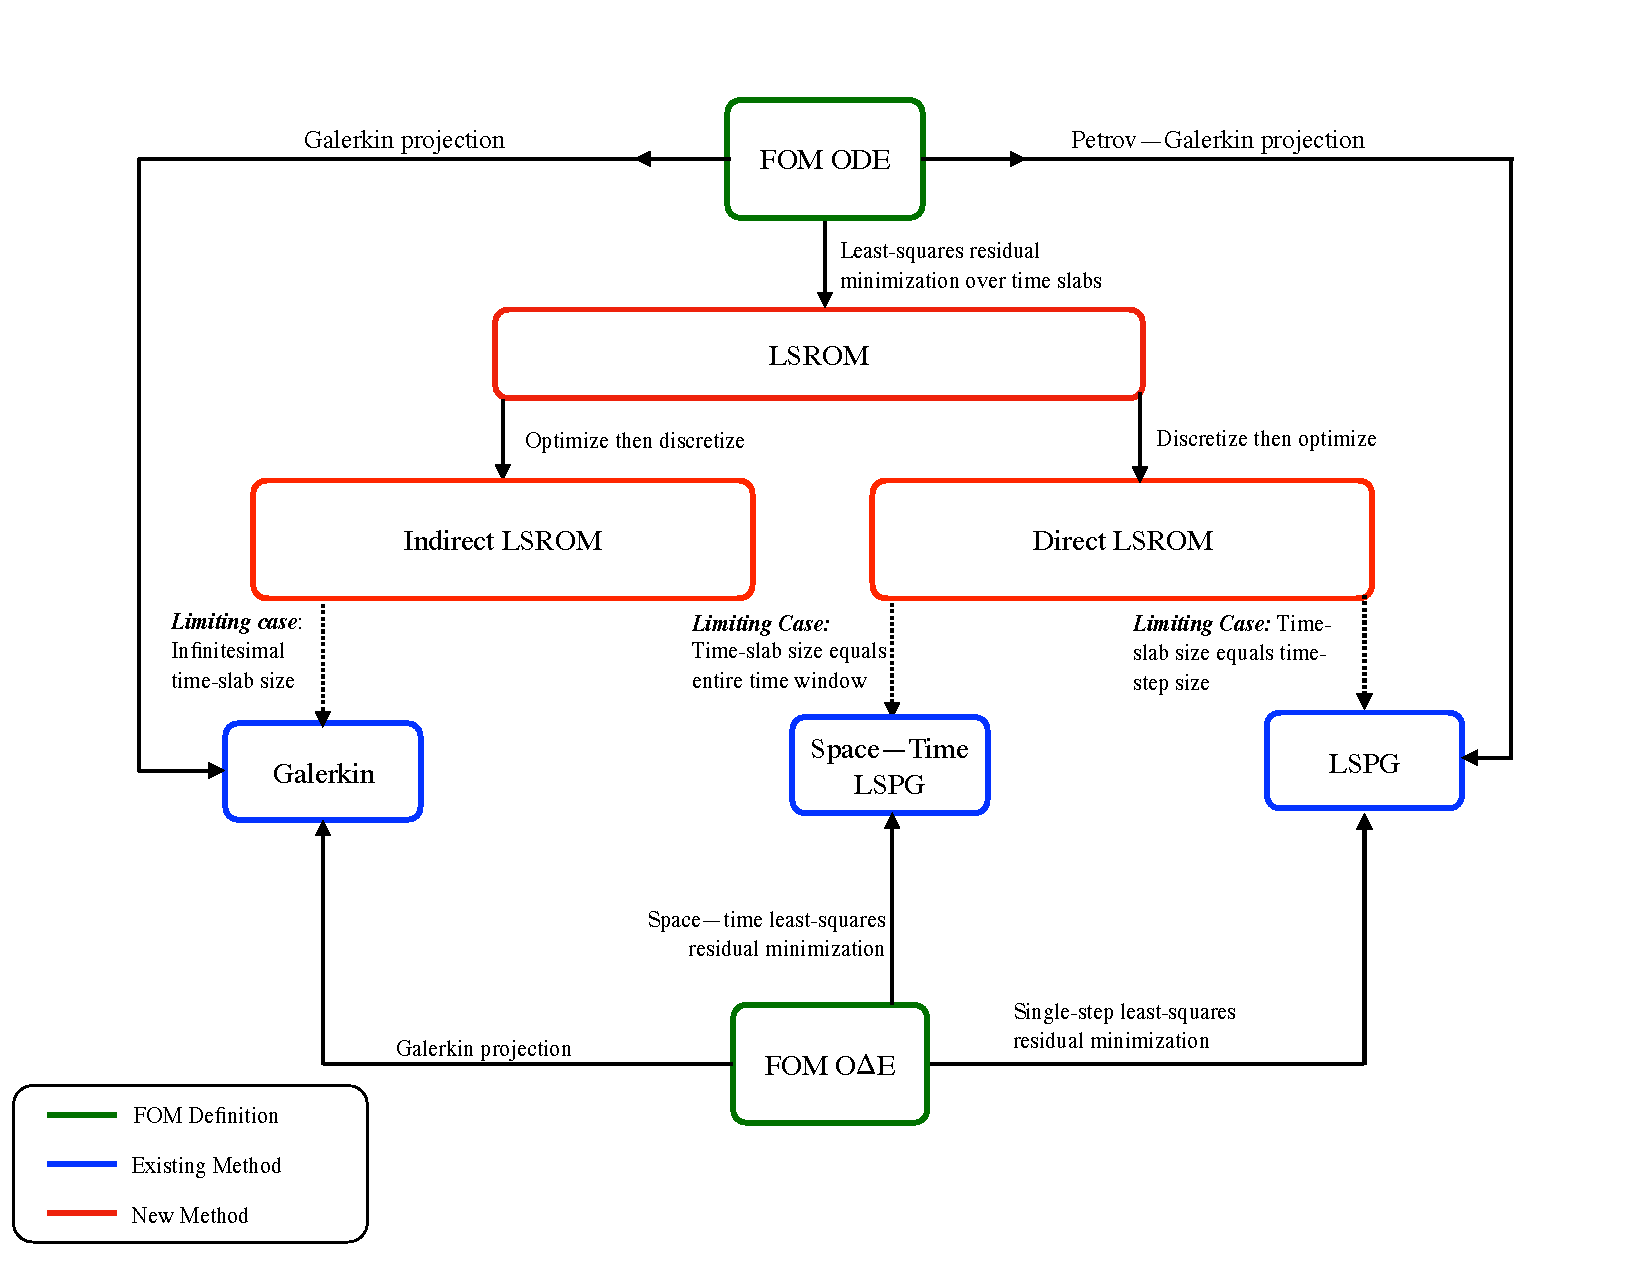
\includegraphics[trim={0.1cm 0cm 1cm 0cm},clip,width=0.99\textwidth]{diagram.pdf} 
\caption{Relationship diagram for the \methodAcronym\ approach for model
	reduction.} 
\label{fig:flowchart} 
\end{centering} 
\end{figure}



 In summary, specific contributions of this work include:
\begin{enumerate}
%\item The development of a time-continuous residual minimization framework for reduced-order models.
\item The \methodNameLower\ (\methodAcronym) approach for dynamical-system
	model reduction. The approach sequentially minimizes the time-continuous
		full-order-model residual over arbitrary time windows.
%\item Support of two space--time trial subspaces: one that reduces the spatial
%	dimension of the FOM only, and one that reduces both the spatial and
%		temporal dimensions of the FOM. 
\item Support of two space--time trial subspaces: one that associates with spatial dimension reduction and 
    one that associates with spatial and temporal dimension reduction.
The former case is of particular
		interest in the \methodAcronym\  contex, as the stationary conditions are
		derived via the Euler--Lagrange equations and comprise a coupled two-point
		Hamiltonian boundary value problem containing a forward and backward
		system. The forward system, which is forced by an auxiliary costate,
		evolves the (spatial) generalized coordinates of the ROM in time. The
		backward system, which is forced by the time-continuous FOM residual
		evaluated about the ROM state, governs the dynamics of the costate. 
	\item Derivation of two solution techniques:
		\textit{discretize then optimize} (i.e., direct) and
		\textit{optimize then discretize} (i.e., indirect). 
	\item Remarks and derivations of conditions under which the
		\methodAcronym\ approach recovers Galerkin, LSPG, and space--time LSPG.
\item Error analysis of the \methodAcronym\ approach using
	trial subspaces associated with spatial dimension reduction.
	This analysis demonstrates that, over a given window, the \methodAcronymROMs\ error 
		is bounded \textit{a priori} by a combination of the
		error at the start of the window and the integrated FOM ODE residual
		evaluated at the FOM state projected onto the trial subspace. 
%As a result,
%		the error bound exhibits exponential growth in the number of time windows
%		(not total time instances), yielding smaller error-bound growth in thime than
%		Galerkin or LSPG projection. \KTC{Check this}
\item Numerical experiments for 
	trial subspaces associated with spatial dimenion reduction, which demonstrate two key findings:
\begin{itemize}
\item Minimizing the residual over a larger time window leads to more stable solutions 
with lower space--time residuals norms.
\item Minimizing the residual over a larger time window does not necessarily
	lead to a more accurate trajectory (as measured in the space--time
		$\elltwo$-norm of the solution). Instead, minimizing the residual over an
		intermediate-sized time window leads to the smallest trajectory error.
\end{itemize}
\end{enumerate}

The paper proceeds as follows: Section~\ref{sec:math}
outlines the mathematical setting for the full-order model, along with Galerkin, LSPG, and
space--time LSPG projection. Section~\ref{sec:tclspg} outlines the proposed \methodAcronym\
\approachKwd. Section~\ref{sec:numerical_techniques}
outlines numerical techniques for solving \methodAcronymROMs, including both direct and
indirect methods. Section~\ref{sec:analysis} provides
equivalence conditions and error analysis for \methodAcronymROMs.
Section~\ref{sec:numerical_experiments} presents numerical experiments.
Section~\ref{sec:conclude} provides conclusions and perspectives.
We denote vector-valued functions with italicized bold symbols (e.g., $\boldsymbol
x$), vectors with standard bold symbols (e.g., $\mathbf{x}$), 
matrices with capital bold symbols (e.g., $\mathbf{X} \equiv \begin{bmatrix}
\mathbf{x}_1 & \cdots & \mathbf{x}_r\end{bmatrix}$), and spaces with
calligraphic symbols (e.g., $\mathcal{X}$). We additionally denote differentiation of a time-dependent 
function with respect to time with the $\dot\ $ operator.
%Model reduction of nonlinear dynamical systems is a growing research area.
%The least-squares Petrov-Galerkin (LSPG) approach has gained popularity as a model reduction technique for nonlinear dynamical systems. Derived at the fully discrete level, the LSPG approach solves a least-squares problem that minimizes the fully discrete residual of the reduced-order model at each time-step. LSPG has been shown to be an effective formulation for nonlinear model reduction on complex problems of interest.
%\begin{comment} 
\section{Mathematical formulation}\label{sec:math}
	We begin by providing the formulation for the full-order model,
	followed by a description of standard model-reduction methods
	classified according to the type of trial subspace they employ.
	\subsection{Full-order model}\label{sec;FOM}
We consider the full-order model to be a dynamical system expressed as a
	system of ordinary differential equations (ODEs)
\begin{equation}\label{eq:FOM}
 \stateFOMDotArg{t}  = \velocity(\stateFOMArg{}{t},t), \qquad \stateFOM(0) =
	\stateFOMIC,\qquad t \in [0,T],
\end{equation}
where  $\stateFOM: [0,T]
	\rightarrow  \RR{\fomdim}$ with $\stateFOM: \timeDummy \mapsto
	\stateFOM(\timeDummy) $ and $\stateFOMDot \equiv {d \stateFOM}/{d\tau}$
	denotes the state implicitly defined as the solution to initial value
	problem~\eqref{eq:FOM}, 
$T \in \RRplus$ denotes the final time, 
 $\stateFOMIC \in \mathbb{R}^{\fomdim}$ denotes the initial condition,
	and $\velocity: \mathbb{R}^{\fomdim} \times [0,T] \rightarrow
	\mathbb{R}^{\fomdim}$ with $(\stateyDiscrete,\timeDummy) \mapsto
	\velocity(\stateyDiscrete,\timeDummy)$ denotes the velocity, which is possibly
	nonlinear in its first argument. For subsequent exposition, we introduce
	$\timeSpace$ to denote the set of (sufficiently smooth) real-valued functions acting on the time
	domain (i.e., $\timeSpace = \{f\,|\,f:[0,T]\rightarrow\RR{}\}$); the
	state can be expressed equivalently as $\stateFOM \in \RR{\fomdim} \otimes
	\timeSpace $.  We refer to the initial value problem defined in
	Eq.~\eqref{eq:FOM} as the ``full-order model" (FOM) ODE. We note that
	although the problem of interest described in the introduction corresponds
	to a parameterized dynamical system, we suppress dependence of the FOM ODE
	\eqref{eq:FOM} on such parameters for notational convenience, as this work
	focuses on devising a model-reduction approach applicable to a specific parameter instance.

Directly solving the FOM ODE~\eqref{eq:FOM} is computationally expensive if
	either the state-space dimension $\fomdim$ is large, or if the time-interval
	length $T$ is large relative to the time step required to numerically
	integrate Eq.~\eqref{eq:FOM}. For time-critical or many-query applications,
	it is essential to replace the FOM ODE~\eqref{eq:FOM} with a strategy that
	enables an approximate trajectory to be computed at lower computational
	cost. Projection-based ROMs constitute one such promising approach. 

\subsection{Reduced-order models}
Projection-based ROMs generate approximate solutions to the FOM
	ODE~\eqref{eq:FOM} by approximating the state in a low-dimensional trial
	subspace. Two types of space--time trial subspaces are commonly used for
	this purpose:\footnote{For both spatial and space--time ROMs of dynamical systems, all trial subspaces are, strictly speaking, space--time subspaces.} 
\begin{enumerate} 
	\item \textit{Subspaces that reduce only the spatial dimension of the full-order
		model (\spatialAcronym)}. These trial subspaces are characterized by a spatial projection operator, associate with a basis that represents the spatial dependence of the state, and are employed in classic model reduction approaches, e.g., Galerkin and LSPG. %These 
%	trial subspaces are commonly used
%		in model-reduction methods based on spatial projection followed by time
%		integration (e.g., the Galerkin and LSPG approaches).
	\item \textit{Subspaces that reduce both the spatial and temporal dimensions of the full-order
		model (\spaceTimeAcronym)}.
These trial subspaces are characterized by a space--time projection operator, associate with a basis that represents the spatial and temporal dependence of the state, and are employed in space--time 
model reduction approaches (e.g., space--time Galerkin~\cite{benner_st}, space--time LSPG~\cite{choi_stlspg}). 
% These trial subspaces are commonly employed in
%		model-reduction methods based on space--time projection (e.g., space--time
%		LSPG).
\end{enumerate}
 We now describe these two types of space--time trial subspaces and their
	application to the Galerkin, LSPG, and space--time LSPG approaches. 

\subsection{\spatialAcronym\ trial subspaces}
At a given time instance 
$t\in[0,T]$,
\spatialAcronym\ trial subspaces approximate the FOM ODE solution
	as $\approxstate(t)\approx\stateFOM(t)$, which is enforced to reside in an
	affine spatial trial subspace of dimension $K\ll\fomdim$ such that
	$\approxstate(t)\in
	\stateIntercept+\trialspace
\subseteq\RR{\fomdim}$, where $\dim(\trialspace) = K$
and $\stateIntercept \in \mathbb{R}^{\fomdim}$ denotes the reference state, which
	is often taken to be the initial condition (i.e., $\stateIntercept = \stateFOMIC$).
Here, the trial subspace
$\trialspace$ 
is spanned by an orthogonal basis such that
$ \trialspace= \Range{\basismat}$
with 
$ \basismat \equiv \begin{bmatrix}  \basisvec_1  & \cdots &  \basisvec_K \end{bmatrix}
	\in \RRStar{\romdim}{\fomdim}$, where $\RRStar{\romdim}{\fomdim}$ denotes the compact Stiefel manifold (i.e.,  $
	\RRStar{\romdim}{\fomdim}\defeq
	\{ \mathbf{X} \in \RR{\fomdim
	\times \romdim}\, \big|\, \mathbf{X}^T \mathbf{X} = \mathbf{I} \}$).
The basis vectors $\basisvec_i$, $i=1,\ldots,K$ are typically constructed
using state snapshots, e.g., via
proper orthogonal decomposition (POD)~\cite{berkooz_turbulence_pod}, the reduced-basis method~\cite{rb_1,rb_2,rb_3,NgocCuong2005,Rozza2008}. 
Thus, at any time instance $t\in[0,T]$, ROMs that employ the  \spatialAcronym\
trial subspace approximate the FOM ODE solution as
\begin{equation}\label{eq:affine_trialspace}
\stateFOMArg{}{t} \approx \approxstate(t) = \basisspace \genstateArg{}{t} + \stateIntercept,
\end{equation}
where $\genstate \in \RR{\romdim} \otimes \timeSpace$ with
$\genstate:\timeDummy\mapsto\genstate(\timeDummy)$
denotes the generalized
coordinates. From the space--time perspective, this is equivalent to approximating the
	FOM ODE solution trajectory $\stateFOM\in\RR{N}\otimes\timeSpace$ with 
	$\approxstate\in \stspaceS$, where
\begin{equation}\label{eq:spatial_subspace}
\begin{split}
& \stspaceS \defeq \trialspace \otimes \timeSpace +
	\stateIntercept\otimes\onesFunction\subseteq\RR{N}\otimes\timeSpace
\end{split}
\end{equation}
with $\onesFunction\in\timeSpace$ defined as
$\onesFunction:\timeDummy\mapsto 1$.
	 
Substituting the approximation~\eqref{eq:affine_trialspace} into the FOM ODE~\eqref{eq:FOM} and performing orthogonal
$\elltwo$-projection of the initial condition onto the trial subspace yields
the overdetermined system of ODEs
\begin{equation}\label{eq:g_truncation}
\basisspace \genstateDotArg{}{t} = \velocity(\basisspace
\genstateArg{}{t} + \stateIntercept,t ), \qquad \genstate(0) = \genstateIC,
	\qquad t \in [0,T],
\end{equation}
where $\genstateDot\equiv {d \genstate}/{d\tau}$.
Because Eq.~\eqref{eq:g_truncation} is overdetermined, a solution may not
exist. Typically, either \textit{Galerkin} or \textit{least-squares
Petrov--Galerkin} projection is employed to reduce the number of equations
such that a unique solution exists. We now describe these two methods.

\subsubsection{Galerkin projection}
The Galerkin approach reduces the number of equations in
Eq.~\eqref{eq:g_truncation} by enforcing orthogonality of the 
residual to the spatial trial subspace in the (semi-)inner product induced by the 
positive (semi-)definite $\fomdim\times\fomdim$ matrix $\stweightingMatArg{}\equiv \stweightingMatOneTArg{ }
\stweightingMatOneArg{ }$ (commonly set to
$\stweightingMatArg{}=\mathbf{I}$), i.e.,
\begin{equation}\label{eq:g_truncation2}
\genstateGalerkinDotArg{}{t} = \massArgnt{n}^{-1} \basisspace^T \stweightingMatArg{} \velocity(\basisspace
\genstateGalerkinArg{}{t} + \stateIntercept,t), \qquad \genstateGalerkin(0) = \genstateIC, \qquad t \in [0,T],
\end{equation}
where $\massArgnt{ } \equiv \basisspace^T \stweightingMatArg{ } \basisspace$
denotes the $K\times K$ positive definite mass matrix.
As demonstrated in Ref.~\cite{carlberg_lspg_v_galerkin}, the Galerkin approach
can be viewed alternatively as a residual-minimization
method, as the Galerkin ODE~\eqref{eq:g_truncation2} is equivalent
to
\begin{equation}\label{eq:GalOptimal}
\genstateGalerkinDotArg{}{t} = \underset{ \genstateyDiscrete \in \RR{\romdim}
	}{\text{arg\,min}} \| \basisspace \hat{\stateyDiscrete} -
	\velocity(\basisspace \genstateGalerkinArg{}{t} + \stateIntercept,t)
	\|_{\stweightingMatArg{}}^2, \qquad \genstate(0) = \genstateIC,
	\qquad t \in [0,T],
%\hat{\mathbf{v}}, %\qquad \genstateGalerkin(0) = \basisspace^T(\stateFOMIC -\stateIntercept), \qquad t \in [0,T].
\end{equation}
where $\|\mathbf{x}\|_{\stweightingMatArg{}}\equiv
\sqrt{\mathbf{x}^T\stweightingMatArg{}\mathbf{x}}$.
Thus, the computed velocity $\genstateGalerkinDotArg{}{t}$ minimizes the
FOM ODE residual evaluated at the state $\basisspace
\genstateGalerkin(t) + \stateIntercept$ and time instance $t$ over the spatial trial
subspace $\trialspace$.
%To perform dimension reduction, 
%To perform dimension reduction, the governing equations are projected by a ``test" basis,
%\begin{equation}\label{eq:g_truncation}
%\testbasis^T \basisspace \frac{d \genstate}{dt} = \testbasis^T \velocity(\basisspace \genstate + \state_0,t; \param ), \qquad t \in [0,T],
%\end{equation}
%The most common choice is to set the test space and trial space to be equivalent, which results in the Galerkin reduced-order model,
%\begin{equation}\label{eq:g_truncation}
%\frac{d \genstate}{dt} = \basisspace^T \velocity(\basisspace \genstate + \state_0,t; \param ), \qquad t \in [0,T],
%\end{equation}
\subsubsection{Least-squares Petrov--Galerkin projection}
Despite its time-instantaneous residual-minimization optimality property 
\eqref{eq:GalOptimal}, the Galerkin approach can yield inaccurate solutions,
particularly if the velocity is not self-adjoint or
is nonlinear. 
Least-squares Petrov--Galerkin (LSPG)
~\cite{carlberg_lspg_v_galerkin,carlberg_thesis,carlberg_gnat,bui_unsteady,bui_thesis}
was developed
as an alternative method that exhibits several advantages over the Galerkin approach.
Rather than minimize the (time-continuous) FOM ODE residual at a time instance (as in Galerkin), LSPG minimizes
the (time-discrete) FOM O$\Delta$E residual 
(i.e., the residual arising after applying time discretization to the FOM ODE)
over a time step.
We now describe the LSPG approach in the case of linear multistep methods;
Ref.~\cite{carlberg_lspg_v_galerkin} also presents LSPG for Runge--Kutta
schemes. 

Without loss of generality, we introduce a uniform time
grid characterized by time step $\Delta t$ and time instances
$t^n = n\Delta
t$, $n=0,\ldots,N_t$.
Applying a linear multistep method to discretize the FOM ODE \eqref{eq:FOM}
with this time grid
yields the FOM O$\Delta$E, which computes the sequence of discrete
solutions
$\stateFOMDiscreteArg{n}( \approx \stateFOM(t^n))$, $n=1,\ldots,N_t$
as the implicit solution to the system of algebraic equations
\begin{equation}\label{eq:lms}
\residLMSArg{n}
	(\stateFOMDiscreteArg{n};\stateFOMDiscreteArg{n-1},\ldots,\stateFOMDiscreteArg{n-k^n})
	= \bz,\qquad n=1,\ldots,N_t,
\end{equation}
where  $k^n$ denotes the number of steps employed by the scheme at the $n$th
time instance and 
$\residLMSArg{n}$ denotes the FOM O$\Delta$E residual defined as
\begin{align*}
\residLMSArg{n} &: (\stateyDiscreteArgnt{n};\stateyDiscreteArgnt{n-1},\ldots,\stateyDiscreteArgnt{n-k^n}) \mapsto  \frac{1}{\Delta t} \sum_{j=0}^{k^n} \alpha^n_j \stateyDiscreteArgnt{n-j} -  \sum_{j=0}^{k^n} \beta^n_j \velocity(\stateyDiscreteArgnt{n-j},t^{n-j}),
\\
&: \RR{\fomdim} \otimes \RR{k^n + 1} \rightarrow \RR{\fomdim}.
\end{align*} 
Here, $\alpha^n_j,\beta^n_j\in\RR{}$, $j=0,\ldots,k^n$ are coefficients
that define the linear multistep method at the $n$th time instance.
%\begin{equation}\label{eq:coarse_implicit_euler_0}
%\residLMS \frac{\stateFOMDiscreteArg{n} - \stateFOMDiscreteArg{n-1}  }{\Delta t} - \velocity(\stateFOMDiscreteArg{n}) = \mathbf{0}, \qquad n = 1,2,\ldots,N_t,
%\end{equation}
%the algebraic FOM O$\Delta$E obtained after an implicit Euler temporal discretization is given by,
%\begin{equation}\label{eq:coarse_implicit_euler_0}
%\frac{\stateFOMDiscreteArg{n} - \stateFOMDiscreteArg{n-1}  }{\Delta t} - \velocity(\stateFOMDiscreteArg{n}) = \mathbf{0}, \qquad n = 1,2,\ldots,N_t,
%\end{equation}
%where $\stateFOMDiscreteArg{n} \approx \stateFOM(t^n)$ denotes the discrete approximation to the state at the $n${th} time instance.

At each time instance on the time grid, LSPG substitutes the \spatialAcronym\ trial subspace approximation
\eqref{eq:affine_trialspace} into the FOM O$\Delta$E~\eqref{eq:lms} and
minimizes the residual, i.e., LSPG sequentially computes the solutions
$\approxstateLSPG^n \approx \stateFOMDiscreteArg{n}$, $n=1,\ldots,
\ntimeSteps$ that satisfy
\begin{equation*}
\approxstateLSPG^n = \underset{\stateyDiscrete \in \trialspace + \stateIntercept }{\text{arg\,min}}|| \lspgWeightingArg{\stateyDiscrete}\residLMSArg{n} (\stateyDiscrete; \approxstateLSPG^{n-1},\ldots,\approxstateLSPG^{n-k^n}) ||_2^2, \qquad n = 1,\ldots,\ntimeSteps,
\end{equation*}
where 
$\lspgWeightingArg{\cdot} \in \RR{\nsamples \times \fomdim}$, with $\romdim
\le \nsamples \le \fomdim$, is a weighting matrix that can be used, e.g., to
enable hyper-reduction by requiring it to have a small number of nonzero
columns. 

As described in the introduction, although numerical experiments have
demonstrated that LSPG often yields more accurate and stable
solutions than Galerkin~\cite{bui_thesis,carlberg_lspg_v_galerkin,carlberg_gnat,carlberg_thesis,parish_apg},
LSPG still suffers from several shortcomings. In particular, LSPG suffers from its complex
dependence on the time discretization, exponentially growing error bounds, and
lack of optimality for the trajectory defined over the entire time domain.

\subsection{\spaceTimeAcronym\ trial spaces and space--time ROMs}

Space--time projection methods that employ \spaceTimeAcronym\ trial
spaces~\cite{choi_stlspg,constantine_strom,URBAN2012203,Yano2014ASC,benner_st,bui_thesis}
aim to overcome the latter two shortcomings of LSPG. Because these methods employ \spaceTimeAcronym\ trial
spaces, they reduce both the spatial and temporal dimensions of the full-order
model; further, they yield error bounds that grow more slowly in time and
their trajectories exhibit an optimality property over the entire time domain. 

\spaceTimeAcronym\ trial subspaces approximate the FOM ODE solution
trajectory
	$\stateFOM\in\RR{N}\otimes \timeSpace$ with an approximation that resides in an
	affine space--time trial subspace of dimension $\stdim\ll\fomdim$, i.e., 
	$\approxstate\in \stspaceST$ with $\dim(\stspaceST) =\stdim $, where
\begin{equation}\label{eq:sttrialspace_def}
 \stspaceST \defeq 
	\Range{\stbasis} + 
	\stateFOMIC\otimes\onesFunction
	\subseteq \RR{N} \otimes \timeSpace.
\end{equation}
%and $\stbasis\in\RR{N \times \stdim}\otimes \timeSpace$ with 
Here $\stbasis \in \RR{\fomdim \times \stdim} \otimes \timeSpace$, with $\stbasis:\timeDummy\mapsto\stbasis(\timeDummy)$ and $\stbasis(0) =
\boldsymbol 0$
denotes the space--time trial basis. 
Thus, at any time instance $t\in[0,T]$, ROMs that employ the
\spaceTimeAcronym\ trial subspace approximate the FOM ODE solution as
\begin{equation}\label{eq:stapprox1}
 \stateFOMArg{}{t} \approx \approxstateArg{}{t}  = \stbasisArg{}{t} \stgenstate + \stateFOMIC,
\end{equation}
where $\stgenstateArg{} \in \RR{\stdim}$ denotes the space--time generalized coordinates. 
Critically, comparing the approximations arising from \spatialAcronym\ and
\spaceTimeAcronym\ trial subspaces in Eqs.~\eqref{eq:affine_trialspace} and \eqref{eq:stapprox1}, respectively,
highlights that the former approximation associates with time-dependent
generalized coordinates, while the latter approximation associates with a
time-dependent basis matrix.

Substituting the approximation~\eqref{eq:stapprox1} into the FOM
ODE~\eqref{eq:FOM} yields
\begin{equation}\label{eq:st_fom}
\stbasisDotArg{}{t} \stgenstate =  \velocity(\stbasisArg{}{t} \stgenstate +
	\stateFOMIC,t) , \qquad t \in [0,T],
\end{equation}
where 
$\stbasisDot\equiv d\stbasis/d\timeDummy$. We note that the initial conditions
are automatically satisfied from the definition of the \spaceTimeAcronym\
trial subspace.

Space--time methods reduce the number of equations in
\eqref{eq:st_fom} to ensure a unique solution exists.
We now outline one such method: space--time least-squares Petrov--Galerkin (ST-LSPG)
~\cite{choi_stlspg}. 
While the space--time Galerkin method~\cite{benner_st} is another alternative, it does not
associate with any residual-minimization principle, and thus we do not discuss
it further.
\subsubsection{Space--time LSPG projection} 
Analogously to LSPG, space--time LSPG~\cite{choi_stlspg}
minimizes the (time-discrete) FOM O$\Delta$E residual, but does so
using the \spaceTimeAcronym\ subspace and simultaneously minimizes this
residual over all $N_t$ time instances.
We first introduce the full space--time FOM O$\Delta$E residual for linear
multistep methods as
\begin{align*}
\residST_{} & \vcentcolon (\stateyDiscreteArg{1}, \ldots
	,\stateyDiscreteArg{N_t};\stateFOMIC) \mapsto \begin{bmatrix}
\residLMSArg{1}(\stateyDiscreteArg{1}; \stateFOMIC) 
%\frac{\stateyDiscreteArg{N_t} - \stateyDiscreteArg{N_t-1}  }{\Delta t} -  \velocity(\stateyDiscreteArg{N_t}) \\
\\ 
%\frac{\stateyDiscreteArg{N_t-1} - \stateFOMDiscreteArg{N_t-2}  }{\Delta t} -  \velocity(\stateyDiscreteArg{N_t-1}) \\
\vdots \\
%\frac{\stateyDiscreteArg{1} - \stateFOMIC }{\Delta t} -  \velocity(\stateyDiscreteArg{1}) \\
\residLMSArg{N_t}(\stateyDiscreteArg{N_t};\stateyDiscreteArg{N_t-1},\ldots,\stateyDiscreteArg{N_t - k^{N_t}}) \end{bmatrix} , \\
& \vcentcolon \RR{\fomdim} \otimes \RR{N_t+1} \rightarrow \RR{\fomdim N_t},
\end{align*}
and define the counterpart function acting on space--time generalized
coordinates:
\begin{align*}
\genresidST_{\text{}} & \vcentcolon (\stgenstatey ;\stateFOMIC) \mapsto \begin{bmatrix}
%\frac{\stateyDiscreteArg{N_t} - \stateyDiscreteArg{N_t-1}  }{\Delta t} -  \velocity(\stateyDiscreteArg{N_t}) \\
\residLMSArg{1}\bigg( \stbasisArg{}{t^1}\stgenstatey + \stateIntercept; \stateFOMIC \bigg)
\\ 
\vdots \\
\residLMSArg{N_t}\bigg( \stbasisArg{}{t^{N_t}}\stgenstatey + \stateIntercept; \stbasisArg{}{t^{N_t-1}}\stgenstatey + \stateIntercept ,\ldots,  \stbasisArg{}{t^{N_t-k^{N_t}}}\stgenstatey + \stateIntercept \bigg)  \\ 
\end{bmatrix} , \\
& \vcentcolon \RR{\stdim} \times \RR{N} \rightarrow \RR{\fomdim N_t}. 
\end{align*}
ST-LSPG computes the space--time generalized coordinates that
minimize the space--time FOM O$\Delta$E residual:
\begin{equation}\label{eq:stlspg}
	\stgenstate_\text{ST-LSPG} = \underset{ \stgenstatey\in\RR{\stdim} }{\text{arg\,min}}|| \lspgWeightingSTArg{\stgenstatey}  \genresidST_{\text{}}(\stgenstatey;\stateFOMIC) ||_2^2, 
\end{equation}
where $\lspgWeightingSTArg{\cdot} \in \RR{n_{st} \times N N_t}$, with $\stdim
\le n_{st} \le N N_t$, is a space--time weighting matrix that can be chosen,
e.g., to enable hyper-reduction.

ST-LSPG overcomes two of the primary shortcomings of LSPG. In particular, it
leads to error bounds that grow sub-quadratically in time rather than
exponentially in time, and it generates entire trajectories that associate
with an optimality property over the entire time domain \cite{choi_stlspg}.
However, it is subject to several challenges. First, the computational cost of
solving Eq.~\eqref{eq:stlspg} scales cubically with the number of space--time
degrees of freedom $\stdim$. This cost is due to the fact that ST-LSPG yields 
dense systems that do not expose any natural mechanism for exploiting
the sequential nature of time evolution. Second, it is unclear how these
methods can be employed for future state prediction, as the space--time trial
basis $\stbasis$ must be defined over the entire time interval of interest
$[0,T]$. Third, ST-LSPG is still strongly tied to the time discretization
employed for the full-order model, as it minimizes the (time-discrete) FOM
O$\Delta$E residual over all time instances.
  
\subsection{Outstanding challenges}
This work seeks to overcome the limitations of existing residual-minimizing
model-reduction methods, and to provide a unifying framework from which
existing methods can be assessed. Specifically, we look to overcome the
complex dependence of LSPG on the time discretization,
exponential time growth of the error bounds for Galerkin and LSPG,
the cubic dependence of the computational cost of ST-LSPG on the number of
degrees of freedom, and the lack of ability for ST-LSPG to perform prediction
in time. We now describe the proposed \methodNameLower\ \approachKwd\ for this
purpose. 
%\end{comment}
%\input{formulation_3}

%\subsection{\spaceTimeAcronym\ trial spaces}\label{sec:wls_spacetime}
%\KTC{Error in first equation. This is the approximate solution not the real
%one. Use parallel language to hwo this was done in the last section for
%S-reduction trial subspaces. Also make sure the basis is zero at the beginning
%of the interval and the affine transformation is taken to be the solution at
%the end of the last window. This will not be too trivial, as the solution on
%the previous slab enters the trial subspace definition.}

%We now briefly consider \spaceTimeAcronym\ trial subspaces. 
The \spaceTimeAcronym\ trial subspace over the $n$th time window approximates
the FOM ODE solution trajectory $\stateFOM\in\RR{N}\otimes\timeSpace$
with $\approxstateArgnt{n} \in \stspaceSTArg{n}$, where
\begin{equation}\label{eq:st_sttrialspace}
 \stspaceSTArg{n} \defeq
 \Range{\stbasisArgnt{n}} + \stateInterceptSTArg{n}\otimes \onesFunctionArg{n} \subseteq \RR{\fomdim} \otimes \timeSpaceArg{n}.
\end{equation}
\EP{Is it wrong to say $\stbasisArg{n}{\cdot} \in \RR{\fomdim \times \stdimArg{n}}$ with $\stbasisArgnt{n}: \timeDummy \mapsto \stbasisArgnt{n}(\timeDummy) \ldots$? I don't particularly like
$\stbasisArgnt{n} \in \RR{\fomdim \times \stdimArg{n}}\otimes\timeSpaceArg{n}$; as the reader I think that $\stbasisArgnt{n}$ can take on all temporal functions.}
Here $\stbasisArgnt{n} \in \RR{\fomdim \times
\stdimArg{n}}\otimes\timeSpaceArg{n}$, $n=1,\ldots,\nslabs$, with $\stbasisArgnt{n}: \timeDummy \mapsto \stbasisArgnt{n}(\timeDummy)$ and $\stbasisArg{n}{\timeStartArg{n}} = \bz$ is the space--time trial basis matrix {function} and $\stateInterceptSTArg{n} \in \RR{\fomdim}$, $n=1,\ldots,\nslabs$ provides the affine transformation. 
To enforce the initial condition and ensure solution continuity across time windows, we set $\stateInterceptSTArg{1} = \stateFOMIC$ and
$\stateInterceptSTArg{n} = \approxstateArg{n-1}{\timeEndArg{n-1}}$ for
$n=2,\ldots,\nslabs$.
At any time instance $t \in [\timeStartArg{n},\timeEndArg{n}]$, the \spaceTimeAcronym\ trial subspace approximates the FOM ODE solution as
 \begin{equation}\label{eq:stapprox}
 \stateFOMArg{n}{t} \approx \approxstateArg{n}{t}  = \stbasisArg{n}{t} \stgenstateArg{n} + \stateInterceptSTArg{n},
\end{equation}
where $\stgenstateArg{n} \in \RR{\stdimArg{n}}$ are the space--time generalized coordinates over the $n$th window. 
\begin{comment}
each window, we introduce the space--time trial subspace
$$ \stateArgnt{n} \in \stspaceSTArg{n} \subseteq \RR{N} \otimes \timeSpaceArg{n},$$
along with the space--time trial basis matrix \textit{function}, 
\begin{align*}
\stbasisArgnt{n} &: t \mapsto \stbasis(t) \\
 &: [\timeStartArg{n},\timeEndArg{n}] \rightarrow  \RR{N \times \stdimArg{n}}  ,%\spaceTrialSpace , \\
\end{align*}
\KTC{shouldn't be $\equiv$. Look earlier for this. the right hand side should
be on the left with $\defeq$.} with $\Range{\stbasisArgnt{n}} + \stateInterceptSTArg{} \equiv \stspaceSTArg{n} $ and where $\stdimArg{n}$ is the number of space--time generalized coordinates over the $n$th window. 
For simplicity we assume the reference state to be equivalent for each time window, although no such requirement is necessary. 
\KTC{Remove all commas before equations unless it makes sense gramatically.
Add the $n$ superscript to $x_{ref}$}
The state over each window is approximated by,
\begin{equation}\label{eq:stapprox}
 \stateFOMArg{n}{t} \approx \approxstateArg{n}{t}  = \stbasisArg{n}{t} \stgenstateArg{n} + \stateInterceptSTArg{},
\end{equation}
%and the state is then approximated by,
%\begin{equation}\label{eq:stapprox}
% \stateArg{n}{t} \approx \approxstateArg{n}{t}  = \stbasisArg{n}{t} \stgenstate + \stateInterceptArg{n},
%\end{equation}
%where $\stgenstateArg{n} \in \RR{\stdimArg{n}}$ are the space--time generalized coordinates over the $n$th window.

\end{comment}
Setting $\stspace^n \leftarrow \stspaceSTArg{n}$ in the
\methodAcronym\ minimization problem~\eqref{eq:tclsrm} implies that
\methodAcronym\ with \spaceTimeAcronym\ trial subspaces sequentially computes
solutions $\stgenstateArg{n}$, $n = 1,\ldots,\nslabs$ that satisfy
\begin{align}\label{eq:obj_gen_slab_spacetime}
\begin{split}
&\underset{\stgenstateyArg{} \in \RR{\stdimArg{n}}}{\text{minimize}}\; \mathcal{J}^n( \stbasisArgnt{n} \stgenstateyArg{} + \stateInterceptSTArg{n} \otimes \onesFunctionArg{n} ).% \\ 
%      &\text{subject to }\;  \stbasisArg{n}{\timeStartArg{n}}\stgenstateyArg{n}  =0
%  \begin{cases} 
%\mathbb{P}^n(\stbasisArgnt{n-1}(\timeEndArg{n-1})\stgenstateArg{n-1})  & n = 2,\ldots,\nslabs, \\ 
%\mathbb{P}^n(\stateFOMIC)
% & n=1. \end{cases}
%%\begin{cases} \genstateyArg{n-1}{\timeEndArg{n-1}} & n = 2,\ldots,\nslabs \\
%\genstateIC & n=1, \end{cases} 
\end{split}
\end{align}
%\begin{align}\label{eq:obj_gen_slab_spacetime}
%\begin{split}
%&\stgenstateArg{n} = \underset{\stgenstatey \in \RR{\stdim}}{\text{arg\,min}}\; \mathcal{J}^n( \stbasisArgnt{n} \stgenstatey + \stateInterceptArg{n} ), \\ 
%      &\text{subject to }\;  \stbasisArg{n}{\timeStartArg{n}}\stgenstateArg{n}  =
%  \begin{cases} 
%\mathbb{P}^n(\stbasisArgnt{n-1}\stgenstateArg{n-1})(\timeEndArg{n-1})  & n = 2,\ldots,\nslabs, \\ 
%\mathbb{P}^n(\stateFOMArgnt{1})(0)
% & n=1. \end{cases}
%%\begin{cases} \genstateyArg{n-1}{\timeEndArg{n-1}} & n = 2,\ldots,\nslabs \\
%%\genstateIC & n=1, \end{cases} 
%\end{split}
%\end{align}

%Inserting the approximation~\eqref{eq:stapprox} into the optimization problem~\eqref{eq:tclsrm}, the
%constrained minimization problem over the $n$th time slab can be re-written as,
%\begin{equation}\label{eq:obj_gen_slab_spacetime} \stgenstate^n =
%\underset{\stgenstatey}{\text{argmin }} \mathcal{J}^n \bigg( \stbasisArgnt{n} \stgenstatey + \stateInterceptArg{n}  \bigg) , \end{equation}
%%\begin{equation}\label{eq:obj_gen_slab} \genstate^n(t) =
%%\underset{\genstatey}{\text{argmin }} \mathcal{J}^n
%%\bigg(\decoder\big(\genstatey(\tau)\big) \bigg) , \end{equation}
%subject to the boundary conditions 
%\begin{equation}\label{eq:bcs_spacetime}
%\stbasisArg{n}{\timeStartArg{n}}\stgenstateArg{n} = \begin{cases} 
%\mathbb{P}^n\stbasisArg{n-1}{\timeEndArg{n-1}}\stgenstateArg{n-1}  & n = 2,\ldots,\nslabs, \\ 
%\mathbb{P}^n \stateFOMIC
% & n=1. \end{cases} \end{equation}
\subsubsection{Stationary conditions} 
The key difference between \spaceTimeAcronym\ and \spatialAcronym\ trial
	subspaces is as follows: generalized coordinates for \spaceTimeAcronym\ trial subspaces 
	comprise a vector in $\RR{\stdimArg{n}}$, while generalized coordinates for
	the \spatialAcronym\ trial subspaces comprise a
	time-dependent vector in
	$\RR{\romdimArg{n}} \otimes \timeSpaceArg{n}$. 
Thus, in the \spaceTimeAcronym\ case, the optimization problem is no longer
	minimizing a functional with respect to a (time-dependent) function, but is minimizing a function with 
respect to a vector.  As such, the first-order optimality conditions can be
	derived using standard calculus. Differentiating the objective function with respect
	to the generalized coordinates and setting the result equal to zero yields 
\begin{equation}\label{eq:st_stationary}
 \intSlabArg{n} \bigg[ \stbasisDotArg{n}{t}^T  - \stbasisArg{n}{t}^T \bigg[\frac{\partial
\velocity}{\partial \stateyDiscrete} (\stbasisDotArg{n}{t} \stgenstateArg{n} +                    
\stateInterceptSTArg{n},t)\bigg]^T  \bigg] \stweightingMatArg{n} \bigg( \stbasisDotArg{n}{t} \stgenstateArg{n}  - \velocity (\stbasisArg{n}{t} \stgenstateArg{n} + \stateInterceptSTArg{n},t) \bigg) dt = \bz.\end{equation}
%subject to the boundary conditions 
%\begin{equation}\label{eq:bcs_spacetime}
%\stbasisArg{n}{\timeStartArg{n}}\stgenstateArg{n} = \begin{cases} 
%\mathbb{P}^n\stbasisArg{n-1}{\timeEndArg{n-1}}\stgenstateArg{n-1}  & n = 2,\ldots,\nslabs, \\ 
%\mathbb{P}^n \stateFOMIC &
%n=1. \end{cases} \end{equation}
Thus, for \spaceTimeAcronym\ trial subspaces, the stationary conditions
	comprise a system of algebraic equations, as opposed to a system of
	differential equations as with \spatialAcronym\ trial subspaces.

%\input{timecont_lspg}
\section{Windowed least-squares framework}\label{sec:tclspg} 
This section
outlines the proposed \methodNameLower\ 
(\methodAcronym) framework. In contrast to (1) the Galerkin approach, 
which minimizes the (time-continuous) FOM ODE residual at a time instance, 
(2) the LSPG approach, 
which minimizes
the (time-discrete) FOM O$\Delta$E residual 
over a time step, and (3) the ST-LSPG approach,  
which minimizes
the  FOM O$\Delta$E residual 
over the entire time interval, the proposed \methodAcronym\ method sequentially minimizes the 
time-continuous FOM ODE residual over a series of arbitrarily defined
\textit{time windows}. The formulation is compatible with both \spatialAcronym\ and \spaceTimeAcronym\ trial subspaces. 
In this section, we start by outlining the \methodAcronym\ formulation  
for a general space--time trial subspace. We then examine the \spatialAcronym\ 
trial subspace, followed by the \spaceTimeAcronym\ trial subspace. In each case, we derive the stationary conditions 
associated with the associated residual-minimization problems.
 %The proposed method can be formulated equivalently from
%two viewpoints. The first formulation corresponds to a sequence of
%minimization problems for the generalized coordinates that minimize the FOM
%ODE residual over each time slab. We refer to this as the 
%\textit{residual-minimization viewpoint}. The second viewpoint corresponds to
%formulating an optimal control problem for the Galerkin ROM. In this
%viewpoint, the \methodAcronym\ method is formulated as an optimal control
%problem in where the objective is to find a ``controller" that minimizes the
%residual of the Galerkin ROM. We refer to this viewpoint as the
%\textit{optimal control viewpoint.}  This section outlines the derivation of the \methodAcronym\ method
%from both the residual minimization and optimal control viewpoints.

%\subsection{Formulation of the Time-Continuous LSPG Method} In contrast to
%the LSPG approach, which minimizes the fully discrete residual over a
%time-step, the present work proposes minimizing the time-continuous FOM ODE
%residual over time slabs. The proposed method can be formulated equivalently
%from two viewpoints. The first approach formulates the problem from a
%standard calculus of variations viewpoint and is analogous to the classic
%residual minimization process used in the LSPG method (but here performed at
%the continuous level). The second viewpoint corresponds to formulating an
%optimal control problem in Lagrange form (which is a specific instance of an
%optimal control problem of Bolza type). In this viewpoint, the
%\methodAcronym\ is formulated as an optimal control problem in where the
%objective is to find a ``controller" that minimizes the residual of the
%Galerkin ROM. We now outline both of these (equivalent) formulations. 
%
\subsection{Windowed least-squares for general space--time trial subspaces} 
We begin by introducing a (potentially nonuniform) partition of the time domain $[0,T]$
into $\nslabs$ non-overlapping windows $[\timeStartArg{n} ,
\timeEndArg{n}]\subseteq[0,T]$ of length $\DeltaSlabArg{n}\defeq\timeEndArg{n} -
\timeStartArg{n}$, $n=1,\ldots,\nslabs$ such that 
$\timeStartArg{1} = 0$, $\timeEndArg{\nslabs} = T$, and
$\timeStartArg{n+1} = \timeEndArg{n}$,
$n=1,\ldots,\nslabs-1$; Fig.~\ref{fig:slab_fig} depicts this partitioning.
\begin{figure} 
\begin{centering} 
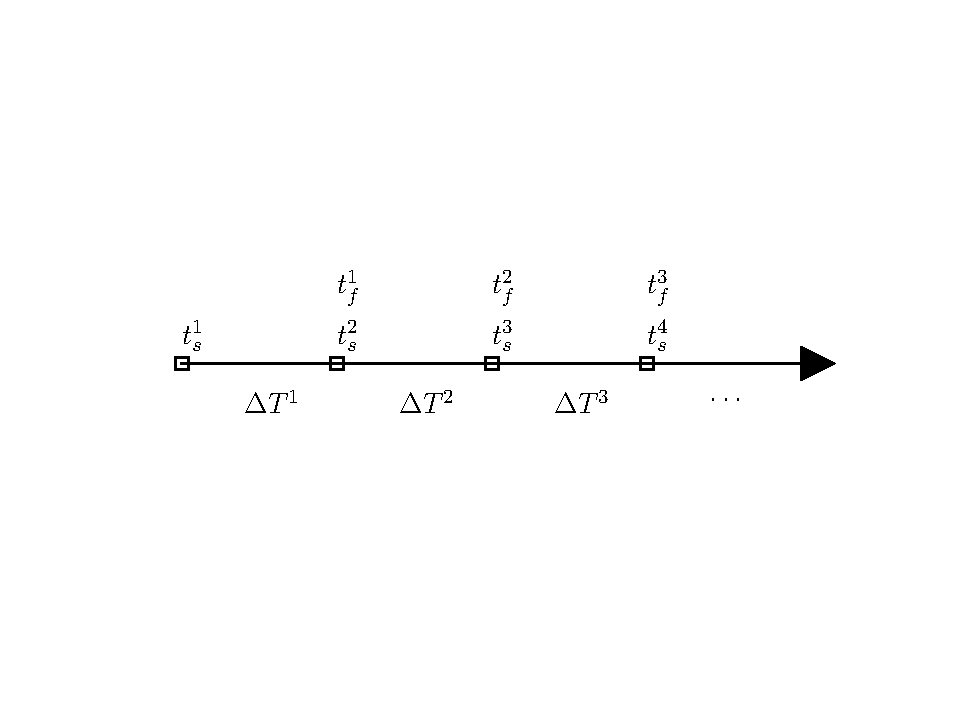
\includegraphics[trim={0.0cm 5cm 0cm 3cm},clip,width=1.0\textwidth]{figs/time_grid.pdf} 
\caption{Partitioning of the time
domain into time windows.} 
\label{fig:slab_fig} 
\end{centering} 
\end{figure}
Over the $n$th time window, we approximate the FOM ODE solution as 
$\approxstate^n(t)\approx \stateFOM(t)$,
$t\in[\timeStartArg{n},\timeEndArg{n}]$, which is enforced to reside in 
the $n$th space--time trial subspace such that
\begin{equation}
\approxstate^n \in \stspace^n \subseteq \RR{N} \otimes \timeSpaceArg{n} , \qquad  n = 1,\ldots,\nslabs,
\end{equation}
where $\stspaceArg{n}$ is the space--time trial subspace over the $n$th window, $\timeSpaceArg{n}$ denotes the set of real-valued functions acting on
$[\timeStartArg{n},\timeEndArg{n}]$ (i.e., $\timeSpaceArg{n} = \{f\,|\,f:[\timeStartArg{n},\timeEndArg{n}]\rightarrow\RR{}\}$)
and
$\approxstate^n \in\RR{\fomdim}\otimes\timeSpaceArg{n}$. For notational purposes, we additionally define the (spatial) trial subspaces at the start of each window as
$$\approxstateArg{n}{\timeStartArg{n}} \in \stspaceBoundStartArg{n} \subset \stspaceArg{n}, \qquad n=1,\ldots,\nslabs. 
%, \qquad 
%\approxstateArg{n}{\timeEndArg{n}} \in \stspaceBoundEndArg{n} \subset \stspaceArg{n}.
$$ 
To outline \methodAcronym, we now define the objective functional over the $n$th window:
\begin{equation}\label{eq:obj}
\begin{split} \mathcal{J}^n &\vcentcolon \statey \mapsto
\frac{1}{2} \int_{\timeStartArg{n}}^{\timeEndArg{n}} \big[ \dot{\statey}(t)
- \velocity(\stateyArg{}{t},t) \big]^T \stweightingMatArgt{n}{t} \big[
\dot{\statey}(t) - \velocity(\stateyArg{}{t},t) \big] d t \\
%&\vcentcolon \RR{\fomdim} \times [\timeStartArg{n},\timeEndArg{n}] \rightarrow
%\RR{}, \end{align}
&\vcentcolon \RR{\fomdim}\otimes \timeSpaceArg{n}  \rightarrow
\RR{}_+, 
\end{split}
\end{equation}
%\begin{align}\label{eq:obj} \mathcal{J}^n &\vcentcolon \state \mapsto
%\frac{1}{2} \int_{\timeStartArg{n}}^{\timeEndArg{n}} \resid(\state)^T
%\stweightingMat \resid(\state) d\tau \\ &\vcentcolon \RR{\fomdim} \times
%[0,T] \rightarrow \RR{}.  \end{align}
where $\stweightingMatArg{n} \equiv \stweightingMatOneTArg{n}
\stweightingMatOneArg{n} \in \RR{\fomdim \times \fomdim}$ denotes a
symmetric positive semi-definite matrix that can enable hyper-reduction, for
example. 
%For notational simplicity, we employ the same weighting matrix for all time windows. 

The \methodAcronym\ framework sequentially computes approximate solutions
$\approxstateArgnt{n}\in\stspace^n$, $n=1,\ldots,\nslabs$, where 
$\approxstateArgnt{n}$ is the solution to the
minimization problem
\begin{equation}\label{eq:tclsrm}
\begin{split}
      &\underset{\statey \in \stspace^n}{\text{minimize}} \; \mathcal{J}^n(\statey), \\
			&\text{subject to } \;  \statey(\timeStartArg{n}) =
\begin{cases}\mathbb{P}^n (\approxstateArgnt{n-1}(\timeEndArg{n-1})) & n = 2,\ldots,\nslabs \\
\mathbb{P}^n( \stateFOMIC)& n=1, \end{cases} 
\end{split}
\end{equation}
%\methodAcronym\ computes a sequence of approximate solutions $\approxstateArgnt{n}$ as the solution to the minimization problem,
%\begin{equation}\label{eq:tclsrm}
%\begin{split}
%       &\approxstateArgnt{n} =  \underset{\statey \in \stspace^n}{\text{arg\,min}} \; \mathcal{J}^n(\statey), \\ 
%      &\text{subject to }\;  \approxstateArg{n}{\timeStartArg{n}} =
%\begin{cases}\mathbb{P}^n (\approxstateArgnt{n-1})(\timeEndArg{n-1}) & n = 2,\ldots,\nslabs \\
%\mathbb{P}^n( \stateFOMArgnt{1})(0)& n=1, \end{cases} 
%\end{split}
%\end{equation}
where $\projectorArg{n} : \RR{\fomdim} \rightarrow \stspaceBoundStartArg{n}$ 
is a (spatial) projector onto the start of the $n$th trial space (e.g., $\elltwo$).

%for \spatialAcronym\ subspaces
%and
%$\mathbb{P}^n (\stateyDiscrete) = \stateyDiscrete$ for \spaceTimeAcronym\ subspaces.
%\methodAcronym\ generates approximations to~\eqref{eq:FOM} by sequentially minimizing
%the FOM ODE residual over the trial space for each time slab.
%\methodAcronym\ is defined as follows,
%\begin{equation}\label{eq:tclsrm}
%\approxstate^n= \underset{\statey \in \stspace^n}{\text{arg\,min } }
%\mathcal{J}^n(\statey), \qquad n = 1,2,...,\nslabs,
%\end{equation}
% subject to
%the boundary condition, \begin{equation*} \approxstate^n(\timeStartArg{n}) =
%\begin{cases}\mathbb{P}^n \approxstate^{n-1}(\timeEndArg{n-1}) & n = 2,\ldots,\nslabs \\
%\mathbb{P}^n \stateFOMIC & n=1, \end{cases} \end{equation*}
%where $\mathbb{P}^n: \RR{N} \rightarrow \stspaceArg{n}$ projects onto the 
%trial space (e.g., an $L^2$ projector).
%and 
%$\approxstate^n :  [\timeStartArg{n} , \timeEndArg{n}] \rightarrow
%\RR{\fomdim}$
%is the approximate solution over the $n$th time slab.% and $\approxstate_0 \in
%\RR{\fomdim}$ is the FOM initial condition
%projected onto the trial space; (e.g., via for $L^2$ projection).
We now define the trial subspaces $\stspaceArg{n}$ considered in this work. In
	particular, we introduce \spatialAcronym\ trial subspaces and
	\spaceTimeAcronym\ trial subspaces tailored for this context. 
We leave further investigation into other approaches, such as nonlinear
	manifolds~\cite{leeCarlberg}, as a subject for future work.
%A variety of trial spaces have been examined in the model-order reduction community.
%The most popular trial space comprises a linear, spatial-projection-only trial space (e.g., Eqns.~\eqref{eq:spatial_subspace}-\eqref{eq:spatial_subspace3}), although recently 
%nonlinear trial spaces~\cite{leeCarlberg} and space--time trial spaces~\cite{choi_stlspg,constantine_strom,2,3} have gained attention. This work focuses on the classic 
%spatial-projection-only trial space, and also briefly considers space--time trial spaces.
%We leave further investigation into other trial spaces as future work.

\subsection{\spatialAcronym\ trial subspaces}
%\KTC{Make sure that $\trialspace$ and $\stateIntercept$ depend on $n$.}
%\KTC{HERE}
The \spatialAcronym\ trial subspace over the $n$th time window approximates
the FOM ODE solution trajectory $\stateFOM\in\RR{N}\otimes\timeSpace$
with $\approxstateArgnt{n} \in \stspaceSArg{n}$, where
\begin{equation}\label{eq:sttrialspace}
 \stspaceSArg{n} \defeq 
	\trialspaceArg{n} \otimes \timeSpaceArg{n} +
	\stateInterceptArg{n}\otimes\onesFunction^n.
\end{equation}
Here, the spatial trial subspaces $\trialspaceArg{n}\subseteq\RR{\fomdim}$,
$n=1,\ldots,\nslabs$ satisfy 
$\trialspaceArg{n}\defeq\Range{\basismatArg{n}}$ with 
$\basismatArg{n}\equiv[\basisvecArg{n}_1\ \cdots\
\basisvecArg{n}_{\romdimArg{n}}]\in
\RRStar{\romdimArg{n}}{\fomdim}
$, the reference state $\stateInterceptArg{n} \in \RR{\fomdim}$, $n=1,\ldots,\nslabs$ provides the affine transformation, 
and  
$\onesFunction^n\in\timeSpaceArg{n}$ is defined as
$\onesFunction^n:\timeDummy\mapsto 1.$
% and  
%$\approxstateArgnt{n}: [\timeStartArg{n},\timeEndArg{n}] \rightarrow  \trialspace$ is the \methodAcronym\ approximation to the state over the $n$th time slab.
Thus, at any time instance $t\in[\timeStartArg{n},\timeEndArg{n}]$, the
\spatialAcronym\ trial subspace in this context 
approximates the FOM ODE solution as
\begin{equation}\label{eq:affine_trialspace_tclsrm}
	\stateFOM(t)\approx \approxstateArgnt{n}(t) = \basismatArg{n}
	\genstateArg{n}{t} + \stateInterceptArg{n},
\end{equation}
where $\genstateArgnt{n} \in \RR{\romdim} \otimes \timeSpaceArg{n}$ with
$\genstateArgnt{n}: \timeDummy\mapsto \genstateArgnt{n}(\timeDummy)
$ denotes the generalized coordinates over the $n$th time window. 

Substituting the approximation~\eqref{eq:affine_trialspace_tclsrm} into the
\methodAcronym\ minimization problem~\eqref{eq:tclsrm} and using $\elltwo$ projection of the 
initial conditions implies that 
\methodAcronym\ with \spatialAcronym\ space--time trial subspaces
sequentially computes solutions
$\genstateArgnt{n}$, $n = 1,\ldots,\nslabs$ that satisfy
%For notational purposes, we define the ``decoder", or ``lifting operator",
%that maps the generalized coordinates to the state-space of the full-order
%model as, \begin{align}\label{eq:decoder} \decoder  \vcentcolon & \;
%\genstatey(t) \mapsto \basisspace \genstatey(t) + \stateIntercept, \\
%\vcentcolon & \; \RR{\romdim}  \rightarrow \RR{\fomdim} .  \end{align}
%With $\state(t) \approx \approxstate(t)  =  \decoder(\genstate(t))$, the
%constrained minimization problem at the $n$th time slab can be re-written as,
%The
%constrained minimization problem over the $n$th time slab can be re-written as,
\begin{equation}\label{eq:obj_gen_slab}
\begin{split}
	& \underset{\genstateyArgnt{} \in \RR{\romdimArg{n}} \otimes \timeSpaceArg{n}
			}{\text{minimize}}\; \mathcal{J}^n(\basismatArg{n} \genstateyArgnt{} +
			\stateInterceptArg{n} \otimes \onesFunction^n), \\ 
      & \text{subject to }\; \genstateyArg{}{\timeStartArg{n}} =
	\begin{cases}
\spatialIC & n = 2,\ldots,\nslabs \\
\genstateICOne & n=1. \end{cases} 
\end{split}
\end{equation}
We emphasize that problem~\eqref{eq:obj_gen_slab} aims to compute the
\textit{function} $\genstate^n$ that minimizes the \textit{functional}
	$\objectiveArg{n}$. 	%corresponds to
%an infinite dimensional minimization problem: the problem 

\subsubsection{Stationary conditions and the Euler--Lagrange equations}
	\KTC{HERE}
	\KTC{Quite a few issues here. Need to make $\mathcal I$ have a superscript
	$n$ everywhere, including (19), (20), need to replace $[0,T]$ with
	$[t_s^n,t_f^n]$ in the function argumentsi, need to make the functions in
	(19) and (20) depend also on the functional $\hat x^n$ (but use a general
	notation for this variable). Need to make sure all the basis $\basismat$
	have arguments throughout as well as the reference states. }

Stationary conditions for optimization problem~\eqref{eq:obj_gen_slab} can be derived via 
	the Euler--Lagrange equations from the
calculus of variations. To outline this process, we begin by defining the
integrand appearing in the objective function $\mathcal{J}^n$ defined in Eq.~\eqref{eq:obj} (in terms of the generalized
coordinates) as 
\begin{equation}\label{eq:integrand}
\begin{split}
 \minintegrandArg{n} & \vcentcolon
(\genstateyDiscreteArgnt{}, \genstateyDiscreteDotArgnt{},\timeDummy) \mapsto \frac{1}{2} \big[
\basisspaceArg{n} \genstateyDiscreteDotArgnt{} - \velocity(\basisspaceArg{n} \genstateyDiscreteArgnt{}
+ \stateInterceptArg{n},\timeDummy ) \big]^T \stweightingMatArgt{n}{t} \big[
\basisspaceArg{n} \genstateyDiscreteDotArgnt{}  - \velocity(\basisspaceArg{n} \genstateyDiscreteArgnt{} +
\stateInterceptArg{n},\timeDummy) \big], \\ & \vcentcolon \RR{\romdimArg{n}} \times \RR{\romdimArg{n}} \times [\timeStartArg{n},\timeEndArg{n}]
 \rightarrow \RRplus .  
\end{split}
\end{equation}
%$$\minintegrand^n(\genstate^n,\dot{\genstate},t)= \frac{1}{2}
%\big[\frac{\partial \decoder}{\partial \genstate} \dot{\genstate} -
%\velocity(\decoder(\genstate)) \big]^T \stweightingMat(t) \big[\frac{\partial
%\decoder}{\partial \genstate} \dot{\genstate} -
%\velocity(\decoder(\genstate)) \big].$$
We also define the quantities
\begin{equation}
\begin{split}
\dIdVArg{n}  & \vcentcolon
(\genstatey , \genstateyDot, \timeDummy) \mapsto \bigg[ \frac{\partial \minintegrandArg{n}}{\partial \genstateyDiscreteDot} (\genstateyArg{}{\timeDummy}, \genstateyDotArg{}{\timeDummy},\timeDummy) \bigg]^T, \\ 
& \vcentcolon  \RR{\romdimArg{n}} \otimes \timeSpaceArg{n} \times \RR{\romdimArg{n}} \otimes \timeSpaceArg{n} \times [\timeStartArg{n},\timeEndArg{n}]
 \rightarrow \RR{\romdimArg{n}} ,
\end{split}
\end{equation}
\begin{equation}
\begin{split}
\dIdYArg{n}  & \vcentcolon
(\genstatey , \genstateyDot, \timeDummy) \mapsto \bigg[ \frac{\partial \minintegrandArg{n}}{\partial \genstateyDiscrete} (\genstateyArg{}{\timeDummy}, \genstateyDotArg{}{\timeDummy},\timeDummy) \bigg]^T, \\ 
& \vcentcolon  \RR{\romdimArg{n}} \otimes \timeSpaceArg{n} \times \RR{\romdimArg{n}} \otimes \timeSpaceArg{n} \times [\timeStartArg{n},\timeEndArg{n}]
 \rightarrow \RR{\romdimArg{n}} ,
\end{split}
\end{equation}
where it is noted we have used Jacobian layout for the scalar-by-vector gradients, i.e., $\dIdVArg{n}$ is a column vector functional.
Using this notation, the Euler--Lagrange equations (see
Appendix~\ref{appendix:eulerlagrange} for the derivation) over the $n$th
time window are given by, 
\begin{equation}\label{eq:el1} 
\begin{split}
& \dIdYArg{n}(\genstateArg{n}{t},\genstateDotArg{n}{t},t) - \dIdVDotArg{n}(\genstateArg{n}{t},\genstateDotArg{n}{t}, t )  = \bz, \\ 
&\genstate^n(\timeStartArg{n})  = \begin{cases} 
\spatialIC &
n=2,\ldots,\nslabs, \\ 
\genstateICOne & n=1,
\end{cases}\\ 
%&\dIdV (\genstateArg{n}{\timeEndArg{n}},\genstateDotArg{n}{\timeEndArg{n}},\timeEndArg{n}) = \bz.
&\dIdVArg{n}(\genstateArg{n}{\timeEndArg{n}},\genstateDotArg{n}{\timeEndArg{n}},\timeEndArg{n})  = \bz.
\end{split} 
\end{equation}
Evaluating the terms in system~\eqref{eq:el1} is an exercise in
vector calculus, and the step-by-step process is given in
Appendix~\ref{appendix:vector_calc}. The resulting system can be written as the 
coupled forward-backward system for $t \in [\timeStartArg{n},\timeEndArg{n} ]$,
%\begin{comment}
%The resulting system of equations is
%given by the second-order differential equation,
%%$$ \bigg[\basisspace^T \bigg[\frac{\partial \velocity}{\partial \state}
%%\bigg]^T \stweightingMat  +  \frac{d}{dt} \bigg] \bigg(  \basisspace^T
%%\stweightingMat \basisspace \dot{\genstate}   -  \basisspace^T
%%\stweightingMat \velocity \bigg) = 0,$$
%\EP{Working on this}
%\begin{equation}\label{eq:clspg_2ord}
%\begin{split} 
%&\bigg[\basisspace^T \bigg[\frac{\partial
%\velocity}{\partial \stateyDiscreteArgnt{}} (\basisspace \genstateArg{n}{t} +
%\stateIntercept,t)\bigg]^T \stweightingMatArgt{n}{t} + \basisspace^T
%\stweightingMatArgt{n}{t} \bigg] \bigg(  \basisspace
%\genstateDDotArg{n}{t}    -  \velocityDot(\basisspace \genstateArg{n}{t} + \stateIntercept,t) \bigg) = \bz, \qquad t \in  [\timeStartArg{n},\timeEndArg{n}],
%\\
%&\bigg[\basisspace^T \bigg[\frac{\partial
%\velocity}{\partial \stateyDiscreteArgnt{}} (\basisspace \genstateArg{n}{t} +
%\stateIntercept,t)\bigg]^T \stweightingMatArgt{n}{t} + \basisspace^T
%\stweightingMatArgt{n}{t} \frac{d}{dt} \bigg] \bigg(  \basisspace
%\genstateDotArgnt{n}    -  \velocity^*(\basisspace \genstateArgnt{n} + \stateIntercept,t) \bigg) = \bz, \qquad t \in  [\timeStartArg{n},\timeEndArg{n}],
%\\
%%& \genstateArg{n}{ \timeStartArg{n}} = \genstateArg{n-1}{\timeEndArg{n-1}},
%%\\
%&\genstate^n( \timeStartArg{n})  = \begin{cases}
%\genstate^{n-1}(\timeEndArg{n-1}) & n=2,\ldots,\nslabs, \\
%\basisspace^T(\stateFOMIC - \stateIntercept) & n=1, \end{cases}\\ 
%& 
%\basisspace^T \stweightingMatArgt{n}{\timeEndArg{n}} \basisspace \genstateDotArg{n}{\timeEndArg{n}}  -
%\basisspace^T \stweightingMatArgt{n}{\timeEndArg{n}}
%\velocity(\basisspace \genstateArg{n}{\timeEndArg{n}} + \stateIntercept,\timeEndArg{n}) = \bz.  
%\end{split}
%\end{equation}
%The second-order system~\eqref{eq:clspg_2ord} can be written equivalently as two first-order
%equations by introducing an auxiliary ``\adjointStr", or ``costate", variable. %To do this, first
%Defining the costate over the $n$th window as, 
%\begin{equation}\label{eq:costate_def}
%\begin{split}
%\adjointArgnt{n} &: t \mapsto \genstateDotArg{n}{t}  -  \mass^{-1} \basisspace^T \stweightingMatArgt{n}{t}\velocity(\veloargsromn) ,\\
%&: [\timeStartArg{n},\timeEndArg{n}] \rightarrow \RR{K} ,
%\end{split}
%\end{equation}
%%\velocity(\veloargsromn)  
%%\adjointArg{n}{t}
%%\defeq 
%%\genstateDotArg{n}{t}  -  \mass^{-1} \basisspace^T \stweightingMatArgt{n}{t}
%%\velocity(\veloargsromn) , \end{align}
%%\basisspace \frac{d \genstate}{dt}  -   \velocity =  \adjoint  , \qquad
%%\genstate(t=0) = \genstate_0 \end{equation}
%where
%$\massArgnt{n} \equiv \basisspace^T \stweightingMatArgt{n}{t} \basisspace$ is the
%mass matrix,
%we can manipulate the system~\eqref{eq:clspg_2ord} (see
%Appendix~\ref{appendix:vector_calc}) to obtain a coupled forward-backward
%system for $t \in  [\timeStartArg{n},\timeEndArg{n}]$,
%\end{comment}
%%%% HERE
\begin{align}\label{eq:lspg_continuous} 
&\massArg{n}   \genstateDotArg{n}{t}  -  [\basisspaceArg{n}]^T
\stweightingMatArgt{n}{t} \velocity(\veloargsromn) =  \massArg{n} \adjointArg{n}{t} , \\
%\end{equation} \begin{equation}\label{eq:lspg_adjoint}
\begin{split}
 &\massArg{n}  \adjointDotArg{n}{t}  + [\basisspaceArg{n}]^T \bigg[\frac{\partial
\velocity}{\partial \stateyDiscrete} (\veloargsromn) \bigg]^T \stweightingMatArgt{n}{t} \basisspaceArg{n}
 \adjointArg{n}{t} = -[\basisspaceArg{n}]^T \big[
\frac{\partial \velocity}{\partial \stateyDiscrete}(\veloargsromn) \big]^T \\& \hspace{1.7 in} \stweightingMatArgt{n}{t} \big( \mathbf{I} -
\basisspaceArg{n} [\massArg{n}]^{-1} [\basisspaceArg{n}]^T \stweightingMatArgt{n}{t} \big)
 \big( \basisspaceArg{n} \genstateDotArg{n}{t} -
\velocity(\veloargsromn) \big), \label{eq:lspg_adjoint}
\end{split}
 \\ &
\genstateArg{n}{\timeStartArg{n}} = \begin{cases}
\spatialIC & n=2,\ldots,\nslabs, \label{eq:lspg_bcs1}\\
\genstateICOne & n=1, \end{cases}\\ &
\adjointArg{n}{\timeEndArg{n}} = \boldsymbol 0, \label{eq:lspg_bcs} 
\end{align}
where 
\begin{equation}\label{eq:costate_def}
\begin{split}
\adjointArgnt{n} &: \timeDummy \mapsto \genstateDotArg{n}{\timeDummy}  -  [\massArg{n}]^{-1} [\basisspaceArg{n}]^T \stweightingMatArgt{n}{\timeDummy}\velocity(\basisspaceArg{n} \genstateArg{n}{\timeDummy} + \stateInterceptArg{n} , \timeDummy ) ,\\
&: [\timeStartArg{n},\timeEndArg{n}] \rightarrow \RR{\romdimArg{n}} ,
\end{split}
\end{equation}
is the adjoint, or ``costate" variable, $\adjointDotArgnt{n} \equiv d \adjointArgnt{n}/ d\tau$, and $\massArg{n} \equiv \basisspaceTArg{n} \stweightingMatArg{n} \basisspaceArg{n}$ is a mass matrix. 
%where
%$\massArgnt{n}= \basisspace^T \stweightingMatArgt{n}{t} \basisspace$ is the
%mass matrix.
%\end{equation}
Equation~\eqref{eq:lspg_continuous} is equivalent to a Galerkin reduced-order
model forced by the costate variable, $\adjointArgnt{n}$.
Equation~\eqref{eq:lspg_adjoint} is typically referred to as the adjoint
equation, and corresponds to a linear equation that is forced by the residual.
It is worth noting that both ODEs~\eqref{eq:lspg_continuous}
and~\eqref{eq:lspg_adjoint} can be hyper-reduced through, e.g.,
collocation, (discrete) empirical interpolation, Gappy POD, etc.~\cite{everson_sirovich_gappy,eim,qdeim_drmac}. The
coupled system defined by the system~\eqref{eq:lspg_continuous}--\eqref{eq:lspg_bcs} can be interpreted as an ``optimally controlled"
ROM. The adjoint equation controls the forward model by enforcing the minimum
residual condition.
%Note that, $$ \basisspace^T \bigg[\frac{\partial \velocity}{\partial \state}
%\bigg]^T \basisspace \adjoint =  \basisspace^T \bigg[\frac{\partial
%\velocity}{\partial \state} \bigg]^T \stweightingMat \basisspace \adjoint .$$

A simplification is obtained in the basic case %with no
%hyper-reduction/weighting 
where $\stweightingMatArg{n} = \mathbf{I}$.
The system becomes
\begin{align*}\label{eq:lspg_continuous_simle} & \genstateDotArg{n}{t}  -
\basisspaceTArg{n}  \velocity(\veloargsromn) =  \adjointArg{n}{t} , \\
%\end{equation} \begin{equation}\label{eq:lspg_adjoint}
 &\adjointDotArg{n}{t}   + \basisspaceTArg{n} \bigg[\frac{\partial
\velocity}{\partial \stateyDiscrete}(\veloargsromn)\bigg]^T \basisspaceArg{n} \adjointArg{n}{t} = \\
&\hspace{2 in} \basisspaceTArg{n} \bigg[
\frac{\partial \velocity}{\partial \stateyDiscrete} (\veloargsromn) \bigg]^T \big( \mathbf{I} -   \basisspaceArg{n} \basisspaceTArg{n}
\big)    \velocity(\veloargsromn) , \\ & \genstateArg{n}{\timeStartArg{n}} =
\begin{cases} \basisspaceTArg{n}(\basisspaceArg{n-1}\genstateArg{n-1}{\timeEndArg{n-1}} - \stateInterceptArg{n})& n=2,\ldots,\nslabs, \\
\genstateICOne& n=1, \end{cases}\\
&\adjointArg{n}{\timeEndArg{n}} = \boldsymbol 0 .  \end{align*}
\begin{remark}
Solutions to the Euler--Lagrange equations correspond to stationary points 
of the objective functional~\eqref{eq:obj_gen_slab}. There are no guarantees, 
however, that a stationary point is a minimum. In general, the stationary 
points could be a maximum, a saddle point, a local minimum, etc.
\end{remark}

\subsubsection{Formulation as an optimal control problem of Lagrange type}\label{sec:optimal_control} 
The Euler--Lagrange equations expose that~\eqref{eq:lspg_continuous}--\eqref{eq:lspg_bcs} can be alternatively formulated as a Lagrange
problem from optimal control. To this end, consider the Galerkin ROM over the $n$th window, 
$$ \basisspaceTArg{n} \stweightingMatArgt{n}{t} \basisspaceArg{n}
 \genstateGalerkinDotArg{n}{t} - \basisspaceTArg{n} \stweightingMatArgt{n}{t}
\velocity(\veloargsromn) = \bz.$$
We introduce now the controller $\controllerArgnt{n} \in \RR{\romdim} \otimes \timeSpaceArg{n}$ 
and state that a residual minimizing controller exists such that \methodAcronym\ can be written as 
\begin{equation}\label{eq:controlled_rom}
 \basisspaceTArg{n}
\stweightingMatArgt{n}{t} \basisspaceArg{n} \genstateDotArg{n}{t}  - \basisspaceTArg{n}
\stweightingMatArgt{n}{t}\velocity(\veloargsromn) = \controllerArg{n}{t}. 
 \end{equation}
%where $\mass \defeq \big[ \basisspace^T \stweightingMat \basisspace]^{-1} \in
%\RR{\romdim \times \romdim}$ is the \textit{mass matrix}. 
We now demonstrate how to find this controller.
Before doing so, it is noted that~\eqref{eq:controlled_rom} displays commonalities with \textit{subgrid-scale}
methods~\cite{iliescu_pod_eddyviscosity,iliescu_vms_pod_ns,iliescu_ciazzo_residual_rom,parish_apg,wentland_apg,Wang:269133,San2018},
in where an additional term is added to the reduced-order model so-as to
account for the truncated dynamics. 

We start by defining a \textit{Lagrangian} that measures the residual norm as a function of the state and controller, 
\begin{equation}\label{eq:obj_controller}
\begin{split}
%\objectiveControlArg{n}(\stateArg{}{t}) = \frac{1}{2}
%\int_{\timeStartArg{n}}^{\timeEndArg{n}} \big[ \basisspace
%\dot{\genstate}(\tau) - \velocity(\stateArg{}{\tau} ) \big]^T
%\stweightingMat(\tau) \big[ \dot{\state}(\tau) - \velocity(\stateArg{}{\tau})
%\big] d \tau, \objectiveControlArg{n}(\genstateArg{}{t},\controllerArg{}{t})
%= \\ \frac{1}{2} \bigg[ \basisspace \bigg(  \mass^{-1}\basisspace^T
%\stweightingMat\velocity(\basisspace \genstate) + \mass^{-1}\controller
%\bigg) - \velocity(\basisspace \genstate ) \bigg]^T \stweightingMat(t) \bigg[
%\basisspace \bigg(  \mass^{-1}\basisspace^T
%\stweightingMat\velocity(\basisspace \genstate) + \mass^{-1}\controller
%\bigg) - \velocity( \basisspace  \genstate ) \bigg] , \\
 \objectiveControlArg{n} &:  (\genstateyDiscreteArgnt{},\controllerDiscreteDumArgnt{},\timeDummy)
\mapsto \frac{1}{2} \bigg[ \basisspaceArg{n} \bigg(  [\massArg{n}]^{-1}\basisspaceTArg{n}
\stweightingMatArgt{n}{t}  \velocity(\basisspaceArg{n} \genstateyDiscreteArgnt{} +
\stateInterceptArg{n},\timeDummy) + [\massArg{n}]^{-1}\controllerDiscreteDumArgnt{} \bigg) -
\velocity(\basisspaceArg{n} \genstateyDiscreteArgnt{} + \stateInterceptArg{n},\timeDummy) \bigg]^T
\stweightingMatArgt{n}{t}  \\ & \hspace{1.5 in}\bigg[ \basisspaceArg{n} \bigg(
[\massArg{n}]^{-1}\basisspaceTArg{n} \stweightingMatArgt{n}{t}\velocity(\basisspaceArg{n}
\genstateyDiscreteArgnt{} + \stateInterceptArg{n},\timeDummy) + [\massArg{n}]^{-1}\controllerDiscreteDumArgnt{}
\bigg) - \velocity( \basisspaceArg{n}  \genstateyDiscreteArgnt{} + \stateInterceptArg{n},\timeDummy ) \bigg]
, \nonumber \\ & : \RR{\romdimArg{n}} \times \RR{\romdimArg{n}} \times [\timeStartArg{n},\timeEndArg{n}] \rightarrow \RR{},
 %\int_{\timeStartArg{n}}^{\timeEndArg{n}}
 %\objectiveControlArg{n}(\genstateArg{}{\tau},\controllerArg{}{\tau}) d\tau =
 %\\ \frac{1}{2} \int_{\timeStartArg{n}}^{\timeEndArg{n}} \bigg[ \basisspace
 %\bigg(  \mass^{-1}\basisspace^T \stweightingMat\velocity(\basisspace
 %\genstate) + \mass^{-1}\controller \bigg) - \velocity(\basisspace \genstate
 %) \bigg]^T \stweightingMat(\tau) \bigg[ \basisspace \bigg(
 %\mass^{-1}\basisspace^T \stweightingMat\velocity(\basisspace \genstate) +
 %\mass^{-1}\controller \bigg) - \velocity( \basisspace  \genstate ) \bigg] d
 %\tau,
\end{split}
\end{equation}
where it is noted that, by Eq.~\eqref{eq:controlled_rom}, $
[\massArg{n}]^{-1}\basisspaceTArg{n} \stweightingMatArg{n} \velocity(\basisspaceArg{n} \genstateArg{n}{t} + \stateInterceptArg{n} ,t) +
[\massArg{n}]^{-1}\controllerArg{n}{t}  = \genstateDotArg{n}{t}.$ 
Hence~\eqref{eq:obj_controller} is a measure of the same residual as in~\eqref{eq:obj}.  The \methodAcronym\ approach with \spatialAcronym\ trial subspaces can be formulated as an ``optimal control" 
method that sequentially computes the controller $\controllerArgnt{n}$, $n=1,\ldots,\nslabs$, that satisfies 
\begin{equation}\label{eq:tclspg_oc1a} 
\begin{split}
&\underset{\controllerDumArgnt{} \in \RR{\romdimArg{n}}\otimes \timeSpaceArg{n} }{\text{minimize } } 
\int_{\timeStartArg{n}}^{\timeEndArg{n}}
\objectiveControlArg{n}(\genstateArg{n}{t},\controllerDumArg{}{t},t)dt, 
 \\
&\text{subject to } \;  \left\{\begin{array}{l} 
 \basisspaceTArg{n} \stweightingMatArgt{n}{t}
\basisspaceArg{n}  \genstateDotArg{n}{t}  - \basisspaceTArg{n}
\stweightingMatArgt{n}{t} \velocity(\veloargsromn) =\controllerDumArg{}{t}, \\
 \genstateArg{n}{\timeStartArg{n}} =
\begin{cases} \spatialIC `& n = 2,\ldots,\nslabs,
 \\ \genstateICOne & n=1. \end{cases} \end{array} \right.
% \genstateArg{n-1}{\timeEndArg{n-1}}.
\end{split}
\end{equation}
%\begin{equation}\label{eq:tclspg_oc1a} 
%\begin{split}
%&\controllerArgnt{n} =
%\underset{\controllerDumArgnt{} }{\text{arg\,min } } 
%\int_{\timeStartArg{n}}^{\timeEndArg{n}}
%\objectiveControlArg{}(\genstateArg{n}{t},\controllerDumArg{}{t},t)dt, 
% \\
%&\text{subject to } \;  \left\{\begin{array}{l} 
% \basisspace^T \stweightingMatArgt{n}{t}
%\basisspace \frac{d}{dt} \genstateArg{n}{t}  - \basisspace^T
%\stweightingMatArgt{n}{t} \velocity(\basisspace \genstateArg{n}{t} +
%\stateIntercept,t) =\controllerArg{n}{t}, \\
% \genstateArg{n}{\timeStartArg{n}} =
%\begin{cases} \genstate^{n-1}(\timeEndArg{n-1} ) & n = 2,\ldots,\nslabs,
% \\ \basisspace^T(\stateFOMIC - \stateIntercept) & n=1. \end{cases} \end{array} \right.
%% \genstateArg{n-1}{\timeEndArg{n-1}}.
%\end{split}
%\end{equation}
%Noting that
%$$\basisspace^T \stweightingMat \basisspace \dot{\genstate} = \basisspace^T \controller + \basisspace^T \stweightingMat \velocity(\basisspace \genstate).$$
%$$\basisspace \dot{\genstate} =  \basisspace \controller + \basisspace \basisspace^T \velocity(\basisspace \genstate).$$
%Then
%\begin{equation}\label{eq:obj}
%\objectiveControlArg{n}(\stateArg{}{t}) = \frac{1}{2} \int_{\timeStartArg{n}}^{\timeEndArg{n}} \big[\basisspace \controller + (\basisspace \basisspace^T  - \mathbf{I} )\velocity(\basisspace \genstate)   ) \big]^T \stweightingMat(\tau) \big[\basisspace \controller + (\basisspace \basisspace^T - \mathbf{I}) \velocity(\stateArg{}{\tau})  \big] d \tau,
%\end{equation}
The solution to the system~\eqref{eq:tclspg_oc1a} is equivalent of that defined by~\eqref{eq:obj_gen_slab}. 
This can be demonstrated via the \textit{Pontryagin Maximum Principle} (PMP)~\cite{optimal_control_book}. To this end, we introduce the Lagrange multiplier (costate) 
$\adjointOCArgnt{n} \in \RR{\romdim} \otimes \timeSpaceArg{n}$ and define the Hamiltonian, 
\begin{equation}\label{eq:hamiltonian}
\begin{split}
\hamiltonianArg{n} \; &: \;  (\genstateyDiscreteArgnt{},\adjointDiscreteDumArgnt{},\controllerDiscreteDumArgnt{},\timeDummy) \mapsto 
 \adjointDiscreteDumArgnt{T} \bigg[  [\massArg{n}]^{-1}\basisspaceTArg{n} \stweightingMatArgt{n}{t}\velocity(\basisspaceArg{n} \genstateyDiscreteArgnt{} + \stateInterceptArg{n},\timeDummy) + [\massArg{n}]^{-1}\controllerDiscreteDumArgnt{} \bigg] +  \objectiveControlArg{n}(\genstateyDiscreteArgnt{},\controllerDiscreteDumArgnt{},\timeDummy) \\
&: \; \RR{\romdimArg{n}} \times \RR{\romdimArg{n}} \times \RR{\romdimArg{n}} \times [\timeStartArg{n},\timeEndArg{n}] \rightarrow \RR{}.
\end{split}
\end{equation} 
The Pontryagin Maximum Principle states that solutions of the optimization problem~\eqref{eq:tclspg_oc1a} must satisfy the 
following conditions over the $n$th window,
\begin{align*}%\label{eq:hamiltonian_sys}
&\genstateDotArg{n}{t} = \frac{\partial \hamiltonianArg{n}}{\partial \adjointDiscreteDumArgnt{}{}}(\genstateArg{n}{t},\adjointOCArg{n}{t},\controllerArg{n}{t},t),\\% \qquad \genstate(t_0(n)) = \genstate^{n-1}(t_1(n-1))\\
&\adjointOCDotArg{n}{t}= - \frac{\partial \hamiltonianArg{n}}{\partial \genstateyDiscreteArgnt{}{}}(\genstateArg{n}{t},\adjointOCArg{n}{t},\controllerArg{n}{t},t),\\% \qquad \adjoint^n(t_1(n)) = 0\\
&\frac{\partial \hamiltonianArg{n}}{\partial \controllerDiscreteDumArgnt{}{}} (\genstateArg{n}{t},\adjointOCArg{n}{t},\controllerArg{n}{t},t) = \boldsymbol 0, \\
& \genstateArg{n}{\timeStartArg{n}} =
\begin{cases} \spatialIC & n = 2,\ldots,\nslabs,
 \\ \genstateICOne& n=1,\end{cases} \\
&\adjointOCArg{n}{\timeEndArg{n}}= \bz.
\end{align*}
Evaluation of the required gradients (Appendix~\ref{appendix:optimal_control}) yields the system to be solved over the $n$th window for $t \in [\timeStartArg{n},\timeEndArg{n}]$,
\begin{equation}\label{eq:sys_oc1}
\begin{split}
&\massArg{n}  \genstateDotArg{n}{t}  -  \basisspaceTArg{n} \stweightingMatArgt{n}{t} \velocity(\veloargsromn) =  \controllerArg{n}{t} , \\
%\end{equation}
%\begin{equation}\label{eq:lspg_adjoint}
 & \adjointOCDotArg{n}{t}  + \basisspaceTArg{n} \bigg[\frac{\partial \velocity}{\partial \stateyDiscrete} (\veloargsromn) \bigg]^T \stweightingMatArgt{n}{t} \basisspaceArg{n} [\massArg{n}]^{-1} \adjointOCArg{n}{t} =  \basisspaceTArg{n} \big[ \frac{\partial \velocity}{\partial \stateyDiscrete}(\veloargsromn) \big]^T \\
& \hspace{1.8in} \stweightingMatArgt{n}{t} \big( \mathbf{I} -   \basisspaceArg{n} [\massArg{n}]^{-1} \basisspaceTArg{n}  \stweightingMatArgt{n}{t} \big)  \big( \basisspaceArg{n}\genstateDotArg{n}{t}  -   \velocity(\veloargsromn) \big) \\%\label{eq:sys_oc2} \\
&\controllerArg{n}{t} = -\adjointOCArg{n}{t} \\%\label{eq:sys_oc3}, \\
& \genstateArg{n}{\timeStartArg{n}} = 
\begin{cases}
\spatialIC& n=2,\ldots,\nslabs, \\
\genstateICOne & n=1,  
\end{cases} \\%\label{eq:sys_oc4} \\
& \adjointOCArg{n}{\timeEndArg{n}} = \boldsymbol 0. \\%\label{eq:sys_oc5}.
\end{split}
\end{equation}
The system~\eqref{eq:sys_oc1} is seen to be equivalent to that defined by the system~\eqref{eq:lspg_continuous}--\eqref{eq:lspg_bcs} (perform 
the change of variables $\controllerArgnt{n} = \massArg{n} \adjointArgnt{n}$ and $\adjointOCArgnt{n} = -\massArg{n} \adjointArgnt{n}$).  
Thus, \methodAcronym\ with \spatialAcronym\ trial subspaces can be formulated as an optimal control problem: \methodAcronym\ finds a controller that modifies the Galerkin ROM such that the residual minimization objective is achieved. In addition to commonalities with optimal control problems, this second formulation displays commonalities with subgrid-scale modeling techniques, in where an additional term is added to the reduced-order model to account for the impact of the truncated modes. \methodAcronym\ can thus be interpreted as a subgrid-scale modeling technique, in where a residual minimizing subgrid-scale model is constructed.

\begin{remark}
The Euler--Lagrange equations comprise a Hamiltonian system. This imbues \methodAcronym\ with \spatialAcronym\ trial subspaces with certain properties; e.g., for autonomous systems the Hamiltonian~\eqref{eq:hamiltonian} is conserved. 
\end{remark} 


\subsection{\spaceTimeAcronym\ trial spaces}\label{sec:wls_spacetime}
%\KTC{Error in first equation. This is the approximate solution not the real
%one. Use parallel language to hwo this was done in the last section for
%S-reduction trial subspaces. Also make sure the basis is zero at the beginning
%of the interval and the affine transformation is taken to be the solution at
%the end of the last window. This will not be too trivial, as the solution on
%the previous slab enters the trial subspace definition.}

%We now briefly consider \spaceTimeAcronym\ trial subspaces. 
The \spaceTimeAcronym\ trial subspace over the $n$th time window approximates
the FOM ODE solution trajectory $\stateFOM\in\RR{N}\otimes\timeSpace$
with $\approxstateArgnt{n} \in \stspaceSTArg{n}$, where
\begin{equation}\label{eq:st_sttrialspace}
 \stspaceSTArg{n} \defeq
 \Range{\stbasisArgnt{n}} + \stateInterceptSTArg{n}\otimes \onesFunctionArg{n} \subseteq \RR{\fomdim} \otimes \timeSpaceArg{n}.
\end{equation}
\EP{Is it wrong to say $\stbasisArg{n}{\cdot} \in \RR{\fomdim \times \stdimArg{n}}$ with $\stbasisArgnt{n}: \timeDummy \mapsto \stbasisArgnt{n}(\timeDummy) \ldots$? I don't particularly like
$\stbasisArgnt{n} \in \RR{\fomdim \times \stdimArg{n}}\otimes\timeSpaceArg{n}$; as the reader I think that $\stbasisArgnt{n}$ can take on all temporal functions.}
Here $\stbasisArgnt{n} \in \RR{\fomdim \times
\stdimArg{n}}\otimes\timeSpaceArg{n}$, $n=1,\ldots,\nslabs$, with $\stbasisArgnt{n}: \timeDummy \mapsto \stbasisArgnt{n}(\timeDummy)$ and $\stbasisArg{n}{\timeStartArg{n}} = \bz$ is the space--time trial basis matrix {function} and $\stateInterceptSTArg{n} \in \RR{\fomdim}$, $n=1,\ldots,\nslabs$ provides the affine transformation. 
To enforce the initial condition and ensure solution continuity across time windows, we set $\stateInterceptSTArg{1} = \stateFOMIC$ and
$\stateInterceptSTArg{n} = \approxstateArg{n-1}{\timeEndArg{n-1}}$ for
$n=2,\ldots,\nslabs$.
At any time instance $t \in [\timeStartArg{n},\timeEndArg{n}]$, the \spaceTimeAcronym\ trial subspace approximates the FOM ODE solution as
 \begin{equation}\label{eq:stapprox}
 \stateFOMArg{n}{t} \approx \approxstateArg{n}{t}  = \stbasisArg{n}{t} \stgenstateArg{n} + \stateInterceptSTArg{n},
\end{equation}
where $\stgenstateArg{n} \in \RR{\stdimArg{n}}$ are the space--time generalized coordinates over the $n$th window. 
\begin{comment}
each window, we introduce the space--time trial subspace
$$ \stateArgnt{n} \in \stspaceSTArg{n} \subseteq \RR{N} \otimes \timeSpaceArg{n},$$
along with the space--time trial basis matrix \textit{function}, 
\begin{align*}
\stbasisArgnt{n} &: t \mapsto \stbasis(t) \\
 &: [\timeStartArg{n},\timeEndArg{n}] \rightarrow  \RR{N \times \stdimArg{n}}  ,%\spaceTrialSpace , \\
\end{align*}
\KTC{shouldn't be $\equiv$. Look earlier for this. the right hand side should
be on the left with $\defeq$.} with $\Range{\stbasisArgnt{n}} + \stateInterceptSTArg{} \equiv \stspaceSTArg{n} $ and where $\stdimArg{n}$ is the number of space--time generalized coordinates over the $n$th window. 
For simplicity we assume the reference state to be equivalent for each time window, although no such requirement is necessary. 
\KTC{Remove all commas before equations unless it makes sense gramatically.
Add the $n$ superscript to $x_{ref}$}
The state over each window is approximated by,
\begin{equation}\label{eq:stapprox}
 \stateFOMArg{n}{t} \approx \approxstateArg{n}{t}  = \stbasisArg{n}{t} \stgenstateArg{n} + \stateInterceptSTArg{},
\end{equation}
%and the state is then approximated by,
%\begin{equation}\label{eq:stapprox}
% \stateArg{n}{t} \approx \approxstateArg{n}{t}  = \stbasisArg{n}{t} \stgenstate + \stateInterceptArg{n},
%\end{equation}
%where $\stgenstateArg{n} \in \RR{\stdimArg{n}}$ are the space--time generalized coordinates over the $n$th window.

\end{comment}
Setting $\stspace^n \leftarrow \stspaceSTArg{n}$ in the
\methodAcronym\ minimization problem~\eqref{eq:tclsrm} implies that
\methodAcronym\ with \spaceTimeAcronym\ trial subspaces sequentially computes
solutions $\stgenstateArg{n}$, $n = 1,\ldots,\nslabs$ that satisfy
\begin{align}\label{eq:obj_gen_slab_spacetime}
\begin{split}
&\underset{\stgenstateyArg{} \in \RR{\stdimArg{n}}}{\text{minimize}}\; \mathcal{J}^n( \stbasisArgnt{n} \stgenstateyArg{} + \stateInterceptSTArg{n} \otimes \onesFunctionArg{n} ).% \\ 
%      &\text{subject to }\;  \stbasisArg{n}{\timeStartArg{n}}\stgenstateyArg{n}  =0
%  \begin{cases} 
%\mathbb{P}^n(\stbasisArgnt{n-1}(\timeEndArg{n-1})\stgenstateArg{n-1})  & n = 2,\ldots,\nslabs, \\ 
%\mathbb{P}^n(\stateFOMIC)
% & n=1. \end{cases}
%%\begin{cases} \genstateyArg{n-1}{\timeEndArg{n-1}} & n = 2,\ldots,\nslabs \\
%\genstateIC & n=1, \end{cases} 
\end{split}
\end{align}
%\begin{align}\label{eq:obj_gen_slab_spacetime}
%\begin{split}
%&\stgenstateArg{n} = \underset{\stgenstatey \in \RR{\stdim}}{\text{arg\,min}}\; \mathcal{J}^n( \stbasisArgnt{n} \stgenstatey + \stateInterceptArg{n} ), \\ 
%      &\text{subject to }\;  \stbasisArg{n}{\timeStartArg{n}}\stgenstateArg{n}  =
%  \begin{cases} 
%\mathbb{P}^n(\stbasisArgnt{n-1}\stgenstateArg{n-1})(\timeEndArg{n-1})  & n = 2,\ldots,\nslabs, \\ 
%\mathbb{P}^n(\stateFOMArgnt{1})(0)
% & n=1. \end{cases}
%%\begin{cases} \genstateyArg{n-1}{\timeEndArg{n-1}} & n = 2,\ldots,\nslabs \\
%%\genstateIC & n=1, \end{cases} 
%\end{split}
%\end{align}

%Inserting the approximation~\eqref{eq:stapprox} into the optimization problem~\eqref{eq:tclsrm}, the
%constrained minimization problem over the $n$th time slab can be re-written as,
%\begin{equation}\label{eq:obj_gen_slab_spacetime} \stgenstate^n =
%\underset{\stgenstatey}{\text{argmin }} \mathcal{J}^n \bigg( \stbasisArgnt{n} \stgenstatey + \stateInterceptArg{n}  \bigg) , \end{equation}
%%\begin{equation}\label{eq:obj_gen_slab} \genstate^n(t) =
%%\underset{\genstatey}{\text{argmin }} \mathcal{J}^n
%%\bigg(\decoder\big(\genstatey(\tau)\big) \bigg) , \end{equation}
%subject to the boundary conditions 
%\begin{equation}\label{eq:bcs_spacetime}
%\stbasisArg{n}{\timeStartArg{n}}\stgenstateArg{n} = \begin{cases} 
%\mathbb{P}^n\stbasisArg{n-1}{\timeEndArg{n-1}}\stgenstateArg{n-1}  & n = 2,\ldots,\nslabs, \\ 
%\mathbb{P}^n \stateFOMIC
% & n=1. \end{cases} \end{equation}
\subsubsection{Stationary conditions} 
The key difference between \spaceTimeAcronym\ and \spatialAcronym\ trial
	subspaces is as follows: generalized coordinates for \spaceTimeAcronym\ trial subspaces 
	comprise a vector in $\RR{\stdimArg{n}}$, while generalized coordinates for
	the \spatialAcronym\ trial subspaces comprise a
	time-dependent vector in
	$\RR{\romdimArg{n}} \otimes \timeSpaceArg{n}$. 
Thus, in the \spaceTimeAcronym\ case, the optimization problem is no longer
	minimizing a functional with respect to a (time-dependent) function, but is minimizing a function with 
respect to a vector.  As such, the first-order optimality conditions can be
	derived using standard calculus. Differentiating the objective function with respect
	to the generalized coordinates and setting the result equal to zero yields 
\begin{equation}\label{eq:st_stationary}
 \intSlabArg{n} \bigg[ \stbasisDotArg{n}{t}^T  - \stbasisArg{n}{t}^T \bigg[\frac{\partial
\velocity}{\partial \stateyDiscrete} (\stbasisDotArg{n}{t} \stgenstateArg{n} +                    
\stateInterceptSTArg{n},t)\bigg]^T  \bigg] \stweightingMatArg{n} \bigg( \stbasisDotArg{n}{t} \stgenstateArg{n}  - \velocity (\stbasisArg{n}{t} \stgenstateArg{n} + \stateInterceptSTArg{n},t) \bigg) dt = \bz.\end{equation}
%subject to the boundary conditions 
%\begin{equation}\label{eq:bcs_spacetime}
%\stbasisArg{n}{\timeStartArg{n}}\stgenstateArg{n} = \begin{cases} 
%\mathbb{P}^n\stbasisArg{n-1}{\timeEndArg{n-1}}\stgenstateArg{n-1}  & n = 2,\ldots,\nslabs, \\ 
%\mathbb{P}^n \stateFOMIC &
%n=1. \end{cases} \end{equation}
Thus, for \spaceTimeAcronym\ trial subspaces, the stationary conditions
	comprise a system of algebraic equations, as opposed to a system of
	differential equations as with \spatialAcronym\ trial subspaces.


\subsection{\methodAcronym\ summary}
This section outlined the \methodAcronym\ method for model reduction. In summary, \methodAcronym\ sequentially minimizes the time continuous FOM ODE residual over the range of a space--time trial subspace for a series of time windows; i.e.,  
%\methodAcronym\  
%computes the generalized coordinates
%$\genstateArgnt{n}$, for $n = 1,\ldots,\nslabs$, as the solution to the
%minimization problems, 
\methodAcronym\ sequentially computes approximate solutions
$\approxstateArgnt{n}\in\stspace^n$, $n=1,\ldots,\nslabs$ that satisfy
\begin{equation*}
\underset{\stateyArgnt{} \in \stspace^n}{\text{minimize } }
\mathcal{J}^n(\stateyArgnt{}),
\end{equation*}
where,
\begin{align*}
\mathcal{J}^n &\vcentcolon \statey \mapsto
\frac{1}{2} \int_{\timeStartArg{n}}^{\timeEndArg{n}} \big[ \dot{\statey}(t)
- \velocity(\stateyArg{}{t},t) \big]^T \stweightingMatArg{n} \big[
\dot{\statey}(t) - \velocity(\stateyArg{}{t},t) \big] d t \\
&\vcentcolon \RR{\fomdim}\otimes \timeSpaceArg{n} \rightarrow
\RRplus,
\end{align*}
subject to the boundary conditions. For \spatialAcronym\ trial subspaces, the stationary conditions for the residual minimization problem can be derived via the Euler--Lagrange equations and yield the system over the $n$th window for $t \in [\timeStartArg{n},\timeEndArg{n}]$,
\begin{align*}\
&\massArg{n}  \genstateDotArg{n}{t}  -  \basisspaceTArg{n}
\stweightingMatArgt{n}{t} \velocity(\veloargsromn) =  \massArg{n} \adjointArg{n}{t} , \\
 &\massArg{n} \adjointDotArg{n}{t}  + \basisspaceTArg{n} \bigg[\frac{\partial
\velocity}{\partial \statey} (\veloargsromn) \bigg]^T \stweightingMatArgt{n}{t} \basisspaceArg{n}
 \adjointArg{n}{t} = \nonumber \\ 
&-\basisspaceTArg{n} \big[
\frac{\partial \velocity}{\partial \statey}(\veloargsromn) \big]^T \stweightingMatArgt{n}{t} \big( \mathbf{I} -
\basisspaceArg{n} [\massArg{n}]^{-1} \basisspaceTArg{n} \stweightingMatArgt{n}{t} \big)
 \big( \basisspace \genstateDotArg{n}{t}  -
\velocity(\veloargsromn) \big),  &
%\genstateArg{n}{\timeStartArg{n}} = \begin{cases}
%\genstate^{n-1}(\timeEndArg{n-1}) & n=2,\ldots,\nslabs, \\
%\basisspace^T(\approxstate_0 - \stateIntercept) & n=1, \end{cases}\\ &
%\adjointArg{n}{\timeEndArg{n}} = \boldsymbol 0.
\end{align*} 
subject to the boundary conditions~\eqref{eq:lspg_bcs1}--\eqref{eq:lspg_bcs}. The Euler--Lagrange equations expose the fact that, for \spatialAcronym\
trial subspaces, \methodAcronym\ can be alternatively interpreted as a Lagrange problem from optimal control: the Galerkin method is forced by a 
controller that enforces the residual minimization property. 
Section~\ref{sec:wls_spacetime} additionally considered \spaceTimeAcronym\ trial subspaces. For \spaceTimeAcronym\ trial subspaces, in where the generalized coordinates are no longer functions, the stationary conditions correspond to an algebraic system of equations.

\section{Numerical solution techniques}\label{sec:numerical_techniques}
The discussion to this point has outlined the formulation of the \methodAcronym\ method. We now consider numerical solution techniques. 
As \methodAcronym\ displays commonalities with optimal control problems, a large existing body of work can be leveraged. This section discuses a variety of such techniques and outlines how they can be used to solve the \methodAcronym\ system. We focus primarily on direct and indirect methods for \spatialAcronym\ trial subspaces, 
and then briefly outline direct and indirect methods for \spaceTimeAcronym\ trial subspaces. 
%Equation~\ref{eq:obj_gen_slab} displays commonalities with optimal control problems. For timeslabs $n = 1,\ldots,\nslabs$, the objective is to find the \textit{function} $\genstate^n(t)$ that minimizes the \textit{functional} $ \mathcal{J}^n$. The distinction between Eq.~\ref{eq:obj_gen_slab} and traditional optimal control problems is that, in the form presented in Eq.~\ref{eq:obj_gen_slab}, (1) there is not a controller and (2) there is no system that describes the dynamics for the generalized coordinates. 
%Techniques used to solve optimal control problems can be leveraged to solve Eq.~\ref{eq:obj_gen_slab} (or, equivalently, Eqs.~\eqref{eq:tclspg_oc1} and~\eqref{eq:tclspg_oc2}).

\subsection{\spatialAcronym: direct and indirect methods}
Numerical techniques to
solve optimal control problems can be classified as either
\textit{direct} or \textit{indirect}
methods~\cite{conway_optimalcontrolreview}. Direct method eschew the calculus of variations 
and attempt to ``directly" solve the optimization problem~\eqref{eq:tclsrm} by first
numerically discretizing the system and objective functional and ``transcribing"
the infinite dimensional problem into a finite-dimensional nonlinear
programming (optimization) problem. Direct approaches thus ``discretize then optimize."
Indirect methods, on the other hand, leverage the calculus of variations to
derive the Euler--Lagrange equations, which comprise the first-order optimality conditions~\eqref{eq:lspg_continuous}-\eqref{eq:lspg_bcs} associated with the objective 
functional. Indirect methods then solve (numerically) the Euler--Lagrange equations. Thus, indirect methods ``optimize then discretize," and 
solve the optimization problem
``indirectly". For both direct and indirect methods, a variety of
discretization/solution approaches are then possible. Collocation methods,
finite elements, spectral methods, shooting methods, etc., are all examples of
plausible solution techniques.  

In the present context, both direct and indirect methods are investigated to solve \methodAcronym\ with \spatialAcronym\ trial subspaces. We consider: 

\begin{itemize} \item Discretize then Optimize (Direct Methods): 
\begin{itemize}
\item Discretize and then optimize approaches are outlined for linear multistep methods. 
\end{itemize} 
\item Optimize then Discretize (Indirect Methods): 
\begin{itemize} 
\item An indirect method leveraging the forward-backward sweep algorithm is outlined 
to solve~\eqref{eq:lspg_continuous}-\eqref{eq:lspg_bcs}. 
 \end{itemize} 
\end{itemize} 
It
is emphasized that a variety of other approaches exist. A detailed exploration
of additional approaches will be a subject of future work. Section~\ref{sec:direct} 
will outline direct solution approaches based on linear multistep methods, 
while Section~\ref{sec:indirect} will outline the indirect solution approach. 



\subsection{\spatialAcronym\ trial subspaces: direct solution approach}\label{sec:direct} 

Direct approaches solve optimization problem~\eqref{eq:tclsrm} by
``transcribing" the infinite dimensional optimization problem into a finite
dimensional one by discretizing the state and objective functional in time.
The minimization problem is then reformulated as a (non)linear programming, or
optimization, problem. A variety of direct solution approaches exist, 
including collocation approaches, spectral  methods, and genetic algorithms.  

In the context of \spatialAcronym\ trial subspaces, the most straightforward direct solution approach consists of the 
following steps: (1) numerically discretize the FOM ODE (and hence the
\textit{integrand} of the objective function in problem~\eqref{eq:obj_gen_slab}) and 
(2) select a numerical quadrature rule to evaluate the \textit{integral} in~\eqref{eq:obj_gen_slab}.
To this end, we define a time grids
$\{\timeWindowArg{n}{i}\}_{i=0}^{\nstepsArg{n}}\subseteq[\timeStartArg{n},\timeEndArg{n}]$,
$n=1,\ldots,\nslabs$ that
satisfy 
$\timeStartArg{n}=\timeWindowArg{n}{0} \le \cdots \le \timeWindowArg{n}{\nstepsArg{n}} 
 = \timeEndArg{n}$.
%\KTC{use cdots, not
%hdots or ldots. Don't use $\defeq$ for the first and last times; these are
%just equalities, i.e., you happen to set them equal to those values, but they
%aren't identically the same:}
Figure~\ref{fig:slab_fig2} depicts such a discretization.
We now outline the direct solution approach for linear-multistep schemes; we note that the formulation for
other time-integration methods (e.g., Runge--Kutta) follows closely. 
\begin{figure} 
\begin{centering} 
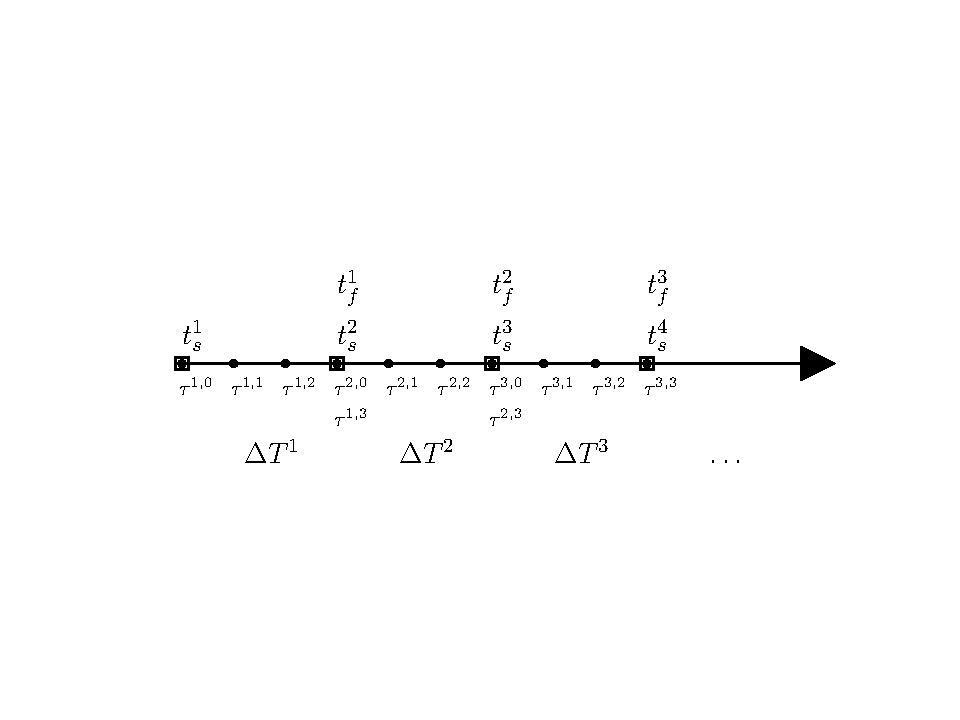
\includegraphics[trim={0.0cm 4.5cm 0cm 3cm},clip,width=1.0\textwidth]{figs/time_grid_timesteps.pdf} 
	\caption{Depiction of the $\nstepsArg{n}+1$ time instances over each window. In the figure, $\nstepsArg{n} = 2$ for all $n$.} 
\label{fig:slab_fig2} 
\end{centering} 
\end{figure}
%We now outline several commonly employed temporal discretization 
%schemes, specifically linear multistep and collocation (Runge--Kutta) methods, that leverage this time-grid to discretize the FOM ODE and 
%objective functional.  

%\subsubsection{Temporal Discretization of the FOM ODE}
%To develop the direct solution approach, we first outline several 
%commonly employed methods used to discretize the FOM ODE, and then 
%subsequently demonstrate how these techniques can be used to discretize 
%and solve Eq.~\ref{eq:obj_gen_slab}. To develop the direct solution approach, 
%we start by dividing each time slab $[\timeStartArg{n},\timeEndArg{n}]$ into
%$\nstepsArg{n}$ strictly increasing time-step instances described by,
%$\{\timeWindowArg{n}{i}\}_{i=0}^{\nstepsArg{n}}$, with  \begin{align*}
%&\timeWindowArg{n}{0} \le \ldots \le \timeWindowArg{n}{\nstepsArg{n}} , \\
%&\timeWindowArg{n}{0} \defeq \timeStartArg{n}, \\
%&\timeWindowArg{n}{\nstepsArg{n}} \defeq \timeEndArg{n}. 
%%\timeWindowArg{n}{0} = \timeStartArg{n}, \timeWindowArg{n}{\nstepsArg{n}} =
%%\timeEndArg{n}
%\end{align*}
\subsubsection{Linear multistep schemes}
Linear multistep schemes approximate the solution at time instance $\timeWindowArg{n}{i}$ using the previous $k$ time instances.  
%Discretizing the FOM ODE~\eqref{eq:FOM} with a linear $k$-step scheme at the $i$th time-instance over the $n$th time slab yields,
%\begin{equation}\label{eq:kstep}
%\sum_{j=0}^{\lmsWidthArg{n}{i}} \alpha_j \stateFOMDiscreteArg{n,i-j} = \Delta t^{n,i} \sum_{j=0}^{\lmsWidthArg{n}{i}} \beta_j \velocity(\stateFOMDiscreteArg{n,i-j}),
%\end{equation}
Employing a linear multistep method to discretize the FOM ODE yields the FOM O$\Delta$E over the $n$th window,
\KTC{Note: the notation here is not consistent with what was defined earlier
for a discrete residual. See email.}
\begin{align*}
&\residLMSArg{n,i} (\stateFOMDiscreteArg{n,i};\stateFOMDiscreteArg{n,i-1},\ldots,\stateFOMDiscreteArg{n,i-\lmsWidthArg{n}{i}}) = \bz, \qquad i=1,\ldots,\nstepsArg{n}, \\
&\stateFOMDiscreteArg{n,0} = \begin{cases}
\stateFOMDiscreteArg{n-1,\nstepsArg{n-1}} & n = 2,\ldots,\nslabs, \\
\stateFOMIC & n=1, \end{cases}
\end{align*}
where $\stateFOMDiscreteArg{n,i} (\approx
\stateFOMArg{}{\timeWindowArg{n}{i}})
\in \RR{\fomdim}$ and $\residLMSArg{n,i}$ denotes the FOM O$\Delta$E
residual over the $i$th time instance of the $n$th window  
defined as
\begin{align*}
\residArg{n,i} &: (\stateyDiscreteArgnt{i};\stateyDiscreteArgnt{i-1},\ldots,\stateyDiscreteArgnt{i-\lmsWidthArg{n}{i}}) \mapsto  \frac{1}{\Delta t^{n,i}} \sum_{j=0}^{\lmsWidthArg{n}{i}} \alpha^{n,i}_j \stateyDiscreteArgnt{i-j} -  \sum_{j=0}^{\lmsWidthArg{n}{i}} \beta^{n,i}_j \velocity(\stateyDiscreteArgnt{i-j},\timeWindowArg{n}{i-j}) \\
               &: \RR{\fomdim} \otimes \RR{\lmsWidthArg{n}{i}+1} \rightarrow \RR{\fomdim}. 
\end{align*} 
Here, $\Delta t^{n,i} \defeq \timeWindowArg{n}{i} - \timeWindowArg{n}{i-1}$
denotes the time step, $\lmsWidthArg{n}{i}$ denotes the number of time steps employed by the scheme at the $i$th time instance over the $n$th window and
$\alpha^{n,i}_j,\beta^{n,i}_j\in\RR{}$ denote coefficients that 
define the specific type of multistep scheme. To handle the case where the linear multistep method employs time instances from the previous window(s), we enforce the condition on the indices $(n,i) = (n-1,\nstepsArg{n-1}+i)$ for $i<0$. 
%\begin{remark}\label{remark:LMS}
%For notational simplicity, we assume the linear multistep method employs time
%	instances from only within the current time window. In general, the linear
%	multistep method at the $n$th window could be designed to employ multiple
%	time instances from previous time windows. \KTC{What are the implications of
%	this? I suggest removing this and adding a simple condition, maybe with a
%	footnote.}
%\end{remark}
%Employing a linear multistep method for temporal discretization of the FOM ODE leads to the FOM O$\Delta$E over the $n$th slab,
%\begin{align*}
%&\residLMSArg{n,i} (\stateFOMDiscreteArg{n,i},\ldots,\stateFOMDiscreteArg{n,i-k^n(i)}) = \bz, \qquad i=1,\ldots,\nstepsArg{n}, \\
%&\stateArgnt{n,0} = \begin{cases}
%\stateFOMDiscreteArg{n-1,\nstepsArg{n-1}} & n = 2,\ldots,\nslabs, \\
%\stateFOMIC & n=1, \end{cases}
%\end{align*}
%where $\residLMSArg{n,i}$ is the discrete linear multistep residual over the $i$th time-step instance of the $n$th slab,
%\begin{align*}
%\residArg{n,i} &: (\stateyDiscreteArgnt{n,i},\ldots,\stateyDiscreteArgnt{n,i-k(i)}) \mapsto  \frac{1}{\Delta t^{n,i}} \sum_{j=0}^{\lmsWidthArg{n}{i}} \alpha_j \stateyDiscreteArgnt{n,i-j} -  \sum_{j=0}^{\lmsWidthArg{n}{i}} \beta_j \velocity(\stateyDiscreteArgnt{n,i-j}),
%\\
%               &: \RR{\fomdim} \otimes \RR{k(i)} \rightarrow \RR{\fomdim}. 
%\end{align*} 
\EP{In the process of reworking this slightly, need to take care for the case where we are employing multiple time steps 
from the previous window. Still cleaning up}
\methodAcronym\ with the direct approach and a linear multistep method sequentially computes the solutions
$\approxstateDiscreteArg{n,1},\ldots,\approxstateDiscreteArg{n,\nstepsArg{n}}$,
$n=1,\ldots,\nslabs$ that satisfy
%	\KTC{What is $\genstate^{n-1}(\timeEndArg{n-1} ) $ doing here? Two problems
%	(1) there is no notion of a generalized coordinate $\genstate$ yet, and (2)
%	this should be the discrete solution, not the exact solution evaluated at
%	the final time.} \EP{You are correct, I think there is an error now in the minimize term though. It was $\in \trialspace\otimes \RR{\lmsWidthArg{n}{i}+1}$, it should be $\trialspace\otimes \RR{\nstepsArg{n}+1}$}
\begin{align*}
	&\underset{(\stateyDiscreteArgnt{1},\ldots,\stateyDiscreteArgnt{\nstepsArg{n}}) \in \trialspace\otimes \RR{\nstepsArg{n}{i}}}{\text{minimize } }
\objectiveArgLMS{n} (\stateyDiscreteArgnt{1},\ldots,\stateyDiscreteArgnt{\nstepsArg{n}}). 
%%& \text{subject to} \hspace{0.2 in}  \stateyDiscreteArg{0} =
%%\begin{cases} \basisspaceArg{n} \spatialICDiscrete + \stateInterceptArg{n}& n = 2,\ldots,\nslabs,\\
%\basisspaceArg{1} \genstateICOne  + \stateInterceptArg{1}& n=1. \end{cases} 
\end{align*}
%Employing a linear multistep method allows the objective \textit{functional}~\eqref{eq:obj} to be replaced with the objective \textit{function}
%\EP{Had to change the definition of the objective function to reflect stepping back into previous window}
In the above, $\objectiveArgLMS{n}$ is the discrete objective function at the $n$th time window and is defined as
\begin{equation}\label{eq:obj_lms}
\begin{split} 
\objectiveArgLMS{n} &\vcentcolon (\stateyDiscreteArgnt{1},\ldots,\stateyDiscreteArgnt{\nstepsArg{n}}) \mapsto
\frac{1}{2} \sum_{i=1}^{\nstepsArg{n}} \quadWeightsLMSScalarArg{n}{i} [\residArg{n,i}(\stateyDiscreteArgnt{i};\ldots, \stateyDiscreteArgnt{i-\lmsWidthArg{n}{i})})]^T  \stweightingMatArgt{n}{\timeWindowArg{n}{i}} \residArg{n,i}(\stateyDiscreteArgnt{i};\ldots, \stateyDiscreteArgnt{i-\lmsWidthArg{n}{i}}), \\
&\vcentcolon \RR{\fomdim} \otimes \RR{\nstepsArg{n}} \rightarrow
\RR{}_+, 
\end{split}
\end{equation}
where $\quadWeightsLMSScalarArg{n}{i} \in \RRplus$ are quadrature weights and, for $i \le 0$ in $\objectiveArgLMS{n}$, we take
\begin{equation}\label{eq:wls_spatial_direct_args}
\stateyDiscreteArgnt{i}  \equiv 
\begin{cases}
\basisspaceArg{n} \basisspaceTArg{n} (\approxstateDiscreteArg{n-1,\nstepsArg{n-1}+i} - \stateInterceptArg{n}) + \stateInterceptArg{n} & n = 2,\ldots,\nslabs,  \\
\basisspaceArg{n} \basisspaceTArg{n} (\stateFOMIC - \stateInterceptArg{n}) + \stateInterceptArg{n} & n = 1.
\end{cases}
\end{equation}
Note that the boundary conditions are automatically satisfied by Eq.~\eqref{eq:wls_spatial_direct_args}.

%where 
%\begin{align*}
%\residArg{n,i} &: (\stateyArgnt{n,i},\ldots,\stateyArgnt{n,i-k(i)}) \mapsto  \sum_{j=0}^k \alpha_j \stateyArgnt{n,i-j} = \Delta t^{n,i} \sum_{j=0}^k \beta_j \velocity(\stateyArgnt{n,i-j}),
%\\
%               &: \RR{\fomdim} \otimes \RR{k(i)} \rightarrow \RR{\fomdim}, 
%\end{align*} 
%is the discrete residual resulting from the linear multistep scheme and 
%\methodAcronym\ solves the minimization problem over each time window, 
%\begin{align*}
%&\approxstateDiscreteArg{n,0},\ldots,\approxstateDiscreteArg{n,\nstepsArg{n}} = \underset{\stateyDiscreteArgnt{n,0},\ldots,\stateyDiscreteArgnt{n,\nstepsArg{n}} \in \trialspace}{\text{arg\,min } }
%\objectiveArgLMS{n} (\stateyDiscreteArgnt{n,0},\ldots,\stateyDiscreteArgnt{n,\nstepsArg{n}}) \\
%& \text{subject to} \hspace{0.2 in}  \approxstateDiscreteArg{n,0} =
%\begin{cases} \approxstateDiscreteArg{n-1,\nstepsArg{n-1}} & n = 2,\ldots,\nslabs,\\
%\approxstateIC & n=1. \end{cases} \end{align*}
	Equivalently, \methodAcronym\ sequentially computes the generalized
	coordinates
	$\genstateDiscreteArg{n,1},\ldots,\genstateDiscreteArg{n,\timeWindowArg{n}{i}}$,
	$n=1,\ldots,\nslabs$ 
with $\genstateDiscreteArg{n,i}(\approx
	\genstateArgnt{n}(\timeWindowArg{n}{i}))\in\RR{\romdim}$
	that satisfy
\begin{equation}\label{eq:obj_gen_lms_final}
\begin{split}
	&
	\underset{(\genstateyDiscreteArg{1},\ldots,\genstateyDiscreteArg{\nstepsArg{n}})\in\RR{\romdim}\otimes \RR{\nstepsArg{n}}}{\text{minimize } }
\objectiveArgLMS{n} (\basisspaceArg{n} \genstateyDiscreteArg{1} + \stateInterceptArg{n},\ldots,\basisspaceArg{n} \genstateyDiscreteArg{\nstepsArg{n}} + \stateInterceptArg{n}). 
%& \text{subject to} \hspace{0.2 in}
%\genstateyDiscreteArg{0} =
%\begin{cases} \genspatialICDiscrete  & n = 2,\ldots,\nslabs \\
%\genstateICOne& n=1. \end{cases} 
\end{split}
\end{equation}
%\begin{equation}\label{eq:obj_gen_lms_final}
%\begin{split}
%& \genstateDiscreteArg{n,0},\ldots,\genstateDiscreteArg{n,\nstepsArg{n}}  = \underset{\genstateyDiscreteArg{n,0},\ldots,\genstateyDiscreteArg{n,\nstepsArg{n}}}{\text{arg\,min } }
%\objectiveArgLMS{n} (\basisspace \genstateyDiscreteArg{n,0} + \stateIntercept,\ldots,\basisspace \genstateyDiscreteArg{n,\nstepsArg{n}} + \stateIntercept) \\ 
%& \text{subject to} \hspace{0.2 in}
%\genstateDiscreteArg{n,0} =
%\begin{cases} \genstateDiscreteArg{n-1, \nstepsArg{n-1}} & n = 2,\ldots,\nslabs \\
%\basisspace^T(\stateFOMIC - \stateIntercept)& n=1. \end{cases} 
%\end{split}
%\end{equation}
The optimization problem takes the form of a \textit{weighted least-squares
	problem}. \KTC{I got rid of (non)linear. If it's either linear or nonlinear,
	then omit it as an adjective, as this is no longer descriptive. }
We emphasize that optimization problem~\eqref{eq:obj_gen_lms_final} associates
	with an \spatialAcronym\ trial subspace characterized by a reduction in
	spatial complexity, but no reduction in temporal complexity.
 
The minimization problem~\eqref{eq:obj_gen_lms_final} requires specification of the quadrature weights (and hence the integration scheme used to discretize 
the objective functional). Typically, the same integration scheme used to discretize the FOM ODE is employed for consistency~\cite{colloc_review}; e.g., if a  
backward Euler method is used to discretize the FOM ODE, then a backward Euler method is the used to numerically integrate the objective functional.

\begin{remark}
For the limiting case where $\nstepsArg{n} = 1$ such that the window size is equivalent to the time step, $\DeltaSlabArg{n} \equiv \timeWindowArg{n}{1} - \timeWindowArg{n}{0}$, uniform 
quadrature weights are used, and uniform bases and weighting matrices are used, 
\methodAcronym\ with \spatialAcronym\ trial
	subspaces solved via the direct approach recovers LSPG. \KTC{Not exactly. To
	make this LSPG as presented earlier, also require the time grid here to
	align with the time grid used for time integration earlier. Also, this
	formulation requires allowing the stencil to go back to time steps at
	previous windows.} \EP{I agree with the second comment, to be 100\% precise we need to go back into other time windows. Clearly you can do this if you would like, and I think the comment clarifies this. Hopefully can avoid this now with the condition you mentioned. I think the first comment is not required. The LSPG ``approach" minimizes the residual at a time instance; it isn't tied to the description we gave earlier.} 
\end{remark} 
\subsubsection{Solution to the least-squares problem through the Gauss--Newton method}
	\KTC{If the dynamics are linear, doesn't this just yield a linear
	least-squares problem that can be solved directly? We need to present this
	more clearly.}
Discretization through linear multistep methods (as well as other techniques) 
results in a (non)linear least-squares problem.
A variety of algorithms exist for solving least-squares problems, including trust region approaches, the Gauss–Newton method, and the Levenberg–Marquardt method.  
The numerical experiments presented in this work consider the Gauss--Newton method, and as such we outline this approach here. 

To describe the Gauss--Newton method, we first define a ``vectorization" function 
\begin{align*}
 \unroll &\vcentcolon (\stateyDiscreteArg{1},\ldots,\stateyDiscreteArg{m} ) \mapsto \begin{bmatrix} [\stateyDiscreteArg{1}]^T & \ldots & [\stateyDiscreteArg{m}]^T \end{bmatrix}^T  \\
&\vcentcolon \RR{p} \otimes \RR{m} \rightarrow \RR{pm}.
\end{align*}
The vectorized generalized coordinates over the $n$th time window are then
defined as \KTC{notationally, why are we doing a double bar instead of a bar?}
\EP{The notation for space--time in 2.4 uses bars. I don't want to confuse these generalized coordinates with those, they conceptually two different things} 
\begin{equation*}
\genstatecollocMatSlabArg{n} \defeq 
\unroll (\genstateDiscreteArg{n,1},\ldots,\genstateDiscreteArg{n,\nstepsArg{n}} ).
\end{equation*}
We now define the weighted space--time residual over the entire window as
\KTC{To make this valid for seeping back into the previous time window, the
second argument could be omitted here (okay because there is already a
superscript on the residual) and arbitrary previous solutions could be
included in the first residual here.}
\begin{equation*}
\residLMSSlabArg{n} : (\genstatecollocMatySlabArg{};\genstateDiscreteArg{n,0}) \mapsto \begin{bmatrix}
 \sqrt{\quadWeightsLMSScalarArg{n}{1} } \stweightingMatOneArg{n} \residLMSArg{n,1}( \basisspaceArg{n} \genstateyDiscreteArgnt{1} + \stateInterceptArg{n},  \basisspaceArg{n} \genstateDiscreteArg{n,0} + \stateInterceptArg{n},) \\
\vdots \\
 \sqrt{\quadWeightsLMSScalarArg{n}{\nstepsArg{n}} } \stweightingMatOneArg{n} \residLMSArg{n,\nstepsArg{n}}( \basisspaceArg{n} \genstateyDiscreteArgnt{\nstepsArg{n}} + \stateInterceptArg{n}, \ldots,\basisspaceArg{n} \genstateyDiscreteArgnt{\nstepsArg{n} - k^n(\nstepsArg{n}) } + \stateInterceptArg{n}) \\
\end{bmatrix},
\end{equation*}
where $\genstatecollocMatySlabArg{} \defeq \unroll (\genstateyDiscreteArg{1},\ldots,\genstateyDiscreteArg{\nstepsArg{n}} ).$
It is worth noting that, by design, \KTC{This is incorrect. Missing a 1/2
factor}
\begin{equation*}
\objectiveArgLMS{n} \bigg( \basisspaceArg{n} \genstateDiscreteArg{n,0} + \stateInterceptArg{n},\ldots,\basisspaceArg{n} \genstateDiscreteArg{n,\nstepsArg{n}} + \stateInterceptArg{n} \ \bigg) 
=
\bigg[\residLMSSlabArg{n}  (\genstatecollocMatSlabArg{n};\genstateDiscreteArg{n,0}) \bigg]^T \bigg[ \residLMSSlabArg{n}(\genstatecollocMatSlabArg{n};\genstateDiscreteArg{n,0}) \bigg].
\end{equation*} 
Using these definitions, Algorithm~\ref{alg:colloc_gn} presents the standard Gauss--Newton method. The algorithm consists of three fundamental steps: (1) compute the FOM O$\Delta$E residual given the current guess, (2) compute the Jacobian of the residual over the time window and form the normal equations, and (3) solve the normal equations and update the state. 

The practical implementation of the Gauss--Newton algorithm requires an efficient method for computing the Jacobian of the residual over the time window. In particular, it is important to note that for linear multistep methods (and many other time marching schemes) the Jacobian of the residual over the time window will an almost block-diagonal 
sparse matrix with the sparsity pattern \KTC{number of residual arguments
inconsistent with above}
\begin{equation*}
\frac{\partial \residLMSSlabArg{n}}{\partial \genstatecollocMatySlabArg{}}(\genstatecollocMatSlabArg{n})  =
 \begin{bmatrix*}[l]
\matshapeb & \\%[-5pt]
 \matshapea & \matshapea & \\%[-5pt]
 & \matshapea  & \matshapea & \\%[-5pt]
&  & \ddots & \\%[-5pt]
 & &  & \matshapea &  \matshapea 
\end{bmatrix*}.
% \begin{bmatrix*}[c]
%\matshapeb & \\[-5pt]
% & \hspace{-12pt}\matshapea & \\[-5pt]
% &  & \hspace{-12pt}\matshapea & \\[-5pt]
%&  & \hspace{5pt} \ddots & \\[-5pt]
% & &  & & \hspace{-15 pt} \matshapea 
%\end{bmatrix*}.
\end{equation*}
This sparsity pattern can be leveraged to assemble the Jacobian of the residual over the time window from Jacobians of the residual at single time instances. 
Further, the sparsity pattern can be 
leveraged \KTC{split infinitive:} to efficiently compute the Jacobian
\KTC{shoudl be an en-dash:} matrix-matrix product in the normal equations.
\KTC{We should never be solving the normal equations. This squares the
condition number!}
It is also worth noting that the 
normal equations will also (almost) \KTC{What does ``almost'' block diagonal
mean? This is imprecise} be block-diagonal; this is a fact that can be leveraged to speed up the linear solves at each Gauss--Newton iteration.

\begin{remark}\label{remark:gaussnewton}\textit{(Acceleration of the Gauss--Newton Solve)}\\
	The \KTC{this should be `principal', not `principle':} principle cost of a Gauss--Newton method is often the formation of the Jacobian matrix. A variety of techniques aimed at 
reducing this computational burden exist; Jacobian-free Newton-Krylov
	methods~\cite{jfnk}, Broyden's method~\cite{broyden} (as explored in
	Ref.~\cite{carlberg_thesis}, Appendix A), and frozen Jacobian approximations
	are several such examples. \KTC{Expose used twice in this sentence} Further, the space--time formulation exposes an extra dimension for parallelization that can be exposed to accelerate the wall-clock time of the ROM. The investigation of these additional, potentially more efficient, solution algorithms will be a topic of future work. 
\end{remark}
%\subsubsection{Jacobian-Free Implementation}
%The dominant cost of the Gauss Newton algorithm is the computatation of the action of the Jacobian matrix on the trial basis. To alleviate this burden, the following Jacobian-free method is proposed:
\begin{algorithm}
\caption{\spatialAcronym\ trial subspace: algorithm for the direct solution technique with the Gauss--Newton method and a linear multistep method over the $n$th window}
\label{alg:colloc_gn}
\SetKwInOut{Input}{Input}\SetKwInOut{Output}{Output}
\Input{tolerance, $\epsilon$; initial guess, $\genstateGuessDiscreteArg{n,1}{0},\ldots,\genstateGuessDiscreteArg{n,\nstepsArg{n}}{0}$; initial condition $\genstateDiscreteArg{n,0}$}
\Output{Solution to least squares problem, $\genstatecollocMatSlabArg{n}$} 
\textbf{Online Steps}: \\
$\text{converged} \leftarrow \text{false}$ \Comment{Set convergence checker} \\
$k \leftarrow 0$ \Comment{Set counter}\\
$\genstatecollocMatSlabArg{n}_k \leftarrow \unroll(\genstateGuessDiscreteArg{n,1}{0},\ldots,\genstateGuessDiscreteArg{n,\nstepsArg{n}}{0})$ \Comment{Assemble generalized coordinates over window} \\
\While{\text{converged} == \text{false}}
{
%\For{$i=1,\hdots,\nstepsArg{n}$}{
%  \For{$j=1,\hdots,\ncollocArg{n}{i}$}{
%Compute: $\approxstateArgnt{n,i}  =  \basisspace  \genstateDiscreteArg{n,i} + \stateIntercept$ 
%\Comment{Compute state} \\
%Compute: $\velocity(\basisspace \genstateDiscreteArg{n,i} + \stateIntercept ) $ \Comment{Compute velocity at each time-step instance}\\
%Compute: $\residLMSArg{n,i}(\basisspace \genstateDiscreteArg{n,i} + \stateIntercept, \ldots , \basisspace \genstateDiscreteArg{n,i - k^n(i)} + \stateIntercept) $  \Comment{Compute residual} \\
%}
$\mathbf{r} \leftarrow \residLMSSlabArg{n}(\genstatecollocMatSlabArg{n}_k;\genstateDiscreteArg{n,0})$ \Comment{Compute weighted residual over window} \\
$\mathbf{J} \leftarrow  
\frac{\partial \residLMSSlabArg{n}}{\partial \genstatecollocMatySlabArg{}}(\genstatecollocMatSlabArg{n}_k) 
$ \Comment{Compute weighted residual-Jacobian over window} \\
%Compute: $[\jacobianSlabArg{n}]^T \jacobianSlabArg{n}$ \Comment{Compute system matrix for the normal equations} \\
%Compute: $[\jacobianSlabArg{n}]^T \residLMSSlabArg{n}(\genstatecollocMatSlabArg{n}_k)$ \Comment{compute RHS for normal equations} \\
 Compute  $\Delta  \genstatecollocMatSlabArg{n} $ satisfying $ [\mathbf{J}]^T \mathbf{J} \Delta \genstatecollocMatSlabArg{n}=  -\mathbf{J}^T\mathbf{r}$ \Comment{Solve the normal equations} \\
$\genstatecollocMatSlabArg{n}_{k+1} \leftarrow \genstatecollocMatSlabArg{n}_k + \Delta \genstatecollocMatSlabArg{n}$ \Comment{Update guess to the state} \\
\If{ $\norm{ \mathbf{J}^T\mathbf{r}  } \le \epsilon$ }{
{\text{converged} $\leftarrow$ \text{true}}  \Comment{Check and set convergence based on gradient norm} \\
Return: $\genstatecollocMatSlabArg{n} = \genstatecollocMatSlabArg{n}_{k+1} $ \Comment{Return converged solution}\\
}
$k\leftarrow k+1$
}
\end{algorithm}


%\input{direct_collocation}

\subsection{\spatialAcronym\ trial subspaces: indirect solution approach}\label{sec:indirect}
In contrast to the direct approach,
indirect methods ``indirectly" solve the minimization
problem~\eqref{eq:tclsrm} by solving the Euler--Lagrange equations. The
system given by the Euler--Lagrange equations~\eqref{eq:lspg_continuous}--\eqref{eq:lspg_adjoint} comprises a coupled two-point boundary value
problem. A variety of techniques have
been devised to solve two-point boundary value problems of this type. These
techniques include shooting methods, multiple shooting
methods~\cite{multiple_shooting}, and the forward--backward sweep
method~\cite{fbs} (FBSM).  This work explores using the FBSM. 

%Solving this coupled problem is significantly more challenging and
%computationally expensive than the standard Galerkin and LSPG methods as it
%requires converging both the forward and backward solve. It is emphasized,
%however, that the entire forward-backward system is compatable with
%hyper-reduction techniques and thus is entirely independent of the full-order
%model size. In addition, as the approach is minimizing the entire space-time
%residual, we expect it to be capable of providing stable and accurate
%solutions in cases where the standard Galerkin and LSPG methods can not.
%Obtaining numerical solutions to Eq.~\ref{eq:lspg_continuous} requires three
%ingrediants: \begin{enumerate} \item Solution strategy for solving the
%coupled forward and backwards problems \item Time discretization schemes for
%the forward and backward problems \item Efficient strategy for evaluating the
%action of the Jacobian transpose on a vector \end{enumerate}

\subsubsection{Forward--backward sweep method (FBSM)}\label{sec:FBSM}
%\subsubsection{Solution Strategy} Solving Eq.~\ref{eq:lspg_continuous} is
%made challenging by the fact that it is a coupled two-point boundary value
%problem. The forward problem is coupled to the backwards adjoint problem,
%while the backwards adjoint sytem is coupled to the forward problem. The
%problem is thus inherently implicit. The most popular techniques to solve
%these types of two-point boundary value problems are shooting methods,
%multiple shooting methods, fully-implicit methods, and the forward backward
%sweep (FBS) method. This work explores using the FBS method. 

%The most straightforward approach to solving Eq.~\ref{eq:lspg_continuous} is
%to 1.) discretized both the forward and backwards problems in time and 2.)
%form and solve the resulting (implicit) nonlinear space-time system. In
%practice, however, this technique may not be practical for larger
%time-windows due to the size of the resuling nonlinear problem. 

The FBSM is an iterative approach that can be used to
solve the two-point boundary value problem. The general process of the FBSM is
as follows: First, the system~\eqref{eq:lspg_continuous} is (numerically) solved forward in
time using an initial guess to the costate to obtain an initial guess to
the generalized coordinates. Next, the adjoint equation~\eqref{eq:lspg_adjoint} is solved \textit{backwards} in time given the
approximation to the generalized coordinates. This gives a new estimate to the
costate, which is then used to again solve the forward problem to obtain
a new estimate of the generalized coordinates. This process is continued until
convergence. Algorithm~\ref{alg:st_iter} outlines the method. The algorithm
contains three parameters: the damping factor $\rho \le 1$, the growth factor
$\fbsmGrowth \ge 1$, and the decay factor $\fbsmDecay \ge 1$. The damping factor controls the rate at which the costate seen by~\eqref{eq:lspg_continuous} is updated. The
closer $\rho$ is to unity, the faster the resulting algorithm will converge.
For large window sizes, however, too high a value of $\rho$ can lead to an unstable iterative process. 
A proper value of $\rho$ can be
obtained with a line search. The line search presented in Algorithm~\ref{alg:st_iter} adapts the damping factor
according to the objective. Convergence properties of the FBSM method are
presented in Ref.~\cite{McAsey2012ConvergenceOT}. It is shown that, for a small 
enough value of $\rho$, the algorithm will converge.

\begin{algorithm} \caption{\spatialAcronym\ trial subspace: algorithm for the FBSM over the $n$th window.} \label{alg:st_iter} 
\SetKwInOut{Input}{Input}\SetKwInOut{Output}{Output}
\Input{tolerance, $\epsilon$; damping factor, $\rho \le 1$; growth factor, $\fbsmGrowth \ge 1$; decay
factor, $\fbsmDecay \ge 1$} 
\Output{Stationary point, $\genstateArgnt{n}$ }
\textbf{Online Steps:}\\ 
$\genstate^n_0 \leftarrow \bz$ \Comment{Set initial guess for state} \\
$\controllerArgnt{n} \leftarrow \boldsymbol 0$ \Comment{Set initial
guess for costate}\\ 
$\text{Compute } \genstateArgnt{n}_1 \text{ satisfying } \basisspaceTArg{n} \stweightingMatArg{n}
\basisspaceArg{n} \genstateDotArgnt{n}_1(t)  -  \basisspaceTArg{n} \stweightingMatArg{n}
\velocity(\veloargsromArg{1}) =  \controllerArg{n}{t}$ 
% Eq.~\ref{eq:lspg_continuous} with $\adjoint^n(t) = \controllerArg{n}{t}$ to
% obtain $\genstate_0^{n}(t)$ 
\Comment{Solve~\eqref{eq:lspg_continuous}}\\ 
%Set: $\genstate^n_1 = \genstate$ \Comment{Set state} \\
%$\objectiveArg{n}({\genstate_1^n(t)})$
%\Comment{Evaluate objective function}\\
$i \leftarrow 1$ \Comment{Set counter}\\
\While{$\epsilon \le \int_{\timeStartArg{n}}^{\timeEndArg{n}} \norm{\genstate^n_{i}(t) - \genstate^n_{i-1}(t) }dt $}{
\small{
\begin{multline*}
\text{ Compute } \adjointArgnt{n} \text{ satisfying }
\adjointDotArg{n}{t}  + \basisspaceTArg{n} \bigg[\frac{\partial \velocity}{\partial \stateyDiscrete}(\basisspaceArg{n} \genstate^n_i(t) + \stateInterceptArg{n},t) \bigg]^T \stweightingMatArg{n} \basisspaceArg{n} [\massArg{n}]^{-1} \adjointArg{n}{t}= \\ -\bigg[\basisspaceTArg{n} \bigg[ \frac{\partial \velocity}{\partial \stateyDiscrete} ( \basisspaceArg{n} \genstate^n_i(t) + \stateInterceptArg{n},t) \bigg]^T \stweightingMatArg{n} \bigg( \mathbf{I} -   \basisspaceArg{n} [\massArg{n}]^{-1} \basisspaceTArg{n} \stweightingMatArg{n} \bigg)  \bigg( \basisspaceArg{n} \dot{\genstate}_i^n(t)   -   \velocity( \basisspaceArg{n} \genstate_i^n(t)  +\stateInterceptArg{n},t) \bigg) \bigg] 
\end{multline*} }
\Comment{Solve~\eqref{eq:lspg_adjoint} to obtain guess to costate} \\
%Solve Eq.~\ref{eq:lspg_adjoint} with $\genstate^n(t) = \genstate^n_i(t)$ to obtain $\adjoint^n(t)$ \\
$\controllerArgnt{n}  \leftarrow \rho \controllerArgnt{n} + (1 - \rho) \adjointArgnt{n}$ \Comment{Weighted update to costate}\\
$i \leftarrow i+1$ \Comment{Update counter}\\
$\text{Compute }\genstateArgnt{n}_i \text{ satisfying } \basisspaceTArg{n} \stweightingMatArg{n} \basisspaceArg{n} \genstateDotArgnt{n}_i(t)   -  \basisspaceTArg{n} \stweightingMatArg{n} \velocity(\basisspaceArg{n} \genstate^n_i(t) + \stateInterceptArg{n},t) =  \controllerArg{n}{t} $
\Comment{Solve~\eqref{eq:lspg_continuous}}\\
%$\objectiveArg{n}({\genstate_i^n(t)})$ \Comment{Evaluate objective function}\\
\uIf{ $\objectiveArg{n}({\basisspaceArg{n}\genstate_i^n + \stateInterceptArg{n}\otimes \onesFunctionArg{n}}) \le \objectiveArg{n}({\basisspaceArg{n}\genstate_{i-1}^n + \stateInterceptArg{n}\otimes \onesFunctionArg{n}})$}
{
$\rho \leftarrow \text{min}(\rho \fbsmGrowth,1)$ \Comment{Grow the damping factor}\\
}
\Else{
$\rho \leftarrow \frac{\rho }{ \fbsmDecay}$ \Comment{Shrink the damping factor}\\ 
$\genstate_i^{n} \leftarrow  \genstate_{i-1}^{n}$ \Comment{Reset state to value at previous iteration}
}
}
Return converged solution, $\genstateArgnt{n}= \genstateArgnt{n}_i$
\end{algorithm}
\subsubsection{Numerical considerations for the forward and backward problems}
The FBSM requires solving the systems~\eqref{eq:lspg_continuous} and~\eqref{eq:lspg_adjoint}, both of which are defined at the time-continuous level. 
The numerical implementation of the FBSM requires two main ingredients: (1) temporal discretization schemes for the forward and backward problems and (2) 
an efficient method for computing the action of the Jacobian transpose on a vector.  

This work examines the use of linear multistep methods for the purpose of temporal discretization of the forward and 
backwards problems. As described in  
the direct solution approach, temporal discretization is achieved by introducing $\nstepsArg{n} + 1$ time instances~\eqref{eq:timegrid1} over each time window. Linear multistep methods then use this time-grid for temporal discretization of~\eqref{eq:lspg_continuous} and~\eqref{eq:lspg_adjoint}. 

The second ingredient, namely an efficient method for computing the action of the Jacobian transpose on a vector, can be challenging. 
In the case one does not have access to the full-order model Jacobian (or it is too costly to compute), the evaluation of this term can be both challenging and expensive. Here, two methods are discussed that can be used to evaluate the action of the Jacobian transpose on a vector as seen in~\eqref{eq:lspg_adjoint}:
\begin{enumerate}
\item \textit{Jacobian-free approximation}: A non-intrusive way to evaluate the Jacobian transpose in~\eqref{eq:lspg_adjoint} is to recognize that all terms including the Jacobian transpose are left multiplied by the transpose of the trial basis. One can make the manipulation,
$$\basisspaceTArg{n} \bigg[\frac{\partial \velocity}{\partial \stateyDiscrete} (\veloargsromn)\bigg]^T = \bigg[  \frac{\partial \velocity}{\partial \stateyDiscrete} (\veloargsromn) \basisspaceArg{n} \bigg]^T.$$
This manipulation allows one to compute the action of the Jacobian on each column of $\basisspaceArg{n}$ by, e.g., the finite difference approximation
$$\frac{\partial \velocity}{\partial \stateyDiscrete}(\veloargsromn) \basisvec_i^n \approx \frac{1}{\epsilon}\bigg( \velocity(\basisspaceArg{n}\genstateArg{n}{t} + \stateInterceptArg{n} + \epsilon \basisvec_i^n,t) - \velocity(\veloargsromn) \bigg).$$
The Jacobian transpose can be formed in $K+1$ evaluations of the velocity. For cases where the reduced-order model is low dimensional, this approach is feasible. For higher dimensional reduced-order models, this approach can be prohibitively expensive.

\item \textit{Automatic differentiation}: A more intrusive, but potentially more efficient, method of computing the action of the Jacobian transpose on a vector is through automatic differentiation (AD). AD methods comprise a class of techniques that can be used to numerically evaluate derivatives of functions (e.g., Jacobians, vector-Jacobian products) by recursively applying the chain rule. The numerical examples presented later in this work leverage AD. The principle drawback of AD is that AD methods are intrusive and may not be suitable for, e.g., legacy codes.  
\end{enumerate}

\begin{remark}\label{remark:fbsm}(Acceleration of Indirect Methods)
The FBSM is a simple iterative method for solving the coupled two-point boundary value problem. For large time windows, however, the FBSM may require many 
forward--backward iterations for convergence. More sophisticated solution techniques, such as a multiple FBSM method or multiple shooting methods, promise 
to reduce this cost. Analyses of additional solution techniques will be a subject of future work.
\end{remark}


\subsection{\spaceTimeAcronym\ trial spaces: direct and indirect methods}
We now briefly consider \spaceTimeAcronym\ trial subspaces. 
For \spaceTimeAcronym\ trial subspaces, the distinction between a direct and indirect method is less clear as the optimization variable (i.e., the generalized coordinates) are finite 
dimensional. There is no need to transcribe an infinite dimensional optimization variable into a finite dimensional one. There is, however, still a need to develop a finite 
dimensional representation of the objective functional~\eqref{eq:obj_gen_slab}. In what follows, we describe two techniques to do this: one that works with the FOM O$\Delta$E and one that works with the FOM ODE. We associate direct methods as those 
that work with the O$\Delta$E and indirect methods with those that work directly with the ODE.  

\subsection{\spaceTimeAcronym: direct solution approach}
The direct solution technique seeks to minimize the fully discrete objective function associated with the O$\Delta$E. For brevity, we again focus on linear multistep methods and leverage the time grids introduced in Section~\ref{sec:direct}. For notational simplicity, we define an index mapping function that is 
equivalent to the mapping function $\indexMapper$, but outputs only the first argument: 
$$\indexMappern: (n,i) \mapsto 
\begin{cases}
n & n = 1, \; i = 0, \\
n & n \ge 1, \; i > 0, \\
\indexMappern(n-1,\nstepsArg{n-1}+i) & n > 1, \; i \le 0.
\end{cases}$$
%The definition of the fully discrete objective functions~\eqref{eq:obj_lms} as outlined in Section~\ref{sec:direct}, can be leveraged for this purpose. For simplicity, we only 
%outline the case for linear multistep schemes. 
Assuming $\text{Rank}(\stweightingMatOneArg{n})\nstepsArg{n} \ge \stdimArg{n}$, \methodAcronym\ with the direct approach and an \spaceTimeAcronym\ trial subspace sequentially computes the generalized coordinates $\stgenstateArg{n}$, $n=1,\ldots,\nslabs$ that satisfy
 \begin{equation}\label{eq:obj_gen_lms_final_st}
\begin{split}
& \underset{\stgenstatey \in \RR{\stdimArg{n}}}{\text{minimize } }
\objectiveArgLMS{n}_{\text{D-ST}} (\stbasisArg{n}{\timeWindowArg{n}{1}} \stgenstatey + \stateInterceptSTArg{n},\ldots,\stbasisArg{n}{\timeWindowArg{n}{\nstepsArg{n}}} \stgenstatey + \stateInterceptSTArg{n}),%  \\
%&\text{subject to } \;  \stbasisArg{n}{\timeStartArg{n}}\stgenstateyArg{n} = \begin{cases} 
%\mathbb{P}^n(\stbasisArgnt{n-1}\stgenstateArg{n-1})(\timeEndArg{n-1}) & n = 2,\ldots,\nslabs, \\ 
%\mathbb{P}^n(\stateFOMArgnt{1})(0) &
%n=1. \end{cases}
\end{split} 
\end{equation}
where the space--time objective function for the direct method is
$$
\objectiveArgLMS{n}_{\text{D-ST}}  :  (\stateyDiscreteArgnt{1},\ldots,\stateyDiscreteArgnt{\nstepsArg{n}}) \mapsto \objectiveArgLMS{n}_{\text{D}}(\stateyDiscreteArgnt{1},\ldots,\stateyDiscreteArgnt{\nstepsArg{n}}; \approxstateArg{\indexMappern(n,0)}{\timeWindow^{\indexMapper(n,0)}},\ldots, 
 \approxstateArg{\indexMappern(n,-\lmsWidthArg{n}{1}+1)}{\timeWindow^{\indexMapper(n,-\lmsWidthArg{n}{1}+1)}}).
$$
It is noted that the boundary conditions are automatically satisfied through the definition of the \spaceTimeAcronym\ trial subspace. The minimization problem~\eqref{eq:obj_gen_lms_final_st} again yields a least-squares problem.
\begin{remark}
For the limiting case where one window comprises entire domain (i.e., $\DeltaSlabArg{1}\equiv T$), uniform quadrature weights are used, the trial space is set to be $\stspaceSTArg{1} = \stspaceST$, the weighting matrices $\stweightingMatArg{1}$ and $\lspgWeightingST$ comprise the identity matrix $\mathbf{I}$, and $\nstepsArg{1} = N_t$ time instances are employed that satisfy $\timeWindowArg{1}{i} = t^i$, $i=1,\ldots,N_t$, then $\stgenstateArg{1} =  \stgenstate_\text{ST-LSPG}$ and direct \methodAcronym\ with an \spaceTimeAcronym\ trial subspace recovers ST-LSPG. 
\end{remark}

\begin{remark}
To enable equivalence in the case for general $\lspgWeightingSTArg{\cdot}$, the weighting matrix $\stweightingMatArg{1}$ needs to be a time-dependent matrix function such that the objective function~\eqref{eq:obj_gen_lms_final_st} permits a modified space--time norm. This is not pursued here.
\end{remark}
 
%\EP{I will rework this section depending on 4.2\\
%Leveraging the definition of the fully discrete objective function~\eqref{eq:obj_lms}, and assuming $N \nstepsArg{n} \ge \stdimArg{n}$, \methodAcronym\ leveraging a \spaceTimeAcronym\ basis sequentially computes the generalized coordinates $\stgenstateArg{n}$, $n=1,\ldots,\nslabs$, that satisfy
% \begin{equation}\label{eq:obj_gen_lms_final_st}
%\begin{split}
%& \underset{\stgenstatey}{\text{minimize } }
%\objectiveArgLMS{n} (\stbasisArg{n}{\timeWindowArg{n}{0}} \stgenstatey + \stateInterceptSTArg{n},\ldots,\stbasisArg{n}{\timeWindowArg{n}{\nstepsArg{n}}} \stgenstatey + \stateInterceptSTArg{n}).%  \\
%%&\text{subject to } \;  \stbasisArg{n}{\timeStartArg{n}}\stgenstateyArg{n} = \begin{cases} 
%%\mathbb{P}^n(\stbasisArgnt{n-1}\stgenstateArg{n-1})(\timeEndArg{n-1}) & n = 2,\ldots,\nslabs, \\ 
%%\mathbb{P}^n(\stateFOMArgnt{1})(0) &
%%n=1. \end{cases}
%\end{split} 
%\end{equation}
%% \begin{equation}\label{eq:obj_gen_lms_final_st}
%%\begin{split}
%%&\stgenstateArg{n} = \underset{\stgenstatey}{\text{arg\,min } }
%%\objectiveArgLMS{n} (\stbasisArg{n}{\timeWindowArg{n}{0}} \stgenstatey + \stateInterceptArg{n},\ldots,\stbasisArg{n}{\timeWindowArg{n}{\nstepsArg{n}}} \stgenstatey + \stateInterceptArg{n})  \\
%%&\text{subject to } \;  \stbasisArg{n}{\timeStartArg{n}}\stgenstateArg{n} = \begin{cases} 
%%\mathbb{P}^n(\stbasisArgnt{n-1}\stgenstateArg{n-1})(\timeEndArg{n-1}) & n = 2,\ldots,\nslabs, \\ 
%%\mathbb{P}^n(\stateFOMArgnt{1})(0) &
%%n=1. \end{cases}\end{split} 
%%\end{equation}
%It is noted that the boundary conditions are automatically satisfied through the definition of the \spaceTimeAcronym\ trial subspace. The minimization problem~\eqref{eq:obj_gen_lms_final_st} can be solved, e.g, via the Gauss--Newton method.
%
%\begin{remark}
%For the limiting case where the window size spans the entire domain, $\DeltaSlabArg{1}\equiv T$, and uniform quadrature weights are used, and the weighting matrix $\stweightingMatArg{n} = \mathbf{I}$, direct \methodAcronym\ with a \spaceTimeAcronym\ trial subspace recovers ST-LSPG with $\lspgWeightingSTArg{\cdot} = \mathbf{I}$. For equivalence conditions in the case where $\lspgWeightingSTArg{\cdot} \ne \mathbf{I}$, the objective function~\eqref{eq:obj_gen_lms_final_st} can be modified to enable weighted space--time norm. 
%\end{remark}
%}
\subsection{\spaceTimeAcronym: indirect solution approach}
As opposed to the direct approach, the indirect approach directly minimizes the continuous objective function~\eqref{eq:obj_gen_slab_spacetime} and sequentially computes solutions $\stgenstateArg{n}$, $n = 1,\ldots,\nslabs$ that satisfy
\begin{equation}\label{eq:obj_gen_slab2}
\begin{split}
 & \underset{\stgenstatey \in \RR{\stdimArg{n}}}{\text{minimize }} \mathcal{J}^n \bigg( \stbasisArgnt{n} \stgenstatey + \stateInterceptSTArg{n} \otimes \onesFunctionArg{n} \bigg) .%\\  
%&\text{subject to } \;  \stbasisArg{n}{\timeStartArg{n}}\stgenstateyArg{n} = \begin{cases} 
%\mathbb{P}^n(\stbasisArgnt{n-1}\stgenstateArg{n-1})(\timeEndArg{n-1}) & n = 2,\ldots,\nslabs, \\ 
%\mathbb{P}^n(\stateFOMArgnt{1})(0) &
%n=1. \end{cases} 
\end{split} 
\end{equation}
%\begin{equation}\label{eq:obj_gen_slab2}
%\begin{split}
% &\stgenstate^n =
%\underset{\stgenstatey}{\text{arg\,min }} \mathcal{J}^n \bigg( \stbasisArgnt{n} \stgenstatey + \stateInterceptArg{n}  \bigg) \\  
%&\text{subject to } \;  \stbasisArg{n}{\timeStartArg{n}}\stgenstateArg{n} = \begin{cases} 
%\mathbb{P}^n(\stbasisArgnt{n-1}\stgenstateArg{n-1})(\timeEndArg{n-1}) & n = 2,\ldots,\nslabs, \\ 
%\mathbb{P}^n(\stateFOMArgnt{1})(0) &
%n=1. \end{cases} 
%\end{split} 
%\end{equation}
%The first order optimality conditions are given by,
%\begin{equation}\label{eq:st_stationary}
% \intSlabArg{n} \bigg[ \stbasisDotArg{n}{t}^T  - \stbasisArg{n}{t}^T \bigg[\frac{\partial
%\velocity}{\partial \stateyDiscrete} (\stbasisDotArg{n}{t} \stgenstateArg{n} +                    
%\stateInterceptArg{n})\bigg]^T  \bigg] \stweightingMatArg{n} \bigg( \stbasisDotArg{n}{t} \stgenstateArg{n}  - \velocity (\stbasisArg{n}{t} \stgenstateArg{n} + \stateInterceptArg{n}) \bigg) dt = \bz.\end{equation}
Numerically solving the minimization problem requires the introduction of a quadrature rule for 
discretization of the integral. Towards this end we introduce $\ncollocSTArg{n} \ge \text{ceil}(\stdimArg{n}/ \text{Rank}(\stweightingMatOneArg{n}))$ quadrature points over the $n$th window, $ \{ \collocPointSTArg{n}{i} \}_{i=1}^{\ncollocSTArg{n}} \subset [\timeStartArg{n},\timeEndArg{n}]$, $n=1,\ldots,\nslabs$. 
%with $\timeStartArg{n} \le \collocPointSTArg{n}{1} \le \cdots \le \collocPointSTArg{n}{\ncollocSTArg{n}} \le \timeEndArg{n}.$
Leveraging these quadrature points, \methodAcronym\ with the indirect method and an \spaceTimeAcronym\ trial subspace computes the generalized coordinates 
$\stgenstateArg{n}$, $n=1,\ldots,\nslabs$ that satisfy
\begin{equation}\label{eq:obj_gen_slab2} 
\begin{split}
&\underset{\stgenstatey \in \RR{\stdimArg{n}}}{\text{minimize }} \objectiveDiscreteSTArg{n} \bigg( \stbasisArgnt{n} \stgenstatey + \stateInterceptSTArg{n} \otimes \onesFunctionArg{n}  \bigg) , %\\
%&\text{subject to }\;  \stbasisArg{n}{\timeStartArg{n}}\stgenstateyArg{n} = \begin{cases} 
%\mathbb{P}^n(\stbasisArgnt{n-1}\stgenstateArg{n-1})(\timeEndArg{n-1}) & n = 2,\ldots,\nslabs, \\ 
%\mathbb{P}^n(\stateFOMArgnt{1})(0) &
%n=1,
%\end{cases}
\end{split} 
\end{equation}
%\begin{equation}\label{eq:obj_gen_slab2} 
%\begin{split}&\stgenstate^n =
%\underset{\stgenstatey}{\text{arg\,min }} \objectiveDiscreteSTArg{n} \bigg( \stbasisArgnt{n} \stgenstatey + \stateInterceptArg{n}  \bigg) , \\
%&\text{subject to }\;  \stbasisArg{n}{\timeStartArg{n}}\stgenstateArg{n} = \begin{cases} 
%\mathbb{P}^n(\stbasisArgnt{n-1}\stgenstateArg{n-1})(\timeEndArg{n-1}) & n = 2,\ldots,\nslabs, \\ 
%\mathbb{P}^n(\stateFOMArgnt{1})(0) &
%n=1,
%\end{cases}
%\end{split} 
%\end{equation}
where the discrete objective function is given by
$$\objectiveDiscreteSTArg{n}: \statey \mapsto \frac{1}{2}\sum_{i=1}^{\ncollocSTArg{n}} \zeta^{n,i} 
\bigg[ \dot{\statey}(\collocPointSTArg{n}{i})  - \velocity (\stateyArg{}{\collocPointSTArg{n}{i}},\collocPointSTArg{n}{i} ) \bigg]^T 
\stweightingMatArg{n} 
\bigg[ \dot{\statey}(\collocPointSTArg{n}{i})  - \velocity (\stateyArg{}{\collocPointSTArg{n}{i}},\collocPointSTArg{n}{i} ) \bigg],
$$
where $\zeta^{n,i} \in \RRplus$, $i=1,\ldots,\ncollocSTArg{n}$ are quadrature weights over the $n$th window. The optimization problem~\eqref{eq:obj_gen_slab2} again comprises a least-squares problem.
%$$\objectiveDiscreteSTArg{n}: \stgenstatey \mapsto \sum_{i=1}^{\ncollocSTArg{n}} \gamma_i 
%\bigg[ \stbasisDotArg{n}{\collocPointSTArg{n}{i}} \stgenstateyArg{ }  - \velocity (\stbasisArg{n}{\collocPointSTArg{n}{i}} \stgenstateyArg{ } + \stateInterceptSTArg{n},\collocPointSTArg{n,i}) \bigg]^T 
%\stweightingMatArg{n} 
%\bigg[ \stbasisDotArg{n}{\collocPointSTArg{n}{i}} \stgenstateyArg{ }  - \velocity (\stbasisArg{n}{\collocPointSTArg{n}{i}} \stgenstateyArg{ } + \stateInterceptSTArg{n},\collocPointSTArg{n,i}) \bigg].
%$$
%The stationary points are given by,
%\begin{multline*}\label{eq:st_stationary_discrete}
%\frac{\partial \objectiveDiscreteSTArg{n}}{\partial \stgenstatey}(\stgenstateArg{n}) = 
%\sum_{i=0}^{\ncollocSTArg{n}} \gamma_i \bigg[ \stbasisDotArg{n}{\collocPointSTArg{n}{i}}^T  - \stbasisArg{n}{\collocPointSTArg{n}{i}}^T \bigg[\frac{\partial
%\velocity}{\partial \stateyDiscrete} (\stbasisDotArg{n}{\collocPointSTArg{n}{i}} \stgenstateArg{n} +                    
%\stateInterceptArg{n})\bigg]^T  \bigg] \stweightingMatArg{n} \bigg( \stbasisDotArg{n}{\collocPointSTArg{n}{i}} \stgenstateArg{n}  - \velocity (\stbasisArg{n}{\collocPointSTArg{n}{i}} \stgenstateArg{n} + \stateInterceptArg{n}) \bigg),\end{multline*}
%%subject to the boundary conditions 
%\begin{equation}
%\stbasisArg{n}{\timeStartArg{n}}\stgenstateArg{n} = \begin{cases} 
%\stbasisArg{n-1}{\timeEndArg{n-1}}\stgenstateArg{n-1}  & n = 2,\ldots,\nslabs, \\ 
%\approxstateIC &
%n=1. \end{cases} \end{equation} 
\subsection{\spaceTimeAcronym\: summary}
\spaceTimeAcronym\ trial subspaces yield a series of space--time systems of algebraic equations over each window. As a variety of work has examined space--time reduced-order models with \spaceTimeAcronym\ trial subspaces, 
a detailed exposition of solution techniques for these systems is not pursued here. It is sufficient to say that the 
space--time trial subspace yields a series of dense systems to be solved over each window.


\section{Analysis}\label{sec:analysis}
This section provides theoretical analysis of the \methodAcronym\ \approachKwd. First, we demonstrate equivalence conditions 
between \methodAcronym\  with (uniform) \spatialAcronym\ trial subspaces and the Galerkin ROM for the limit $\DeltaSlabArg{n} \rightarrow 0$.
%\item For direct methods leveraging uniform quadrature for discretization of the objective functional, the \methodAcronym\ approach recovers the LSPG approach when 
%the time slab corresponds to a single time-step. 
%\end{enumerate}
Next, \textit{a priori} error bounds are derived for autonomous systems. It is shown that:
\begin{enumerate}
\item The error in the \methodAcronym-ROM is bounded \textit{a priori} by a recursive summation of the integrated FOM ODE residual evaluated at the FOM state projected onto the trial subspace. 
\item For the case where only 
one time window is used, i.e., the residual is minimized over all of space and time, the error in the \methodAcronym-ROM is bounded \textit{a priori} by a single 
integration of the FOM ODE residual evaluated at the FOM state projected onto the trial subspace. 
\end{enumerate}
The remainder of this section details these results. 

\subsection{Equivalence conditions}
\begin{theorem}\label{theorem:galerkin_equiv}\textit{(Galerkin equivalence)}
For sequential minimization over infinitesimal time windows and uniform \spatialAcronym\ trial spaces, the \methodAcronym\ approach (weakly) recovers the Galerkin approach.
\end{theorem}
\begin{proof}
%\begin{equation}
% \genstate^n(t) = \underset{\genstatey}{\text{argmin }} \mathcal{J}^n(\decoder(\genstatey) ) , \qquad n = 1,2,\ldots,\nslabs,
%\end{equation}
The \methodAcronym\ approach with uniform \spatialAcronym\ subspaces comprises solving the following sequence of minimization problems for $\genstateArgnt{n}$,
\begin{equation}\label{eq:obj_proof}
\begin{split}
      & \underset{\genstateyArgnt{} \in \RR{\romdim} \otimes \timeSpaceArg{n}}{\text{minimize}}\; \mathcal{J}^n(\basisspace \genstateyArgnt{} + \stateIntercept \otimes \onesFunctionArg{n}), \\ 
      & \text{subject to }\; \genstateyArg{}{\timeStartArg{n}} =
\begin{cases} \genstateArg{n-1}{\timeEndArg{n-1}} & n = 2,\ldots,\nslabs \\
\genstateIC & n=1, \end{cases} 
\end{split}
\end{equation}
for $n = 1,\ldots,\nslabs$. Letting $\minintegrandArg{n}(\genstateyDiscrete,\genstateyDiscreteDot,\timeDummy)$ denote the integrand associated with the objective function~\eqref{eq:obj_proof} (as defined in~\eqref{eq:integrand}) and following the derivation of the Euler--Lagrange equations presented in Appendix~\ref{appendix:eulerlagrange} leads to the sequence of systems to be solved for $\genstate^n$ (and, implicitly, $\genstateDotArgnt{n}$):
\begin{equation}\label{eq:g_equiv_1}
 \int_{\timeStartArg{n}}^{\timeEndArg{n}} \bigg( \bigg[ \frac{\partial \minintegrandArg{n}  }{\partial \genstateyDiscrete }(\genstateArg{n}{t},\genstateDotArg{n}{t},t) \bigg]  \variationArgntt{n}{t}  - \bigg[ \frac{\partial \minintegrandArg{n}}{\partial \genstateyDiscreteDot} (\genstateArg{n}{t},\genstateDotArg{n}{t},t ) \bigg] \variationArgntt{n}{t} \bigg)dt  = 0, \qquad n = 1,\ldots,\nslabs,
\end{equation}
with the boundary conditions
\begin{equation*}
 \genstate^n(\timeStartArg{n})  = 
\begin{cases}
\genstate^{n-1}(\timeEndArg{n-1}) & n=2,\ldots,\nslabs, \\
\genstateIC & n=1, \end{cases}, \qquad 
\bigg[\frac{\partial \minintegrandArg{n}}{\partial \genstateyDiscreteDot}(\genstateArg{n}{\timeEndArg{n}},\genstateDotArg{n}{\timeEndArg{n}},\timeEndArg{n}) \bigg]^T= \boldsymbol 0.
\end{equation*}
In the above, $\variationArgn{n}: [\timeStartArg{n},\timeEndArg{n}] \rightarrow \RR{\romdim}$ is an an arbitrary function that satisifes $\variationArgntt{n}{\timeStartArg{n}} = \bz$. 
%$$\genstate^n(\timeStartArg{n}) = \genstate^{n-1}(\timeEndArg{n-1} ), \qquad \frac{\partial \integrand}{\partial \dot{\genstate}^n} \bigg|_{t=\timeEndArg{n}} = \boldsymbol 0 $$
To examine what happens when the window size shrinks, take a uniform window size and let $\timeEndArg{n} = \timeStartArg{n} + \zeta$. Note that $\timeStartArg{n} = \zeta (n-1)$ and $\timeEndArg{n} = \zeta n$. %We have, 
%\begin{equation}\label{eq:g_equiv_1}
% \int_{\zeta (n-1)}^{\zeta n} \bigg(\bigg[ \frac{\partial \minintegrandArg{n}  }{\partial \genstateyDiscrete} (\genstateArg{n}{t},\genstateDotArg{n}{t},t)  \bigg] \variationArgntt{n}{t}  - \bigg[ \frac{\partial \minintegrandArg{n}}{\partial \genstateyDiscreteDot} (\genstateArg{n}{t},\genstateDotArg{n}{t},t) \bigg] \variationArgntt{n}{t} \bigg)dt= 0, \qquad n = 1,\ldots,\nslabs.
%\end{equation}
Taking the limit of $\zeta \rightarrow 0^+$, we collapse the window size to obtain the (infinite) sequence of problems
\begin{equation*}
 \genstateArg{n}{\zeta(n-1)} = 
\begin{cases}
\genstate^{n-1}(\zeta(n-1)) & n=2,\ldots,\nslabs,\\
\genstateIC & n=1, \end{cases}, \qquad
%\genstate^{n-1}(\zeta n), \qquad \frac{\partial \integrand}{\partial \dot{\genstate}^n} \bigg|_{t= \zeta n} = \boldsymbol 0, \qquad n = 1,2,\nslabs,
\bigg[ \frac{\partial \minintegrandArg{n}}{\partial \dot{\genstateyDiscrete}}(\genstateArg{n}{\zeta n},\genstateDotArg{n}{\zeta n},\zeta n) \bigg]^T= \boldsymbol 0,
\end{equation*}
where it is noted that Eq.~\eqref{eq:g_equiv_1} is automatically satisfied as
 \begin{equation*}
\lim_{\zeta \rightarrow 0^+}  \int_{\zeta (n-1)}^{\zeta n} h(t) dt = 0
\end{equation*}
for any continuous $h(t)$.
%subject to $\genstate^n(\timeStartArg{n}) = \genstate^{n-1}(\timeEndArg{n-1} )$. 
Noting that the derivative evaluates to
\begin{equation*}
\bigg[ \frac{\partial \minintegrandArg{n}}{\partial \dot{\genstateyDiscrete}}(\genstateArg{n}{\zeta n},\genstateDotArg{n}{\zeta n},\zeta n) \bigg]^T=
\basisspace^T \stweightingMatArgt{}{\zeta n} \basisspace \genstateDotArg{n}{\zeta n} -  \basisspace^T \stweightingMatArgt{}{\zeta n} \velocity(\basisspace \genstateArg{n}{\zeta n} + \stateIntercept ,\zeta n), 
%\bigg[\frac{\partial \minintegrand}{\partial \dot{ \genstate } } \bigg]^T =  \basisspace^T \stweightingMat \basisspace \frac{d}{dt}{\genstate} -  \basisspace^T \stweightingMat \velocity(\decoder(\genstate)), 
\end{equation*}
we then have 
\begin{equation*}
\basisspace^T \stweightingMatArgt{}{\zeta n} \basisspace \genstateDotArg{n}{\zeta n} -  \basisspace^T \stweightingMatArgt{}{\zeta n} \velocity(\basisspace \genstateArg{n}{\zeta n} + \stateIntercept ,\zeta n) = \bz, \qquad n=1,\ldots,\nslabs, 
\end{equation*}
with the boundary conditionswith the boundary conditions  $\genstateArg{n}{\zeta (n-1)} = \genstateArg{n-1}{\zeta(n-1)}$ for $n=2,\ldots,\nslabs$ and $\genstateArg{1}{0} = \genstateIC $. %Left multiplying by $\mass^{-1}$ yields,
%\begin{equation*}
%\genstateDotArg{n}{\timeEndArg{n}} -  \mass^{-1} \basisspace^T \stweightingMatArg{n} \velocity(\basisspace \genstateArg{n}{\timeEndArg{n}} + \stateIntercept ,\timeEndArg{n}) = \bz, \qquad n=1,2,\ldots,\nslabs. 
%\end{equation*}
%\begin{equation*}
%\bigg[  \frac{d}{dt}{\genstate^n} -  \basisspace^T  \velocity(\decoder(\genstate^n)) \bigg]_{t=n\zeta}= \boldsymbol 0, \qquad n = 1,2,\nslabs,
%\end{equation*}
%subject to $\genstate^n( n\zeta) = \genstate^{n-1}(n\zeta)$. 
In the limit of $\zeta \rightarrow 0$ (and hence $\nslabs \rightarrow \infty$) this is a (weak) statement of the Galerkin ROM.\footnote{Formally, the continuous time domain $[0,T]$ with $T \in \RR{+}$ cannot be recovered as the set $n=\{1,\ldots,\infty\}$ is an \textit{infinitely countable set}, while $\RR{+}$ is uncountable.}
%where at every time-instance the system obeys,
%\begin{equation*}
% \genstateDotArg{n}{t} - \mass^{-1} \basisspace^T \stweightingMatArg{n} \velocity(\basisspace \genstateArg{n}{t} + \stateIntercept ,t) = \bz, \qquad n=1,2,\ldots,\nslabs. 
%\end{equation*}
\end{proof}
%
%\begin{theorem}\label{theorem:LSPG_RK_equiv}\textit{(LSPG equivalence for Collocation Schemes)}
%For direct methods leveraging a collocation scheme and uniform quadrature for discretization of the objective~\eqref{eq:obj_colloc}, the \methodAcronym\ approach recovers the LSPG approach when the time slab corresponds to a single time-step and no weighting is used; i.e., $\stweightingMatArgt{n}{t} = \mathbf{I}$.\footnote{Ref.~\cite{carlberg_lspg_v_galerkin} derives the LSPG method for the case where the weighting matrix is a function of the state. As this is not considered here, we forgo equivalence conditions for the 
%case with hyper-reduction.}
%\end{theorem}
%\begin{proof}
%Decomposing each time slab into one time-step  instance and following Ref.~\cite{carlberg_lspg_v_galerkin} Sect. 4.1.2, for collocation (Runge-Kutta) schemes the LSPG-ROM solves the following minimization problem over first and only time-step instance on the $n$th time slab,
%\begin{align*}
%\collocMatArg{n}{1}
% = \underset{\collocMatyArg{n}{1} \in \trialspace}{\text{argmin } }
%\begin{bmatrix} \residCollocArg{n,1} ( \collocMatyArg{n}{1} ) \end{bmatrix}^T
%\begin{bmatrix} \residCollocArg{n,1} ( \collocMatyArg{n}{1} )  \end{bmatrix}.
%\end{align*}
%%where $\mathbf{1} = \begin{bmatrix} 1 & \ldots  & 1 \end{bmatrix}^T \in \RR{\fomdim \ncollocArg{n}{1}}$. 
%The LSPG-ROM is seen to uniformly minimize the residual at 
%every stage (e.g., collocation point) of the scheme. 
%
%Setting the number of time-step instances over the $n$th slab to be one in Eqs.~\eqref{eq:obj_colloc}  and~\eqref{eq:min_colloc}, 
%the \methodAcronym-ROM solves the minimization problem,
%\begin{equation*}
%\collocMatArg{n}{1} = \underset{\collocMatyArg{n}{1}  \in \trialspace}{\text{argmin } }
%\objectiveArgC{n} (\collocMatyArg{n}{1}),
%\end{equation*}
%where,
%\begin{align*}
%\objectiveArgC{n} &: (\collocMatyArg{n}{1}) \mapsto 
%\frac{1}{2}  [ \residCollocArg{n,1} ( \collocMatyArg{n}{1} ) \circ \sqrt{\quadWeightsVecArg{n,1}}]^T  [ \residCollocArg{n,1}  ( \collocMatyArg{n}{1} ) \circ \sqrt{\quadWeightsVecArg{n,1 }}] \\
%&: \RR{\fomdim} \otimes \RR{\collocOrderArg{n}{i} \nstepsArg{n}} \rightarrow \RR{} ,
%\end{align*}
%where $\quadWeightsVecArg{n,1} \in \RR{\fomdim \ncollocArg{n}{1}}$ are quadrature weights. Setting $\quadWeightsVecArg{n,1} = \mathbf{1}$, the \methodAcronym-ROM is seen 
%to solve the same minimization problem as the LSPG-ROM. 
%\end{proof}
%
%\begin{remark}
%Theorem~\ref{theorem:LSPG_RK_equiv} demonstrated equivalence conditions between the \methodAcronym-ROM and the LSPG-ROM for direct collocation methods. 
%With respect to linear multistep methods, due to the assumption made in Remark~\ref{remark:LMS}, in where it is assumed for  simplicity that the 
%linear multistep method employs time-instances only within the current time slab, equivalence conditions for linear multistep methods are not presented here; 
%such conditions require employing linear  multistep methods that include time-instances from (potentially multiple) previous time slabs.
%It is, however, straightforward to observe that in this case equivalence conditions similar to those presented in Theorem~\ref{theorem:LSPG_RK_equiv} exist.
%\end{remark} 

\subsection{\textit{A priori} error bounds}
\textit{A priori} error bounds are derived for \spatialAcronym trial subspaces in the case that the velocity is autonomous, $\velocity(\cdot,t) \equiv \velocity(\cdot)$, and no weighting matrix is employed, $\stweightingMat = \mathbf{I}$.
%We define the residual as,
%$$\resid(\state) = \dot{\state} - \velocity(\state).$$
In the following,  $\stateFOMSolArg{n}$ is the state implicitly defined as the solution to full-order model, $\stateROMSolArg{n}$ is the state implicitly defined as the solution to the \methodAcronym-ROM, $\adjointROMSolArg{n}$ is the costate solution to the \methodAcronym-ROM, and the error is defined as
$$\errorArg{n} \defeq \stateFOMSolArg{n} - \stateROMSolArg{n}.$$
Additionally, we denote $\stateFOMProjSolArg{n}$ to be the $L^2$ optimal solution
$$\stateFOMProjSolArg{n} = \underset{\statey \in
\stspace^n}{\text{arg}\,\text{min } } \intSlabArg{n} \norm{ \statey(t) - \stateFOMSolArgt{n}{t} }^2.$$ 
We begin by stating assumptions that will be used in the subsequent derivations.

\begin{itemize}
\item \textbf{A1:} We assume  Lipshitz continuity on the residual:
$$ \norm{\resid(\statew,\timeDummy) - \resid(\statey,\timeDummy) } \le \lipshitz \norm{\statew(\timeDummy) - \statey(\timeDummy)},$$
where  
\begin{align*}
\resid &: \, (\statey,\timeDummy) \mapsto \dot{\statey}(\timeDummy) - \velocity(\stateyArg{}{\timeDummy},\timeDummy) ,\\
&: \, \RR{N} \otimes \timeSpaceArg{} \times [0,T] \mapsto \RR{N}.
\end{align*}

\item \textbf{A2:} We assume inverse Lipshitz continuity on the integrated residual for two trajectories starting from the FOM solution over the $n$th window:
$\forall \statew,\statey \in \stspaceArg{n}_*, \stspaceArg{n}_* = \{ \statew \in \stspaceArg{n} | \statew(\timeStartArg{n}) = \stateFOMArg{}{\timeStartArg{n}} \}$ we assume 
%$\forall \statew,\statey$ with $\statew(\timeStartArg{n} ) = \statey(\timeStartArg{n})$ \EP{Put this in  a set maybe? I think that this, along with the trajectory being ''sufficiently smooth", should be enough to avoid the case where we have two different trajectories that exactly satisfy the residual. Something like $\statew,\statey \in \stspaceArg{n}_*, \stspaceArg{n}_* = \{ \statew \in \stspaceArg{n} | \statew(\timeStartArg{n}) = \mathbf{g} \}$ for arbitrary $\mathbf{g}$},
$$  \intSlabArg{n} \norm{\statew(t) - \statey(t)} dt \le  \lipshitziArg{n} \intSlabArg{n} \norm{\resid(\statew,t) - \resid(\statey,t) } dt.$$
\item \textbf{A3:} We assume that the FOM solution at the start of each window lies within the range of the trial subspace:
$$ \stateFOMSolArgt{n}{\timeStartArg{n}} \in \trialspaceArg{n} + \stateInterceptArg{n}.$$
\end{itemize} 
%A3: We assume Lipshitz continuity on the velocity
%$$ \norm{\velocity(\state) - \velocity(\boldsymbol y) } \le \lipshitzv \norm{\state - \boldsymbol y}.$$
%
%A4: We assume,
%$$ \norm{ \stateROMSolArgt{n}{\timeStartArg{n}} - \stateFOMSolArgt{n}{\timeStartArg{n}} } \le \constAInt \intSlabArg{n-1} \norm{ \errorArg{n-1} }dt.$$

\begin{theorem}(\textit{A priori} error bounds)\label{theorem:apriori_bound}
Error bounds for \methodAcronymROMs\ over the $n$th window with \spatialAcronym\ trial subspaces are:
\begin{equation}\label{eq:apriori_bound}
\intSlabArg{n} \norm{\errorArgt{n}{t}} dt \le \DeltaSlabArg{n} \sqrt{1 + \lipshitz} \norm{ \errorArgt{n}{\timeStartArg{n}}  }   + \lipshitziArg{n} \intSlabArg{n} \norm{ \resid(\stateFOMProjSolArgt{n}{t}) } dt.
\end{equation}
\EP{We can do over the entire time domain, but we have to introduce an assumption to relate $ \errorArgt{n}{\timeStartArg{n}} $ to $\intSlabArg{n-1} \norm{\errorArgt{n-1}{t}} dt$}
%\begin{equation}\label{eq:apriori_bound}
%\sum_{i=1}^{\nslabs} \intSlabArg{i} \norm{\errorArgt{i}{t}} dt \le \sum_{i=1}^{\nslabs} \DeltaSlabArg{i} (1 + \lipshitz) \norm{\errorArgt{i}{\timeStartArg{i}} }   + \lipshitzi \int_0^T \norm{ \resid(\stateFOMProjSolArg{n},t) } dt.
%\end{equation}
\end{theorem}
\begin{proof}
To obtain an error bound over the $n$th window, we must account for the 
fact that the initial conditions into the $n$th window can be incorrect. To this end, 
we start by defining a new quantity, $\stateROMStarSolArg{n}$, $n=1,\ldots,\nslabs$ to implicitly be the solution to the minimization problem 
%with the correct initial conditions
\begin{equation}\label{eq:min_correct}
\begin{split}
& \underset{\statey \in \stspaceArg{n}}{\text{minimize } }
\objectiveArg{n}(\statey),\\
& \text{subject to } \statey(\timeStartArg{n})= \stateFOMSolArgt{n}{\timeStartArg{n}}.
\end{split}
\end{equation}
Note that the minimization problem~\eqref{eq:min_correct} is is equivalent to \methodAcronym\ minimization problem~\eqref{eq:tclsrm}, but uses the FOM solution for the initial conditions. 
Additionally, define $\adjointROMStarSolArg{n}$, $n=1,\ldots,\nslabs$ to be the associated costate solution.
 The error in the solution obtained by the 
\methodAcronymROM\ over the $n$th window at time $t$ can be written as
\begin{equation*}
\norm{ \stateROMSolArgt{n}{t} - \stateFOMSolArgt{n}{t}} = 
\norm{\stateROMSolArgt{n}{t} - \stateROMStarSolArgt{n}{t} + \stateROMStarSolArgt{n}{t} -  \stateFOMSolArgt{n}{t} }.
\end{equation*}
Applying triangle inequality yields
\begin{equation*}
\norm{ \stateROMSolArgt{n}{t} - \stateFOMSolArgt{n}{t}} \le 
\norm{\stateROMSolArgt{n}{t} - \stateROMStarSolArgt{n}{t}} + \norm{ \stateROMStarSolArgt{n}{t} -  \stateFOMSolArgt{n}{t} }.
\end{equation*}
%$$\norm{ \state_R - \state_f} = \norm{ \state_R - \state^*_R + \state^*_R - \state_f}.$$
%$$ \le \norm{\state_R - \state^*_R} + \norm{\state^*_R - \state_f}.$$
Integrating over the $n$th window and using the definition $\errorArg{n} \defeq \stateFOMSolArg{n} - \stateROMSolArg{n}$ yields
$$\intSlabArg{n} \norm{\errorArgt{n}{t}} dt \le \intSlabArg{n} \norm{\stateROMSolArgt{n}{t} - \stateROMStarSolArgt{n}{t}} dt +  \intSlabArg{n} \norm{\stateROMStarSolArgt{n}{t} - \stateFOMSolArgt{n}{t}}dt.$$
Applying A2 (inverse Lipshitz continuity on the integrated residual), the last term on the right-hand side becomes
\begin{equation*}
\intSlabArg{n} \norm{\errorArgt{n}{t}} dt \le \intSlabArg{n} \norm{\stateROMSolArgt{n}{t} - \stateROMStarSolArgt{n}{t}} dt +  \lipshitziArg{n} \intSlabArg{n} \norm{ \resid(\stateROMStarSolArg{n},t) - \resid(\stateFOMSolArg{n},t)} dt.
\end{equation*}
Noting that, $\forall t \in [0,T]$, we have $\resid(\stateFOMSolArg{n},t) = \bz$ and get the simplification 
%As $\resid{\state_f} = \boldsymbol 0$,
\begin{equation*}
\intSlabArg{n} \norm{\errorArgt{n}{t}} dt \le \intSlabArg{n} \norm{\stateROMSolArgt{n}{t} - \stateROMStarSolArgt{n}{t}} dt + \lipshitziArg{n} \intSlabArg{n} \norm{ \resid(\stateROMStarSolArg{n},t) } dt.
\end{equation*}
%$$\int \norm{\error} dt \le \int \norm{\state_R - \state^*_R} dt +  \int \norm{\resid{\state^*_R}}dt.$$
Leveraging the residual minimization property of \methodAcronym, we have 
$$ \intSlabArg{n} \norm{\resid(\stateROMStarSolArg{n},t)}dt \le \intSlabArg{n} \norm{\resid(\stateFOMProjSolArg{n},t)}dt.$$
%$$ \int \norm{\resid{\state^*_R}}dt \le \int \norm{\resid{\tilde{\state}_f}}dt,$$
This leads to the following expression for the error over the $n$th window,
\begin{equation}\label{eq:boundtmp}
\intSlabArg{n} \norm{\errorArgt{n}{t}} dt \le \intSlabArg{n} \norm{\stateROMSolArgt{n}{t} - \stateROMStarSolArgt{n}{t}} dt + \lipshitziArg{n} \intSlabArg{n} \norm{ \resid(\stateFOMProjSolArg{n},t) } dt.
\end{equation}
%$$\int \norm{\error} dt \le \int \norm{\state_R - \state^*_R} dt +   \int \norm{\resid{\tilde{\state}_f}}dt.$$
\begin{comment}
To obtain an expression for $\norm{\stateROMSolArg{n}{t} - \stateROMStarSolArgt{n}{t}}$ start by noting that
$\stateROMStarSolArg{n}$ and $\stateROMSolArg{n}$ are defined by the systems,
\begin{align*} 
&\frac{d}{dt} \genstateROMSolArg{n}   -
\basisspace^T  \velocity(\basisspace \genstateROMSolArg{n} + \stateIntercept,t) =  \adjointROMSolArg{n} , \\
%\end{equation} \begin{equation}\label{eq:lspg_adjoint}
 &\frac{d}{dt} \adjointROMSolArg{n} + \basisspace^T \bigg[\frac{\partial
\velocity}{\partial \stateyDiscrete}(\basisspace \genstateROMSolArg{n} +
\stateIntercept,t)\bigg]^T \basisspace \adjointROMSolArg{n} = \basisspace^T \bigg[
\frac{\partial \velocity}{\partial \stateyDiscrete} (\basisspace \genstateROMSolArg{n} +
\stateIntercept,t) \bigg]^T \bigg( \mathbf{I} -   \basisspace \basisspace^T
\bigg)    \velocity(\basisspace \genstateROMSolArg{n} + \stateIntercept,t) , \\  
& \genstateROMSolArgt{n}{\timeStartArg{n}} =
\begin{cases} \genstateROMSolArgt{n-1}{\timeEndArg{n-1}} & n=2,\ldots,\nslabs, \\
\basisspace^T(\approxstateIC - \stateIntercept) & n=1, \end{cases}\\
&\adjointROMSolArgt{n}{\timeEndArg{n}} = \boldsymbol 0 .  \end{align*}
\begin{align*} 
&\frac{d}{dt} \genstateROMStarSolArg{n}   -
\basisspace^T  \velocity(\basisspace \genstateROMStarSolArg{n} + \stateIntercept,t) =  \adjointROMStarSolArg{n} , \\
%\end{equation} \begin{equation}\label{eq:lspg_adjoint}
 &\frac{d}{dt} \adjointROMStarSolArg{n} + \basisspace^T \bigg[\frac{\partial
\velocity}{\partial \stateyDiscrete}(\basisspace \genstateROMStarSolArg{n} +
\stateIntercept,t)\bigg]^T \basisspace \adjointROMStarSolArg{n} = \basisspace^T \bigg[
\frac{\partial \velocity}{\partial \stateyDiscrete} (\basisspace \genstateROMStarSolArg{n} +
\stateIntercept,t) \bigg]^T \bigg( \mathbf{I} -   \basisspace \basisspace^T
\bigg)    \velocity(\basisspace \genstateROMStarSolArg{n} + \stateIntercept,t) , \\  
& \genstateROMStarSolArgt{n}{\timeStartArg{n}} =
\begin{cases} \genstateROMStarSolArgt{n-1}{\timeEndArg{n-1}} & n=2,\ldots,\nslabs, \\
\basisspace^T(\approxstateIC - \stateIntercept) & n=1, \end{cases}\\
&\adjointROMStarSolArgt{n}{\timeEndArg{n}} = \boldsymbol 0 .  \end{align*}
%Next, as the codomain of the squared $2$-norm is $\RR{+}$, one has, 
%$$\norm{\genstateROMSolArg{n} - \genstateROMStarSolArg{n}}^2 \le  \norm{\genstateROMSolArg{n} - \genstateROMStarSolArg{n}}^2 + \norm{\adjointROMSolArg{n} - 
%\adjointROMStarSolArg{n} }^2 .$$ 
\end{comment}
We now find an upper bound for $\intSlabArg{n} \norm{\stateROMSolArgt{n}{t} - \stateROMStarSolArgt{n}{t}} dt$. 
First we can bound $\norm{\stateROMSolArgt{n}{t} - \stateROMStarSolArgt{n}{t}}^2$ by above:
\begin{align*}
\norm{\stateROMSolArgt{n}{t} - \stateROMStarSolArgt{n}{t}}^2 &\le  \norm{\stateROMSolArgt{n}{t} - \stateROMStarSolArgt{n}{t}}^2 + \norm{ \adjointROMSolArgt{n}{t} - 
\adjointROMStarSolArgt{n}{t} }^2 , \\
&\le  \norm{\genstateROMSolArgt{n}{t} - \genstateROMStarSolArgt{n}{t}}^2 + \norm{ \adjointROMSolArgt{n}{t} - 
 \adjointROMStarSolArgt{n}{t} }^2, 
\end{align*}
where $\genstateROMSolArg{n}$ and $\genstateROMStarSolArg{n}$ are the generalized coordinates of $\stateROMSolArg{n}$ and $\stateROMStarSolArg{n}$ and it is additionally noted that 
$\norm{\genstateROMSolArgt{n}{t} - \genstateROMStarSolArgt{n}{t}} = 
 \norm{\stateROMSolArgt{n}{t} - \stateROMStarSolArgt{n}{t}}$. Taking the square root yields
\begin{align*}
\norm{\stateROMSolArgt{n}{t} - \stateROMStarSolArgt{n}{t}} &\le \sqrt{ \norm{\genstateROMSolArgt{n}{t} - \genstateROMStarSolArgt{n}{t}}^2 + \norm{ \adjointROMSolArgt{n}{t} - 
 \adjointROMStarSolArgt{n}{t} }^2}. 
\end{align*}
Critically, we now utilize the fact that the system governing the \methodAcronymROM\ with \spatialAcronym\ trial spaces is Hamiltonian. 
Applying Liouville's theorem for Hamiltonian systems, we have the requirement 
%states that, for Hamiltonian systems, ``the volume enclosed by a closed surface in phase-space is 
%constant as that volume moves through phase-space~\cite{liouville}.'' In the present context, Liouville's theorem states, 
$$ \frac{d}{dt}  \sqrt{ \norm{\genstateROMSolArg{n} - \genstateROMStarSolArg{n}}^2 + \norm{\adjointROMSolArg{n} - 
\adjointROMStarSolArg{n} }^2}  = \bz \qquad t \in [\timeStartArg{n},\timeEndArg{n}].$$
Thus, we have
\begin{align*}
\intSlabArg{n} \norm{\stateROMSolArgt{n}{t} - \stateROMStarSolArgt{n}{t}} dt &\le 
\intSlabArg{n} \sqrt{ \norm{\genstateROMSolArgt{n}{t} - \genstateROMStarSolArgt{n}{t}}^2 + \norm{ \adjointROMSolArgt{n}{t} - 
 \adjointROMStarSolArgt{n}{t} }^2 } dt, \\
&\le  \DeltaSlabArg{n}  \sqrt{ \norm{\genstateROMSolArgt{n}{\timeStartArg{n}} - \genstateROMStarSolArgt{n}{\timeStartArg{n} }}^2 + \norm{\adjointROMSolArgt{n}{\timeStartArg{n}} - 
\adjointROMStarSolArgt{n}{\timeStartArg{n}}  }^2}.
\end{align*}
%==================\\
%We now find an upper bound for $\intSlabArg{n} \norm{\stateROMSolArgt{n}{t} - \stateROMStarSolArgt{n}{t}} dt$. 
%First, as the codomain of the $2$-norm is $\RRplus$, we can bound $\norm{\stateROMSolArgt{n}{t} - \stateROMStarSolArgt{n}{t}}$ by above,
%\EP{Something got messed up here in a merge, fixing right now}
%\begin{align*}
%\norm{\stateROMSolArgt{n}{t} - \stateROMStarSolArgt{n}{t}} &\le  \norm{\stateROMSolArgt{n}{t} - \stateROMStarSolArgt{n}{t}} + \norm{\adjointROMSolArgt{n}{t} - 
%\adjointROMStarSolArgt{n}{t} } , \\
%%&\le \norm{\basisspace}  \norm{\genstateROMSolArgt{n}{t} - \genstateROMStarSolArgt{n}{t}} + \norm{\basisspace} \norm{ \adjointROMSolArgt{n}{t} - 
%% \adjointROMStarSolArgt{n}{t} },\\ 
%&\le  \norm{\genstateROMSolArgt{n}{t} - \genstateROMStarSolArgt{n}{t}} + \norm{ \adjointROMSolArgt{n}{t} - 
% \adjointROMStarSolArgt{n}{t} }, 
%\end{align*}
%where $\genstateROMSol$ and $\genstateROMStarSol$ are the generalized coordinates of $\stateROMSol$ and $\stateROMStarSol$ and it is additionally noted that $\norm{\basisspaceArg{n}} = 1$ (orthonormal matrix).
%Critically, we now utilize the fact that the system governing \methodAcronym\ with \spatialAcronym\ trial subspaces is Hamiltonian. Applying Liouville's theorem for Hamiltonian systems, we have the requirement 
%%states that, for Hamiltonian systems, ``the volume enclosed by a closed surface in phase-space is 
%%constant as that volume moves through phase-space~\cite{liouville}.'' In the present context, Liouville's theorem states, 
%$$ \frac{d}{dt}  \sqrt{ \norm{\genstateROMSolArg{n} - \genstateROMStarSolArg{n}}^2 + \norm{\adjointROMSolArg{n} - 
%\adjointROMStarSolArg{n} }^2}  = \bz \qquad t \in [\timeStartArg{n},\timeEndArg{n}].$$
%Thus, we have
%\begin{align*}
%\intSlabArg{n} \norm{\stateROMSolArgt{n}{t} - \stateROMStarSolArgt{n}{t}} dt &\le 
%\intSlabArg{n} \norm{\genstateROMSolArgt{n}{t} - \genstateROMStarSolArgt{n}{t}} + \norm{ \adjointROMSolArgt{n}{t} - 
% \adjointROMStarSolArgt{n}{t} } dt \\
%&\le  \DeltaSlabArg{n}  \sqrt{ \norm{\genstateROMSolArgt{n}{\timeStartArg{n}} - \genstateROMStarSolArgt{n}{\timeStartArg{n} }}^2 + \norm{\adjointROMSolArgt{n}{\timeStartArg{n}} - 
%\adjointROMStarSolArgt{n}{\timeStartArg{n}}  }^2}.
%\end{align*}
%================
Using the definition of the costate~\eqref{eq:costate_def} and residual, 
\begin{multline*}
\intSlabArg{n} \norm{\stateROMSolArgt{n}{t} - \stateROMStarSolArgt{n}{t}} dt 
\le \\  \DeltaSlabArg{n} \big[ \sqrt{ \norm{\genstateROMSolArgt{n}{\timeStartArg{n}} - \genstateROMStarSolArgt{n}{\timeStartArg{n} }}^2 +   \norm{\basisspaceTArg{n} \resid( \basisspaceArg{n} \stateROMSolArg{n} + \stateInterceptArg{n} , {\timeStartArg{n}} ) - 
 \basisspaceTArg{n} \resid( \basisspaceArg{n} \stateROMStarSolArg{n} + \stateInterceptArg{n}, {\timeStartArg{n}}  )}^2  } \big].
\end{multline*}
As, 
\begin{multline*}
\norm{\basisspaceTArg{n} \resid( \basisspace \stateROMSolArg{n} + \stateInterceptArg{n} , {\timeStartArg{n}}) - 
 \basisspaceTArg{n} \resid( \basisspaceArg{n} \stateROMStarSolArg{n} + \stateInterceptArg{n}, {\timeStartArg{n}}  )}
\le \\
 \norm{\basisspaceTArg{n}} \norm{ \resid( \basisspaceArg{n} \stateROMSolArg{n} + \stateInterceptArg{n} , {\timeStartArg{n}}) - 
  \resid( \basisspaceArg{n} \stateROMStarSolArg{n} + \stateInterceptArg{n} , {\timeStartArg{n}}  )},
\end{multline*}
with $\norm{\basisspaceTArg{n}} = 1$, applying A1 yields
%$$\norm{\stateROMSolArg{n} - \stateROMStarSolArg{n}} \le  \norm{\stateROMSolArgt{n}{\timeStartArg{n}} - \stateROMStarSolArgt{n}{\timeStartArg{n}}} + \norm{\resid( \basisspace \stateROMSolArgt{n}{\timeStartArg{n}} + \stateIntercept ) - 
% \resid( \basisspace \stateROMStarSolArgt{n}{\timeStartArg{n}}  + \stateIntercept )} .$$
%Applying A1,
%\begin{equation*}
%\intSlabArg{n} \norm{\stateROMSolArgt{n}{t} - \stateROMStarSolArgt{n}{t}} dt 
%\le  \DeltaSlabArg{n} \big[ \sqrt{ \norm{\genstateROMSolArgt{n}{\timeStartArg{n}} - \genstateROMStarSolArgt{n}{\timeStartArg{n} }}^2 +   \norm{\resid( \basisspace \stateROMSolArg{n} + \stateIntercept , {\timeStartArg{n}} ) - 
%\resid( \basisspace \stateROMStarSolArg{n} + \stateIntercept, {\timeStartArg{n}}  )}^2  } \big].
%\end{equation*}
%\begin{equation*}
%\intSlabArg{n} \norm{\stateROMSolArgt{n}{t} - \stateROMStarSolArgt{n}{t}} dt 
%\le  \DeltaSlabArg{n} \big[ \sqrt{ \norm{\genstateROMSolArgt{n}{\timeStartArg{n}} - \genstateROMStarSolArgt{n}{\timeStartArg{n} }}^2 +  \lipshitz^2 \norm{ \stateROMSolArg{n} - 
% \stateROMStarSolArg{n}}^2  } \big].
%\end{equation*}
\begin{equation}\label{eq:ustarbound}
\intSlabArg{n} \norm{\stateROMSolArgt{n}{t} - \stateROMStarSolArgt{n}{t}} dt 
\le  \DeltaSlabArg{n} \sqrt{1 + \lipshitz} \norm{\stateROMSolArgt{n}{\timeStartArg{n}} - \stateROMStarSolArgt{n}{\timeStartArg{n} } }.
\end{equation}
%Lastly, as $\basisspace$ is orthonormal, 
%\begin{align*}
%\norm{ \stateROMSolArgt{n}{\timeStartArg{n}}  -   \stateROMStarSolArgt{n}{\timeStartArg{n}}} &= 
%\norm{ \big( \basisspace \genstateROMSolArgt{n}{\timeStartArg{n}} + \stateIntercept \big) - \big( \basisspace \genstateROMStarSolArgt{n}{\timeStartArg{n}} + \stateIntercept \big) }, \\ 
%&= \norm{  \basisspace \big( \genstateROMSolArgt{n}{\timeStartArg{n}}  -   \genstateROMStarSolArgt{n}{\timeStartArg{n}} \big) } ,\\
%&=  \norm{ \genstateROMSolArgt{n}{\timeStartArg{n}}  -   \genstateROMStarSolArgt{n}{\timeStartArg{n}}}.
%\end{align*}
%Thus,
%\begin{equation}\label{eq:ustarbound}
%\intSlabArg{n} \norm{\stateROMSolArgt{n}{t} - \stateROMStarSolArgt{n}{t}} dt 
%\le  \DeltaSlabArg{n} (1 + \lipshitz) \norm{\stateROMSolArgt{n}{\timeStartArg{n}} - \stateROMStarSolArgt{n}{\timeStartArg{n} } }.
%\end{equation}
Substituting~\eqref{eq:ustarbound} into~\eqref{eq:boundtmp}, noting that $\stateROMStarSolArgt{n}{\timeStartArg{n}}=  \stateFOMArg{n}{\timeStartArg{n}}$,  and using $\errorArgt{n}{\timeStartArg{n}} =  \stateFOMArg{n}{\timeStartArg{n} } -  \stateROMSolArgt{n}{\timeStartArg{n}}$ gives the upper bound
\begin{equation*}
\intSlabArg{n} \norm{\errorArgt{n}{t}} dt \le \DeltaSlabArg{n} \sqrt{1 + \lipshitz} \norm{ \errorArgt{n}{\timeStartArg{n}}  }   + \lipshitziArg{n} \intSlabArg{n} \norm{ \resid(\stateFOMProjSolArgt{n}{t},t) } dt.
\end{equation*}
%\begin{equation*}
%\intSlabArg{n} \norm{\errorArg{n}} dt \le \DeltaSlabArg{} (1 + \lipshitz) \norm{\errorArgt{n}{\timeStartArg{n}} }   + \lipshitzi \intSlabArg{n} \norm{ \resid(\stateFOMProjSolArg{n}) } dt.
%\end{equation*}
%Summing errors over all time slabs and using $\errorArgt{n}{\timeStartArg{n}} = \stateROMSolArgt{n}{\timeStartArg{n}} - \stateROMStarSolArgt{n}{\timeStartArg{n} }$,
%\begin{equation*}
%\sum_{i=1}^{\nslabs} \intSlabArg{i} \norm{\errorArgt{i}{t}} dt  \le \sum_{i=1}^{\nslabs} \DeltaSlabArg{i} (1 + \lipshitz) \norm{\errorArgt{i}{\timeStartArg{i}} }   + \lipshitziArg{n} \int_0^T \norm{ \resid(\stateFOMProjSolArgt{n}{t}) } dt.
%\end{equation*}
%\EP{Can bound error at the start of the time-slab vs integral over previous time-slab; but not sure if I like this}
%===============
\end{proof}

\begin{corollary}
When only a single space-time window is used, error bounds are given by
\begin{equation*}
\int_0^T \norm{\errorArgt{1}{t}} dt \le \lipshitziArg{1} \int_0^T \norm{\resid(\stateFOMProjSolArgt{1}{t},t)}dt +
 T \sqrt{1 + \lipshitz} \norm{\errorArgt{1}{\timeStartArg{1}} } .
\end{equation*}
\end{corollary}
\begin{proof}
Setting $n=1$ in~\eqref{eq:apriori_bound} with the time intervals $\timeStartArg{1}=0$, $\timeEndArg{1}=T$ yields the desired result.
\end{proof}

\begin{comment}
\begin{theorem}(\textit{A priori} error bounds for space--time trial subspace)\label{theorem:apriori_bound_st}
Error bounds for \methodAcronymROMs\ with a space--time trial subspace are:
\begin{equation}\label{eq:apriori_bound}
\intSlabArg{n} \norm{\errorArgt{n}{t}} dt \le \sum_{n=1}^{\nslabs} \DeltaSlabArg{n} \norm{\errorArgt{n}{\timeStartArg{n}} }   + \lipshitzi \int_0^T \norm{ \resid(\stateFOMProjSolArgt{n}{t}) } dt.
\end{equation}
\EP{These are now wrong if the norm of the trial basis isn't constant for each time-instance.}
\end{theorem}

\begin{proof}
We note that $\stgenstateArg{n}$ are the space--time generalized coordinates implicitly defined as the solution to the \methodAcronym\ minimization problem~\eqref{eq:obj_gen_slab_spacetime}. Additionally, to account for the 
fact that the initial conditions into the $n$th window can be incorrect, we define a new quantity $\stgenstateStarArg{n}$ to implicitly be the solution to the minimization problem with the correct initial conditions,
\begin{align*}
& \stgenstateStarArg{n} \defeq \underset{\stgenstatey}{\text{arg min } } \objectiveArg{n}(\stbasisArgnt{n} \stgenstatey + \stateInterceptArg{n}),\\
& \stbasisArg{n}{\timeStartArg{n}} \stgenstateStarArg{n} + \stateIntercept = \stateFOMSolArgt{n}{\timeStartArg{n}}.
\end{align*}
Next, the results presented in Theorem~\ref{theorem:apriori_bound} hold for the space--time trial subspace through bound~\eqref{eq:boundtmp}. We now derive an upper bound for $\intSlabArg{n} \norm{ \stateROMSolArgt{n}{t} - \stateROMStarSolArgt{n}{t}}$ for the space--time case. By definition of the space--time trial subspace,
\begin{align*}
 \norm{ \stateROMSolArgt{n}{t} - \stateROMStarSolArgt{n}{t}} & \equiv \norm{ \stbasisArg{n}{t}\big[ \stgenstateArg{n} - \stgenstateStarArg{n} \big] }\\
& \equiv \norm{ \big[ \stgenstateArg{n} - \stgenstateStarArg{n} \big] }.
\end{align*}
As $ \stgenstateArg{n} - \stgenstateStarArg{n} $ contains no temporal dependence, it then holds that,
$$\frac{d}{dt}  \norm{ \stateROMSolArgt{n}{t} - \stateROMStarSolArgt{n}{t}} \equiv 0.$$
Thus we have,
$$ \intSlabArg{n} \norm{ \stateROMSolArgt{n}{t} - \stateROMStarSolArgt{n}{t}} = \DeltaSlabArg{n} \errorArgt{n}{\timeStartArg{n}}.$$
Inserting the above into~\eqref{eq:boundtmp},
\begin{equation*}
\intSlabArg{n} \norm{\errorArgt{n}{t}} dt \le \DeltaSlabArg{n} \norm{\errorArgt{n}{\timeStartArg{n}}  }   + \lipshitzi \intSlabArg{n} \norm{ \resid(\stateFOMProjSolArgt{n}{t}) } dt.
\end{equation*}
%Summing over all time slabs,
%\begin{equation*}
%\intSlabArg{n} \norm{\errorArg{}} dt \le \sum_{i=1}^{\nslabs} \DeltaSlabArg{i}  \norm{\errorArgt{i}{\timeStartArg{i}} }   + \lipshitzi \int_0^T \norm{ \resid(\stateFOMProjSolArgt{n}{t}) } dt.
%\end{equation*}
\end{proof}
\end{comment}
\subsection{Discussion} 
Theorems~\ref{theorem:apriori_bound} provides \textit{a priori} bounds on the integrated normed error for \methodAcronym\ for \spatialAcronym\ trial subspaces. Several 
observations are made. First, it is observed \methodAcronym\ is subject to recursive error bounds (through the first term on the RHS in Eq.~\eqref{eq:apriori_bound}). As the number of time window grows, so does the recursive growth of error. Second, we observe that when a single window spans the entire domain, the error in the \methodAcronym\ with \spatialAcronym\ trial subspaces is bounded \textit{a priori} by the initial condition error and the residual of the projected FOM solution. 
%\begin{theorem}\label{theorem:aposteriori}
%A posteriori error bounds on the the CST-LSPG ROM are,
%%The a posteriori error bound is then,
%\begin{equation}\label{eq:th_1}
%\int_0^t \norm{\error(\tau)} d\tau \le \alpha \int_0^t \norm{ \resid(\approxstate_R(\tau)) } d\tau.
%\end{equation}
%\end{theorem}
%
%\begin{proof}
%Invoking the assumption of inverse Lipshitz continuity,
%$$\norm{ \resid(\state_f) - \resid(\approxstate_R) } \ge \frac{1}{\alpha} \norm{\state_f - \approxstate_R} $$
%Integrating from $0$ to $t$,
%$$\int_0^t \norm{ \resid(\state_f(\tau) ) - \resid(\approxstate_R(\tau)) } d\tau \ge \frac{1}{\alpha} \int_0^t \norm{\state_f(\tau) - \approxstate_R(s)} d\tau.$$
%Multiplying by $\alpha$ and noting that $\resid(\state(\tau)) = \boldsymbol 0$,
%$$  \int_0^t \norm{\error(\tau)} d\tau \le \alpha \int_0^t \norm{ \resid(\approxstate_R(\tau)) } d\tau$$
%\end{proof}
%Although Theorem~\ref{theorem:aposteriori} provides an upper bound on the error, it is not particularly insightful as it is not clear what the magnitude of the residual may be.

%\begin{theorem}\label{theorem:apriori}
%\textit{A priori} error bounds for the CST-LSPG ROM are,
%$$\int_0^t \norm{\error(\tau)}^2 d\tau \le \alpha \int_0^t \norm{ \resid( \Pi \state_f(\tau)) }^2 d\tau,$$
%where $\Pi$ is the projector onto the trial-space,
%$$\Pi = \basismat \basismat^T.$$
%\end{theorem}
%
%\begin{proof}
%Invoking the assumption of inverse Lipshitz continuity,
%$$\norm{ \resid(\state_f) - \resid(\approxstate_R) }^2 \ge \frac{1}{\alpha} \norm{\state_f - \approxstate_R}^2 $$
%Integrating from $0$ to $t$,
%$$\int_0^t \norm{ \resid(\state_f(\tau) ) - \resid(\approxstate_R(\tau)) }^2 d\tau \ge \frac{1}{\alpha} \int_0^t \norm{\state_f(\tau) - \approxstate_R(\tau)}^2 d\tau.$$
%Multiplying by $\alpha$ and noting that $\resid(\state_f(\tau)) = \boldsymbol 0$,
%$$  \int_0^t \norm{\error(\tau)}^2 d\tau \le \alpha \int_0^t \norm{ \resid(\approxstate_R(\tau)) }^2 d\tau $$
%The TC-LSPG ROM satisfies the optimality condition,
%%$$\approxstate =\underset{\statey \in \stspace }{\text{argmin}}\frac{1}{2} \int_0^t \big[ \dot{ \statey} - \velocity(\statey,\tau;\param) \big]^T \stweightingMat(\tau) \big[ \dot{ \statey} - \velocity(\statey,\tau;\param) \big] d\tau .$$
%$$\approxstate_R =\underset{\statey \in \stspace }{\text{argmin}}\frac{1}{2} \int_0^t \norm{ \resid(\statey(\tau)) }^2 d\tau .$$
%Therefore,
%$$ \int_0^t \norm{ \resid(\approxstate_R(\tau)) }^2 d\tau \le \int_0^t \norm{ \resid( \Pi \state_f(\tau)) }^2 d\tau .$$
%It then follows that,
%$$  \int_0^t \norm{\error(\tau)}^2 d\tau \le \alpha \int_0^t \norm{ \resid(\approxstate_R(\tau)) }^2 d\tau \le  \alpha \int_0^t \norm{ \resid( \Pi \state(\tau)) }^2 d\tau.$$
%\end{proof}
%Theorem~\ref{theorem:apriori} shows that the error in the CST-LSPG ROM is bounded \textit{a priori} by the integrated residual of the projected truth solution. This condition provides a a strong statement about the error in the CST-LSPG ROM. It shows that the upper bound on the error is solely based on the Lipshitz constant and the projection error. Error bounds for the Galekrin ROM, on the other hand, are known to grow exponentially in time.
%

\section{Numerical experiments}\label{sec:numerical_experiments}
We now analyze the performance of \methodAcronymROMs\ leveraging \spatialAcronym\ trial subspaces on two benchmark problems: the Sod shock tube and compressible flow in a cavity. In each experiment, we compare \methodAcronymROMs\ to the Galerkin and LSPG ROMs. The purpose of the numerical experiments is to assess the impact of minimizing the residual over an arbitrarily sized time window on the solution accuracy. We additionally assess the impact of the time step and time scheme on \methodAcronym. In both experiments, the spatial basis is equivalent for each time window, e.g., $\basisspaceArg{n} \equiv \basisspace$, $n=1,\ldots,\nslabs$. We also note that both experiments are designed to test the \textit{reproductive} ability of the ROMs. We do not consider future state prediction and prediction at new parameter instances as these problems introduce factors that confound the solution accuracy with the solution methodology (e.g., accuracy of the basis). 
 
\subsection{Sod shock tube}
We first consider reduced-order models of the Sod shock tube problem, which is governed by the compressible Euler equations in one dimension, 
\begin{equation}\label{eq:euler_1D}
    \frac{\partial \boldsymbol u}{\partial t} + \frac{\partial \boldsymbol F}{\partial \mathsf{x}} = 0, \quad
    \boldsymbol u= 
    \begin{Bmatrix} \rho \\ \rho u \\ \rho E \end{Bmatrix}, \quad 
    \boldsymbol F = \begin{Bmatrix} \rho u \\ \rho u^2 + p \\  u(\rho E + p) \end{Bmatrix},
\end{equation}
where $\boldsymbol u : \Omega \times [0,T] \rightarrow \RR{3}$ comprise the density, $\mathsf{x}$-momentum, and total energy, $\mathsf{x} \in \Omega \defeq  [0,1]$ is the spatial domain, and 
$T = 1$ the final time. 
The problem setup is given by the initial conditions

\begin{equation*}
\rho = 
\begin{cases} 
      1 & \mathsf{x}\leq 0.5 \\
      0.125 & \mathsf{x} > 0.5 
   \end{cases},
\qquad
p = 
\begin{cases} 
      1 & \mathsf{x}\leq 0.5 \\
      0.1 & \mathsf{x} > 0.5 
   \end{cases},
\qquad
u = 
\begin{cases} 
      0 & \mathsf{x}\leq 0.5 \\
      0 & \mathsf{x} > 0.5 
   \end{cases},
\end{equation*}
along with reflecting boundary conditions at $\mathsf{x}=0$ and $\mathsf{x}=1$. 

\subsubsection{Description of FOM and generation of \spatialAcronym\ trial subspace}\label{sec:sod_fom}
We solve the 1D compressible Euler equations with a finite volume method. We partition the domain into 500 cells of uniform width and employ the Rusanov flux~\cite{rusanov} at the cell interfaces. We employ the Crank--Nicolson (CN) scheme, which is a linear multistep method defined by the coefficients $\alpha_0 = 1,\alpha_1 = -1, \beta_0 = \beta_1 = 1/2$, for temporal integration. We evolve the FOM for $t \in [0.0,1.0]$ at a time-step of $\Delta t = 0.002$. We construct the \spatialAcronym\ trial subspace by executing Algorithm~\ref{alg:pod} with inputs $N_{\text{skip}}=2, \stateIntercept = \bz, K=46 $, and $\mathbf{P} = \mathbf{I}$. The resulting trial subspace corresponds to an energy criterion of $99.99\%$.
%  The solution is saved every other time-step, resulting in 500 solutions snapshots. These snapshots are used to generate a trial basis for the reduced-order models through POD. The trial basis is selected to be of dimension $K = 46$, which corresponds to a $99.99\%$ energy criterion. No affine transformation is used in the construction of the trial subspace, i.e., $\stateIntercept = \bz$.

\subsubsection{Description of reduced-order models}
We consider reduced-order models based on Galerkin projection, LSPG
projection, and the \methodAcronym\ approach. No hyper-reduction is considered 
in this example, i.e., $\stweightingMatArg{n} = \mathbf{I}$, $n=1,\ldots,\nslabs$. Details on the implementation of the 
different reduced-order models is as follows:
\begin{itemize}
\item \textit{Galerkin ROM}: We obtain the Galerkin ROM through Galerkin projection of the FOM and evolve the Galerkin ROM in time with the CN time scheme at a constant time step of $ \Delta t = 0.002$.

\item \textit{LSPG ROM:} We construct the LSPG ROM on top of the FOM
	discretization leveraging the CN time scheme as previously described. Unless
		noted otherwise, we employ a constant time step size of $\Delta t =
		0.002$ for the LSPG ROM. We solve the nonlinear least-squares problem arising at each time instance
		via the Gauss--Newton method, and solve the linear least-squares problems
		arising at each Gauss--Newton iteration via the normal
		equations. We deem the Gauss--Newton iteration converged when the gradient norm is less than $10^{-4}$.  We compute all Jacobians via automatic
		differentiation~\cite{adolc}. 
\item \textit{\methodAcronymROM:} We consider \methodAcronymROMs\ solved via the
	direct and indirect methods with two different solution techniques:
\begin{itemize}
	\item \textit{Direct method}: We consider \methodAcronymROMs\ solved via the direct method for both the same CN discretization employed in the FOM and LSPG, as well as for the second-order explicit Adams Bashforth (AB2) discretization using a constant time step of $\Delta t = 0.0005$. We solve the nonlinear least-squares problem 
arising over each window with the Gauss--Newton method, and solve the linear
		least-squares problems arising at each Gauss--Newton iteration 
		via the normal equations. We again compute all Jacobians via automatic
		differentiation, and deem the Gauss--Newton algorithm converged when
		the gradient norm is less than $10^{-4}$ (i.e., we use the parameter $\epsilon = 10^{-4}$ in Algorithm~\ref{alg:colloc_gn}). Critically, we note that we assemble the (sparse) Jacobian 
matrix over a window by computing local (dense) Jacobians. We store the Jacobian matrix over a window in a compressed sparse row format. We employ uniform quadrature weights for evaluating the integral in~\eqref{eq:obj_gen_slab}. 

\item \textit{Indirect method}: We consider two \methodAcronymROMs\ solved via the indirect method. The first uses the same CN discretization at at time step of $\Delta t = 0.002$, while the second uses the AB2 discretization using a time step of $\Delta t = 0.0005$. We solve the coupled two-point boundary 
problem via the forward--backward sweep method, and compute the action of the Jacobian transpose on vectors via automatic differentiation. We use parameters $\epsilon = 10^{-6}$, $\fbsmGrowth = 1.1$, and $\fbsmDecay=2$ in Algorithm~\ref{alg:st_iter}. 
\end{itemize}
\end{itemize}

%We explore the evaluation of the \methodAcronym\ ROM using both indirect and direct solution methodologies. 
%\subsubsection{Indirect Method}
%The indirect \methodAcronym-ROM solves the coupled boundary value problem using the Forward-Backward Sweep Method (FBSM) described in Section~\ref{sec:fbsm}. A secondd-order collocation method with a time-step size of $\Delta t = 0.002$ and with collocation points placed at the Lobatto points is used for discretization of both the forward and backwards problems. The action of the Jacobian transpose on the residual and adjoint state required for the backwards problem is computed through automatic differentiation~\cite{adolc,pyadolc}. 
%
%\subsubsection{Direct Method}
%The direct \methodAcronym-ROM uses the same second-order collocation method with uniformly distributed collocation points for temporal discretization of both the state 
%and integrand. The resulting least-squares problem is solved using the Gauss-Newton method. The inner Gauss-Newton iterations are solved using the conjugate gradient 
%method preconditioned by the inverse approximate Hessian about the initial guess. 



\subsubsection{Numerical results}
We first assess the impact of the window size on the performance of the \methodAcronymROMs.  We consider a set of \methodAcronymROMs\ that minimize the residual over windows of constant size 
$\DeltaSlabArg{n} \equiv \DeltaSlabArg{} =  0.002$, $0.004$ ,$0.008$, $0.02$, $0.04$, $0.10$, $0.20$, $1.0$. We additionally consider the standard Galerkin and LSPG ROMs. We first show results for \methodAcronymROMs\ using the direct method with CN time discretization; a comparison of different time-marching methods and direct/indirect solution techniques will be provided later in this section. 
First, Figure~\ref{fig:sod_density} presents the density solutions produced by the various ROMs at $t = 0.5$ and $1.0$. Figure~\ref{fig:sod_xt} shows 
$\mathsf{x}-t$ diagrams for the same density solutions. From Figures~\ref{fig:sod_density} and~\ref{fig:sod_xt}, we observe that the LSPG and Galerkin ROMs accurately characterize 
the system: they correctly track the shock location, expansion waves, etc. We observe both predictions, however, to be highly oscillatory. These oscillations are 
not physical and can lead to numerical instabilities; e.g., due to negative pressure. We observe the \methodAcronymROMs\ to produce less oscillatory solutions than both 
the Galerkin and LSPG ROMs. Critically, we see that the solution becomes less oscillatory as the window size over which the residual is minimized grows. The solution displays no oscillations when the residual is minimized over the entire space--time domain. 

%The impact of the window-size over which the residual is minimized on the ROM solution is first examined. To this end, reduced-order models that minimize the residual over windows of size $\Delta \tau = \Delta t \times [2,5,10,20,50,100,200,1000,2000]$ are considered. Figure~\ref{fig:xtrho} summarizes the performance of the various reduced-order models. Figure~\ref{fig:sod_error_a} shows the integrated $L^2$ state error relative to the Galerkin ROM. Figure~\ref{fig:sod_error_b} shows the space-time residual of the various reduced-order models as measured realitive to the full-order model. In Figure~\ref{fig:sod_error_a}, it is seen that the optimal ROM as measured by the integrated $L^2$ state error occurs at an intermediate window size. This result is perhaps somewhat surprising as one may expect the optimal $L^2$ error to occur when the window size spans the entire temporal domain, in which case the total space-time residual is minimized. As is evident from Figure~\ref{fig:sod_error_a}, however, a lower space-time residual does not necesarily imply a lower error. Figure~\ref{fig:sod_error_b} shows the total integrated space-time residual of the various ROMs as measured with respect to the projected full-order model solution. Increasing the window-size over which the residual is minimized leads to a lower over-all space-time residual. Further, when the residual is minimized over the entire space-time domain ($\Delta \tau =2000$), it is lower than that of the projected full-order model. This numerical evidence supports the theoretical error analysis presented in Section~\ref{sec:error}. In this example, the global space-time residual is lower than that of the projected full-order model for $\Delta \tau > 0.01$.  
%
%Figure~\ref{fig:sod_density} shows density profiles predicted by the CWST-LSPG ROM at two different time instances along with integrated total variation of the solution as measured with respect to the full-order model. It is observed that, as the window size over which the residual is being minimized grows, the solution becomes more smooth. This is measured quantitatively by the total variation of the solution, which decreases monotonically as the window size grows. Next, Figure~\ref{fig:xtrho} shows $x-t$ diagrams for the density variable for the various reduced-order models. It is again seen that, as $\Delta \tau$ grows, the solution becomes more smooth. The increased smoothness comes at the tradeoff that the shock profiles become more smeared. 
%
%Lastly, Figure~\ref{fig:sod_walltime} shows the wall-time of the CWST-LSPG ROM as a function of window-size. The cost is measured with respect to the Galerkin ROM. Two main observations are made. First, the cost of the CWST-LSPG ROM increases as the window size grows. This increased cost is because, as the window size grows, more iterations of the forward and backwards problems are required to converge the solution. While a more sophisticated solution methodology may help mitigate this increased cost, the trends are expected to say the same. The second observation is that the CWST-LSPG ROM is significantly more expensive than the standard Galerkin ROM. As discussed in Section~\ref{sec:implement}, this increased cost is due to the need to iteratively solve the two-point boundary value problem. 
\begin{figure}
\begin{center}
\begin{subfigure}[t]{0.45\textwidth}
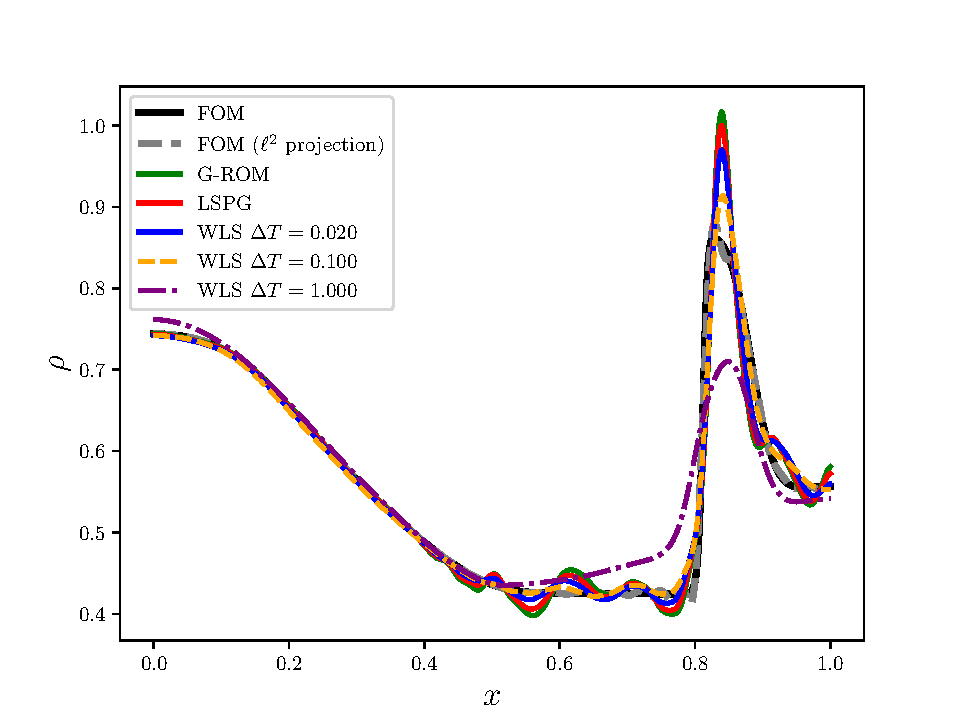
\includegraphics[width=1.\linewidth]{figs/sod/rho_t05_compare.pdf}
\caption{$t=0.5$}
\end{subfigure}
\begin{subfigure}[t]{0.45\textwidth}
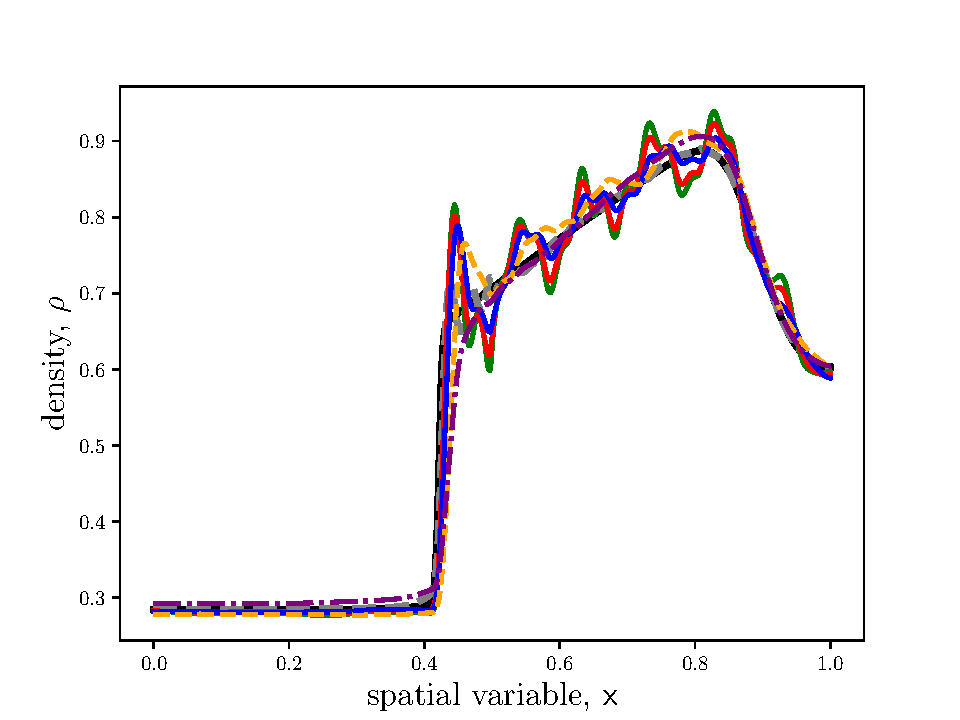
\includegraphics[width=1.\linewidth]{figs/sod/rho_t1_compare.pdf}
\caption{$t=1$}
\end{subfigure}
\caption{Density profiles at various time instances.}
\label{fig:sod_density}
\end{center}
\end{figure}


\begin{figure}
\begin{center}
\begin{subfigure}[t]{0.48\textwidth}
\includegraphics[width=1.\linewidth]{figs/sod/xt_fom.pdf}
\caption{Full-order model}
\end{subfigure}
\begin{subfigure}[t]{0.48\textwidth}
\includegraphics[width=1.\linewidth]{figs/sod/xt_grom.pdf}
\caption{G-ROM}
\end{subfigure}
\begin{subfigure}[t]{0.48\textwidth}
\includegraphics[width=1.\linewidth]{figs/sod/xt_lspg.pdf}
\caption{LSPG}
\end{subfigure}
\begin{subfigure}[t]{0.48\textwidth}
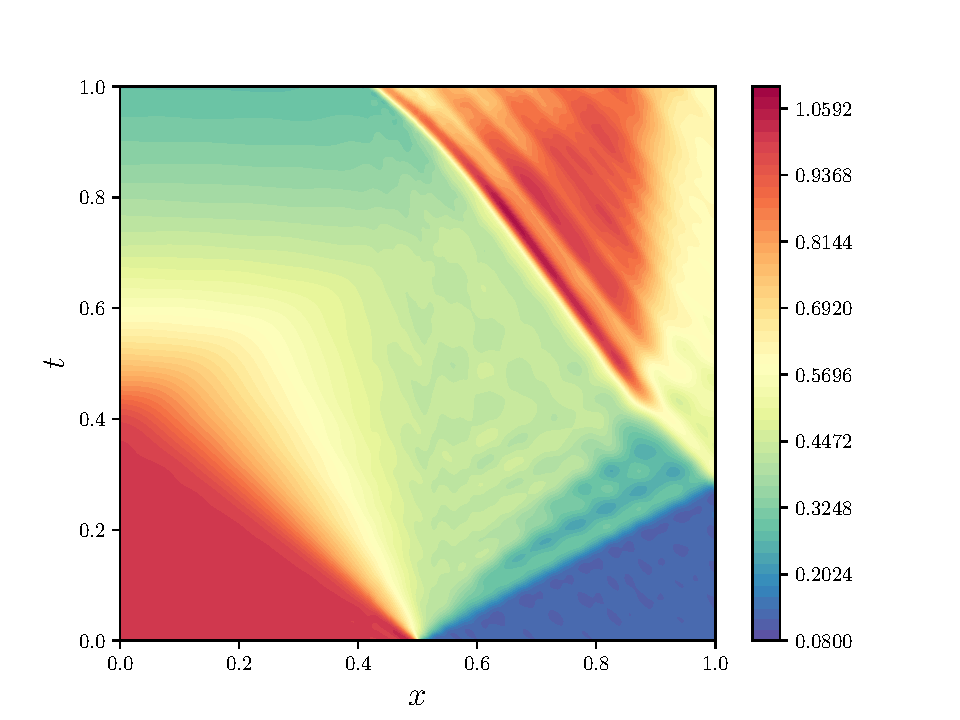
\includegraphics[width=1.\linewidth]{figs/sod/xt_w1.pdf}
\caption{\methodAcronym: $\DeltaSlabArg{}= 0.002$}
\end{subfigure}
\begin{subfigure}[t]{0.48\textwidth}
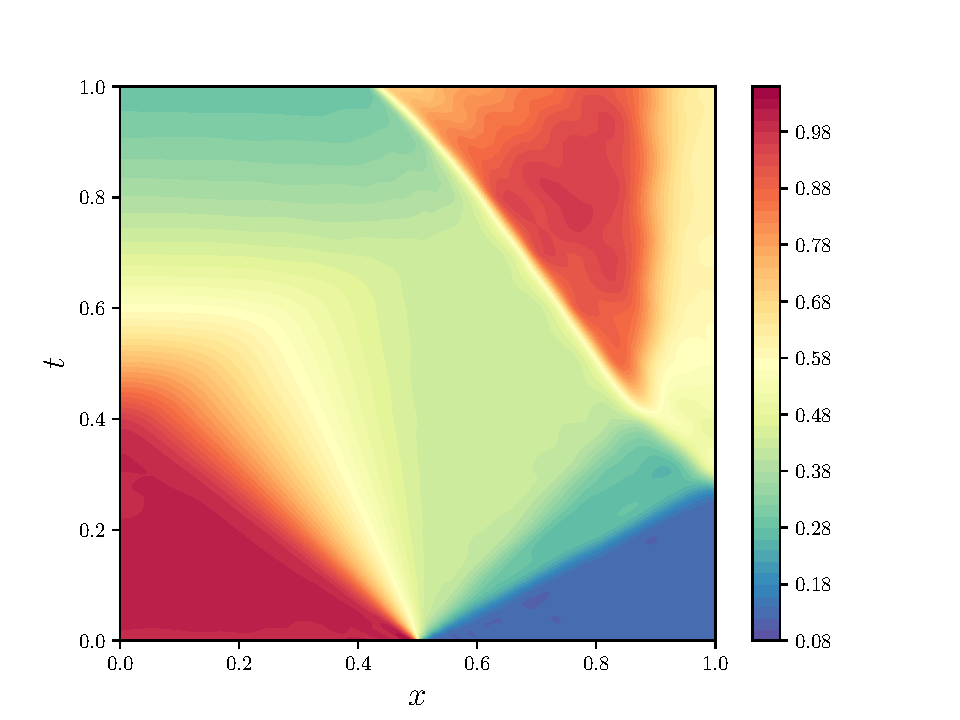
\includegraphics[width=1.\linewidth]{figs/sod/xt_w50.pdf}
\caption{\methodAcronym: $\DeltaSlabArg{} = 0.1$}
\end{subfigure}
\begin{subfigure}[t]{0.48\textwidth}
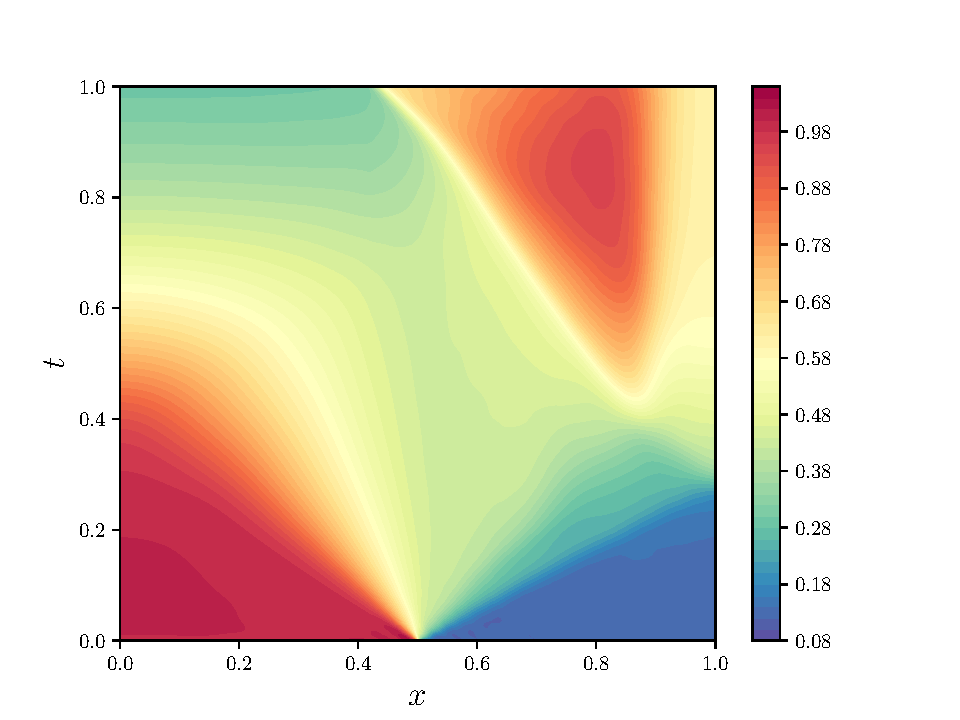
\includegraphics[width=1.\linewidth]{figs/sod/xt_w500.pdf}
\caption{\methodAcronym: $\DeltaSlabArg{} = 1.0$}
\end{subfigure}
\caption{$\mathsf{x}-t$ diagrams for the density fields as predicted by the FOM, G-ROM,
	LSPG-ROM, and \methodAcronymROMs.}
\label{fig:sod_xt}
\end{center}
\end{figure}

Next, Figure~\ref{fig:sod_error} shows time-integrated $\ell^2$-norm of the state errors and the objective function~\eqref{eq:obj} (i.e., the time-integrated residual norm) over $t \in [0,1]$ for the various ROMs. Most notably, we observe 
that increasing the window size over which the residual is minimized does \textit{not} lead to a monotonic decrease in the error as measured in the time-integrated $\elltwo$-norm (we refer to this as the $\elltwo$-error). As expected, increasing the window size does lead to a monotonic decrease in the time-integrated residual norm, however. We additionally note that, although the time-integrated $\elltwo$-error of 
the projected FOM solution is significantly lower than that of the various ROM solutions, the time-integrated residual norm of the projected FOM solution is \textit{higher} 
than all ROMs. Thus, although the projected FOM solution is more accurate in the $\elltwo$-norm, it does not satisfy the governing equations as well the ROM solutions. 

\begin{figure}
\begin{center}
\begin{subfigure}[t]{0.45\textwidth}
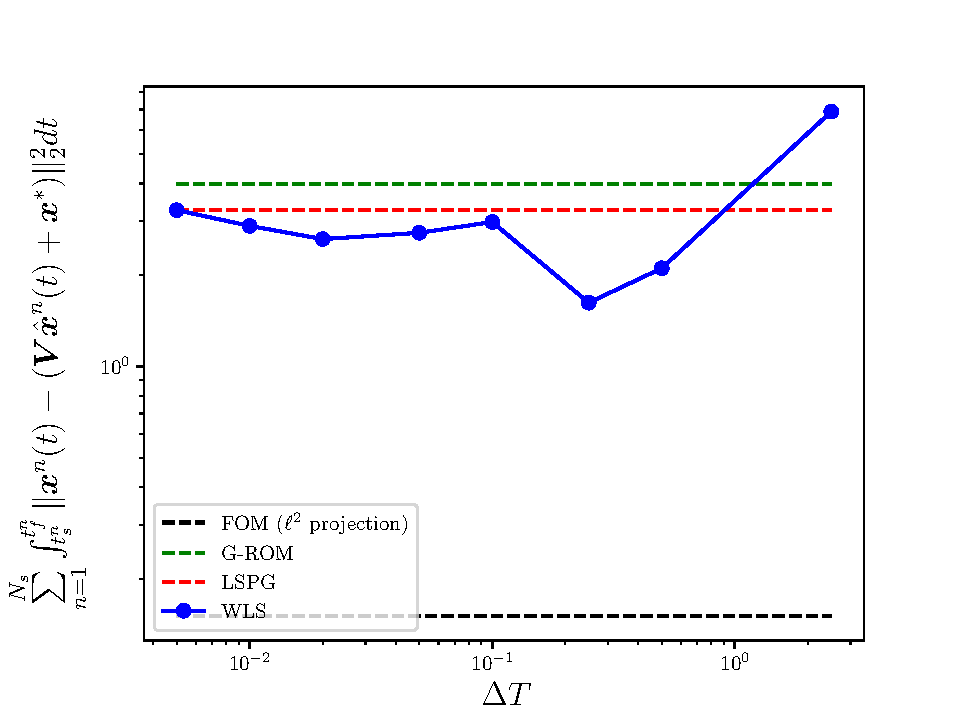
\includegraphics[width=1.\linewidth]{figs/sod/error_vs_window_compare.pdf}
\caption{Relative time-integrated $\elltwo$-error of various ROMs.}
\label{fig:sod_error_a}
\end{subfigure}
\begin{subfigure}[t]{0.45\textwidth}
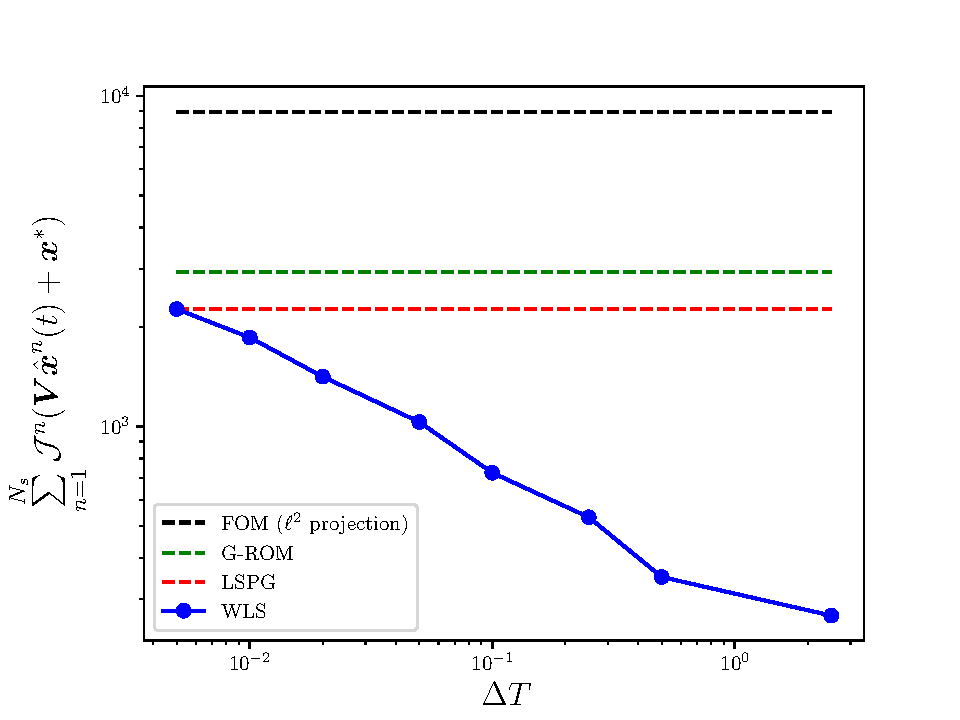
\includegraphics[width=1.\linewidth]{figs/sod/objective_vs_window_compare.pdf}
\caption{Time-integrated residual norm of various ROMs.} 
\label{fig:sod_error_b}
\end{subfigure}
\caption{Time-integrated performance metrics of the Galerkin, LSPG, and \methodAcronymROMs.  Note that the Galerkin and LSPG ROMs do not depend on the window size.} 
\label{fig:sod_error}
\end{center}
\end{figure}

We now examine the comparative performance of the direct and indirect solution techniques for the \methodAcronymROMs\ using various time discretization techniques. 
Figure~\ref{fig:sod_error_methods} 
shows the same time-integrated $\elltwo$-errors and residual norms as in Figure~\ref{fig:sod_error}, but this time results are shown for 
the various \methodAcronymROMs. In both Figures~\ref{fig:sod_error_methods_a} and~\ref{fig:sod_error_methods_b}, we observe that the \methodAcronym\ method 
is relatively insensitive to the solution technique (direct vs indirect) and underlying discretization scheme, although some minor differences are observed.
In particular, ROMs using the second order explicit AB2 scheme with a time step of $\Delta t = 0.0005$ provide similar results to the 
ROMs using the second-order CN scheme at a time step of $\Delta t = 0.002$. All methods display similar dependence on the window size: the optimal time-integrated 
$\elltwo$-error occurs when the window size is $\DeltaSlabArg{} = 0.1$, and the time-integrated residual norm decreases monotonically as the window size grows. 
\begin{figure}
\begin{center}
\begin{subfigure}[t]{0.45\textwidth}
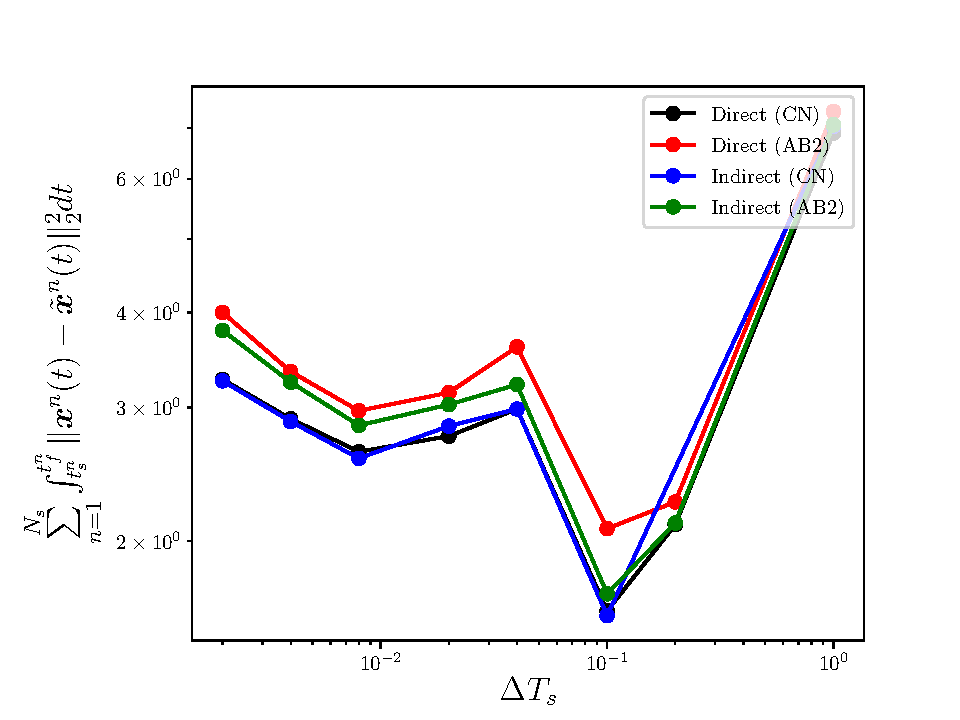
\includegraphics[width=1.\linewidth]{figs/sod/error_vs_window.pdf}
\caption{Relative time-integrated $\elltwo$-error of the \methodAcronymROMs.}
\label{fig:sod_error_methods_a}
\end{subfigure}
\begin{subfigure}[t]{0.45\textwidth}
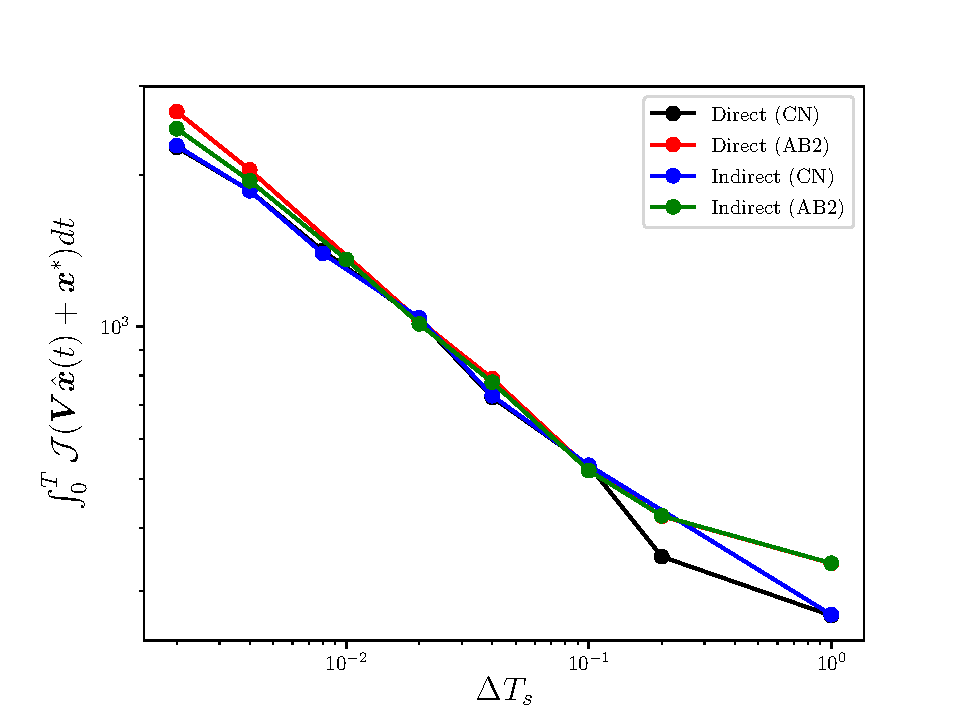
\includegraphics[width=1.\linewidth]{figs/sod/objective_vs_window.pdf}
\caption{Time-integrated residual norm of the \methodAcronymROMs.} 
\label{fig:sod_error_methods_b}
\end{subfigure}
\caption{Time-integrated performance metrics of various \methodAcronymROMs.} 
\label{fig:sod_error_methods}
\end{center}
\end{figure}


Next, Figure~\ref{fig:sod_walltime} provides the CPU wall-clock times for the various \methodAcronymROMs. We observe that the computational cost of all methods grows
as the window size is increased. For indirect methods, this increase in cost is due to the fact that, as the window size 
grows, more iterations of the FBSM are required for convergence. For direct methods, the increase in cost is due to (1) the cost 
associated with forming and solving the normal equations at each Gauss--Newton iteration and (2) the increased number of 
Gauss--Newton iterations required for convergence. We observe the cost of the FBSM method to increase more rapidly 
than the direct methods. Encouragingly, \methodAcronymROMs\ based on the CN discretization
minimizing the full space--time residual (comprising 
500 time instances) only  
cost approximately one order of magnitude more than the case where the residual is minimized over a single time step (i.e., LSPG). Also of interest is the 
fact that the direct method utilizing the AB2 time-discretization scheme costs only slightly more per a given window size than the direct method 
utilizing the CN time discretization. This is despite the fact that AB2 is evolved at a time step of $\Delta t = 0.0005$, while CN uses $\Delta t = 0.002$; thus 
AB2 contains 4 times more temporal degrees of freedom than CN.  Finally, we emphasize that the 
results presented here are for standard algorithms (e.g., Gauss--Newton and the FBSM). As mentioned in 
Remarks~\ref{remark:gaussnewton} and~\ref{remark:fbsm}, we expect that the computational cost 
of both indirect and direct methods can be decreased through the use and/or development of 
algorithms tailored to the windowed minimization problem. 


\begin{figure}
\begin{center}
\begin{subfigure}[t]{0.45\textwidth}
%\includegraphics[width=1.\linewidth]{/Users/ejparis/PyROM/pyrom/sod/postProcess_wv/error_vs_window.pdf}
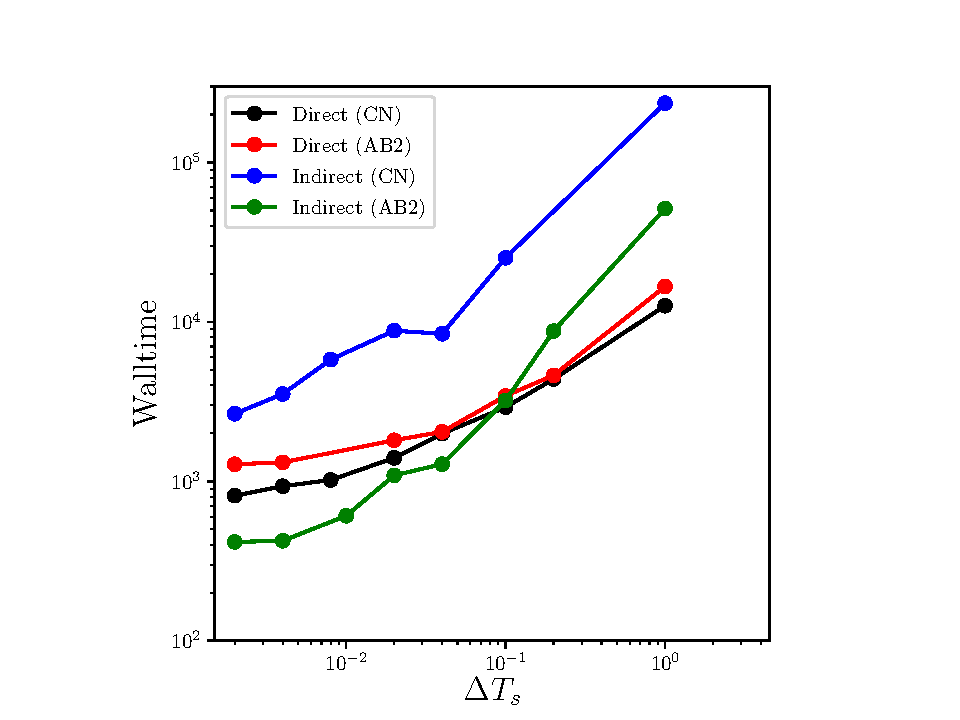
\includegraphics[width=1.\linewidth]{figs/sod/walltime_vs_window.pdf}
\label{fig:sod_error_a}
\end{subfigure}
\caption{Comparison of wall-clock times of the direct and indirect \methodAcronymROMs\ as a function of window size.} 
\label{fig:sod_walltime}
\end{center}
\end{figure}

Next, we study the impact of the time step on the \methodAcronymROM\ results. We examine \methodAcronymROMs\ that use a
window size of $\Delta T = 0.1$, with time steps $\Delta t =$  $0.001$, $0.002$, $0.005$, $0.01$, $0.05$, $0.1$ (i.e.,  
$100$, $50$, $20$, $10$, $2$, and $1$ time instances per window). We additionally 
consider LSPG ROMs leveraging the same set of time steps. To assess time step convergence, we compare results to a new full-order model, which is as described in Section~\ref{sec:sod_fom} but uses a fine time step of $\Delta t = 10^{-4}$. Figure~\ref{fig:time_step_study} shows the time-integrated $\elltwo$-error and residual norm  
of the various ROMs. We observe that the time-integrated $\elltwo$-error and residual norm 
of the \methodAcronymROMs\ decrease and converge as the time step decreases. This is in direct contrast to the LSPG ROMs, in where the time-integrated $\elltwo$-error and residual norm display a complex dependence on the time step. This result 
demonstrates that \methodAcronym\ overcomes the time-step dependence inherit to the LSPG approach. Lastly, Figure~\ref{fig:walltime_dtvar}
shows the relative wall-clock times of the \methodAcronymROMs\ with respect to the LSPG ROMs. It is seen that for all time steps considered, the \methodAcronymROMs\ 
are less than 6x the cost of LSPG; this is despite the window sizes comprising up to 100 time instances. 
\begin{figure}
\begin{center}
\begin{subfigure}[t]{0.45\textwidth}
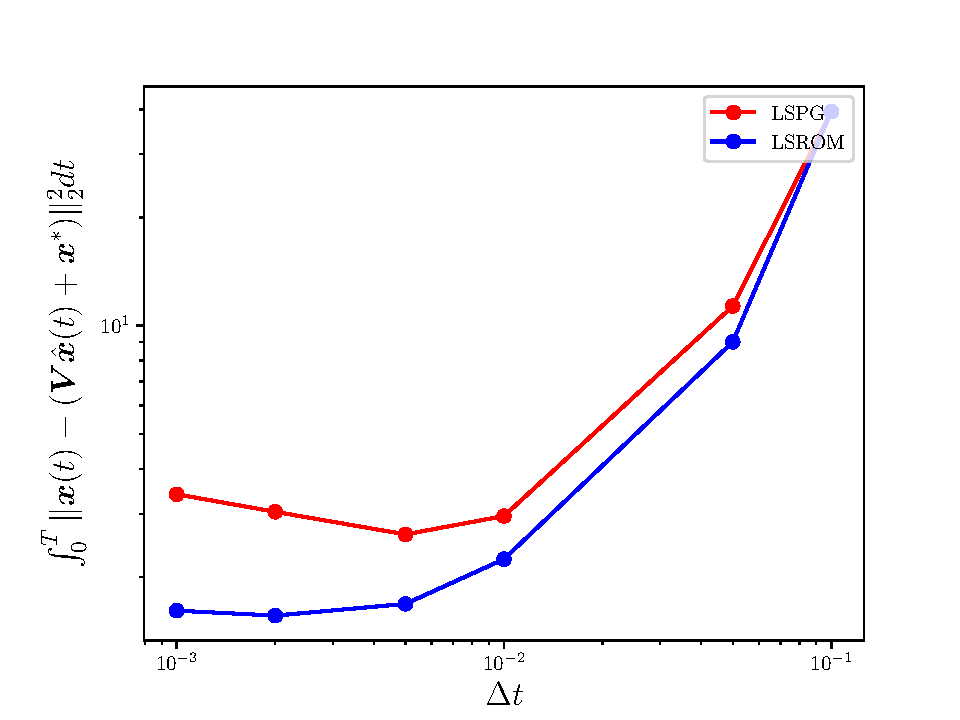
\includegraphics[width=1.\linewidth]{figs/sod/error_vs_window_dtvar.pdf}
\caption{Relative time-integrated $\elltwo$-error of the \methodAcronymROM.}
\label{fig:sod_error_methods_a}
\end{subfigure}
\begin{subfigure}[t]{0.45\textwidth}
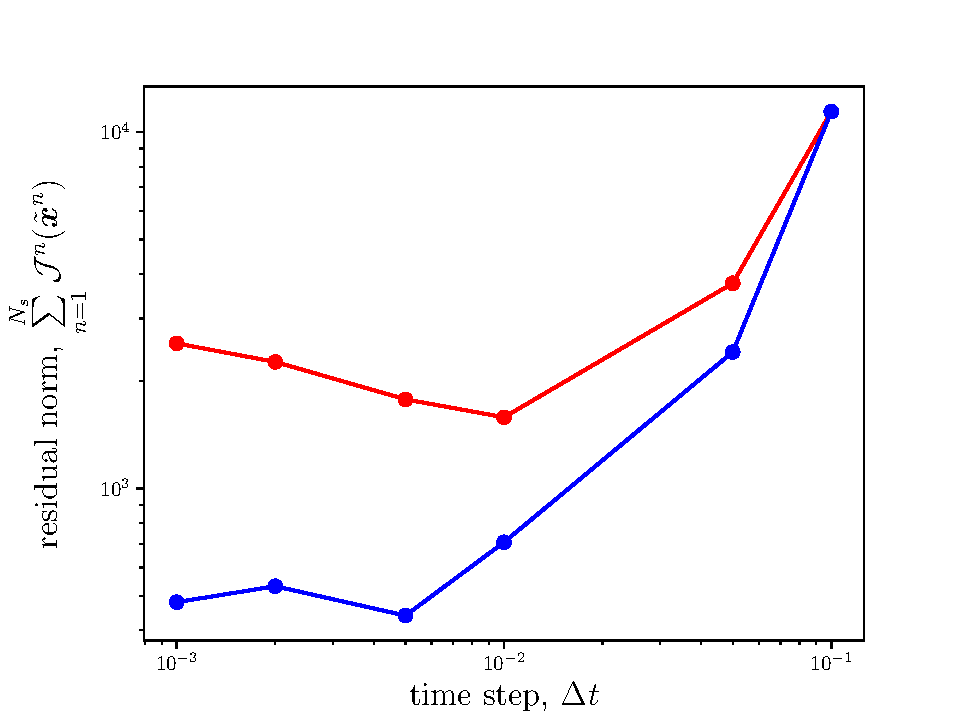
\includegraphics[width=1.\linewidth]{figs/sod/objective_vs_window_dtvar.pdf}
\caption{Time-integrated residual norm of the \methodAcronymROM.} 
\label{fig:sod_error_methods_b}
\end{subfigure}
\caption{Performance metrics of the Galerkin, LSPG, and \methodAcronymROMs.} 
\label{fig:time_step_study}
\end{center}
\end{figure}

\begin{figure}
\begin{center}
\begin{subfigure}[t]{0.45\textwidth}
%\includegraphics[width=1.\linewidth]{/Users/ejparis/PyROM/pyrom/sod/postProcess_wv/error_vs_window.pdf}
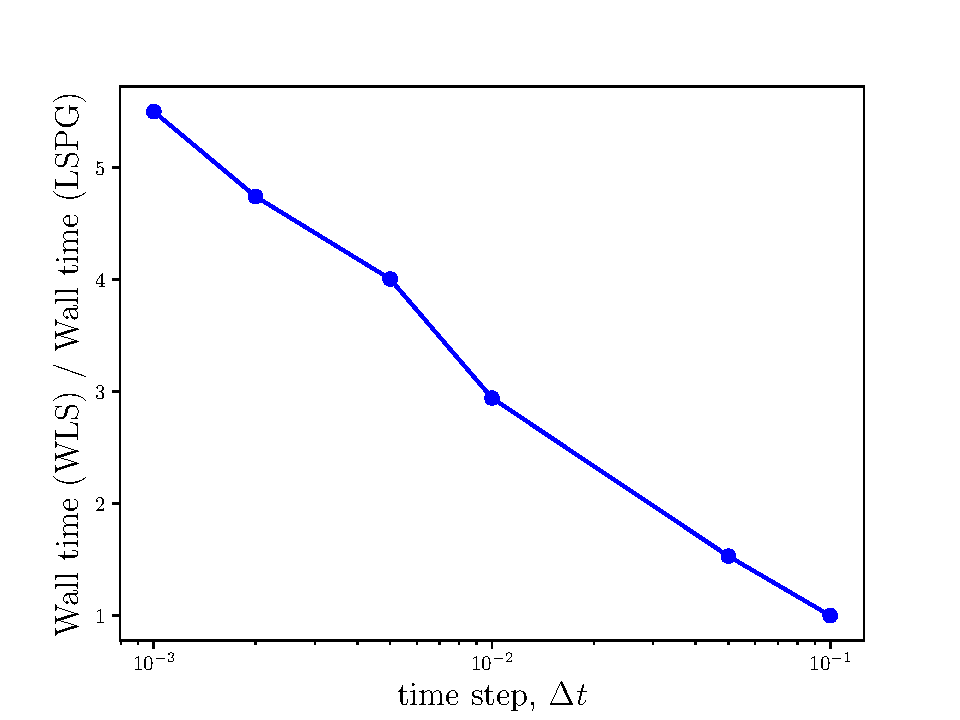
\includegraphics[width=1.\linewidth]{figs/sod/walltime_vs_window_dtvar.pdf}
\label{fig:sod_error_a}
\end{subfigure}
\caption{Comparison of wall-clock times of the \methodAcronymROMs\ to LSPG ROMs as a function of the time step. WLS ROMs have a fixed window size of $\Delta T = 0.1$.} 
\label{fig:walltime_dtvar}
\end{center}
\end{figure}


\subsubsection{Results as a function of basis dimension}
Lastly, we assess the impact of the basis dimension on the performance of the various reduced-order models. We again consider S-reduction trial subspaces. We obtain the trial subspaces by evolving the FOM for $t \in [0.0,1.0]$ at a time-step of $\Delta t = 0.002$ with the CN scheme. We execute Algorithm~\ref{alg:pod} with inputs $N_{\text{skip}} = 2$, $\stateIntercept = \state_0$\footnote{We observed negative pressures in the projected initial conditions for trial subspaces of dimension $K=20,30,40$ if we used the offset $\stateIntercept = \bz$. Thus, for our convergence study we employed $\stateIntercept = \state_0$ so-as to avoid negative pressures in the projected initial conditions.}, and $\romdim = 10,20,30,40,50$. We investigate reduced-order models based on Galerkin projection, LSPG projection, and the WLS approach. All methods leverage the CN time scheme with $\Delta t = 0.002$. We present results for windows of size $\Delta T^n \equiv \Delta T = 0.002,0.004,0.02,0.04,0.10$ for the WLS approach. All WLS ROMs are solved via the direct approach described previously. 

Figure~\ref{fig:convergence_study} shows the time-integrated $\ell^2$-error of the various ROM solutions, as well as that of the optimal solution as measured in the $\ell^2$-norm (i.e., the orthogonal projection of the FOM solution onto the trial subspace). In Figure~\ref{fig:sod_error_converge} we first observe that for a basis of dimension $\romdim = 10$, the Galerkin, LSPG, and WLS ($\Delta T = 0.002$, $\Delta T = 0.004$) ROMs do not converge. Upon investigation, this lack of convergence occurred due to the presence of negative pressure. We next observe that the time-integrated $\ell^2$-error monotonically decreases as the basis dimension increases for all remaining ROM solutions with the exception of the Galerkin, LSPG, and WLS ($\Delta T = 0.002$, $\Delta T = 0.004$) ROMs at the dimension $\romdim = 30$. Overall, we observe that larger window sizes yield lower errors when the basis dimension is small. For larger basis dimensions we observe all ROMs to yield accurate solutions, and a larger window size does not always yield a lower error. In Figure~\ref{fig:sod_residual_converge}, we next observe that the time-integrated residual norm monotonically decreases as the basis dimension grows. This result is supported, although not guaranteed, by the error analysis presented in Section~\ref{sec:analysis} (and Ref.~\cite{carlberg_lspg_v_galerkin} for LSPG). Finally, we observe that larger window sizes yield lower time-integrated residuals.  

\begin{figure}
\begin{center}
\begin{subfigure}[t]{0.45\textwidth}
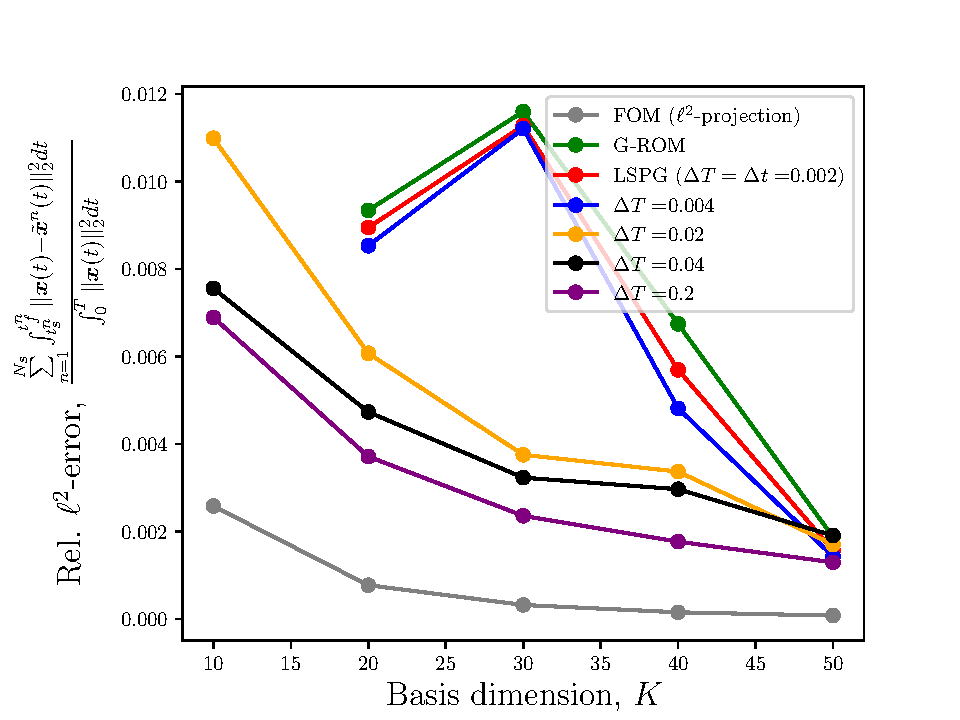
\includegraphics[width=1.\linewidth]{figs/sod/error_converge.pdf}
\caption{Relative time-integrated $\elltwo$-error of the \methodAcronymROM.}
\label{fig:sod_error_converge}
\end{subfigure}
\begin{subfigure}[t]{0.45\textwidth}
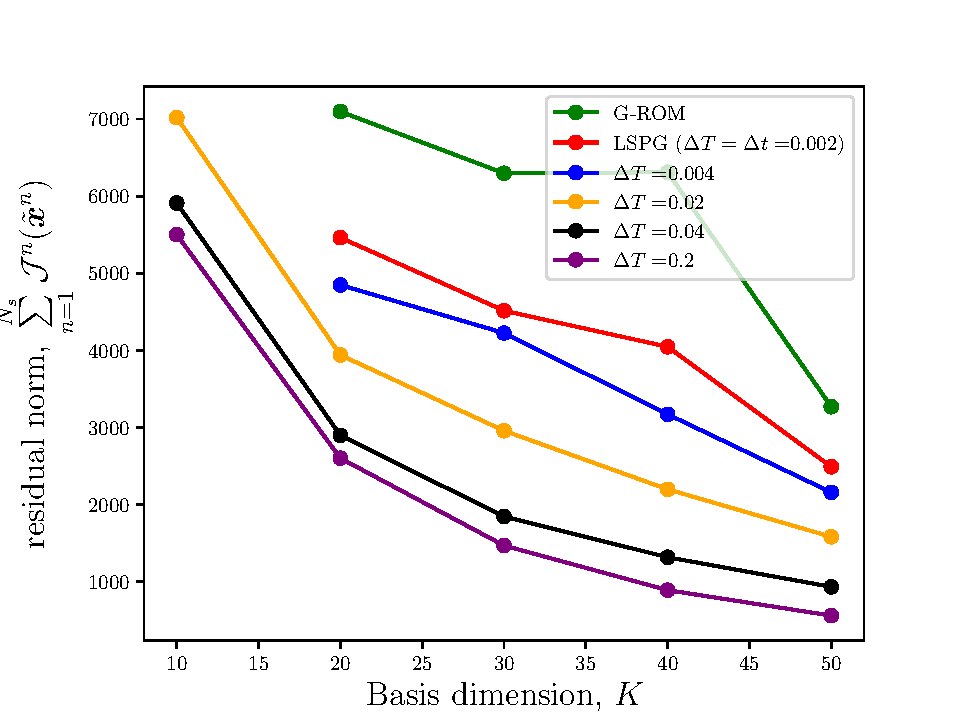
\includegraphics[width=1.\linewidth]{figs/sod/residual_converge.pdf}
\caption{Time-integrated residual norm of the \methodAcronymROM.} 
\label{fig:sod_residual_converge}
\end{subfigure}
\caption{Performance metrics of the Galerkin, LSPG, and \methodAcronymROMs\ as a function of basis dimension. Missing entries indicate that the solver did not converge.} 
\label{fig:convergence_study}
\end{center}
\end{figure}

Next, Figure~\ref{fig:convergence_study_pareto} presents Pareto plots for the time-integrated $\elltwo$-error and residual as a function of wall-clock time for ROMs with varying basis dimensions and window sizes. We observe intermediate window sizes (i.e., $\Delta T = 0.02,0.04$) to be Pareto-optimal for the error (i.e., lowest CPU time for a given error tolerance) for all runs with the exception of the $K=50$ case, in which case window sizes of $\Delta T = 0.002$ (i.e., LSPG) and $\Delta T = 0.004$ are Pareto-optimal. We next observe that intermediate window sizes are Pareto-optimal for the integrated residual norm for all cases, with the exception of runs using $\Delta T = 0.02, 0.04$, and $K=20$. Summing across the Pareto plots for the time-integrated error and residual, we find that --- for the window sizes and bases considered --- $\Delta T = 0.002$ (i.e., LSPG) is Pareto optimal three times, $\Delta T = 0.004$ one time, $\Delta T = 0.02$ 2 times, $\Delta T = 0.04$ 6 times, and $\Delta T = 0.2$ two times.  


\begin{figure}
\begin{center}
\begin{subfigure}[t]{0.45\textwidth}
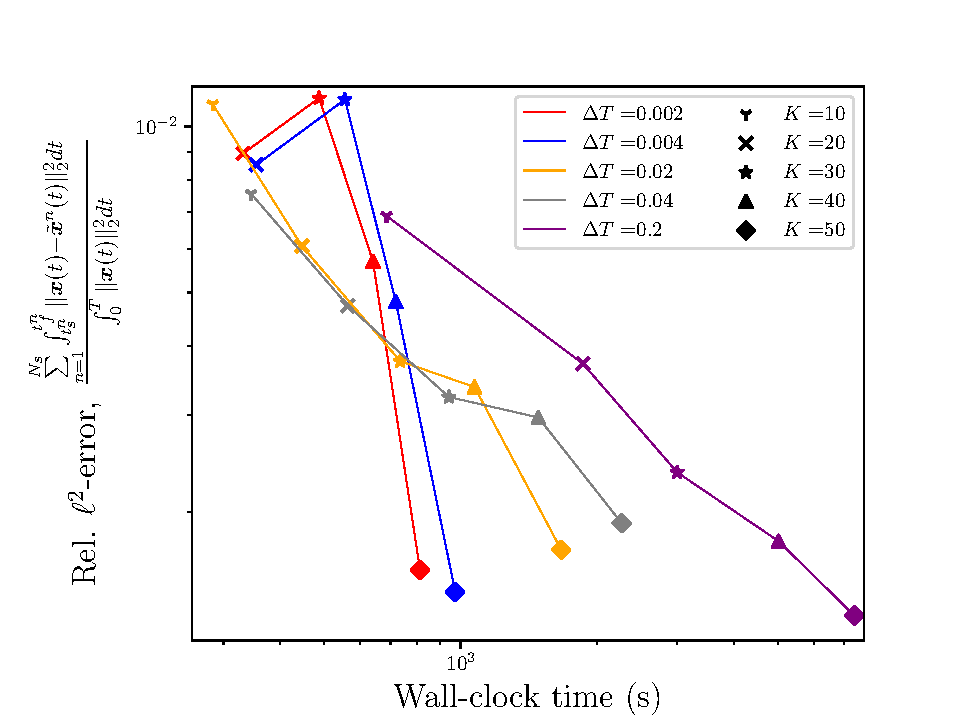
\includegraphics[width=1.\linewidth]{figs/sod/pareto_error.pdf}
\caption{Relative time-integrated $\elltwo$-error of the \methodAcronymROM.}
\label{fig:sod_error_converge}
\end{subfigure}
\begin{subfigure}[t]{0.45\textwidth}
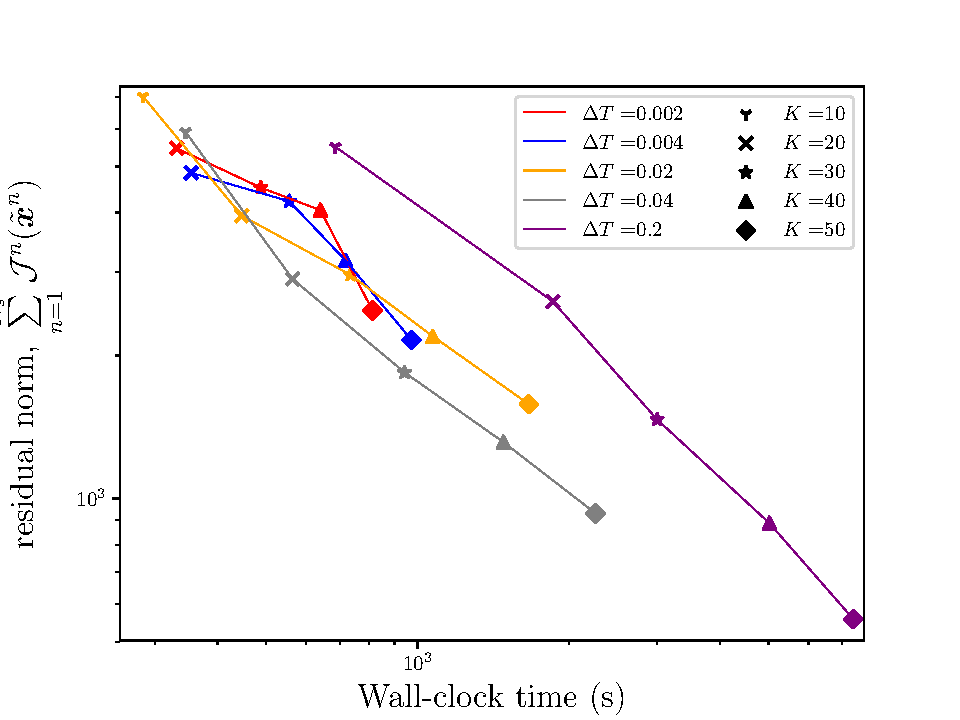
\includegraphics[width=1.\linewidth]{figs/sod/pareto_resids.pdf}
\caption{Time-integrated residual norm of the \methodAcronymROM.} 
\label{fig:sod_residual_converge}
\end{subfigure}
\caption{Pareto fronts for the time-integrate $\elltwo$-error (left) and time-integrated residual norm (right) as a function of wall-clock time.} 
\label{fig:convergence_study_pareto}
\end{center}
\end{figure}

\begin{figure}
\begin{center}
\begin{subfigure}[t]{0.45\textwidth}
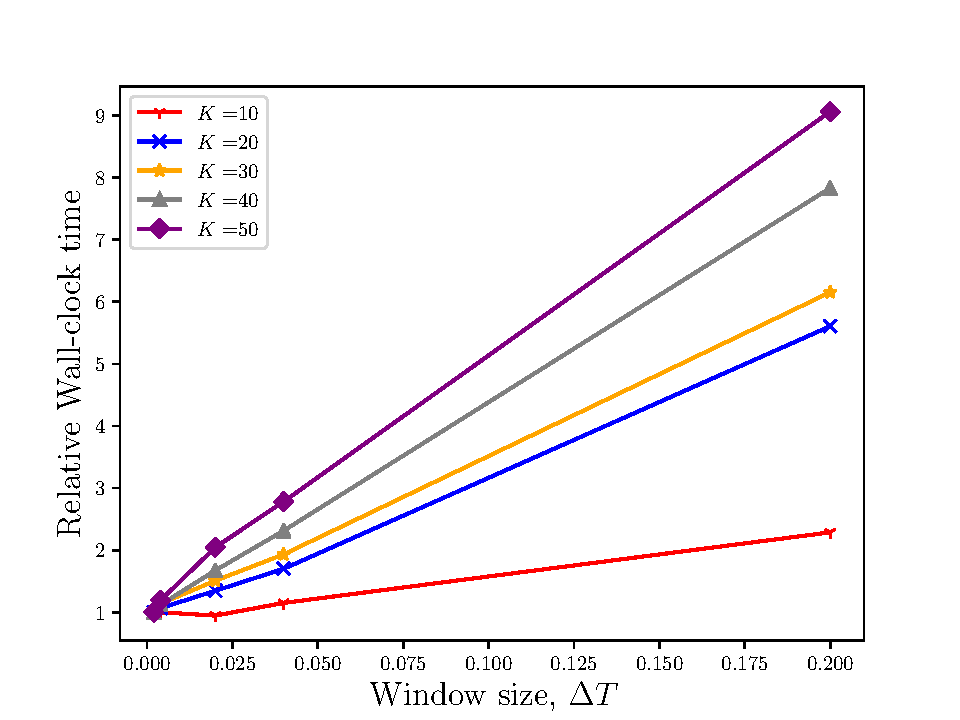
\includegraphics[width=1.\linewidth]{figs/sod/converge_walltimes.pdf}
\caption{Relative time-integrated $\elltwo$-error of the \methodAcronymROM.}
\label{fig:sod_error_converge}
\end{subfigure}
\caption{Performance metrics of the Galerkin, LSPG, and \methodAcronymROMs\ as a function of basis dimension. Missing entries indicate that the solver did not converge.} 
\label{fig:convergence_study}
\end{center}
\end{figure}


\subsubsection{Summary of numerical results for the Sod shock tube}
The key observations from the results of the first numerical example are: 
\begin{enumerate}
\item Increasing the window size over which the residual is minimized led to more physically relevant solutions. Specifically, we observed that as the window size over which the residual was minimized grew, \methodAcronym\ led to less oscillatory solutions.
\item Increasing the window size over which the residual is minimized does not necessary lead to a lower space--time error as measured by the $\elltwo$-norm. We observed that minimizing the residual over an intermediary window size led to the lowest space--time error in the $\elltwo$-norm. 
\item \methodAcronym\ displays time-step convergence: both the $\elltwo$-error and residual norm decreased and displayed time-step convergence as the time step decreased. This is in contrast to LSPG.
\item For all examples considered, in where the windows comprised up to 2000 time instances, \methodAcronym\ with the direct method is between 1x and 10x the cost of the LSPG. The 
direct method was observed to be slightly more efficient and robust than the indirect method.
\end{enumerate} 

\subsection{Cavity Flow}
The next numerical example considers hyper-reduced ROMs of a viscous, compressible flow in a two-dimensional cavity. 
The flow is described by the two-dimensional compressible Navier-Stokes equations,
\begin{equation}\label{eq:compressible_ns}
\frac{\partial \mathbf{u}}{\partial t} + \nabla \cdot \big( \mathbf{F}(\mathbf{u} ) - \mathbf{F}_v (\mathbf{u},\nabla \mathbf{u} )      \big) =\bz,
\end{equation}
where $\mathbf{u}: [0,T] \times \Omega \rightarrow \RR{4}$ comprise the density, x and y momentum, and total energy. The terms $\mathbf{F}$ and $ \mathbf{F}_v$ are the inviscid and viscous fluxes, respectively. For a two-dimensional flow, the state vector and inviscid fluxes are
$$
\mathbf{u} = \begin{Bmatrix}
\rho \\ \rho u_1 \\ \rho u_2 \\ \rho E \end{Bmatrix}, \qquad \mathbf{F}_{1} = \begin{Bmatrix} \rho u_1 \\ \rho u_1^2 +      p \\ \rho u_1 u_2 \\ u_1(E + p) \end{Bmatrix}, 
\qquad \mathbf{F}_{2} = \begin{Bmatrix} \rho u_2 \\ \rho u_1 u_2  \\ \rho u_2^2 + p \\ u_2(E + p) \end{Bmatrix}.
$$
The viscous fluxes are given by
$$
\qquad \mathbf{F}_{v_1} = \begin{Bmatrix} 0 \\ \tau_{11} \\ \tau_{12}  \\ u_j \tau_{j1} + c_p \frac{\mu}{\text{Pr}} \frac{\partial T}{\partial x_1}  \end{Bmatrix}, 
\qquad \mathbf{F}_{v_2} = \begin{Bmatrix} 0 \\ \tau_{21} \\ \tau_{22}  \\ u_j \tau_{j2} + c_p \frac{\mu}{\text{Pr}} \frac{\partial T}{\partial x_2}  \end{Bmatrix}.
$$
We assume a Newtonian fluid, which leads to a viscous stress tensor of the form,
\begin{equation*}
\tau_{ij} = 2\mu S_{ij},
\end{equation*}
where,
\begin{equation*}
 S_{ij} = \frac{1}{2} \big( \frac{\partial u_i}{\partial \mathsf{x}_j} + \frac{\partial u_j}{\partial \mathsf{x}_i} \big) - \frac{1}{3} \frac{\partial      u_k}{\partial \mathsf{x}_i} \delta_{ij}.
\end{equation*}
The Navier-Stokes equations are closed with a constitutive relationship for a calorically perfect gas,
$$p = (\gamma - 1)( \rho E - \frac{1}{2} \rho u_1^2 - \frac{1}{2} \rho u_2^2 \big),$$
where $\gamma = 1.4$ is the heat-capacity ratio.

Figure~\ref{fig:cav_fig} depicts the domain $\Omega$ and flow conditions. Free-stream boundary conditions 
are used at the inlet, outlet, and top wall of the cavity. No-slip boundary conditions are enforced 
on the bottom wall of the cavity. 

\subsubsection{Description of FOM and Generation of Trial Space}
The full-order model comprises a discontinuous-Galerkin discretization. The discretization 
is obtained by partitioning the domain into $100$ elements in the flow direction and $40$ elements 
in the wall-normal direction. The solution is represented to third order over each element using tensor product polynomials of order $p=2$, 
resulting in $36000$ unknowns for each conserved variable. Spatial discretization via the discontinuous Galerkin method yields a dynamical system 
of the form,
$$\frac{d \state}{dt} = \mass_{\text{DG}} \velocity_{\text{DG}} (\state),$$
where $\mass_{\text{DG}} \in \RR{N \times N}$ is the DG mass matrix and $\velocity_{\text{DG}}: \RR{N} \rightarrow \RR{N}$ is the DG velocity operator containing 
surface and volume integrals. By the definition of the FOM~\eqref{eq:FOM}, the dynamical system velocity is $\velocity = \mass_{\text{DG}} \velocity_{\text{DG}}$. 
Figure~\ref{fig:cav_mesh} shows the computational mesh. The 
DG method leverages the Rusanov flux at the cell interfaces~\cite{rusanov} and uses the first form of Bassi and Rebay~\cite{br1} for the viscous fluxes. Time integration 
is performed via a third-order strong stability preserving Runge-Kutta method~\cite{ssp_rk3} with a time-step size of $\Delta t = 0.001$. 
 
The reduced-order models leverage POD to construct the trial basis and use q-sampling~\cite{qdeim_drmac} based on snapshots of the FOM velocity to construct the weighting 
matrix $\stweightingMatArg{n}$. The process used to construct the initial conditions and trial spaces for the ROMs are as follows:
\begin{enumerate}
\item Initialize the FOM with uniform free-stream conditions.
\item Evolve the FOM for $t \in [0,400]$.
\item Reset the time-coordinate, $0 \leftarrow t$, and execute Algorithm~\ref{alg:pod} with $\stateInterceptArg{} = \bz, N_{\text{skip}} = 100$ and $K = \{136,193\}$ over $t \in [0,100]$ to construct two trial spaces comprising $\approx 95\%$ and $\approx 97\%$ of the snapshot energy, respectively. 
\item Execute Algorithm~\ref{alg:qdeim} with $N_{\text{skip}} = 100$, $n_s = 129$ to obtain the sampling point matrix of dimension $\stweightingMatOneArg{} \in \{0,1\}^{1603 \times \fomdim }$. 
\end{enumerate}
Figure~\ref{fig:cav_sampmesh} shows the resulting sample mesh used in the ROM simulations. To depict the nature of the flow, Figure~\ref{fig:fom_sols_cav} shows snapshots of the vorticity field generated by the FOM for several time instances used in training.  
\begin{table}[]
\begin{centering}
\begin{tabular}{c c c c}
\hline
Basis \# & Trial Basis Dimension ($K$) &  Energy Criterion & Sample Points ($n_S$) \\
\hline
%1    & $136$ & $95.0\%$ & $580$ \\
%2    & $193$ & $97.0\%$ & $580$ \\
1    & $136$ & $95.0\%$ & $1603$ \\
2    & $193$ & $97.0\%$ & $1603$ \\
\hline
\end{tabular}
\caption{Summary of the various basis sizes employed in the cavity flow example.}
\label{tab:rom_basis_details}
\end{centering}
\end{table}

\subsubsection{Description of Reduced-Order Models}
Hyper-reduced ROMs based on the Galerkin, collocated Least--Squares Petrov--Galerkin, and \methodAcronym\ approaches are 
again considered. Details on the implementation of the methods is as follows:
\begin{itemize}
\item \textbf{Galerkin ROM with Collocation}: The Galerkin ROM with collocation is obtained through Galerkin projection of the FOM. Unless 
otherwise noted, the  Galerkin ROM is evolved in time with the Crank--Nicolson time scheme at a time step of $\Delta t =0.1$.

\item \textbf{LSPG ROM with Collocation}: The LSPG ROM with collocation is built on top of the FOM discretization using the Crank--Nicolson scheme for temporal 
discretization. Unless otherwise noted, the time step for the LSPG ROM is $\Delta t  = 0.1$. As in the previous example, 
the Gauss--Newton method is used to solve the non-linear least-squares problem arising at each time instance. The Gauss--Newton 
algorithm is deemed converged when the gradient norm is less than $1e-4$. All Jacobians are again computed via automatic differentiation.
 
\item \textbf{\methodAcronymROMs\ with Collocation}: \methodAcronymROMs\ are solved via the direct method. The ROMs use the Crank--Nicolson time-discretization with a time-step size of 
$\Delta t = 0.1$. The Gauss--Newton algorithm is deemed converged when the gradient norm is less than $1e-4$. All Jacobians are computed via automatic differentiation. Uniform quadrature 
weights are used for evaluating the integral in~\eqref{eq:obj_gen_slab}. 
 
%\begin{itemize}
%\item Direct Method: \methodAcronym ROMs solved via the direct method are again implemented with the same Crank--Nicolson time discretization with a nominal 
%time-step size of $\Delta t = 0.1$. 
%\end{itemize}
\end{itemize}


\begin{figure}
\begin{center}
%\begin{subfigure}[t]{0.85\textwidth}
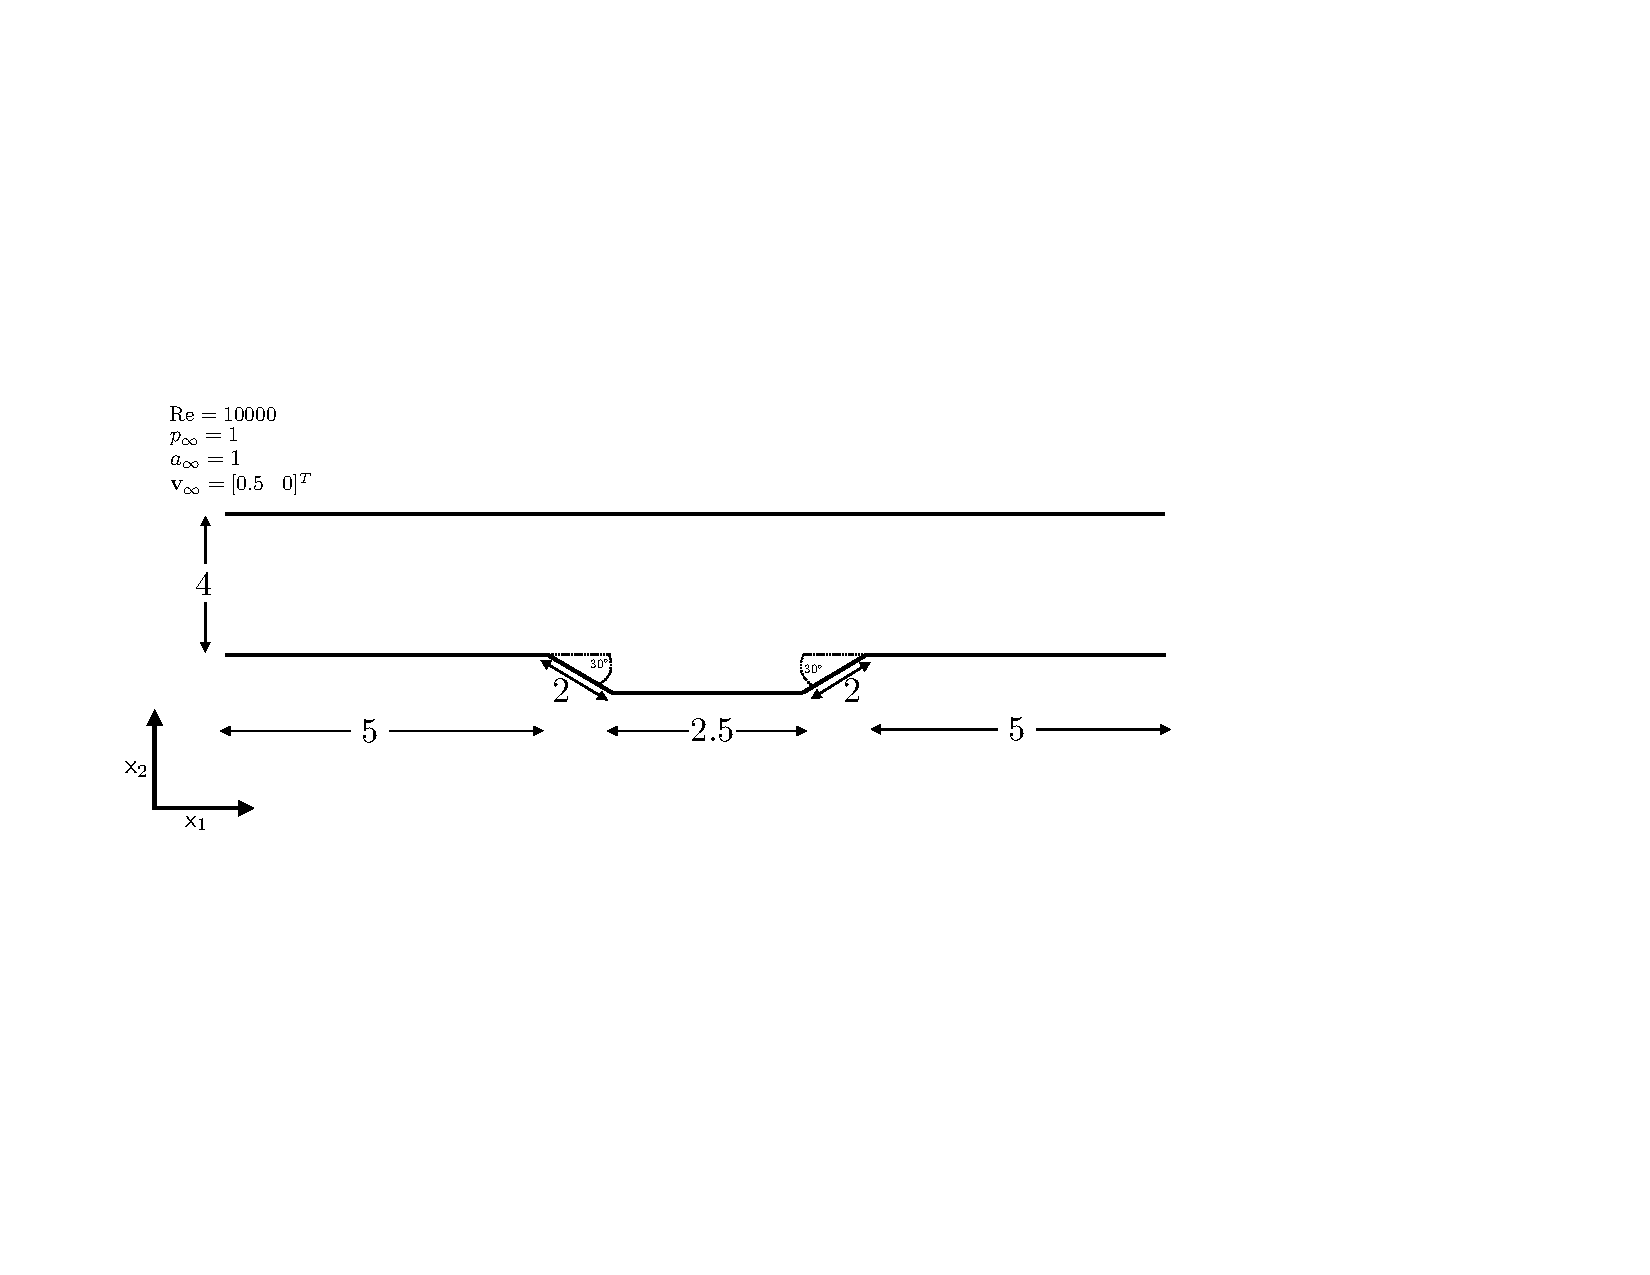
\includegraphics[trim={2cm 7cm 4cm 6cm},clip,width=0.95\linewidth]{cav_fig.pdf}
%\end{subfigure}
\caption{Figure depicting geometry and flow conditions of the cavity flow problem.} 
\label{fig:cav_fig}
\end{center}
\end{figure}

\begin{figure}
\begin{center}
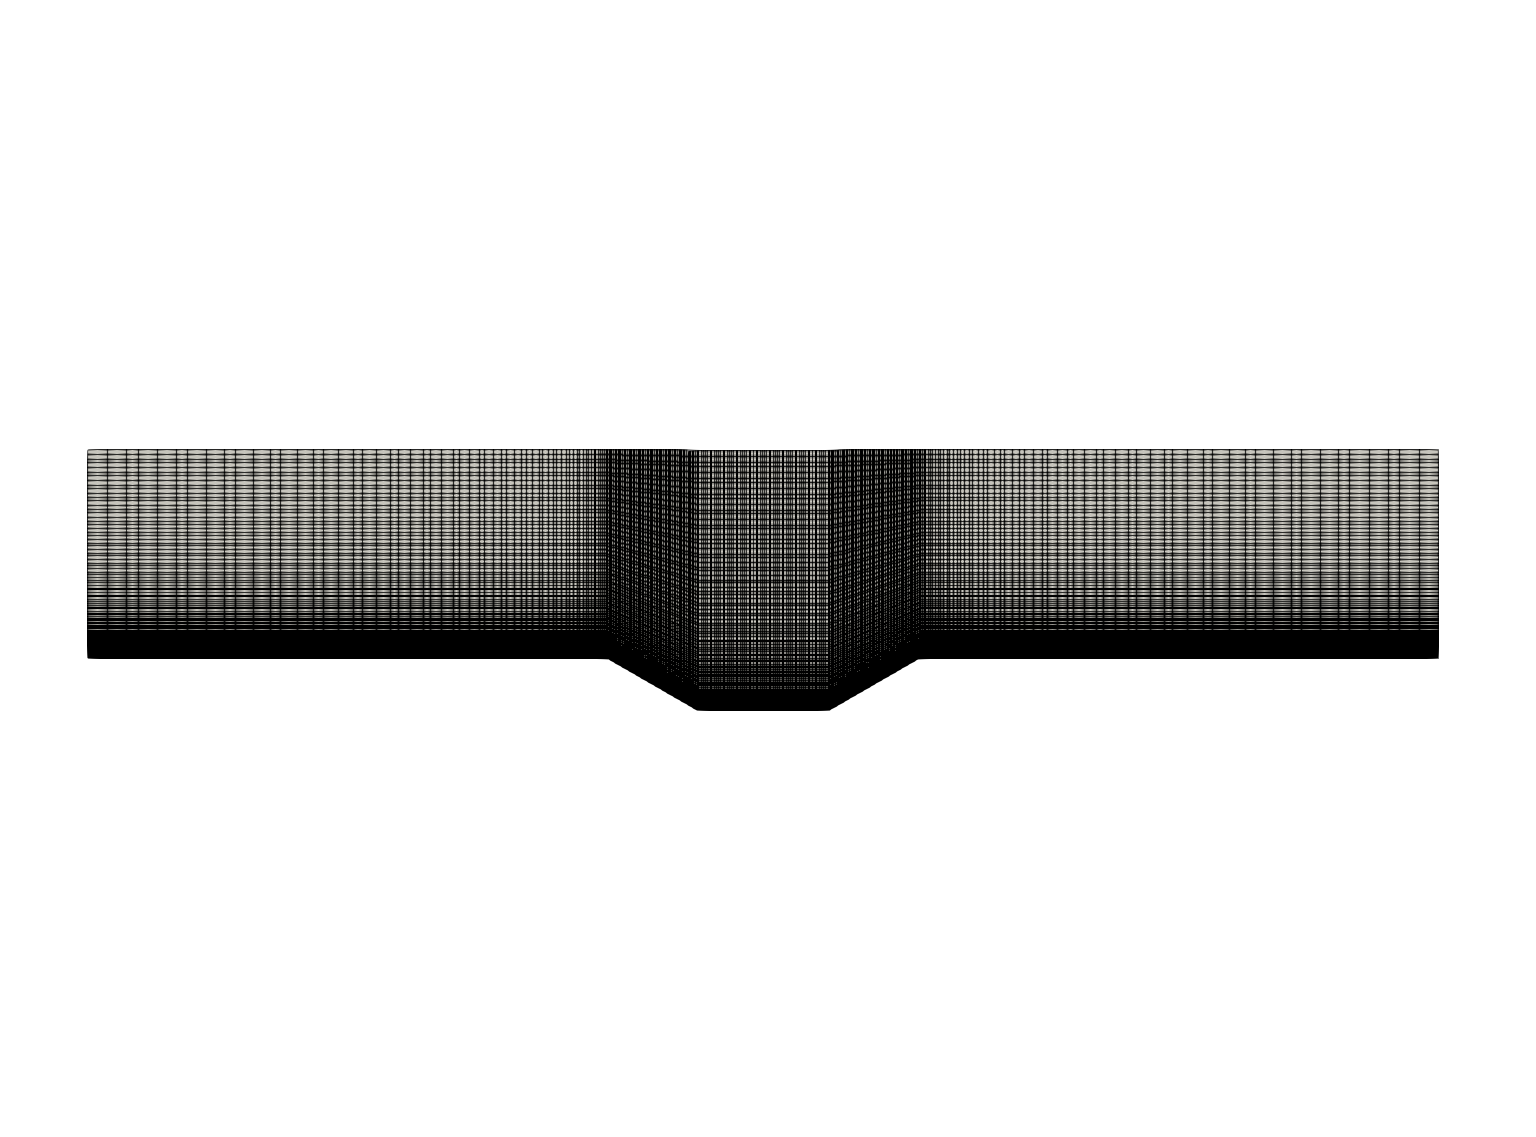
\includegraphics[trim={0cm 14cm 0cm 14cm},clip,width=1.\linewidth]{figs/cavity/grid.png}
\caption{Computational mesh}
\label{fig:cav_mesh}
\end{center}
\end{figure}

\begin{figure} 
\begin{center}
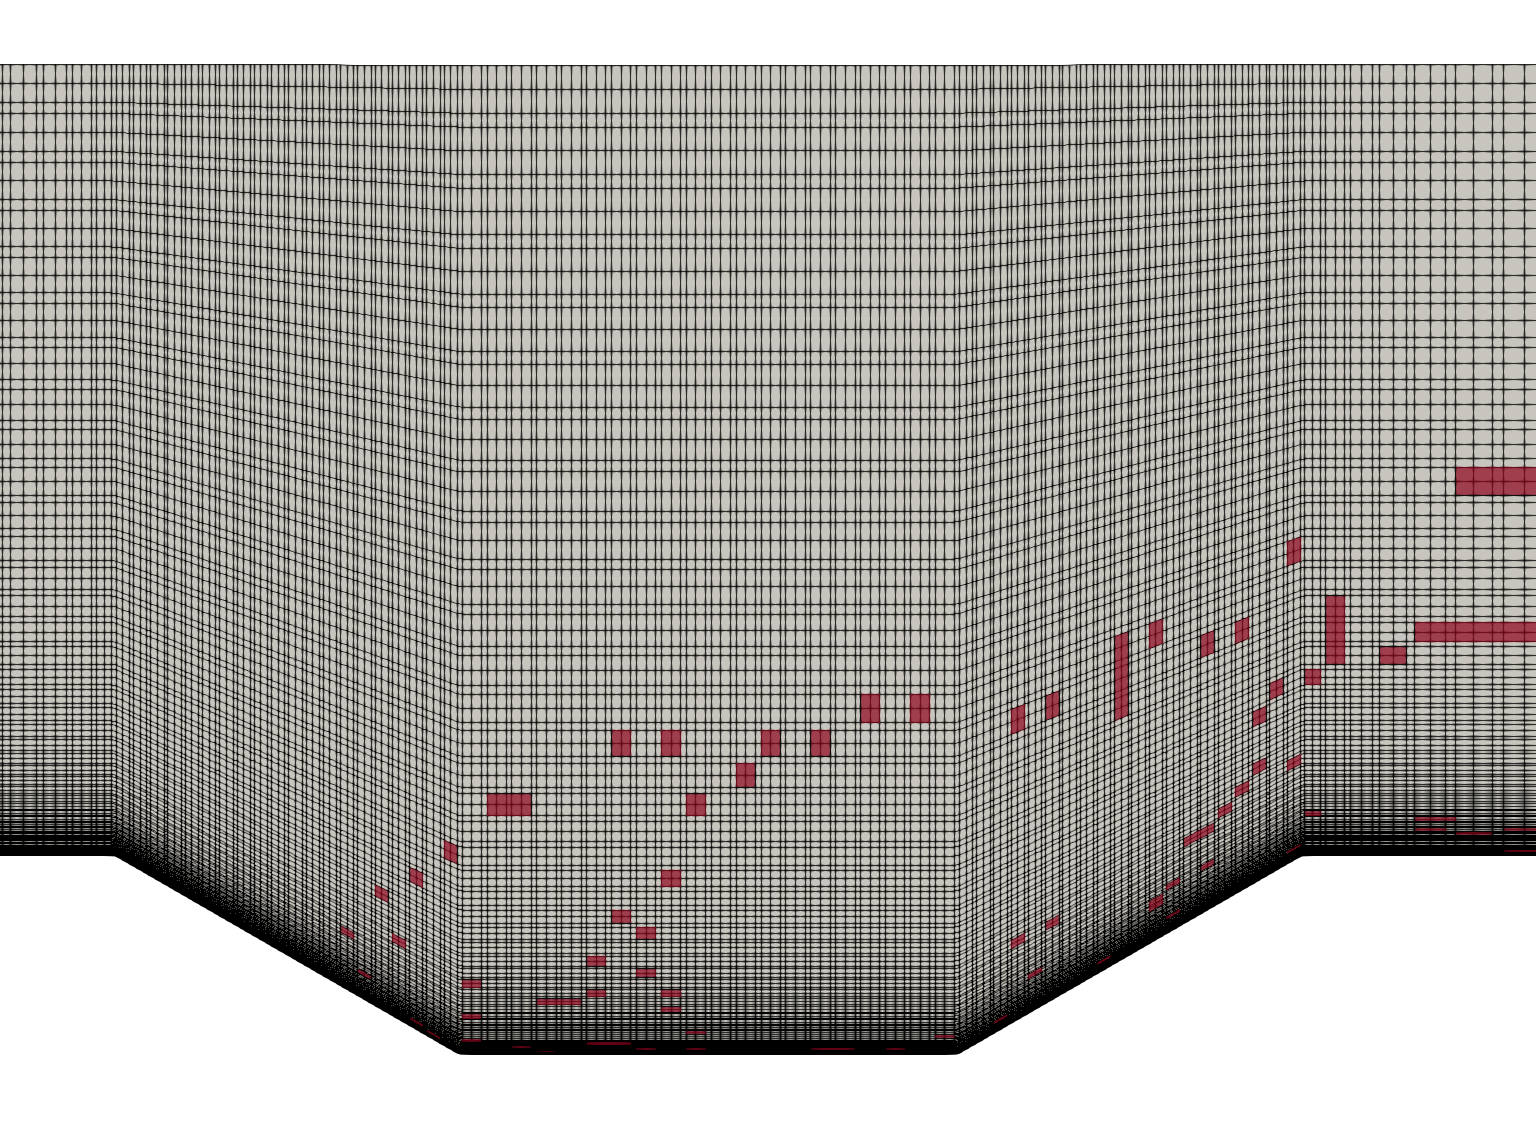
\includegraphics[trim={0cm 0cm 0cm 0cm},clip,width=0.65\linewidth]{figs/cavity/hyper_grid.png}
\caption{Close up of computational mesh with highlighted collocation cells} 
\label{fig:cav_sampmesh}
\end{center}
\end{figure}

\begin{figure}
\begin{center}
%\begin{subfigure}[t]{0.85\textwidth}
\begin{subfigure}[t]{0.49\textwidth}
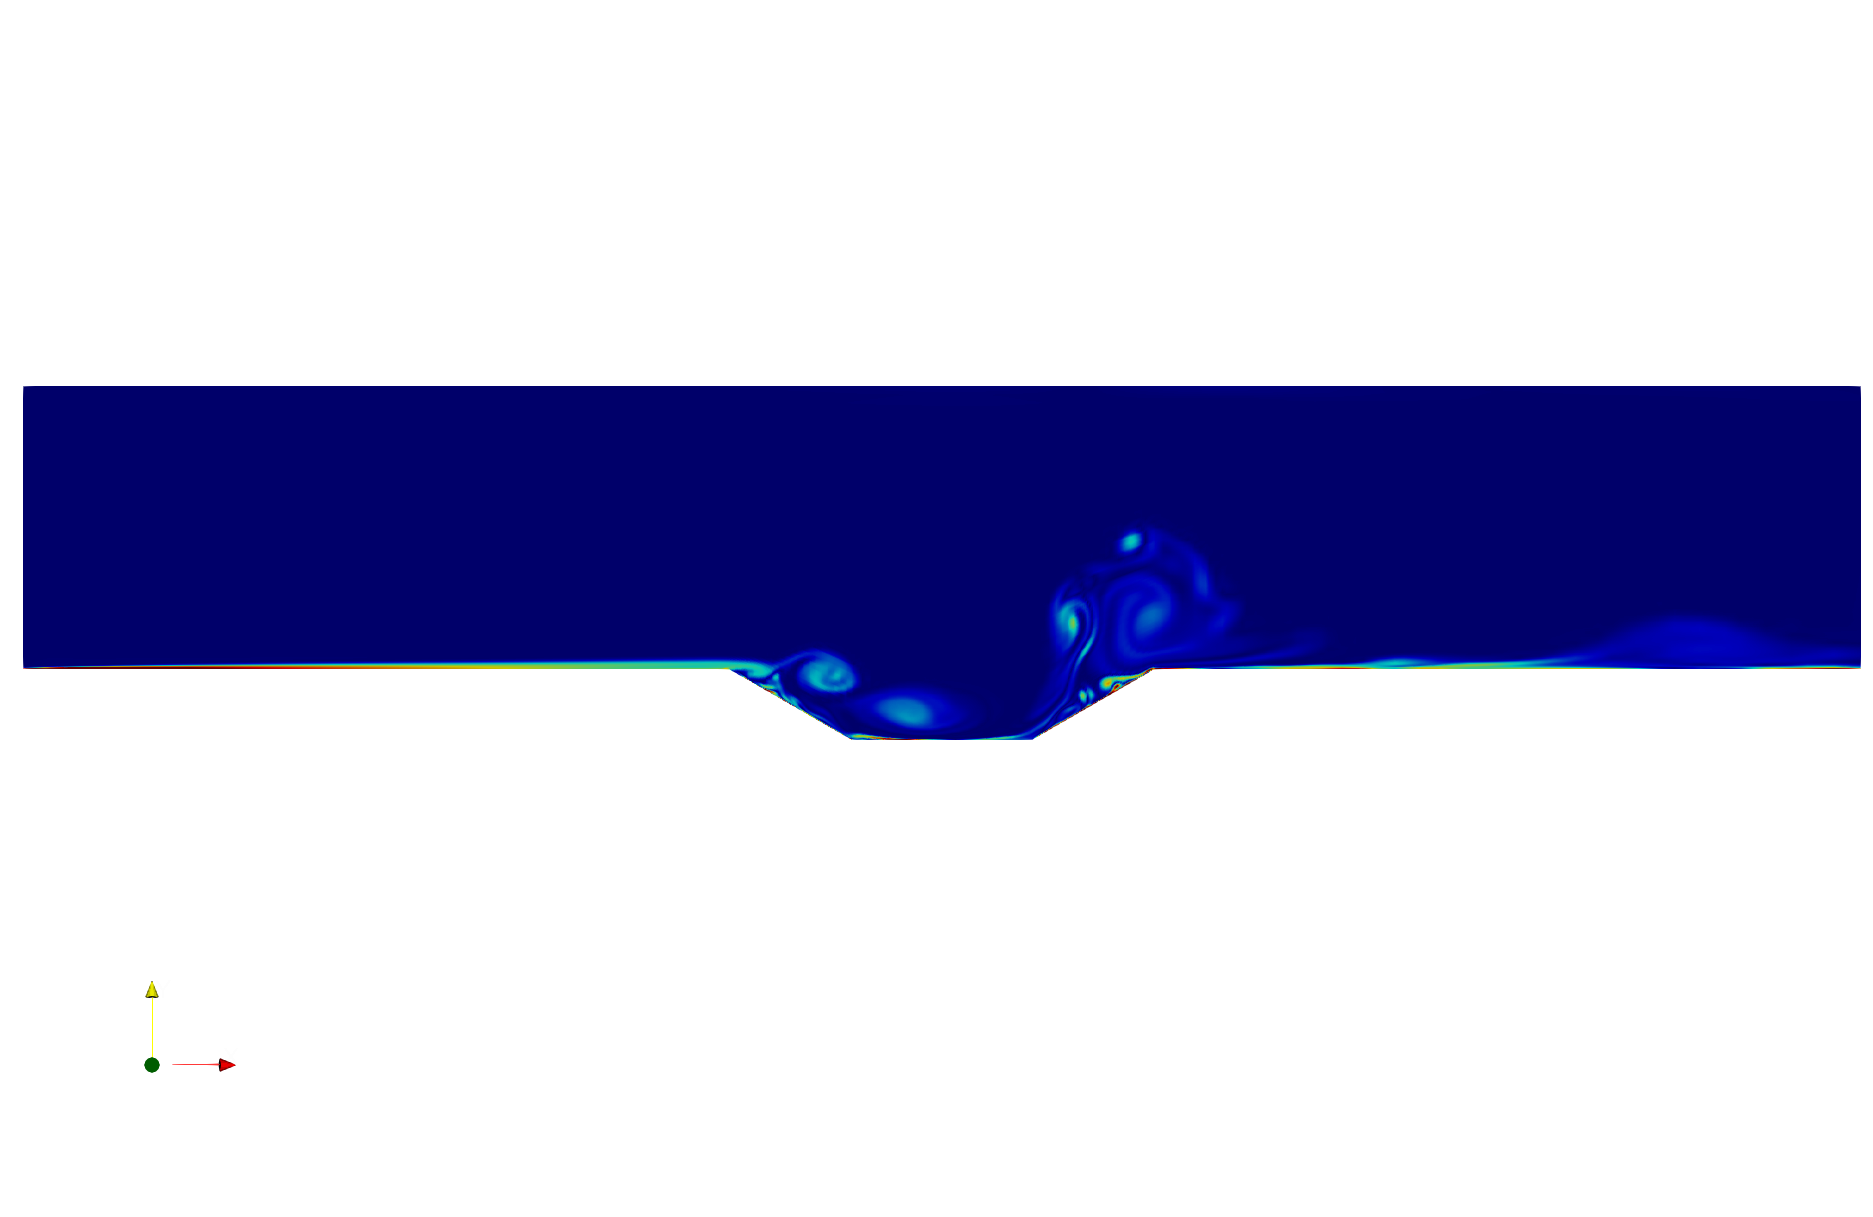
\includegraphics[trim={18cm 16cm 18cm 15cm},clip,width=1.0\linewidth]{figs/cavity/animate/sol0000.png}
\caption{$t=0.0$}
\end{subfigure}
\begin{subfigure}[t]{0.49\textwidth}
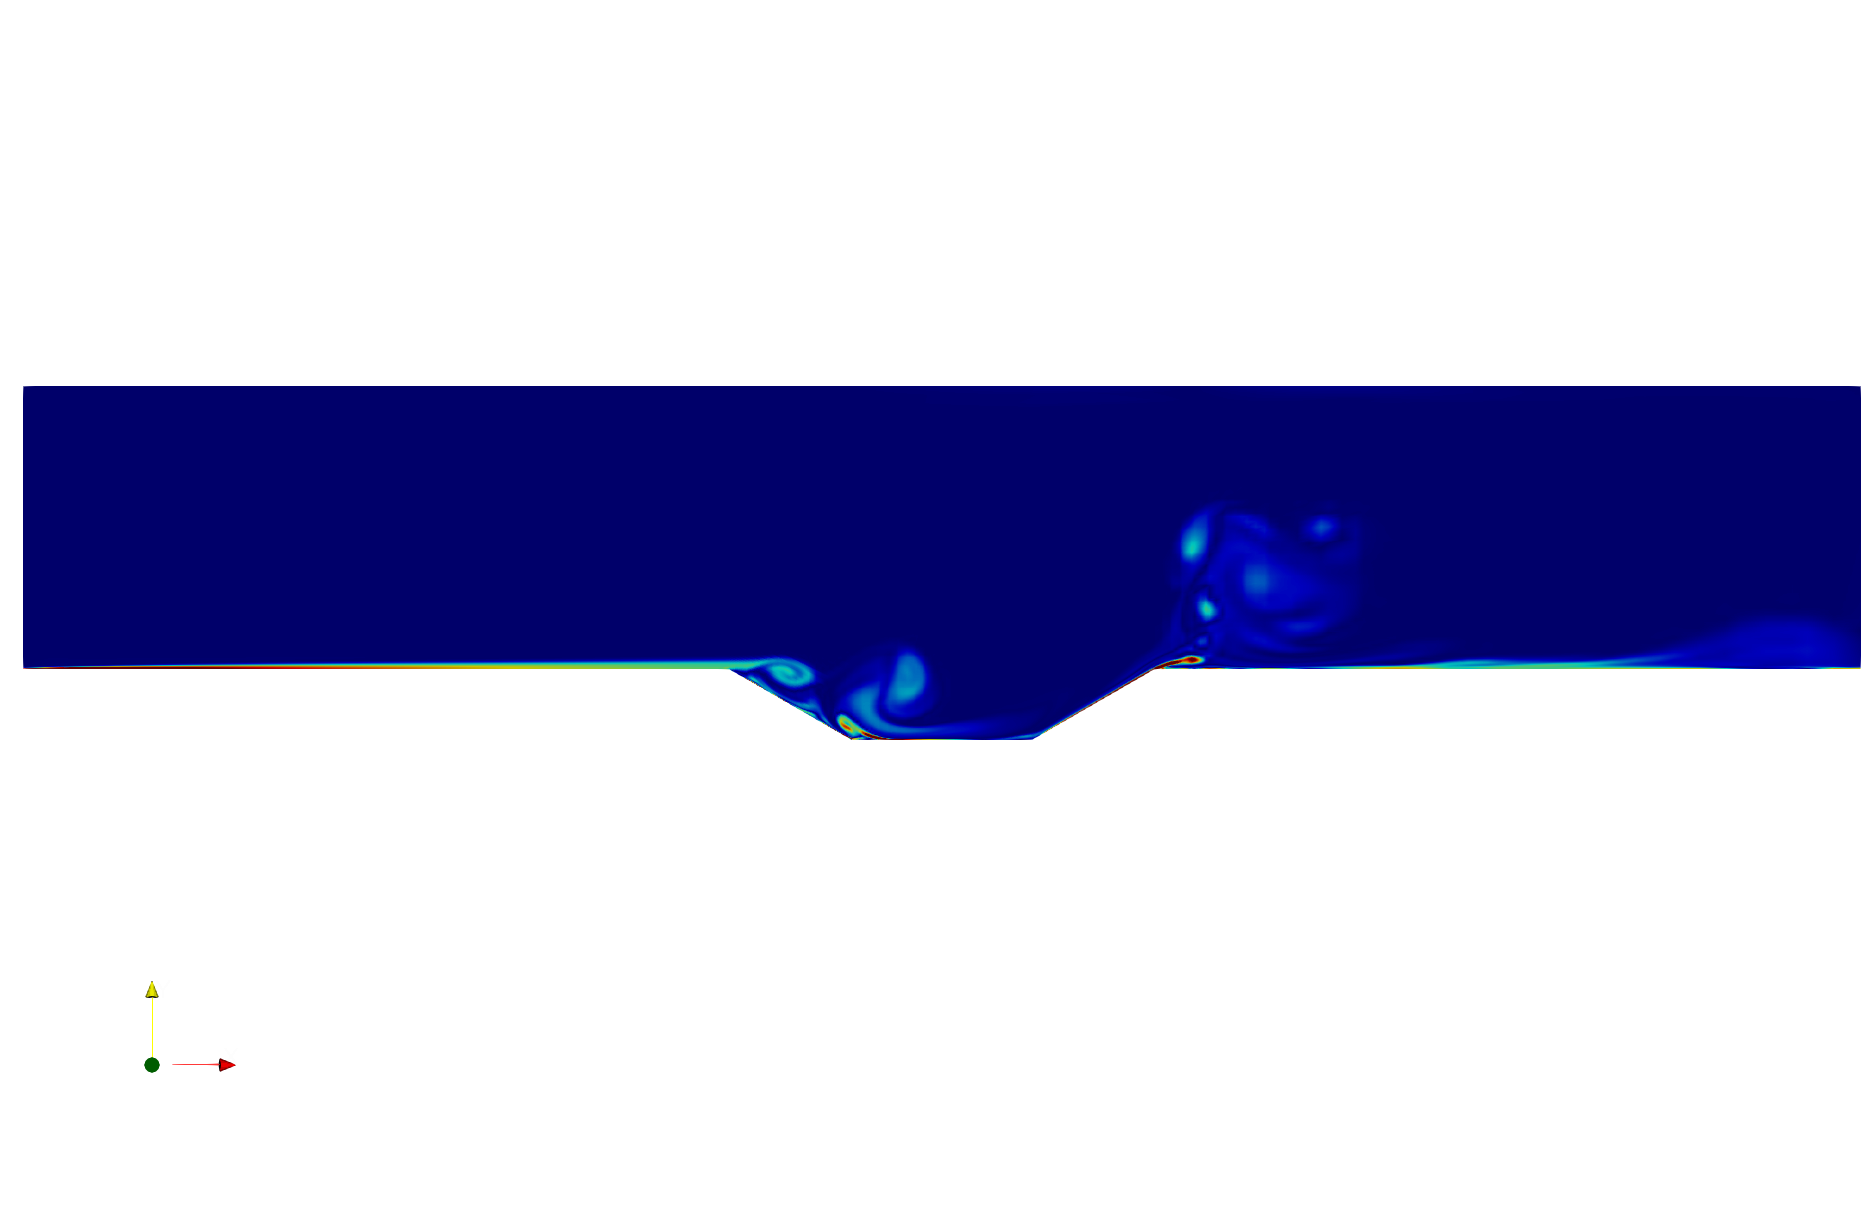
\includegraphics[trim={18cm 16cm 18cm 15cm},clip,width=1.0\linewidth]{figs/cavity/animate/sol0040.png}
\caption{$t=4.0$}
\end{subfigure}
\begin{subfigure}[t]{0.49\textwidth}
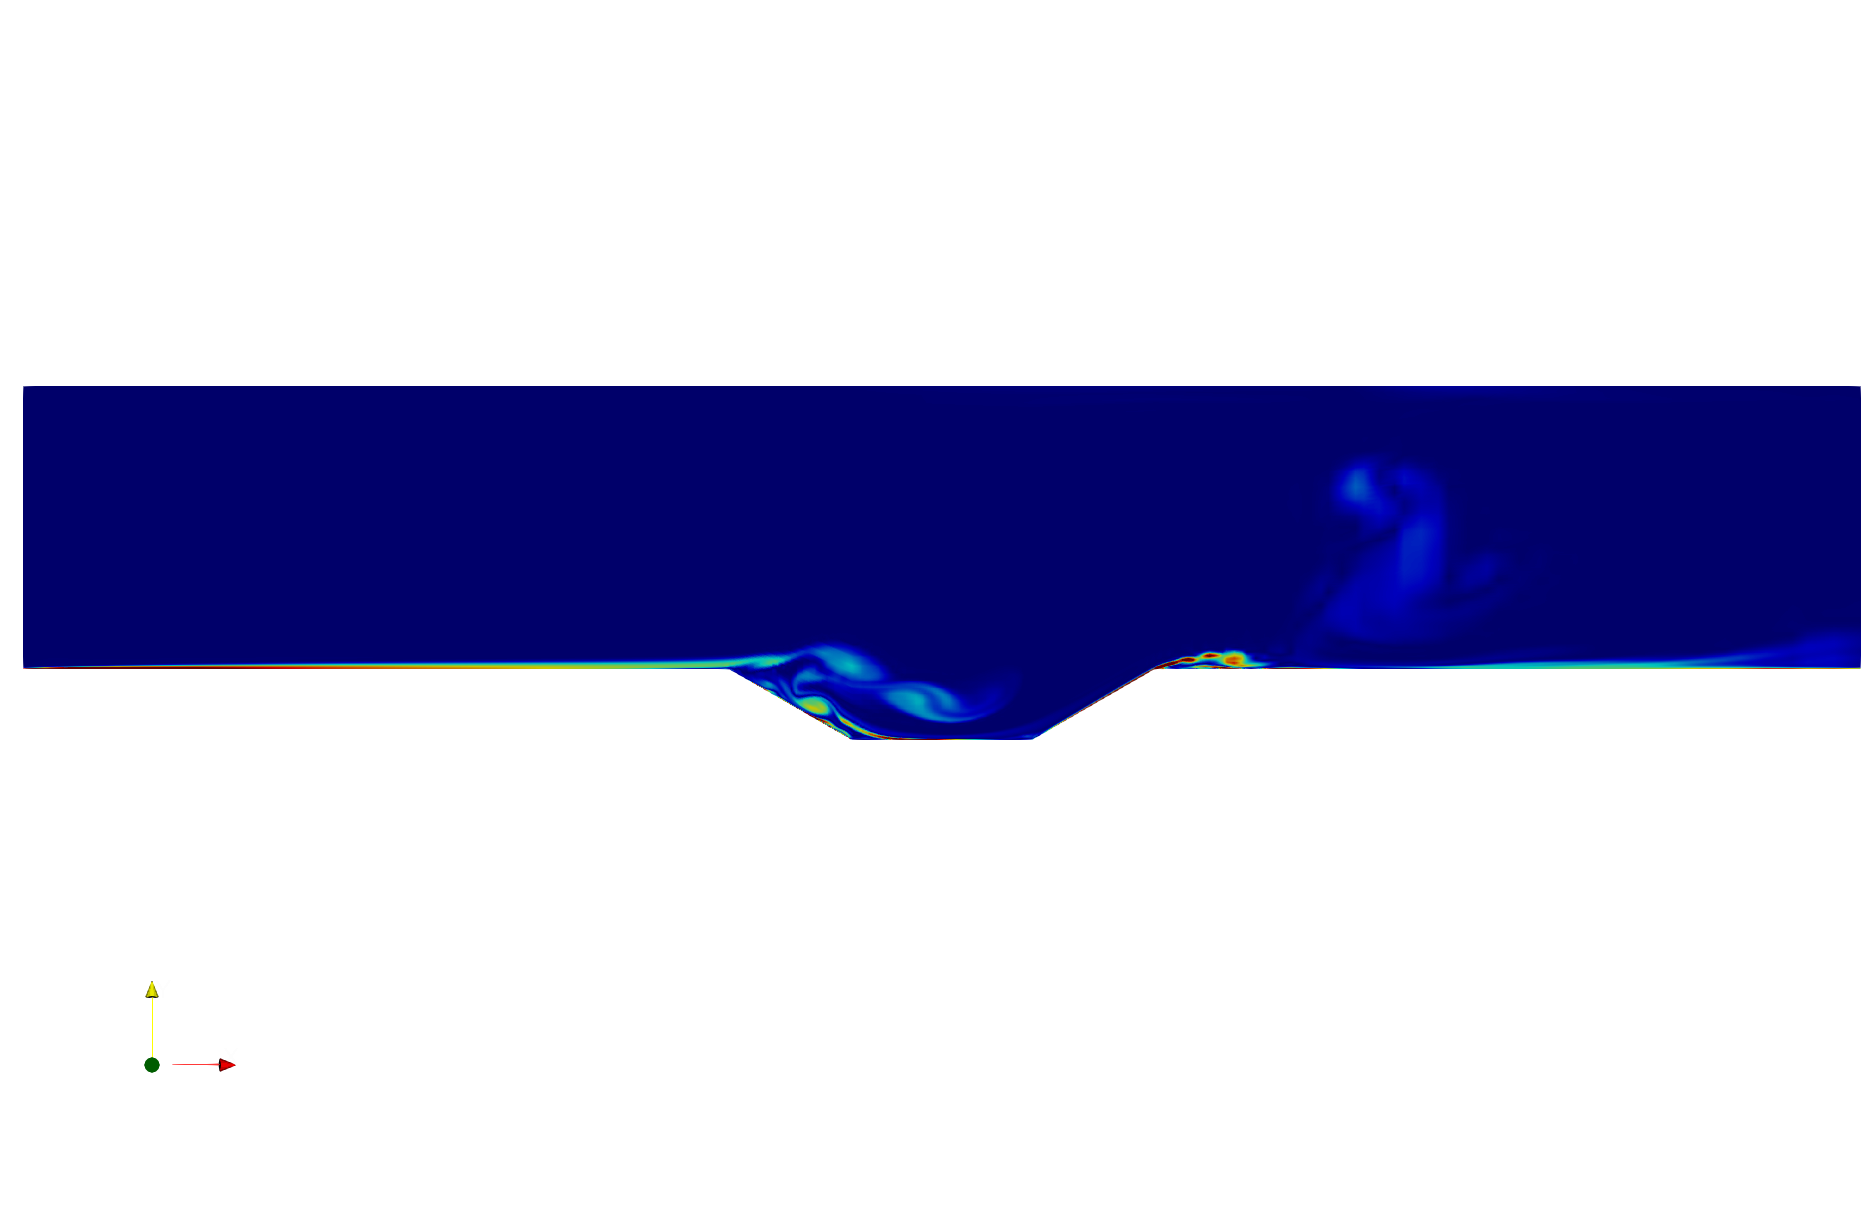
\includegraphics[trim={18cm 16cm 18cm 15cm},clip,width=1.0\linewidth]{figs/cavity/animate/sol0080.png}
\caption{$t=8.0$}
\end{subfigure}
\begin{subfigure}[t]{0.49\textwidth}
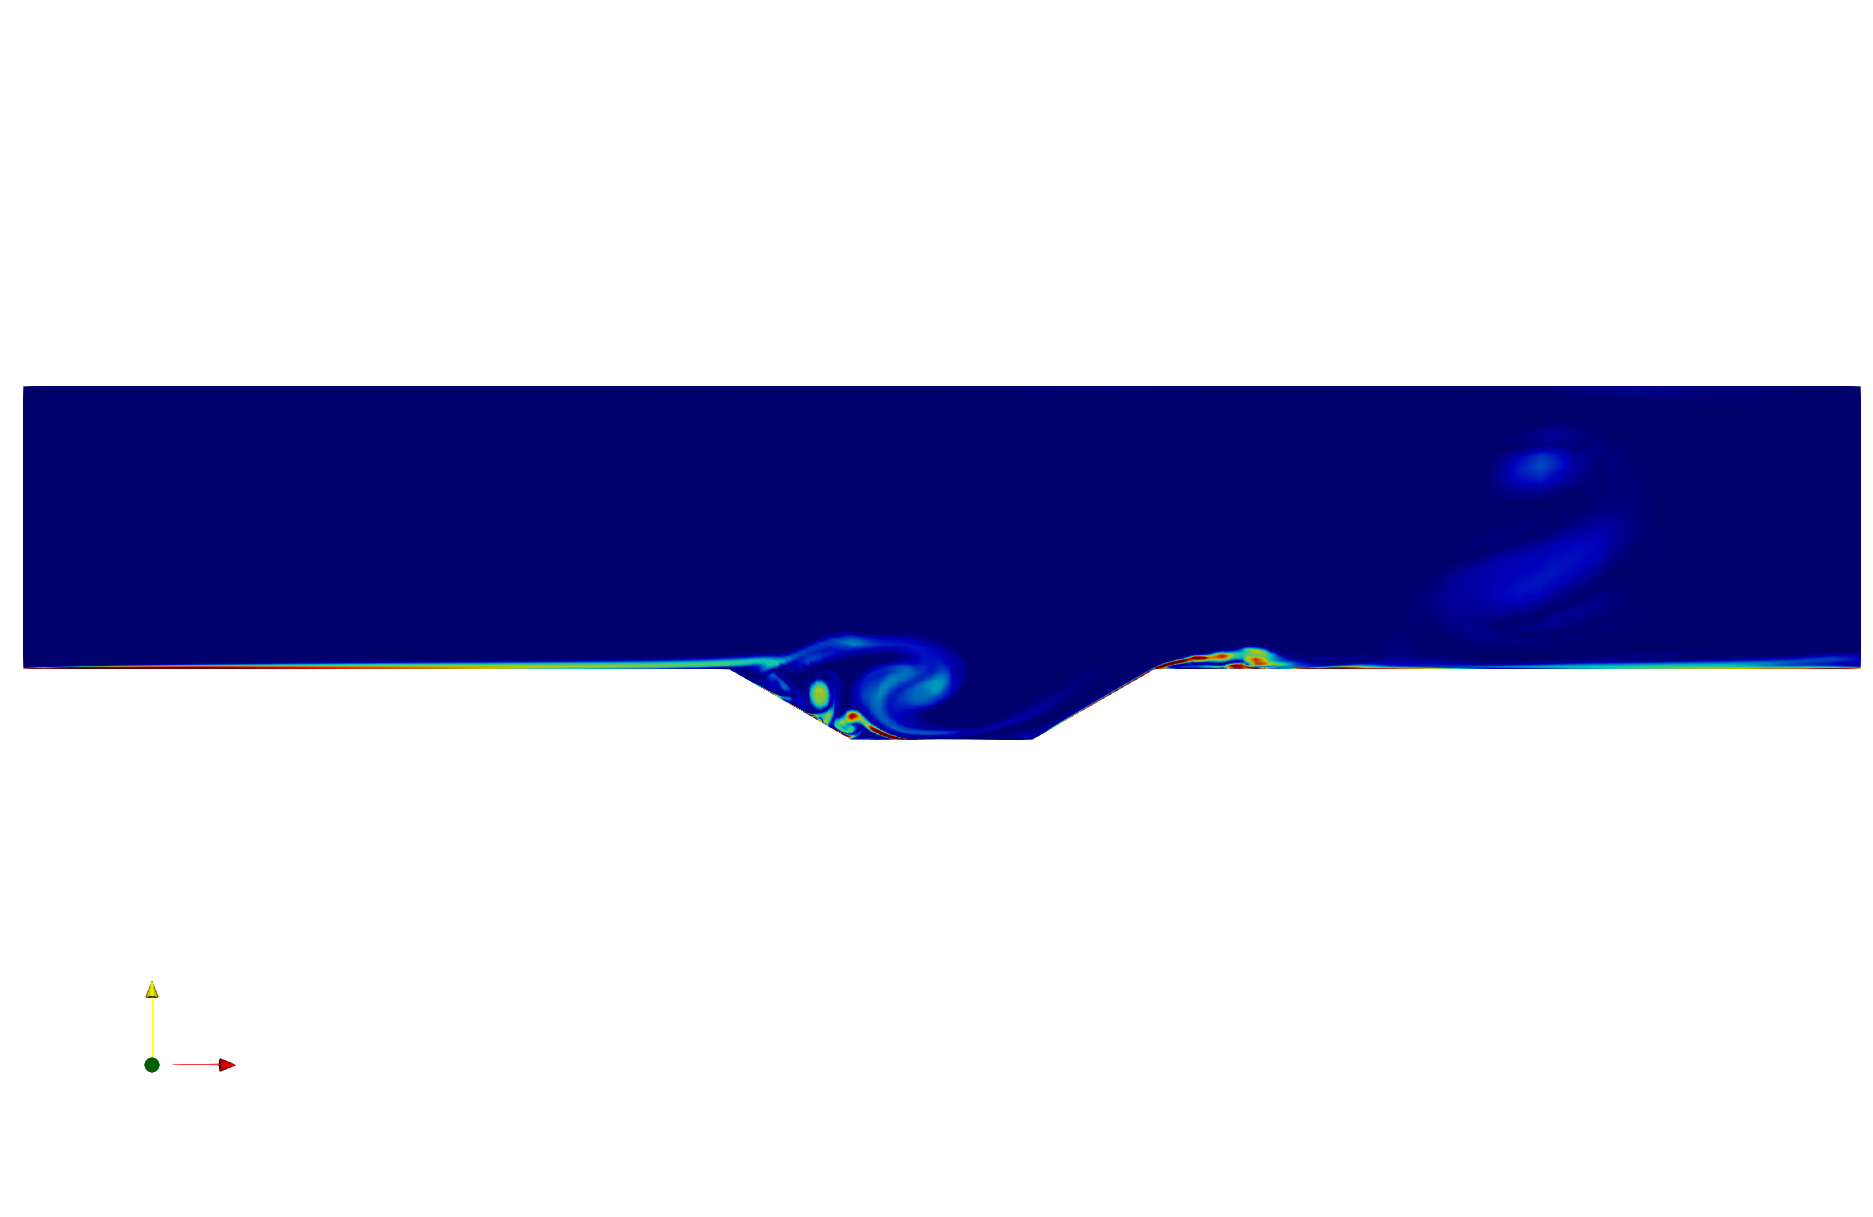
\includegraphics[trim={18cm 16cm 18cm 15cm},clip,width=1.0\linewidth]{figs/cavity/animate/sol0120.png}
\caption{$t=12.0$}
\end{subfigure}
\begin{subfigure}[t]{0.49\textwidth}
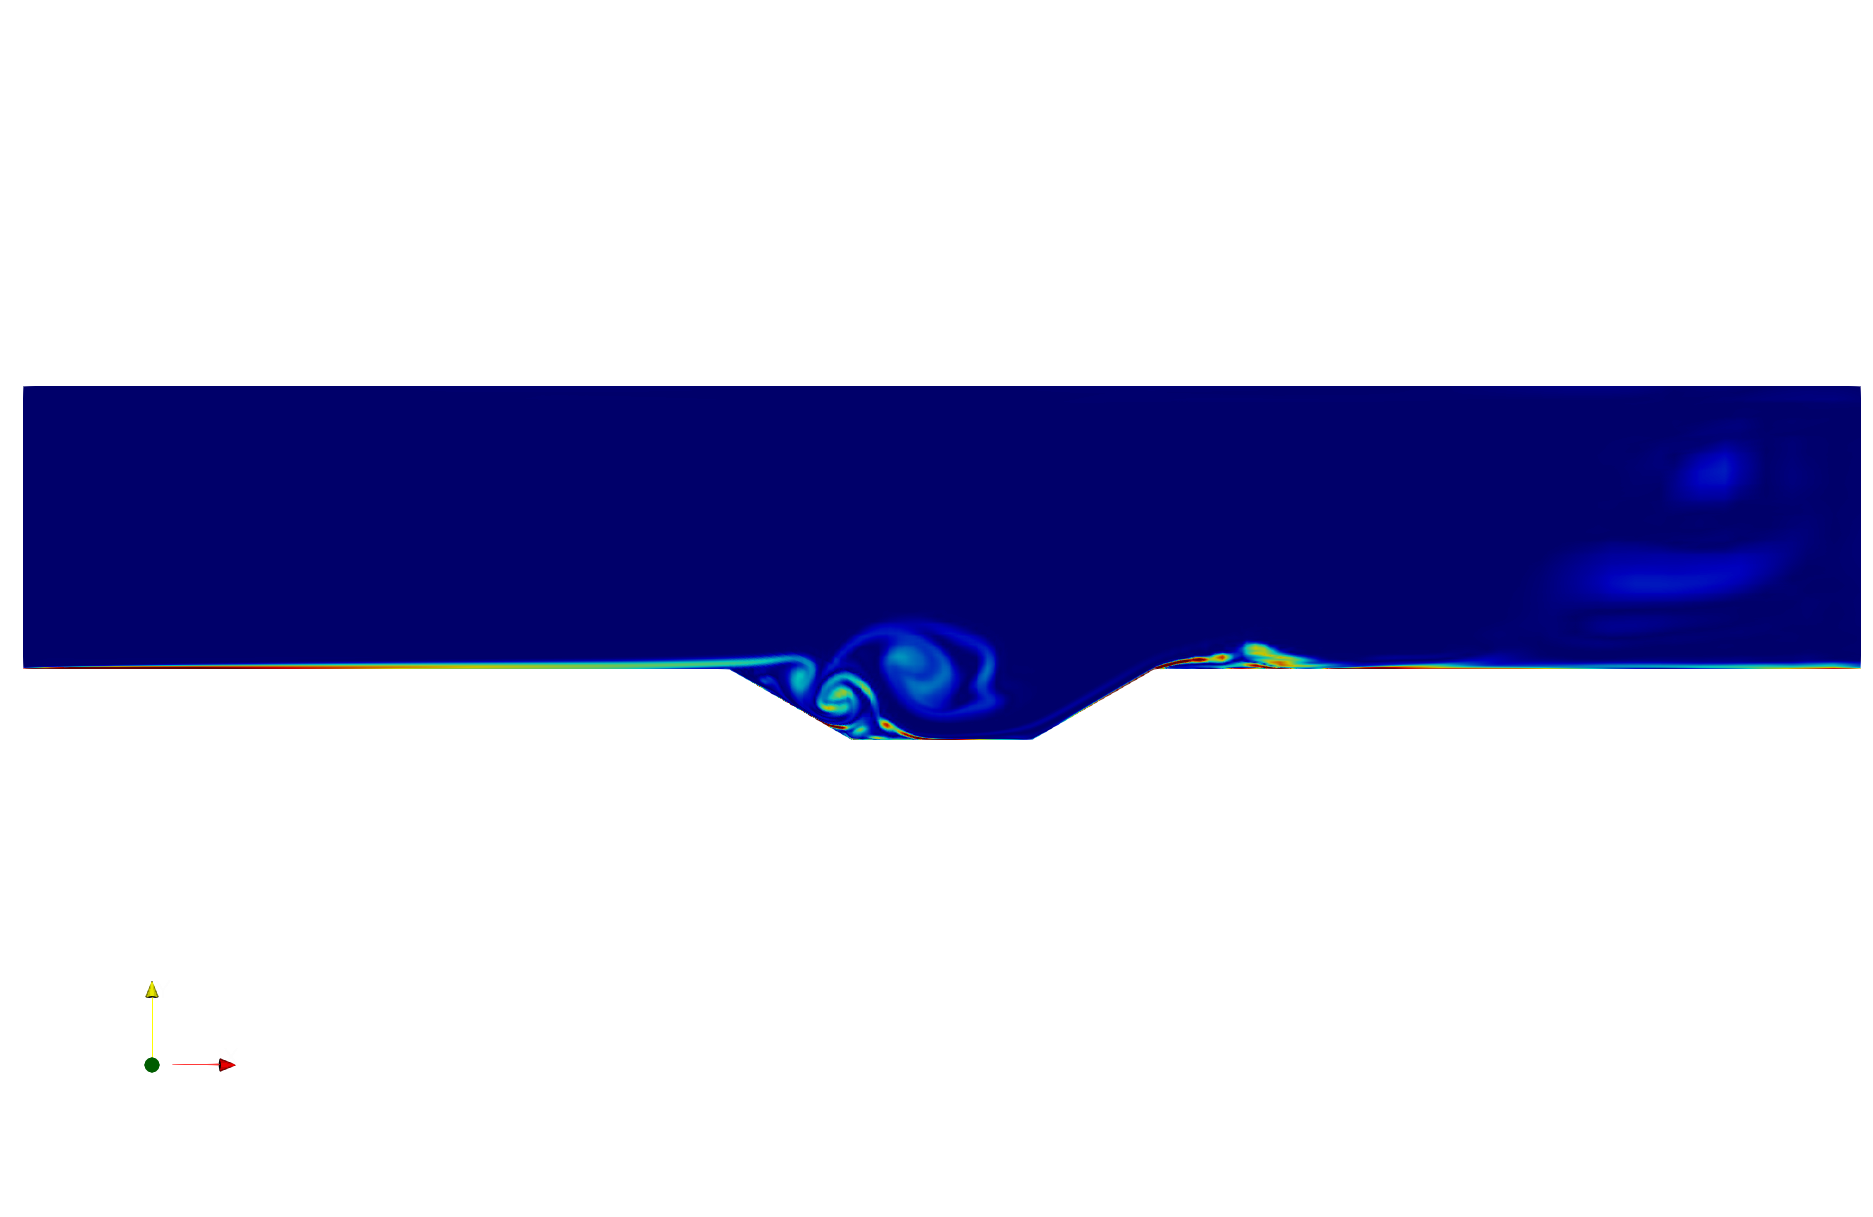
\includegraphics[trim={18cm 16cm 18cm 15cm},clip,width=1.0\linewidth]{figs/cavity/animate/sol0160.png}
\caption{$t=16.0$}
\end{subfigure}
\begin{subfigure}[t]{0.49\textwidth}
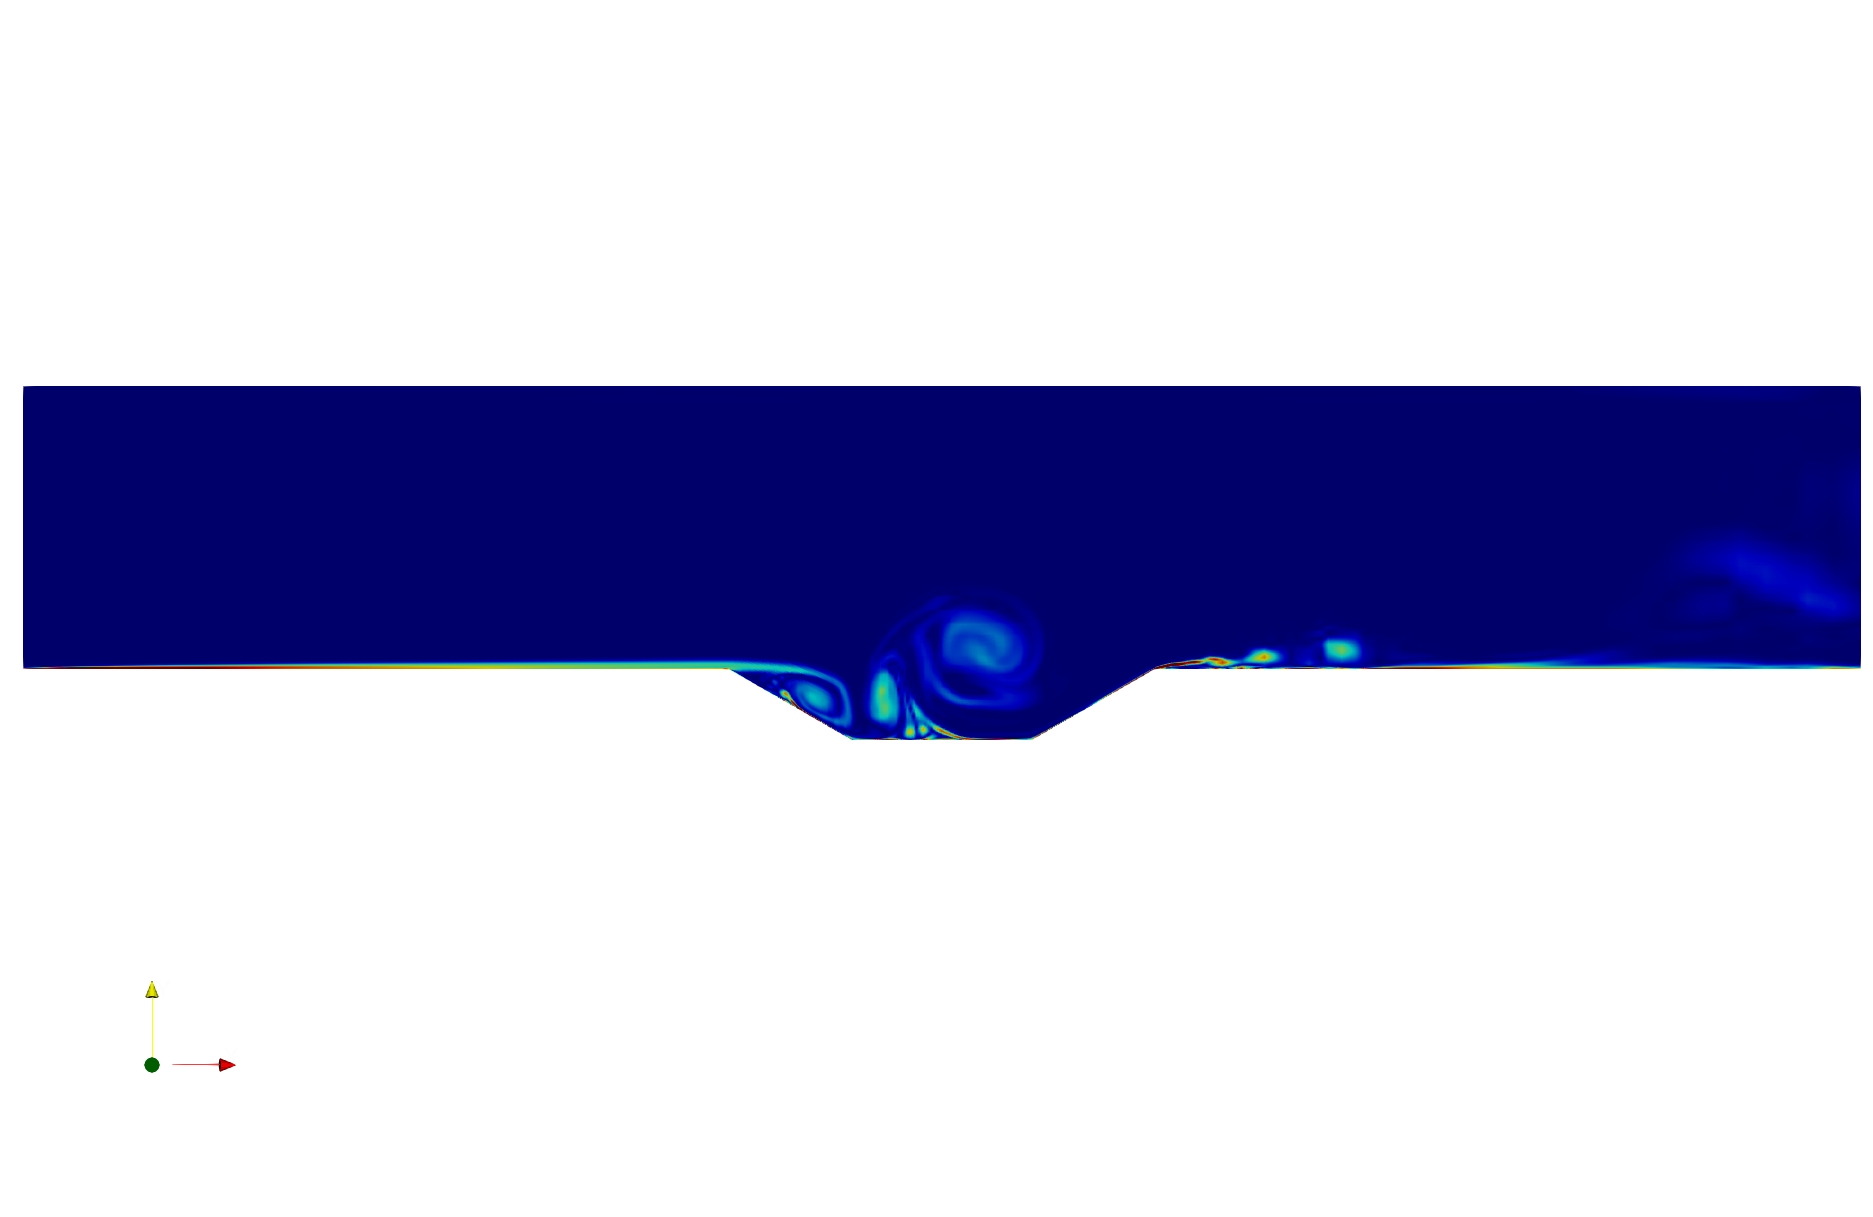
\includegraphics[trim={18cm 16cm 18cm 15cm},clip,width=1.0\linewidth]{figs/cavity/animate/sol0200.png}
\caption{$t=20.0$}
\end{subfigure}
\caption{Vorticity snapshots from the FOM simulation at various time instances.} 
\label{fig:fom_sols_cav}
\end{center}
\end{figure}


\subsubsection{Numerical Results}
We first assess the performance of \methodAcronymROMs\ with varying window sizes. To this end, we consider \methodAcronymROMs\ with uniform window 
sizes of $\Delta T^n \equiv \Delta T = 0.2,0.5,1.0,$ and $2.0$, along with the Galerkin and LSPG ROMs. Results are first considered for basis \#1 as described in 
Table~\ref{tab:rom_basis_details}. For all ROMs, we evolve 
the solution for $t \in [0,100]$. This comprises the same time interval used to construct the trial space. First, Figure~\ref{fig:cav_results1a} depicts the evolution of the pressure at the bottom wall in the midpoint of the computational domain, while Figure~\ref{fig:cav_results1b} depicts the evolution of the normalized $\elltwo$ state error of the various reduced-order models. Both the hyper-reduced Galerkin and LSPG ROMs blow up/fail to converge within the first several time units. The \methodAcronymROM\ minimizing the residual over a window of size $\Delta T = 0.2$ also fails to converge. The \methodAcronymROMs\ that minimize the residual over window sizes of $\Delta T \ge 0.5$ are seen to all be stable and accurate; the pressure response is well characterized and the normalized state errors are again less than $10\%$. The most notable discrepancy between the \methodAcronymROM\ and FOM solutions is a slight phase difference. 






\begin{figure}
\begin{center}

\begin{subfigure}[t]{0.95\textwidth}
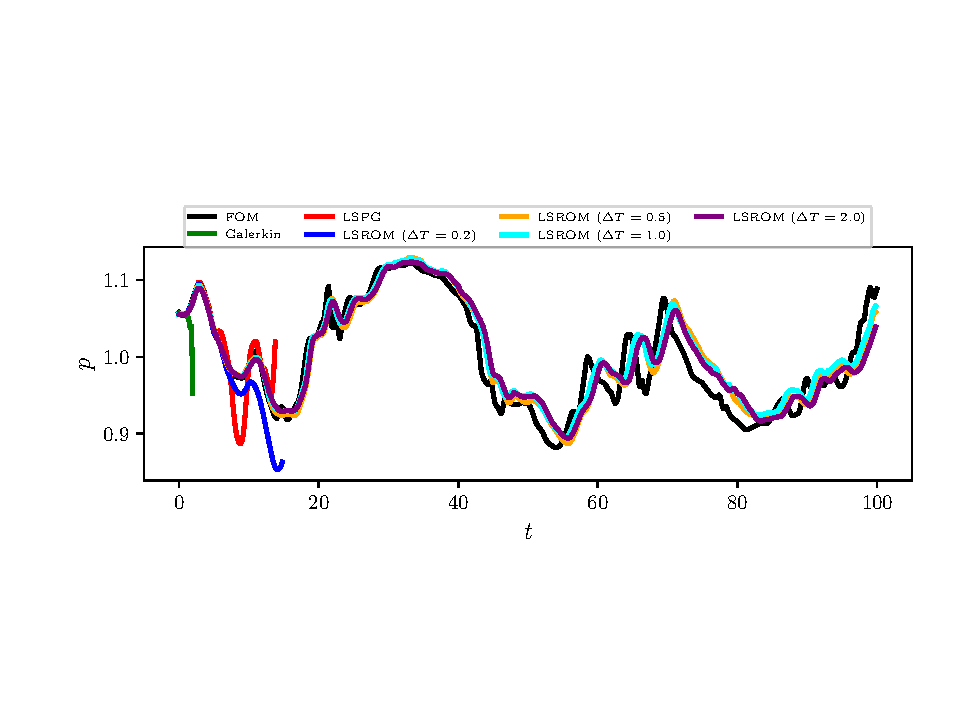
\includegraphics[trim={0cm 3.0cm 0cm 3cm},clip,width=1.\linewidth]{figs/cavity/pressure_basis2.pdf}
\caption{Pressure} 
\label{fig:cav_results1a}
\end{subfigure}

\begin{subfigure}[t]{0.95\textwidth}
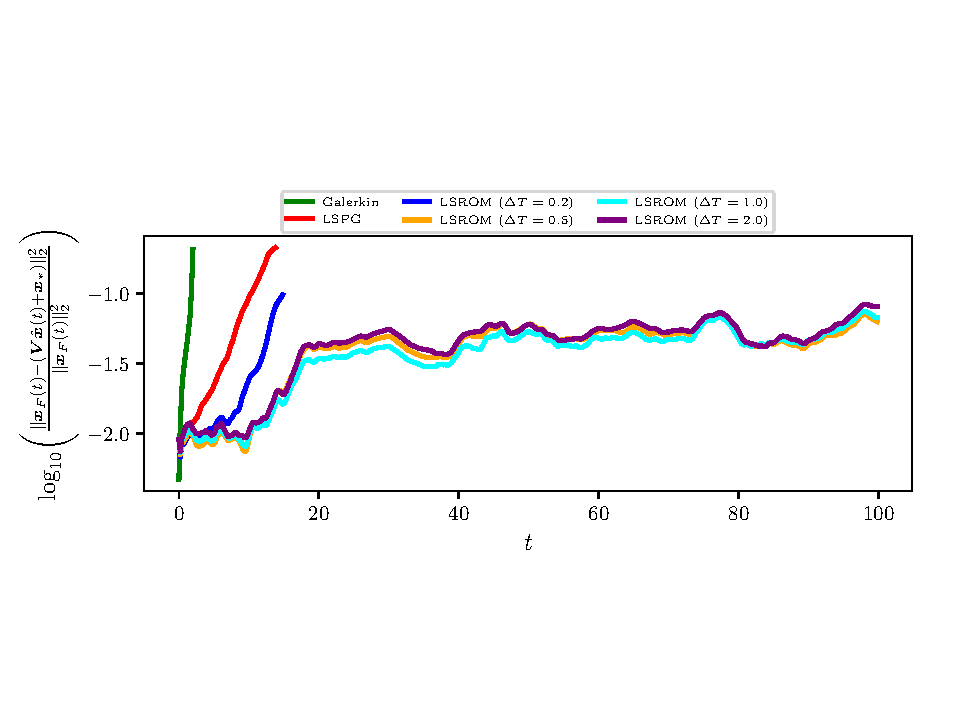
\includegraphics[trim={0cm 2.8cm 0cm 3cm},clip,width=1.\linewidth]{figs/cavity/error_basis2.pdf}
\caption{Normalized $\elltwo$ error}
\label{fig:cav_results1b}
\end{subfigure}

\end{center}
\caption{Comparison of the pressure profiles obtained at the midpoint of the bottom wall (top) and normalized $\elltwo$ state errors (bottom) of various hyper-reduced ROMs to the full-order model solution.}
\label{fig:cav_results1}
\end{figure}

Figure~\ref{fig:cav_results2} shows the integrated error and objective function of the stable \methodAcronymROMs. It is seen that growing the window size over 
which the residual is minimized leads to a lower space--time residual, but not necessarily a lower $\elltwo$ error. This result is consistent with the previous numerical example. Next, Figure~\ref{fig:cav_wallclock}
shows the wall-clock times of the \methodAcronymROMs\ for $t \in [0,10]$ as compared to the LSPG ROM\footnote{Note that LSPG blew up at $t \approx 16.0$, so we focus on the first ten time units}. As expected, increasing the time-slab size again leads to an increase in computational cost. Minimizing the residual over a time-slab comprising 20 time-steps leads to a 2.5x increase in cost over LSPG. 


\begin{figure}
\begin{center}
\begin{subfigure}[t]{0.45\textwidth}
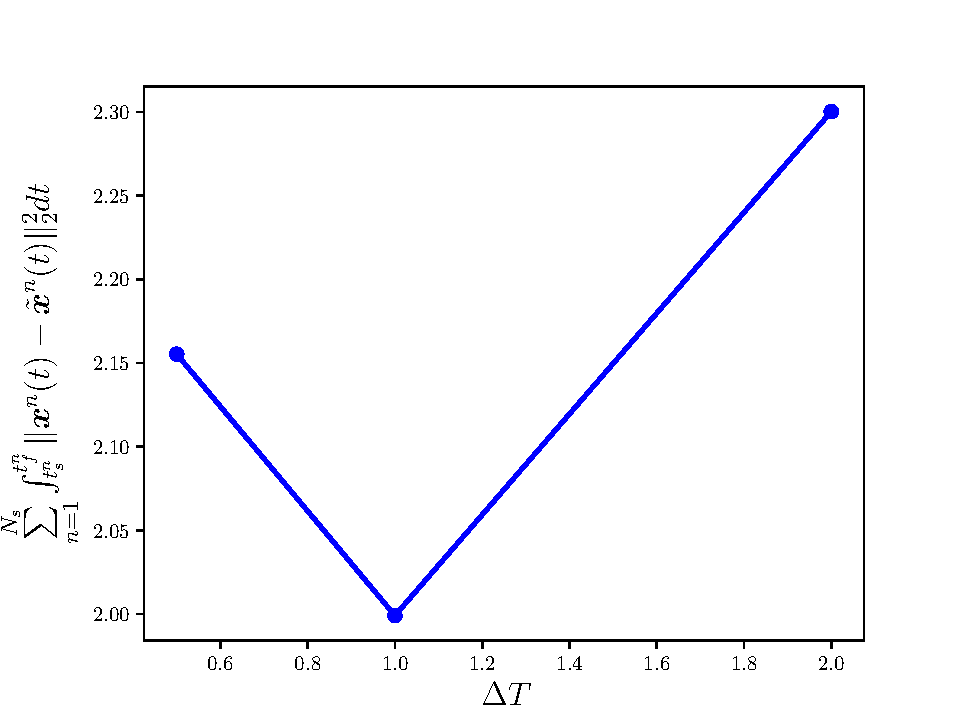
\includegraphics[trim={0cm 0cm 0cm 0cm},clip,width=1.\linewidth]{figs/cavity/error_vs_window_basis2.pdf}
\caption{Integrated $\elltwo$ error}
\label{fig:cav_results2a}
\end{subfigure}
\begin{subfigure}[t]{0.45\textwidth}
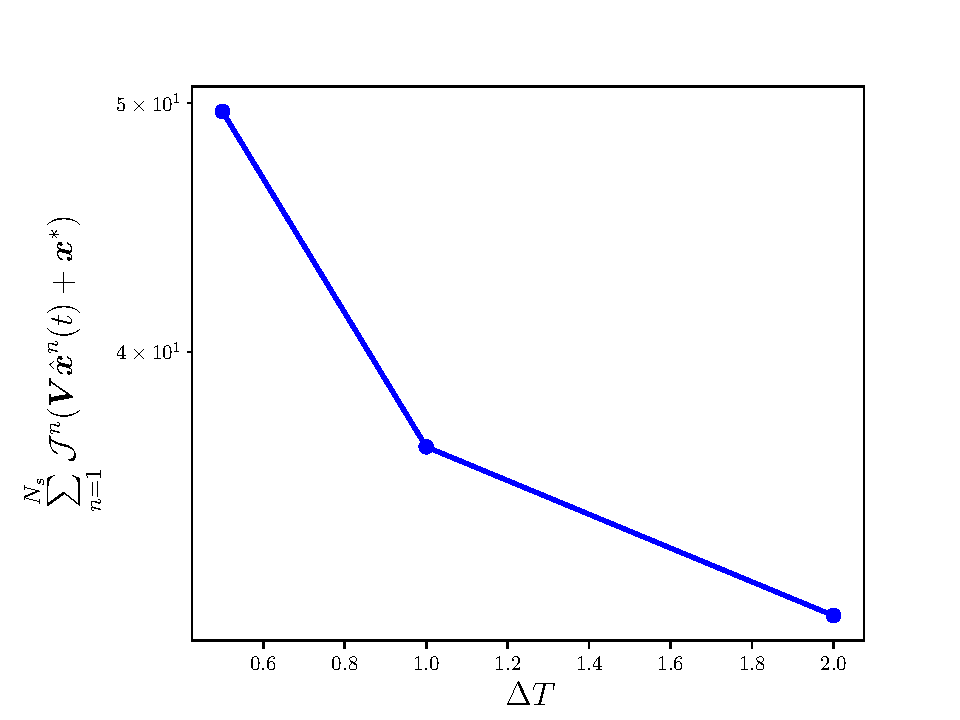
\includegraphics[trim={0cm 0cm 0cm 0cm},clip,width=1.\linewidth]{figs/cavity/objective_vs_window_basis2.pdf}
\caption{Objective function} 
\label{fig:cav_results2b}
\end{subfigure}
\end{center}
\caption{Integrated error (left) and objective function (right) as a function of window size.}
\label{fig:cav_results2}
\end{figure}


\begin{figure}
\begin{center}
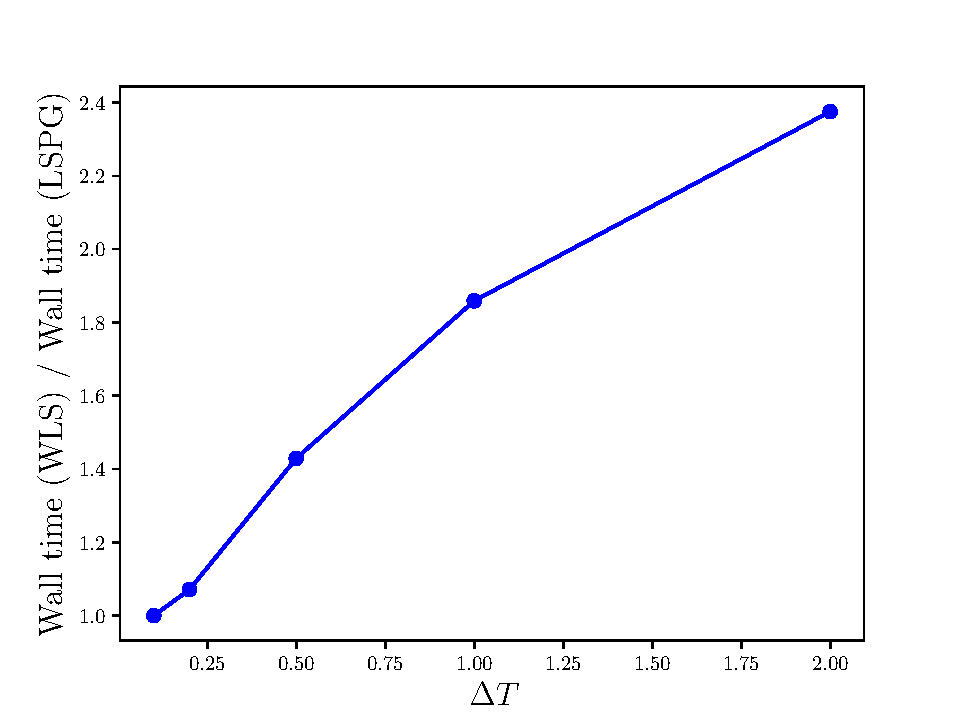
\includegraphics[trim={0cm 0cm 0cm 0cm},clip,width=0.49\linewidth]{figs/cavity/walltime_vs_window_compare_basis2.pdf}
\caption{Wall-clock times of \methodAcronymROMs\ with respect to the LSPG ROM}
\label{fig:cav_wallclock}
\end{center}
\end{figure}

Figure~\ref{fig:cav_snapshots} shows vorticity fields for the FOM, LSPG ROM, and \methodAcronymROM\ with $\Delta T = 0.5$ for the time instance $t = 5.0$. LSPG is observed to exhibit artificial oscillations; the Gauss-Newton method fails to converge at $t \approx 16.0$. The \methodAcronymROM\ at $\Delta T = 0.5$ is able to capture the important features of the flow, including the points of flow separation at the start and end of the ramp, and remains stable for the entire time interval.  

\begin{figure}
\begin{center}
\begin{subfigure}[t]{0.95\textwidth}
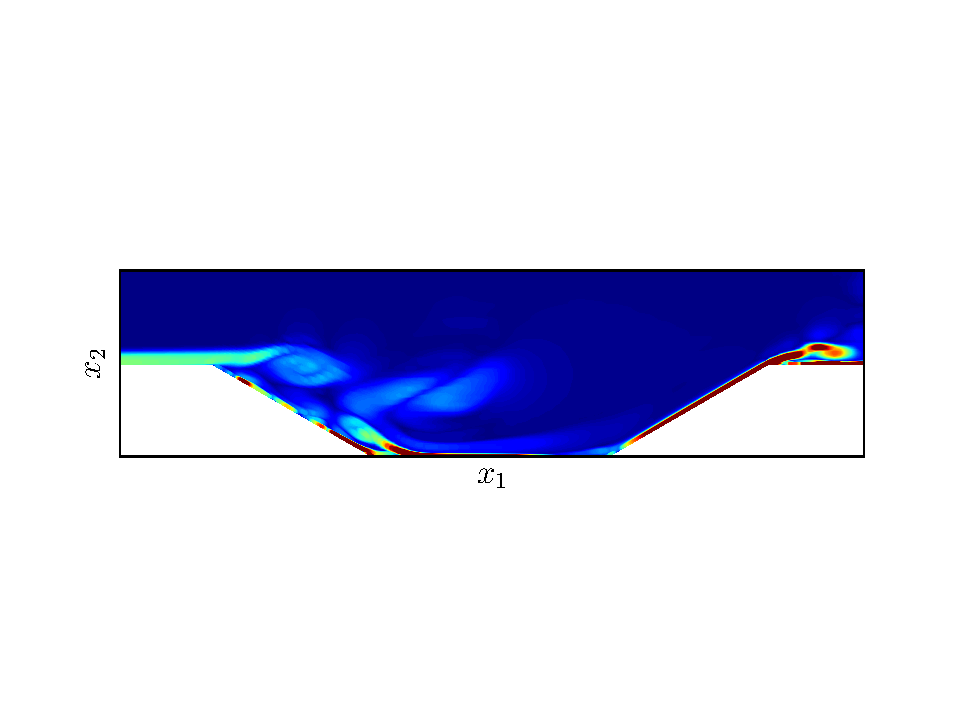
\includegraphics[trim={0cm 3.9cm 0cm 3.9cm},clip,width=1.\linewidth]{figs/cavity/u_fom_t5_basis2.pdf}
\caption{FOM} 
\end{subfigure}
%\begin{subfigure}[t]{0.95\textwidth}
%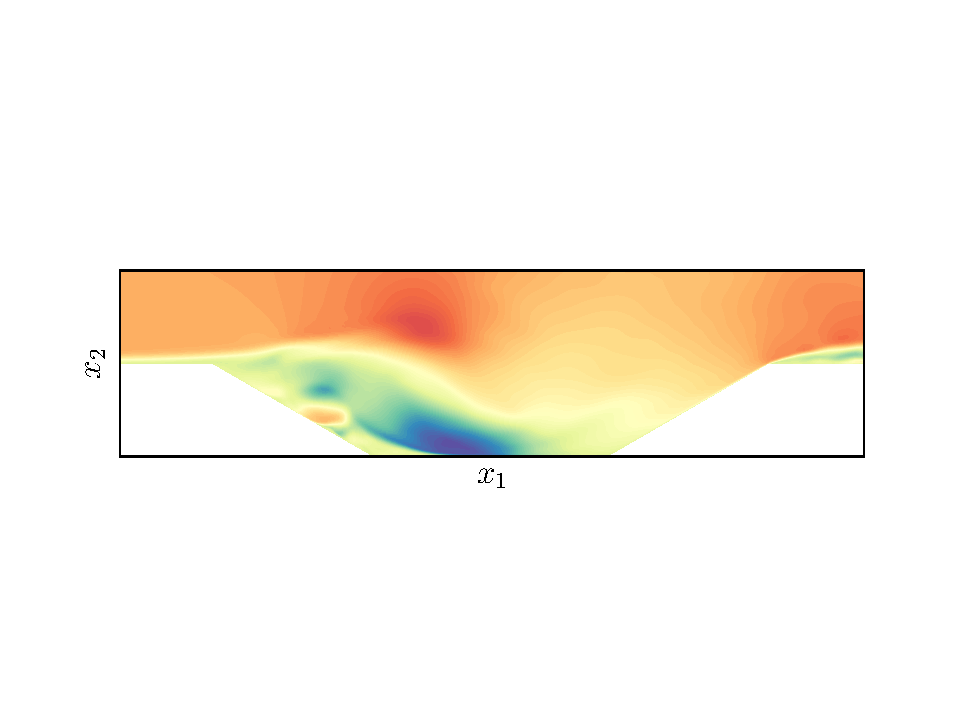
\includegraphics[trim={0cm 3.9cm 0cm 3.9cm},clip,width=1.\linewidth]{figs/cavity/u_c2_t10.pdf}
%\caption{\methodAcronym, $\Delta T = 0.2$} 
%\end{subfigure}
\begin{subfigure}[t]{0.95\textwidth}
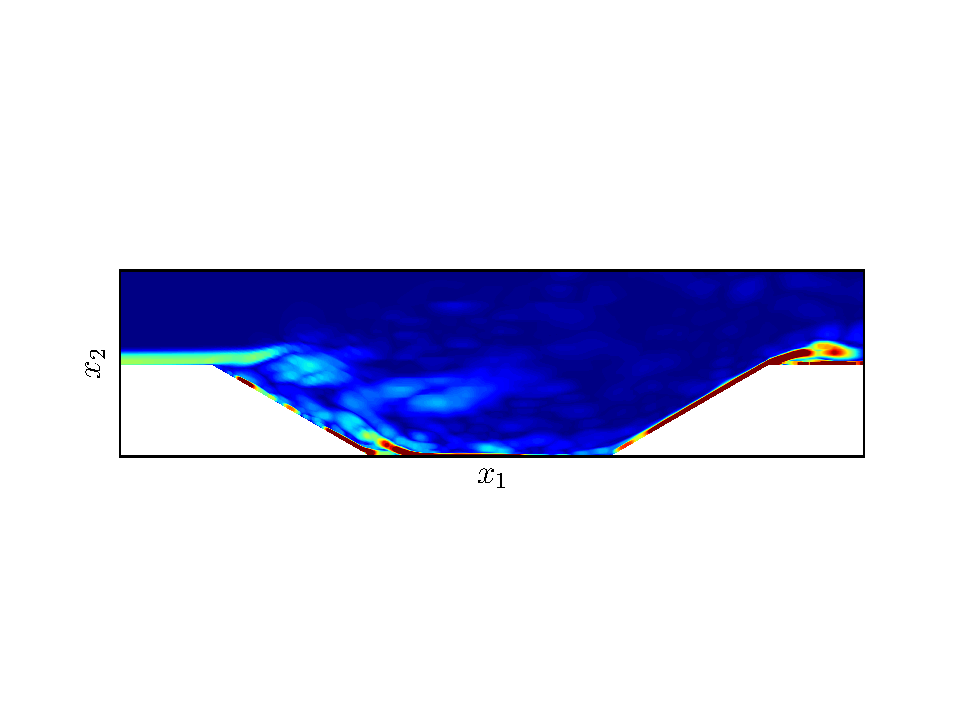
\includegraphics[trim={0cm 3.9cm 0cm 3.9cm},clip,width=1.\linewidth]{figs/cavity/u_lspg_t5_basis2.pdf}
\caption{LSPG} 
\end{subfigure}
\begin{subfigure}[t]{0.95\textwidth}
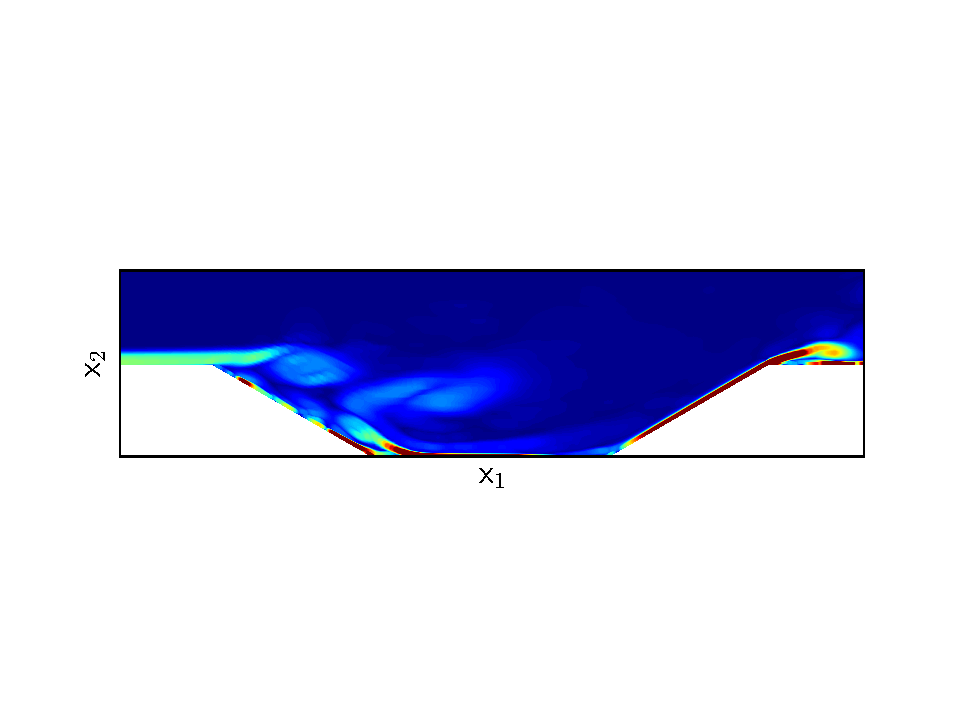
\includegraphics[trim={0cm 3.9cm 0cm 3.9cm},clip,width=1.\linewidth]{figs/cavity/u_c5_t5_basis2.pdf}
\caption{\methodAcronym, $\Delta T = 0.5$} 
\end{subfigure}
%\begin{subfigure}[t]{0.95\textwidth}
%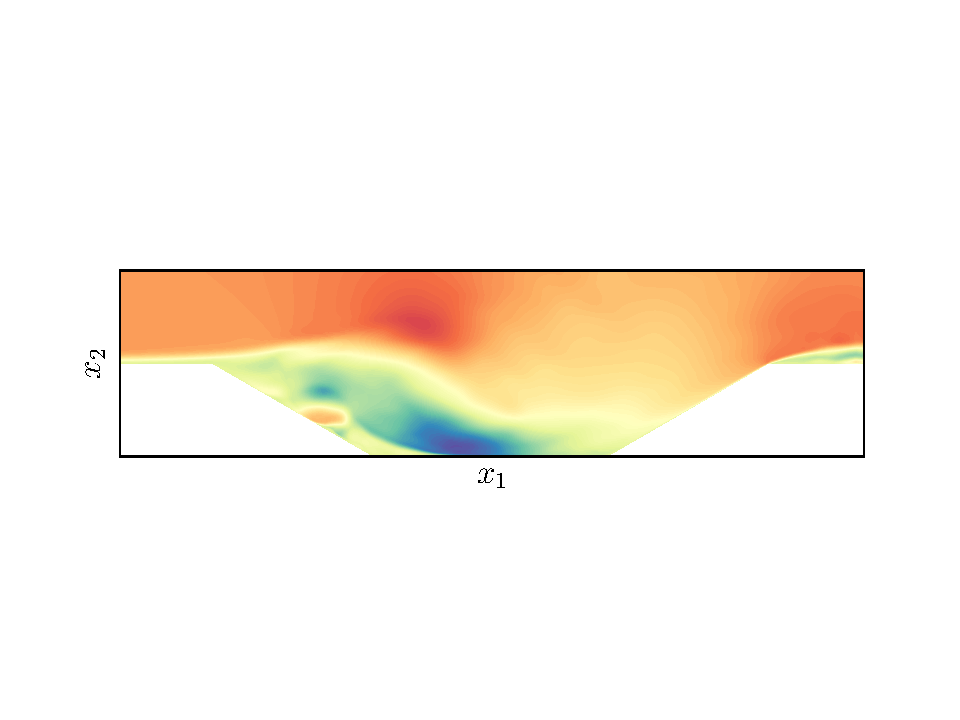
\includegraphics[trim={0cm 3.9cm 0cm 3.9cm},clip,width=1.\linewidth]{figs/cavity/u_c10_t10.pdf}
%\caption{\methodAcronym, $\Delta T = 2.0$} 
%\end{subfigure}
\caption{Field solutions for the vorticity at $t = 5.0$}
\label{fig:cav_snapshots}
\end{center}
\end{figure}


Next, we assess the performance of the various ROMs for basis \#2 as described in Table~\ref{tab:rom_basis_details}, which comprises a richer spatial basis.
 Figure~\ref{fig:cav_results1_basis1} shows the same pressure and error profiles as Figure~\ref{fig:cav_results1}, but for the enriched basis. The LSPG and Galerkin ROMs blow up faster as compared to Figure~\ref{fig:cav_results1}; LSPG fails to converge around $t \approx 8$ (opposed to $t \approx 16$), while Galerkin blows up almost immediately. The 
\methodAcronymROMs\ again yield improved performance: \methodAcronymROMs\ minimizing the residual over window sizes of $\Delta T \ge 0.5$ are seen to all be stable and accurate; the pressure response is well characterized and the normalized state errors are less than $5\%$. The \methodAcronymROMs\ with $\Delta T \ge 0.5$ leveraging the enriched basis yield more accurate results than \methodAcronymROMs\ using the coarse basis.
 

\begin{figure}
\begin{center}

\begin{subfigure}[t]{0.95\textwidth}
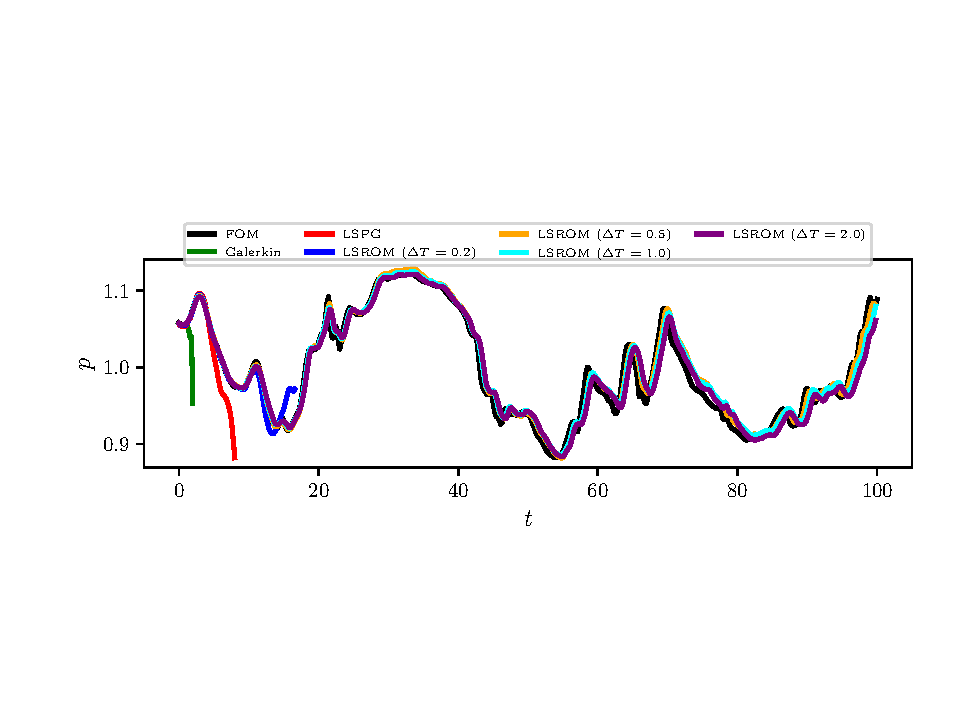
\includegraphics[trim={0cm 2.5cm 0cm 2.5cm},clip,width=1.\linewidth]{figs/cavity/pressure.pdf}
\caption{Pressure} 
\label{fig:cav_results1a_basis1}
\end{subfigure}

\begin{subfigure}[t]{1.0\textwidth}
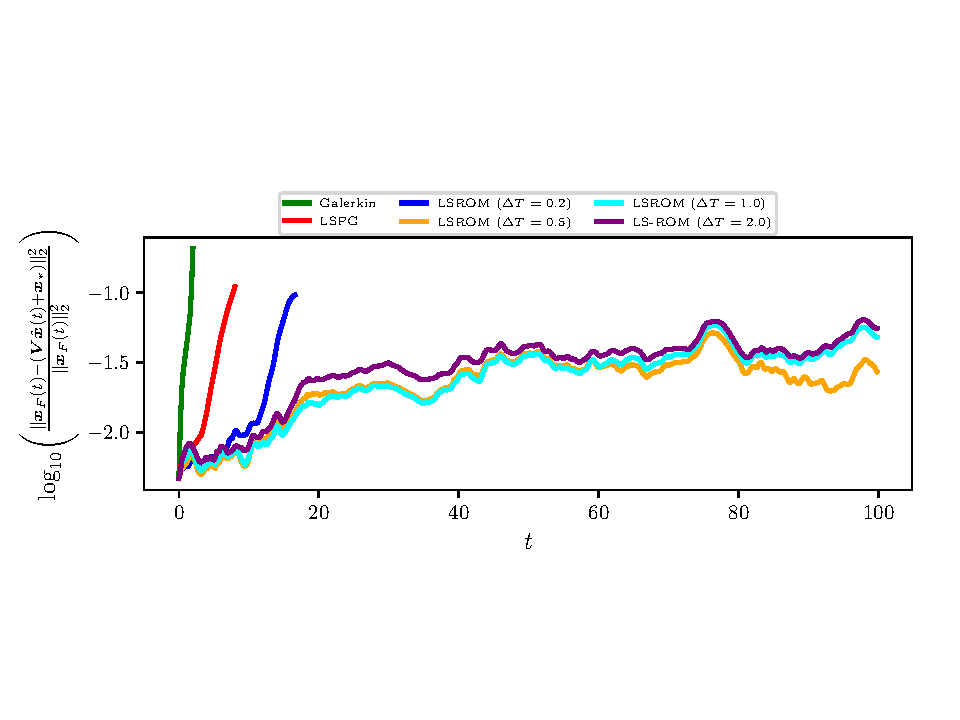
\includegraphics[trim={0cm 2.5cm 0cm 3cm},clip,width=1.\linewidth]{figs/cavity/error.pdf}
\caption{Normalized $\elltwo$ error}
\label{fig:cav_results1b_basis1}
\end{subfigure}
\end{center}
\caption{Comparison of the pressure profiles obtained at the midpoint of the bottom wall (top) and normalized $\elltwo$ state errors (bottom) of various hyper-reduced ROMs to the full-order model solution.}
\label{fig:cav_results1_basis1}
\end{figure}


\begin{figure}
\begin{center}
\begin{subfigure}[t]{0.45\textwidth}
\includegraphics[trim={0cm 0cm 0cm 0cm},clip,width=1.\linewidth]{figs/cavity/error_vs_window.pdf}
\caption{Integrated $\elltwo$ error}
\label{fig:cav_results3a}
\end{subfigure}
\begin{subfigure}[t]{0.45\textwidth}
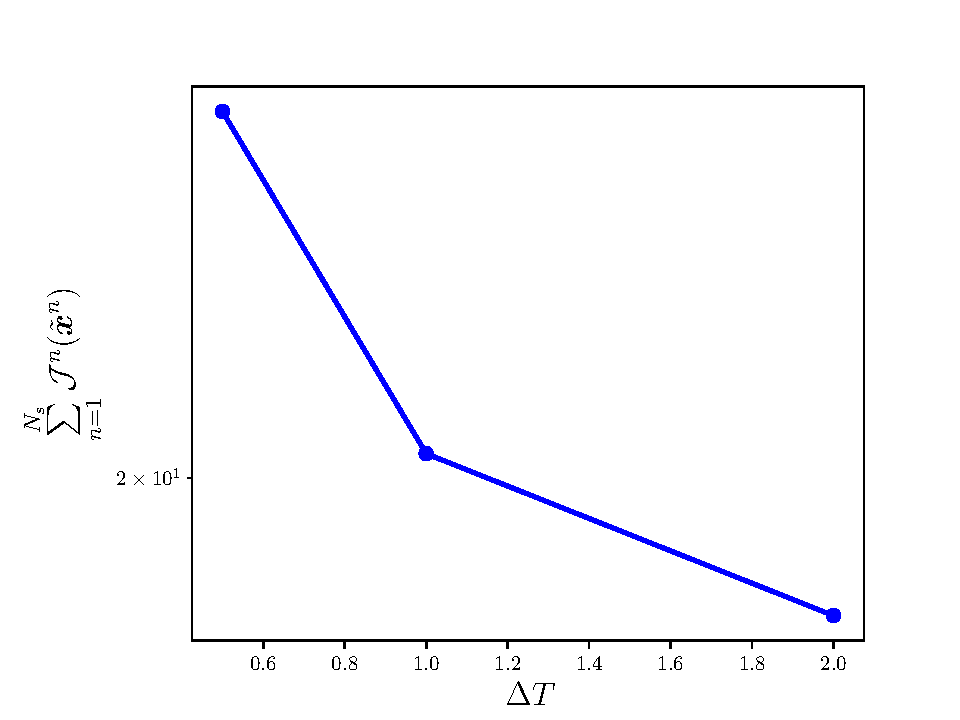
\includegraphics[trim={0cm 0cm 0cm 0cm},clip,width=1.\linewidth]{figs/cavity/objective_vs_window.pdf}
\caption{Objective function} 
\label{fig:cav_results3b}
\end{subfigure}
\end{center}
\caption{Integrated error (left) and objective function (right) as a function of window size.}
\label{fig:cav_results3}
\end{figure}


Finally, Figure~\ref{fig:cav_wallclock} shows the wall-clock times of the \methodAcronymROMs\ as compared to the LSPG ROMs for basis \#2. Increasing the window size again leads to an increase in computational cost. Minimizing the residual over a window comprising 20 time-steps leads to a 2.5x increase in cost over LSPG. This increase in computational cost is particularly reasonable in this example as LSPG yielded an unstable solution. 
\begin{figure}
\begin{center}
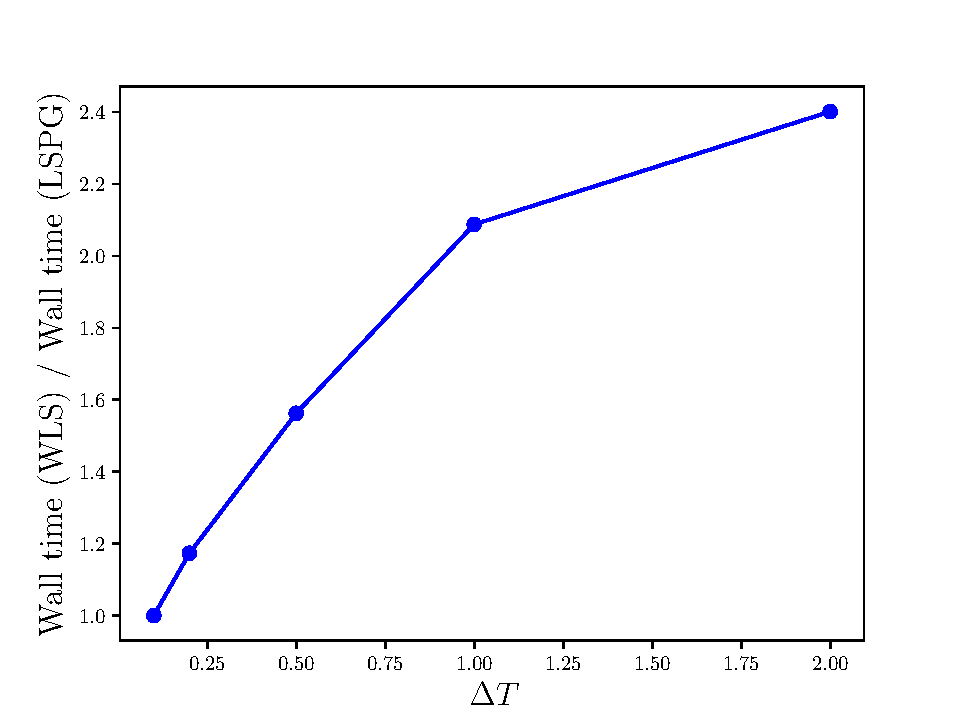
\includegraphics[trim={0cm 0cm 0cm 0cm},clip,width=0.49\linewidth]{figs/cavity/walltime_vs_window_compare.pdf}
\caption{Wall-clock times of \methodAcronymROMs\ with respect to the LSPG ROM.}
\label{fig:cav_wallclock}
\end{center}
\end{figure}


%\begin{figure}
%\begin{center}
%\begin{subfigure}[t]{0.45\textwidth}
%\includegraphics[trim={0cm 0cm 0cm 0cm},clip,width=1.\linewidth]{figs/cavity/error_vs_window.pdf}
%\caption{Integrated $L^2$ error}
%\label{fig:cav_results2a_basis1}
%\end{subfigure}
%\begin{subfigure}[t]{0.45\textwidth}
%\includegraphics[trim={0cm 0cm 0cm 0cm},clip,width=1.\linewidth]{figs/cavity/objective_vs_window.pdf}
%\caption{Objective function} 
%\label{fig:cav_results2b_basis1}
%\end{subfigure}
%\end{center}
%\caption{Integrated error (left) and objective function (right) as a function of window size.}
%\label{fig:cav_results2_basis1}
%\end{figure}





\section{Conclusions}\label{sec:conclude}
This paper proposed the windowed least-squares (\methodAcronym) \approachKwd\ for model reduction  of dynamical systems. The approach sequentially minimizes the
	time-continuous full-order-model residual within a low-dimensional space--time trial
	subspace over time windows. The approach was formulated for two types of trial subspaces: one that reduces only the spatial dimension of the full-order model, and one that reduces both the spatial and temporal dimensions of the full-order model. For each type of trial
	subspace, we outlined two different solution techniques: direct (i.e.,
	discretize then optimize) and indirect (i.e., optimize then discretize). We showed that particular instances of the approach recover Galerkin,
	least-squares Petrov--Galerkin (LSPG), and space–time LSPG projection.  
The case of \spatialAcronym\ trial subspaces is of particular interest in the \methodAcronym\ context: it was shown that indirect methods comprise solving a coupled two-point 
Hamiltonian boundary value problem.
The forward system, which is forced by an auxiliary costate,
		evolves the (spatial) generalized coordinates of the ROM in time. The
		backward system, which is forced by the time-continuous FOM residual
		evaluated about the ROM state, governs the dynamics of the costate. 

Numerical experiments of the compressible Euler and Navier--Stokes equations demonstrated the utility in the proposed approach. The first numerical experiment, in where the Sod shock tube was examined, demonstrated that \methodAcronymROMs\ minimizing the residual over larger time windows yielded solutions with lower space--time residuals. Increasing the window size over which the residual was minimized, however, did not necessarily decrease the solution error in the $\elltwo$-norm; we observed this to occur over an intermediary window size. We additionally observed that the  
\methodAcronym\ \approachKwd\ overcomes the time-discretization sensitivity that LSPG is subject to. The second numerical experiment, which examined collocated ROMs of a compressible cavity flow, demonstrated the utility of the \methodAcronym\ formulation on a more complex flow. In this experiment, \methodAcronymROMs\ yielded predictions with relative errors less than $5-10\%$, while the Galerkin and LSPG ROMs failed to converge/blew up. Increasing the window size over which the residual was minimized again led to a lower space--time residual, but not necessarily a lower error in the $\elltwo$-norm.

%In the case of spatial dimension-reduction-only, \methodAcronym\ displays improved performance over LSPG at the expense of an increased computational cost. This increase in computational cost is due to the fact that forming and/or solving the nonlinear minimization problem becomes more difficult as the time-slab size grows. To minimize this increase in cost, we intend to pursue the development of new solution techniques tailored to \methodAcronym.
 
The principal challenge encountered in the \methodAcronym\ formulation is the computational cost: increasing the window size over which the residual is minimized leads to a higher computational cost. In the context of the direct solution approach, this increased cost is due to the increased cost of forming and solving the least-squares problem associated with larger window sizes. In the context of indirect methods, this increased cost is a result of the increased number of iterations of the forward backward sweep method. While numerical experiments demonstrated that the increase in computational cost is mild, future work will focus on the development of solution techniques to improve the scaling of the method.

 

%The second subspace we consider arrises when the decoder, $\decoder$, is linear and time-varying, while the generalized coordinates are time-stationary. This is the case in space-time discretizations. In this case one has,
%$$\state(t) \approx \approxstate(t)  =  \decoder(\genstate(t),t) = \basisst(t) \genstate + \state_0 $$
%where $\genstate \in \mathbb{R}^{\romstdim}$ are the time-stationary (space-time) generalized coordinates and the time-continuous basis is given by $\basisst \in \mathbb{R}^{romdim \times \romstdim} \times [0,T]$. The Euler-Lagrange equations are given by,
%\begin{equation}\label{eq:euler_lagrange_st}
% \bigg[ \dot{\basisst}^T \stweightingMat^T  - \basisst^T \big[\frac{\partial \velocity}{\partial \state} \big]^T \stweightingMat^T \bigg]  \bigg( \dot{\basisst} \genstate -    \velocity \bigg) = \mathbf{0}, \qquad \state(t=0) = \state_0\end{equation}
%Note that the end-point boundary condition in the Euler-Lagrange equations is automatically satisfied.

%\subsubsection{Solution techniques}
%Equation~\ref{eq:euler_lagrange_st} consists of a nonlinear algebraic system to be solved at each time-instance, $t$. To obtain solutions, we must employ a temporal discretization. Here, we propose using a variational discretization with tensor products, e.g. finite elements. Let,
%$$\basisst \equiv \basisspace \otimes \basistime \subseteq \basisspace \otimes \mathcal{T},$$
%where $\mathcal{T}$ is the finite elements space. Similarly, let
%$$\genstate = \genstate_s \otimes \genstate_t$$

\section{Acknowledgments}
The authors thank Yukiko Shimizo and Patrick Blonigan for numerous conversations from which this work benefited. 
E.\ Parish acknowledges an appointment to the Sandia National Laboratories'
John von Neumann Postdoctoral Research Fellowship in Computational Science. 
This work was partially sponsored by Sandia's Advanced Simulation and
Computing (ASC) Verification and Validation (V\&V) Project/Task
\#103723/05.30.02.  This paper describes objective technical results and
analysis. Any subjective views or opinions that might be expressed in the
paper do not necessarily represent the views of the U.S.\ Department of Energy
or the United States Government.  Sandia National Laboratories is a
multimission laboratory managed and operated by National Technology and
Engineering Solutions of Sandia, LLC., a wholly owned subsidiary of Honeywell
International, Inc., for the U.S.\  Department of Energy's National Nuclear
Security Administration under contract DE-NA-0003525.

\begin{appendices}
\section{Proper orthogonal decomposition}
Algorithm~\ref{alg:pod} presents the algorithm for computing the trial basis via proper orthogonal decomposition.
\begin{algorithm}
\caption{Algorithm for generating POD Basis.}
\label{alg:pod}
\textbf{Input:} Number of time-steps between snapshots $N_{\text{skip}}$; intercept $\stateInterceptArg{}$; basis dimension $K$ \; 
%\newline
\textbf{Output:} POD Basis $\basisspace \in \mathbb{V}_{K}(\RR{N})$ \;
%\newline
\textbf{Steps:}
\begin{enumerate}
    \item Solve FOM O$\Delta$E and collect solutions into snapshot matrix
$$\mathbf{S}(N_{\text{skip}}) \defeq \begin{bmatrix} \stateFOMDiscreteArg{0} - \stateInterceptArg{n} & \stateFOMDiscreteArg{N_{\text{skip}}} - \stateInterceptArg{n} & \cdots & \stateFOMDiscreteArg{\text{floor}(N_t/N_{\text{skip}})N_{\text{skip}}} - \stateInterceptArg{n} \end{bmatrix}$$
    \item Compute the thin singular value decomposition, $$\mathbf{S} (N_{\text{skip}}) = \mathbf{U \Sigma Z}^T,$$
    where $\mathbf{U} \equiv \begin{bmatrix} \mathbf{u}_1 & \cdots & \mathbf{u}_{\text{floor}(N_t/N_{\text{skip}})}\end{bmatrix}$
    \item Truncate left singular vectors and to form the basis, $\basisspace \equiv \begin{bmatrix} \mathbf{u}_1 & \cdots & \mathbf{u}_K \end{bmatrix}$
\end{enumerate}


\end{algorithm}


\section{Selection of sampling points}
To construct the sampling point matrix used for hyper-reduction in the second numerical experiment, we employ q-sampling~\cite{qdeim_drmac} and the sample 
mesh concept~\cite{carlberg_gnat}. Algorithm~\ref{alg:qdeim} outlines the steps used in the second numerical experiment to compute the sampling points.

\begin{algorithm}
\caption{Algorithm for generating the sampling matrix through q-sampling.}
\label{alg:qdeim}
\textbf{Input:} Number of time-steps between snapshots $N_{\text{skip}}$, number of primal sampling points, $n_s$ \; 
%\newline
\textbf{Output:} Weighting matrix $\stweightingMatArg{} \equiv \stweightingMatOneTArg{} \stweightingMatOneArg{} \in \{0,1\}^{N \times N}$ \;
%\newline
\textbf{Steps:}
\begin{enumerate}
    \item Solve FOM O$\Delta$E and collect velocity snapshots 
$$\mathbf{F}(N_{\text{skip}}) \defeq \begin{bmatrix} \velocity (\stateFOMDiscreteArg{0})  & \velocity( \stateFOMDiscreteArg{N_{\text{skip}}}) & \cdots & \velocity( \stateFOMDiscreteArg{\text{floor}(N_t/N_{\text{skip}})N_{\text{skip}}} ) \end{bmatrix}$$
    \item Compute the thin singular value decomposition, $$\mathbf{F} (N_{\text{skip}}) = \mathbf{U \Sigma Z}^T,$$
    where $\mathbf{U} \equiv \begin{bmatrix} \mathbf{u}_1 & \cdots & \mathbf{u}_{\text{floor}(N_t/N_{\text{skip}})}\end{bmatrix}$
    \item Compute the QR factorization of  $\mathbf{U}^T$ with column pivoting,
    \begin{equation*}
        \mathbf{U}^T \mathbf{P}^* = \mathbf{QR}
    \end{equation*}
    with $\mathbf{P}^* \equiv \begin{bmatrix} \mathbf{p}_1 & \cdots & \mathbf{p}_{\text{floor}(N_t/N_{\text{skip}})} \end{bmatrix}$, $\mathbf{p}_i \in \{0,1\}^N$. 
    \item Select the first $n_s$ columns of $\mathbf{P}^*$ to form the sampling point matrix $\stweightingMatOneTArg{} \in \{0,1\}^{N \times n_s}$. 
    \item Augment the sampling point matrix, $\stweightingMatOneArg{}$, with additional columns such that all unknowns are computed at the mesh cells selected by Step 3. For the second numerical experiment, these additional unknowns correspond to each conserved variable and quadrature point in the selected cells. 
\end{enumerate}


\end{algorithm}



\section{Derivation of the Euler--Lagrange equations}\label{appendix:eulerlagrange}
This section details the derivation of the Euler--Lagrange equations. To this end, we consider the generic functional of the form,
\begin{equation}\label{eq:el_gen}
\mathcal{J}: (\statey,\stateyDot) \mapsto  \int_a^b \integrand(\statey(t),\stateyDot(t),t)  dt,
\end{equation}
where $\integrand: \RR{M}  \times \RR{M}  \times[a,b] \rightarrow  \RRplus$
	(for arbitrary $M$) with $\integrand:
	(\stateyDiscrete,\stateyDotDiscrete,\timeDummy) \mapsto
	\integrand(\stateyDiscrete,\stateyDotDiscrete,\timeDummy)$. We now introduce
	the function $\statez: [a,b] \rightarrow \RR{M}$ with $\statez: \timeDummy \mapsto \statez(\timeDummy)$ along with $\statezDot \equiv d \statez /d\timeDummy$. We define this function to be a stationary point of~\eqref{eq:el_gen} (with $\statez$ being the first argument and $\statezDot$ being the second argument) subject to the boundary condition
	$\statez(a) = \statez_a$. 
We additionally introduce an arbitrary function $\variation : [a,b] \rightarrow \RR{M}$
with the boundary condition $\variationArg{a} = \bz$ and define a variation
from the stationary point by
\begin{align*}
\statezBar  &: (\tau,\delta) \mapsto \statez(\tau) + \delta \variation(\tau),\\
&: [a,b] \times \RR{} \rightarrow \RR{M}.
\end{align*}
We note that $\statezBar$ satisfies the same boundary condition $\statez$ since $\variationArg{a} = \bz$.
We define a new function that is equivalent to the function~\eqref{eq:el_gen} evaluated at $\statezBar$ in the first argument and 
$\statezDotBar \equiv d\statezBar / d\timeDummy$ in the second argument,
$$
\mathcal{J}_{\delta}: \delta \mapsto \int_a^b \integrand(\statezBar(t,\delta),\statezDotBar(t,\delta) ,t)  dt.
$$
%$$
%\mathcal{J}(\epsilon) = \int_a^b \integrand(\statezBar(t;\epsilon),\statezDotBar(t;\epsilon) ,t)  dt.
%$$
The objective is to now find $\overline{\statez}$ that makes
$\mathcal{J}_{\delta}$ stationary. This can be done by differentiating with
respect to $\delta$ and setting the result to zero, i.e., % Noting that the extermum of Eq.~\ref{eq:el_gen} occurs when $\state = \state^*$, and thus when $\epsilon = 0$, we have,
\begin{equation}\label{eq:stationaryOne}
\frac{d}{d\delta} \big( \mathcal{J}_{\delta} \big)=  0.
\end{equation}
%or equivalently,
%$$
% \int_a^b \frac{d}{d \delta} \big(\integrand(\statezBar(t,\delta),\statezDotBar(t,\delta) ,t)\big)  dt = 0
%$$
%\int_a^b \frac{d}{d\epsilon} \bigg[ \integrand \big(\statezBar(t;\epsilon),\statezDotBar(t;\epsilon),t \big)\bigg] dt=  0.
%$$
%As $\statez$ is a stationary point of $\mathcal{J}$, it then directly follows that,
%\begin{equation}\label{eq:el1_appendix}
%\bigg[ \frac{d \mathcal{J}}{d \epsilon} (\statezBar(t;0),\statezDotBar(t;0) \bigg]= 0.
%\end{equation}
%This fact can be used to derive the Euler--Lagrange equations. Evaluating Eq.~\eqref{eq:el1_appendix},
%$$ \int_a^b \frac{d}{d\epsilon}\bigg[ \integrand \big(\statezBar(t;\epsilon),\statezDotBar(t;\epsilon) \big) \bigg] = 0. $$
Using the chain rule,
$$ 
\frac{d}{d\delta} \big( \mathcal{J}_{\delta} \big)(\epsilon)= 
\int_a^b \bigg[ \frac{\partial \integrand  }{\partial \stateyDiscrete } \big(\statezBar(t,\epsilon),\statezDotBar(t,\epsilon) ,t\big) \frac{\partial \statezBar }{\partial \delta}(t,\epsilon)  + \frac{\partial \integrand}{\partial \stateyDotDiscrete } \big(\statezBar(t,\epsilon),\statezDotBar(t,\epsilon) ,t \big) \frac{\partial \statezDotBar}{\partial \delta} (t,\epsilon)\bigg]dt . $$
%$$\int_a^b \bigg[ \frac{\partial \integrand  }{\partial \statezBar } \frac{\partial \statezBar }{\partial \epsilon}\big(\statezBar(t,\epsilon),\statezDotBar(t,\epsilon) \big)  + \frac{\partial \integrand}{\partial \statezDotBar }\frac{\partial \statezDotBar}{\partial \epsilon} \big(\statezBar(t,\epsilon),\statezDotBar(t,\epsilon) \big)\bigg]dt = 0. $$
%Setting $\epsilon = 0$,
%$$\int_a^b \bigg[ \frac{\partial \integrand  }{\partial \statezBar } \frac{\partial \statezBar }{\partial \epsilon}\big(\statezBar(t,0),\statezDotBar(t,0) \big)  + \frac{\partial \integrand}{\partial \statezDotBar }\frac{\partial \statezDotBar}{\partial \epsilon} \big(\statezBar(t,0),\statezDotBar(t,0) \big)\bigg]dt = 0. $$
Noting that
$$\frac{\partial \statezBar}{\partial \delta} (t,\cdot)= \variation(t), \qquad \frac{\partial \statezDotBar }{\partial \delta}(t,\cdot)= \variationDot(t),$$
where $\variationDot \equiv d \variation / d\timeDummy$, 
we have
$$
%\int_a^b \frac{d}{d\epsilon}\bigg[ \integrand \big(\statezBar(t;\epsilon),\statezDotBar(t;\epsilon) ,t \big) \bigg] dt 
\frac{d}{d\delta} \big( \mathcal{J}_{\delta} \big)(\epsilon)
= \int_a^b \bigg[ \frac{\partial \integrand  }{\partial \stateyDiscrete } \big(\statezBar(t,\epsilon),\statezDotBar(t,\epsilon),t \big) \variation(t)  + \frac{\partial \integrand}{\partial \stateyDotDiscrete } \big(\statezBar(t,\epsilon),\statezDotBar(t,\epsilon) ,t \big) \variationDot(t) \bigg]dt. $$
%$$\int_a^b \bigg[\frac{\partial \integrand  }{\partial \overline{\genstate}} \variation + \frac{\partial \integrand}{\partial {\overline{\genstateDot}}}\variationDot \bigg]_{\epsilon = 0}dt = 0.$$
We integrate the second term by parts,
\begin{multline}\label{eq:gradient}
%	\begin{split}
%\int_a^b \frac{d}{d\epsilon}\bigg[ \integrand \big(\statezBar(t;\epsilon),\statezDotBar(t;\epsilon),t \big) \bigg] dt 
\frac{d}{d\delta} \big( \mathcal{J}_{\delta} \big)(\epsilon)
	=  \int_a^b  \bigg[\frac{\partial \integrand  }{\partial \stateyDiscrete }
	\big(\statezBar(t,\epsilon),\statezDotBar(t,\epsilon) , t \big)
	\variation(t) - \frac{d}{dt}\bigg( \frac{\partial \integrand}{\partial
	\stateyDotDiscrete }  \big(\statezBar(t,\epsilon),\statezDotBar(t,\epsilon)
	,t \big) \bigg) \variation(t) \bigg]dt + \\ 
\frac{\partial \integrand}{\partial \stateyDotDiscrete} \big(\statezBar(b,\epsilon),\statezDotBar(b,\epsilon) ,b \big) \variation(b) , 
%	\end{split}
\end{multline}
where we have used $\variationArg{a} = \bz$.
Substituting Eq.~\eqref{eq:gradient} in the stationarity condition~\eqref{eq:stationaryOne} yields
\begin{equation}\label{eq:statOne}
  \int_a^b  \bigg[\frac{\partial \integrand  }{\partial \stateyDiscrete } \big(\statezBar(t,\epsilon),\statezDotBar(t,\epsilon),t \big) \variation(t) - \frac{d}{dt}\bigg( \frac{\partial \integrand}{\partial \stateyDotDiscrete }  \big(\statezBar(t,\epsilon),\statezDotBar(t,\epsilon),t \big) \bigg) \variation(t) \bigg]dt + \frac{\partial \integrand}{\partial \stateyDotDiscrete} \big(\statezBar(b,\epsilon),\statezDotBar(b,\epsilon),b \big) \variation(b)  = 0. 
\end{equation}
By construction, $\statez(\cdot) \equiv \statezBar(\cdot;0)$ and $\statezDot(\cdot) \equiv \statezDotBar(\cdot;0)$, comprise a stationary
point; thus, setting $\epsilon = 0$ in Eq.~\eqref{eq:statOne} yields
\begin{equation}\label{eq:euler_lagrange_analysis}
  \int_a^b  \bigg[\frac{\partial \integrand  }{\partial \stateyDiscrete } \big(\statez(t),\statezDot(t),t \big) \variation(t) - \frac{d}{dt}\bigg( \frac{\partial \integrand}{\partial \stateyDotDiscrete }  \big(\statez(t),\statezDot(t),t \big) \bigg) \variation(t) \bigg]dt + \frac{\partial \integrand}{\partial \stateyDotDiscrete} \big(\statez(b),\statezDot(b) ,b\big) \variation(b)  = 0. 
\end{equation}
%$$  \int_a^b \bigg[\frac{\partial \integrand  }{\partial \overline{\genstate}} \variation  - \frac{d}{dt}\frac{\partial \integrand}{\partial {\overline{\genstateDot}}}\variation \bigg]_{\epsilon = 0}dt + \bigg[\bigg[ \frac{\partial \integrand}{\partial {\overline{\genstateDot}}} \variation \bigg]_a^b\bigg]_{\epsilon = 0} = 0. $$
%At $\epsilon = 0$ we have $\overline{\genstate} = \genstate$ and, as $\variationArg{a} = 0$, we obtain,
%$$ \int_a^b \bigg(\frac{\partial \integrand  }{\partial \genstate} \variation  - \frac{\partial \integrand}{\partial {\genstateDot}}\variation \bigg)dt +  \frac{\partial \integrand}{\partial {\genstateDot}} \variation \bigg|_{t=b} = 0.$$
As $\variation$ is an arbitrary function, this equality requires
%\begin{equation}\label{eq:euler_lagrange_appendix}
%\bigg[ \frac{\partial \integrand  }{\partial \genstate} \bigg]^T  - \bigg[\frac{\partial \integrand}{\partial {\genstateDot}}\bigg]^T = \boldsymbol 0, 
%\end{equation}
\begin{equation}\label{eq:euler_lagrange_appendix}
\begin{split}
\bigg[ &\frac{\partial \integrand  }{\partial \stateyDiscrete }
	\big(\statez(t),\statezDot(t) ,t\big) \bigg]^T - \bigg[ \frac{d}{dt}\bigg(
	\frac{\partial \integrand}{\partial \stateyDotDiscrete }
	\big(\statez(t),\statezDot(t),t \big) \bigg) \bigg]^T = \bz , \\
&\statez(a) = \statez_a, \hspace{0.65 in} \bigg[ \frac{\partial \integrand}{\partial \stateyDotDiscrete} \big(\statez(b),\statezDot(b),b \big) \bigg]^T = \bz.
\end{split}
\end{equation}
%\genstate(a) = \genstate_a, \qquad \bigg[ \frac{\partial \integrand}{\partial {\genstateDot}} \bigg]^T_{t=b} = \bz.
%\KTC{I removed "subject to" as this is only used in an optimization-problem
%statement. Also, I don't understand the $z(a) = z_a$ conditions, or how that
%derives obviously from above. Can you clarify? Also note the inconsistent use
%of $a$, $b$, and $0$, $T$.} \EP{Yes, sorry about the [a,b], I changed this recently and obviously missed things. As for the BC, 
%the requirement that $z(a)=z_a$ comes in first from the implicit definition of $z$, which is required to satisfy this BC. Then, in defining the variation, 
%we explicitly force the variation to be zero at the IC such that all possible functions satisfy the BC. We don't, however, make any such requirement on the end point 
%condition, $\eta(b)$ can be anything. This yields the endpoint boundary condition on the gradient (i.e., second term in Eq 56.). If we had a fixed final boundary condition, then the second term in Eq. 56 would be replaced 
%with this end point condition.} 
Equation~\eqref{eq:euler_lagrange_appendix} is known as the Euler--Lagrange
equation. It states that, for ($\statez$,$\statezDot$) to define a stationary point of $\mathcal{J}$, then they must 
satisfy~\eqref{eq:euler_lagrange_appendix}. It is emphasized
that~\eqref{eq:euler_lagrange_appendix} is a necessary condition on ($\statez,\statezDot$)
to make $\mathcal{J}$ stationary, but it is not a sufficient condition. It is
additionally noted that~\eqref{eq:euler_lagrange_appendix} provides a
stationary point of $\mathcal{J}$, but the resulting stationary point could be a local minima, local maxima, or saddle point.

\section{Evaluation of gradients in the Euler--Lagrange equations for \methodAcronym\ with \spatialAcronym\ trial subspaces}\label{appendix:vector_calc}
We now derive the specific form of the Euler--Lagrange equations for the \methodAcronym\ formulation with \spatialAcronym\ trial subspaces. Without loss of generality, we present the derivation for a single window $t \in [0,T]$ with a constant basis $\basisspace$ and weighting matrix $\stweightingMat$.  
To obtain the specific form of the Euler--Lagrange equations for the \methodAcronym\ formulation, we need to evaluate the gradients in~\eqref{eq:euler_lagrange_appendix} for the integrand
\begin{align*}\label{eq:integrand_apx}
 \minintegrand & \vcentcolon
(\genstateyDiscreteArgnt{}, \genstateyDiscreteDotArgnt{} ,\timeDummy) \mapsto \frac{1}{2} \big[
\basisspace \genstateyDiscreteDotArgnt{} - \velocity(\basisspace \genstateyDiscreteArgnt{}
+ \stateIntercept,\timeDummy) \big]^T \stweightingMatArg{} \big[
\basisspace \genstateyDiscreteDotArgnt{}  - \velocity(\basisspace \genstateyDiscreteArgnt{} +
\stateIntercept,\timeDummy) \big], \\ & 
\vcentcolon \RR{\romdim} \times \RR{\romdim} \times [0,T]
 \rightarrow \RR{} .  
\end{align*}
To evaluate the gradients, we first expand $\minintegrand$:
\begin{align*}
 \minintegrand(\genstateyDiscrete,\genstateyDiscreteDot,\timeDummy)  &= \frac{1}{2} \big[ \basisspace \genstateyDiscreteDotArgnt{}  - \velocity(\basisspace \genstateyDiscreteArgnt{} + \stateIntercept,\timeDummy) \big]^T \stweightingMatArg{} \big[ \basisspace \genstateyDiscreteDotArgnt{} - \velocity(\veloargsromy) \big] \\ 
 &= \frac{1}{2}\big[\basisspace \genstateyDiscreteDotArgnt{}  \big]^T  \stweightingMatArg{}  \big[\basisspace \genstateyDiscreteDotArgnt{} \big]  - \frac{1}{2}\big[ \velocity(\veloargsromy) \big]^T \stweightingMatArg{}  \big[\basisspace \genstateyDiscreteDotArgnt{}\big] - \frac{1}{2} \big[ \basisspace \genstateyDiscreteDotArgnt{} \big]^T \stweightingMatArg{} \big[ \velocity(\veloargsromy) \big]  \\ &+ \frac{1}{2}\big[\velocity(\veloargsromy) \big]^T \stweightingMatArg{} \big[ \velocity(\veloargsromy) \big].
\end{align*}
Since $\stweightingMat$ is symmetric,
\begin{equation}\label{eq:int_expand}
 \minintegrand(\genstateyDiscrete,\genstateyDiscreteDot,\timeDummy)  = \frac{1}{2}\big[\basisspace \genstateyDiscreteDotArgnt{}  \big]^T  \stweightingMatArg{}  \big[ \basisspace \genstateyDiscreteDotArgnt{} \big]  -  \big[ \basisspace \genstateyDiscreteDotArgnt{} \big]^T \stweightingMatArg{} \big[ \velocity(\veloargsromy) \big]  + \frac{1}{2}\big[\velocity(\veloargsromy) \big]^T \stweightingMatArg{} \big[ \velocity(\veloargsromy) \big].
\end{equation}
For notational purposes, we write the above as,
$$  \minintegrand(\genstateyDiscrete,\genstateyDiscreteDot,\timeDummy) =  \minintegrand_1(\genstateyDiscrete,\genstateyDiscreteDot,\timeDummy) +  \minintegrand_2(\genstateyDiscrete,\genstateyDiscreteDot,\timeDummy) +  \minintegrand_3(\genstateyDiscrete,\genstateyDiscreteDot,\timeDummy),$$
where
\begin{align*}
&\minintegrand_1(\genstateyDiscrete,\genstateyDiscreteDot,\timeDummy) =  \frac{1}{2}\big[\basisspace \genstateyDiscreteDotArgnt{}  \big]^T  \stweightingMatArg{}  \big[ \basisspace \genstateyDiscreteDotArgnt{} \big], \\
&   \minintegrand_2(\genstateyDiscrete,\genstateyDiscreteDot,\timeDummy) = -  \big[ \basisspace \genstateyDiscreteDotArgnt{} \big]^T \stweightingMatArg{} \big[ \velocity(\veloargsromy) \big], \\
&  \minintegrand_3(\genstateyDiscrete,\genstateyDiscreteDot,\timeDummy) = \frac{1}{2}\big[\velocity(\veloargsromy) \big]^T \stweightingMatArg{} \big[ \velocity(\veloargsromy) \big] . 
\end{align*}
Constructing the Euler--Lagrange equations for this functional $\minintegrand$ requires evaluating the derivatives $\frac{\partial \minintegrand}{\partial \genstateyDiscrete}$ and $\frac{\partial \minintegrand}{\partial \genstateyDiscreteDot}$. We start by evaluating $\frac{\partial \minintegrand}{\partial \genstateyDiscrete}$ and go term by term.

Starting with $\minintegrand_1(\genstateyDiscrete,\genstateyDiscreteDot)$, we see,
$$\frac{\partial \minintegrand_1 }{\partial \genstateyDiscrete} = \boldsymbol 0,$$
where it is noted that $\mathcal{I}_1$ only depends on $\genstateyDiscreteDot$. Working with the second term:
\begin{align*}
\frac{\partial \minintegrand_2}{\partial \genstateyDiscrete}  &= -\frac{\partial}{\partial \genstateyDiscrete} \bigg( \big[ \basisspace \genstateyDiscreteDot \big]^T \stweightingMatArg{} \big[ \velocity(\veloargsromy) \big] \bigg) \\ 
&= - \big[ \basisspace \genstateyDiscreteDotArgnt{} \big]^T \stweightingMatArg{} \frac{\partial}{\partial \genstateyDiscreteArgnt{}} \bigg( \big[ \velocity(\veloargsromy) \big]  \bigg)\\
 &= -\big[ \basisspace \genstateyDiscreteDotArgnt{} \big]^T \stweightingMatArg{}   \frac{\partial \velocity}{\partial \stateyDiscrete}\frac{\partial \stateyDiscrete}{\partial \genstateyDiscrete} \\
& = - \big[ \basisspace \genstateyDiscreteDotArgnt{} \big]^T \stweightingMatArg{}  \frac{\partial \velocity}{\partial \stateyDiscrete}\basisspace \\
&= -[\genstateyDiscreteDotArgnt{}]^T \basisspace^T \stweightingMatArg{} \frac{\partial \velocity}{\partial \stateyDiscrete}  \basisspace,
\end{align*}
where we have suppressed the arguments of the Jacobian for simplicity; e.g., formally 
$$\frac{\partial \velocity}{\partial \stateyDiscrete} : (\statewDiscrete,\timeDummy) \mapsto \frac{ \partial \velocity }{ \partial \stateyDiscrete} (\statewDiscrete, \timeDummy).$$ 
For $\minintegrand_3$,
\begin{align}\label{eq:i3sol}
\frac{\partial  \minintegrand_3}{\partial \genstateyDiscrete}  &= \frac{1}{2} \frac{\partial }{\partial \genstateyDiscrete} \bigg( \big[\velocity(\veloargsromy) \big]^T \stweightingMatArg{}\big[ \velocity(\veloargsromy) \big] \bigg) \\  
&=  [\velocity(\veloargsromy) ]^T \stweightingMatArg{} \frac{\partial \velocity}{\partial \stateyDiscrete} \frac{\partial \stateyDiscrete}{\partial \genstateyDiscrete} \\
 &=   [\velocity(\veloargsromy) ]^T  \stweightingMatArg{} \frac{\partial \velocity}{\partial \stateyDiscrete} \basisspace.
\end{align}
This gives the final expression,
$$
 \frac{\partial \minintegrand}{\partial \boldsymbol \genstateyDiscrete} = - \big[ \basisspace \genstateyDiscreteDotArgnt{} \big]^T \stweightingMatArg{}  \frac{\partial \velocity}{\partial \stateyDiscrete}\basisspace +  [\velocity(\veloargsromy) ]^T \stweightingMatArg{} \frac{\partial \velocity}{\partial \stateyDiscrete} \basisspace.
$$%
We now evaluate $\frac{\partial \minintegrand}{\partial \genstateyDiscreteDotArgnt{}}$ and again go term by term. Starting with $\minintegrand_1$,
\begin{align*}
\frac{\partial \minintegrand_1}{\partial \genstateyDiscreteDotArgnt{}} &=
\frac{1}{2} \frac{\partial}{\partial \genstateyDiscreteDotArgnt{} }\bigg( \big[ \basisspace \genstateyDiscreteDotArgnt{} \big]  \stweightingMatArg{}  \big[ \basisspace \genstateyDiscreteDotArgnt{} \big]  \bigg) \\
&= [\genstateyDiscreteDotArgnt{}]^T \basisspace^T \stweightingMatArg{} \basisspace.
\end{align*}
Now working with the second term:
\begin{align*}
\frac{\partial \minintegrand_2}{\partial \genstateyDiscreteDotArgnt{} } &=
\frac{\partial}{\partial \genstateyDiscreteDotArgnt{}  } \bigg( \big[ \basisspace \genstateyDiscreteDotArgnt{} \big]^T \stweightingMatArg{} \big[ \velocity(\veloargsromy) \big]  \bigg)\\
 &= \frac{\partial}{\partial \genstateyDiscreteDotArgnt{} } \bigg( [\genstateyDiscreteDotArgnt{}]^T \bigg) \basisspace^T  \stweightingMatArg{} \big[ \velocity(\veloargsromy) \big] \\ 
 &= \bigg[  \basisspace^T  \stweightingMatArg{}  \velocity(\veloargsromy )   \bigg]^T \\
 &= [\velocity(\veloargsromy) ]^T \stweightingMatArg{} \basisspace.
\end{align*}
Finally, for the last term,
\begin{align*}
\frac{\partial \minintegrand_3}{\partial \genstateyDiscreteDotArgnt{} } &= \boldsymbol 0,
\end{align*}
where it is noted that $\mathcal{I}_3$ only depends on $\genstateyDiscrete$. We thus have,
$$\frac{\partial \minintegrand}{\partial \genstateyDiscreteDot } =   [\genstateyDiscreteDotArgnt{}]^T \basisspace^T \stweightingMatArg{} \basisspace -  [\velocity(\veloargsromy ) ]^T \stweightingMatArg{} \basisspace.$$
Combining all terms and evaluating at $(\genstateArg{}{t},\genstateDotArg{}{t},t)$,
\begin{multline*}
 \frac{\partial \minintegrand}{\partial \genstateyDiscrete}(\genstateArg{}{t},\genstateDotArg{}{t},t)  - \frac{d}{dt} \bigg[ \frac{\partial \minintegrand}{\partial \genstateyDiscreteDotArgnt{}} (\genstateArg{}{t},\genstateDotArg{}{t},t) \bigg] =  - \big[ \basisspace \genstateDotArg{}{t}  \big]^T \stweightingMatArg{} \big[  \frac{\partial \velocity}{\partial \stateyDiscrete} (\veloargsrom) \big] \basisspace + \\  [\velocity(\veloargsrom) ]^T \stweightingMatArg{} \big[ \frac{\partial \velocity}{\partial \stateyDiscrete} (\veloargsrom) \big] \basisspace - \frac{d}{dt} \bigg[  [\genstateDotArg{}{t} ]^T  \basisspace^T \stweightingMatArg{} \basisspace - [\velocity(\veloargsrom) ]^T \stweightingMatArg{} \basisspace \bigg]  = \boldsymbol 0.
\end{multline*}
To put this in a more recognizable form, we can pull out the common factor in the first two terms,
\begin{multline*}
- \bigg( \big[ \basisspace \genstateDotArg{}{t} \big]^T  -  [\velocity(\veloargsrom)] ^T \bigg) \stweightingMatArg{}
 \frac{\partial \velocity}{\partial \stateyDiscrete}(\veloargsrom) \basisspace -  \\
\frac{d}{dt} \bigg[  [\genstateDotArg{}{t}]^T \basisspace^T \stweightingMatArg{} \basisspace -  
[\velocity(\veloargsrom) ]^T \stweightingMatArg{} \basisspace  \bigg] = \boldsymbol 0.
\end{multline*}
Taking the transpose to put into the common column major format,
$$ -  \basisspace^T \big[ \frac{\partial \velocity}{\partial \stateyDiscrete}(\veloargsrom)  \big]^T \stweightingMatArg{} \bigg( \big[ \basisspace \genstateDotArg{}{t}\big]  -  \velocity(\veloargsrom)  \bigg) -  \frac{d}{dt} \bigg[  \basisspace^T \stweightingMatArg{} \basisspace \genstateDotArg{}{t}  - \basisspace^T \stweightingMatArg{} \velocity(\veloargsrom)   \bigg] = \bz.
 $$
We now factor the second term,
$$ -  \basisspace^T \big[ \frac{\partial \velocity}{\partial \stateyDiscrete}(\veloargsrom)  \big]^T \stweightingMatArg{ } \bigg(  \basisspace \genstateDotArg{ }{t}  -  \velocity(\veloargsrom) \bigg) -  \basisspace^T \stweightingMatArg{ } \frac{d}{dt} \bigg[   \basisspace \genstateDotArg{}{t}  - \velocity(\veloargsrom) \bigg] = \bz. $$
Gathering terms and multiplying by negative one, the final form of the Euler--Lagrange equations are obtained,
\begin{equation}\label{eq:el_secondorder}
 \bigg[\basisspace^T \big[\frac{\partial \velocity}{\partial \stateyDiscrete}(\veloargsrom) \big]^T \stweightingMatArg{} + \basisspace^T \stweightingMatArg{} \frac{d}{dt} \bigg] \bigg(  \basisspace \genstateDotArg{}{t} -  \velocity(\veloargsrom) \bigg) = \bz.
\end{equation} 
This is the \methodAcronym-ROM. Note that this is a second order equation and can be written as two separate first order equations. Defining the ``costate" as,
\begin{equation*}
%\adjoint^n(t) \defeq \basisspace^T \stweightingMatArg{n} \basisspace \genstateDotArg{n}{t}  -  \basisspace^T \stweightingMatArg{n} \velocity(\veloargsromn) ,
\adjointArgnt{}  : \timeDummy \mapsto \genstateDotArg{}{\timeDummy}  -  \mass^{-1} \basisspace^T \stweightingMatArg{} \velocity(\basisspace \genstateArg{}{t} + \stateIntercept, \timeDummy) ,
\end{equation*}
we can manipulate Eq.~\eqref{eq:el_secondorder} as follows: %First, to enable hyper-reduction later on, we leverage the fact that $\stweightingMat^2 = \stweightingMat$,
%$$
% \bigg[\basisspace^T \bigg[\frac{\partial \velocity}{\partial \stateyDiscrete}(\veloargsromn)\bigg]^T \stweightingMat^n \stweightingMat^n + \basisspace^T \stweightingMat^n \frac{d}{dt} \bigg] \bigg(  \basisspace \dot{\genstate}^n   -  \velocity(\veloargsromn) \bigg) = \bz.
%$$
First, we add and subtract the first term multiplied by $\basisspace [\massArgnt{n}]^{-1}\basisspace^T \stweightingMat$, 
\begin{multline*} 
\bigg[\basisspace^T \bigg[\frac{\partial \velocity}{\partial \stateyDiscrete}(\veloargsrom) \bigg]^T \stweightingMatArg{} \bigg( \mathbf{I} - \basisspace [\massArgnt{}]^{-1} \basisspace^T\stweightingMatArg{} + \basisspace [\massArgnt{}]^{-1} \basisspace^T \stweightingMatArg{} \bigg)  + \basisspace^T \stweightingMatArg{}  \frac{d}{dt} \bigg] \\ 
\bigg(  \basisspace \genstateDotArg{}{t}   -  \velocity(\veloargsrom) \bigg) = \bz.
\end{multline*}
Pulling out the term multiplied by the positive portion of $\basisspace [\massArgnt{}]^{-1} \basisspace^T \stweightingMatArg{}$,
\begin{multline*} 
\bigg[\basisspace^T \bigg[\frac{\partial \velocity}{\partial \stateyDiscrete} ( \veloargsrom) \bigg]^T \stweightingMatArg{}\bigg( \mathbf{I} - \basisspace [\massArgnt{}]^{-1}  \basisspace^T  \stweightingMatArg{} \bigg)  + \\ \basisspace^T \bigg[\frac{\partial \velocity}{\partial \stateyDiscrete} (\veloargsrom) \bigg]^T \stweightingMatArg{} \basisspace [\massArgnt{}]^{-1}  \basisspace^T \stweightingMatArg{} +   \basisspace^T \stweightingMatArg{} \frac{d}{dt} \bigg] \bigg(  \basisspace \genstateDotArg{}{t}   -  \velocity(\veloargsrom) \bigg) = \bz.
\end{multline*}
Splitting into two separate terms, 
\begin{multline*}
\basisspace^T \bigg[\frac{\partial \velocity}{\partial \stateyDiscrete}(\veloargsrom) \bigg]^T \stweightingMatArg{}\bigg( \mathbf{I} - \basisspace [\massArgnt{}]^{-1}  \basisspace^T \stweightingMatArg{} \bigg)  \bigg(  \basisspace \genstateDotArg{}{t}   -  \velocity(\veloargsrom) \bigg)  + \\  
\bigg[ \basisspace^T \bigg[\frac{\partial \velocity}{\partial \stateyDiscrete}(\veloargsrom) \bigg]^T \stweightingMatArg{} \basisspace [\massArgnt{}]^{-1} \basisspace^T \stweightingMatArg{} +   \basisspace^T \stweightingMatArg{} \frac{d}{dt} \bigg] \bigg(  \basisspace \genstateDotArg{}{t}  -  \velocity(\veloargsrom) \bigg) = \bz.
\end{multline*}
Pulling $\mass^{-1} \basisspace^T \stweightingMatArg{}$ inside the parenthesis on the second term,
\begin{multline*}
\basisspace^T \bigg[\frac{\partial \velocity}{\partial \state^n}(\veloargsrom) \bigg]^T \stweightingMatArg{}\bigg( \mathbf{I} - \basisspace[\massArgnt{}]^{-1} \basisspace^T \stweightingMatArg{} \bigg)  \bigg(  \basisspace \genstateDotArg{}{t}   -  \velocity(\veloargsrom) \bigg)  + \\  
\bigg[ \basisspace^T \bigg[\frac{\partial \velocity}{\partial \stateyDiscrete}(\veloargsrom) \bigg]^T \stweightingMatArg{} \basisspace  +   \mass \frac{d}{dt} \bigg] \bigg( \genstateDotArg{}{t}  - \mass^{-1} \basisspace^T \stweightingMatArg{}  \velocity(\veloargsrom) \bigg) = \bz.
\end{multline*}
By definition, the term inside the parenthesis of the second term is $\adjointArg{}{t}$,
\begin{multline*}
\basisspace^T \bigg[\frac{\partial \velocity}{\partial \stateyDiscrete}(\veloargsrom) \bigg]^T \stweightingMatArg{}\bigg( \mathbf{I} - \basisspace [\massArgnt{}]^{-1} \basisspace^T \stweightingMatArg{} \bigg)  \bigg(  \basisspace \genstateDotArg{}{t}    -  \velocity(\veloargsrom) \bigg)  +   \\ \basisspace^T \bigg[\frac{\partial \velocity}{\partial \stateyDiscrete}(\veloargsrom) \bigg]^T \stweightingMatArg{} \basisspace \adjointArg{}{t}  +  \massArgnt{} \frac{d}{dt} \adjointArg{}{t}= \bz.
\end{multline*}
Re-arranging,
\begin{multline*}
\mass \frac{d }{dt}\adjointArg{}{t} + \basisspace^T \bigg[\frac{\partial \velocity}{\partial \stateyDiscrete} ( \veloargsrom ) \bigg]^T \stweightingMatArg{} \basisspace  \adjointArg{}{t}  \\
= - \basisspace^T \bigg[\frac{\partial \velocity}{\partial \stateyDiscrete}(\veloargsrom)\bigg]^T \stweightingMatArg{}\bigg( \mathbf{I} - \basisspace [\massArgnt{}]^{-1} \basisspace^T \stweightingMatArg{} \bigg)  \bigg(  \basisspace \genstateDotArg{}{t}   -  \velocity(\veloargsrom) \bigg).
\end{multline*}
We thus get the splitting
%Eq.~\ref{eq:clspg_2ord} can be split as,
%\begin{equation}
\begin{align*}\label{eq:lspg_continuous_appendix}
& \mass \frac{d}{dt}\genstateArg{}{t}  -  \basisspace^T \stweightingMatArg{} \velocity(\veloargsrom) =  \mass \adjointArg{}{t},\\
&\mass \frac{d}{dt} \adjointArg{}{t}  + \basisspace^T \bigg[\frac{\partial \velocity}{\partial \stateyDiscrete} (\veloargsrom) \bigg]^T \stweightingMatArg{} \basisspace \adjointArg{}{t} = \\
& -\basisspace^T \big[ \frac{\partial \velocity}{\partial \stateyDiscrete}(\veloargsrom) \big] ^T \stweightingMatArg{}  \bigg( \mathbf{I} -   \basisspace [\massArgnt{}]^{-1} \basisspace^T   \stweightingMatArg{} \bigg)\bigg( \basisspace \genstateDotArg{}{t}   -   \velocity(\veloargsrom) \bigg) . 
\end{align*}
\section{Evaluation of gradients for optimal control formulation}\label{appendix:optimal_control}
When formulated as an optimal control problem of Lagrange type, the gradients of the Hamiltonian with respect to the state, controller, and costate 
need to be evaluated. This section details this evaluation. The case derivation is presented for the case with one window, for notational simplicity.

The Pontryagin Maximum Principle leverages the following Hamiltonian,
\begin{align*}
\hamiltonian \; &: \;  (\genstateyDiscreteArgnt{},\adjointDiscreteDumArgnt{},\controllerDiscreteDumArgnt{},\timeDummy) \mapsto 
 \adjointDiscreteDumArgnt{T} \bigg[  [\massArgnt{}]^{-1}\basisspace^T \stweightingMatArg{}\velocity(\veloargsromy) + [\massArgnt{}]^{-1}\controllerDiscreteDumArgnt{} \bigg] +  \objectiveControlArg{}(\genstateyDiscreteArgnt{},\controllerDiscreteDumArgnt{},\timeDummy) \\
&: \; \RR{\romdim} \times \RR{\romdim} \times \RR{\romdim} \times [0,T] \rightarrow \RR{},
\end{align*} 
where,
\begin{align*}
 \objectiveControlArg{} &:  (\genstateyDiscreteArgnt{},\controllerDiscreteDumArgnt{},\timeDummy)
\mapsto \frac{1}{2} \bigg[ \basisspace \bigg(  [\massArgnt{}]^{-1}\basisspace^T
\stweightingMatArg{}  \velocity(\veloargsromy) + [\massArgnt{}]^{-1}\controllerDiscreteDumArgnt{} \bigg) -
\velocity(\veloargsromy) \bigg]^T
\stweightingMatArg{}  \\ & \hspace{1.5 in}\bigg[ \basisspace \bigg(
[\massArgnt{}]^{-1}\basisspace^T \stweightingMatArg{}\velocity(\veloargsromy) + [\massArgnt{}]^{-1}\controllerDiscreteDumArgnt{}
\bigg) - \velocity( \veloargsromy ) \bigg]
, \nonumber \\ & : \RR{\romdim} \times \RR{\romdim} \times [0,T] \rightarrow \RR{}.
\end{align*} 
As described in Section~\ref{sec:optimal_control}, to derive the stationary conditions of the \methodAcronym\ objective function, we require evaluating the following gradients,
$ \frac{\partial \hamiltonianArg{}}{\partial \adjointDiscreteDumArgnt{}{}}, \;   \frac{\partial \hamiltonianArg{}}{\partial \genstateyDiscreteArgnt{}{}}$, and $\frac{\partial \hamiltonianArg{}}{\partial \controllerDiscreteDumArgnt{}{}}.$  Starting with $\frac{\partial \hamiltonianArg{}}{\partial \adjointDiscreteDumArgnt{}{}}$, we have,
$$
\bigg[\frac{\partial \hamiltonianArg{}}{\partial \adjointDiscreteDumArgnt{}{}}\bigg]^T = [\massArgnt{}]^{-1}\basisspace^T \stweightingMatArg{}\velocity(\veloargsromy) + [\massArgnt{}]^{-1}\controllerDiscreteDumArgnt{} .
$$
Next, we address $ \frac{\partial \hamiltonianArg{}}{\partial \genstateyArgnt{}{}}$. 
\begin{align*}
  \frac{\partial \hamiltonianArg{}}{\partial \genstateyDiscreteArgnt{}{}} &= \frac{\partial}{\partial \genstateyDiscreteArgnt{}{}} \bigg[  \adjointDiscreteDumArgnt{T} \big[  [\massArgnt{}]^{-1}\basisspace^T \stweightingMatArg{}\velocity(\veloargsromy) + [\massArgnt{}]^{-1}\controllerDiscreteDumArgnt{} \big] +  \objectiveControlArg{}(\genstateyDiscreteArgnt{},\controllerDiscreteDumArgnt{},\timeDummy) \bigg] \\
 &= \frac{\partial}{\partial \genstateyDiscreteArgnt{}{}} \bigg[  \adjointDiscreteDumArgnt{T} \big[  [\massArgnt{}]^{-1}\basisspace^T \stweightingMatArg{}\velocity(\veloargsromy
) + [\massArgnt{}]^{-1}\controllerDiscreteDumArgnt{} \big] \bigg]+  \frac{\partial}{\partial \genstateyDiscreteArgnt{}{}}  \bigg[ \objectiveControlArg{}(\genstateyDiscreteArgnt{},\controllerDiscreteDumArgnt{},\timeDummy) \bigg] \\
 &=   \adjointDiscreteDumArgnt{T} \big[  [\massArgnt{}]^{-1}\basisspace^T \stweightingMatArg{}  \frac{\partial}{\partial \genstateyDiscreteArgnt{}{}} \bigg( \velocity(\veloargsromy)\bigg) \big] +  \frac{\partial}{\partial \genstateyDiscreteArgnt{}{}}  \bigg[ \objectiveControlArg{}(\genstateyDiscreteArgnt{},\controllerDiscreteDumArgnt{},\timeDummy) \bigg] \\
 &=   \adjointDiscreteDumArgnt{T} \big[  [\massArgnt{}]^{-1}\basisspace^T \stweightingMatArg{}  \frac{\partial \velocity}{\partial \stateyDiscrete} \frac{\partial \stateyDiscreteArgnt{}{}}{\partial  \genstateyDiscreteArgnt{}{} } \big] +  \frac{\partial}{\partial \genstateyDiscreteArgnt{}{}}  \bigg[ \objectiveControlArg{}(\genstateyDiscreteArgnt{},\controllerDiscreteDumArgnt{},\timeDummy) \bigg] \\
 &=   \adjointDiscreteDumArgnt{T} \big[  [\massArgnt{}]^{-1}\basisspace^T \stweightingMatArg{}  \frac{\partial \velocity}{\partial \stateyDiscrete}\basisspace  \big] +  \frac{\partial}{\partial \genstateyDiscreteArgnt{}{}}  \bigg[ \objectiveControlArg{}(\genstateyDiscreteArgnt{},\controllerDiscreteDumArgnt{},\timeDummy) \bigg]. 
\end{align*}
To evaluate $\frac{\partial}{\partial \genstateyDiscreteArgnt{}{}}  \bigg[ \objectiveControlArg{}(\genstateyDiscreteArgnt{},\controllerDiscreteDumArgnt{},\timeDummy) \bigg]$, we leverage the previous result~\eqref{eq:int_expand} and insert $\genstateyDiscreteDotArgnt{} =  [\massArgnt{}]^{-1}\basisspace^T
\stweightingMatArg{}  \velocity(\veloargsromy) + [\massArgnt{}]^{-1}\controllerDiscreteDumArg{}{t} .$ This leads to the expression for the expanded Lagrangian,
\begin{multline*}
 \objectiveControlArg{}(\genstateyDiscreteArgnt{},\controllerDiscreteDumArgnt{},\timeDummy) = \frac{1}{2}\big[\basisspace  [\massArgnt{}]^{-1}\basisspace^T
\stweightingMatArg{}  \velocity(\veloargsromy)   + \basisspace [\massArgnt{}]^{-1}\controllerDiscreteDumArg{}{t} \big]^T  \stweightingMatArg{}  \big[ \basisspace  [\massArgnt{}]^{-1}\basisspace^T
\stweightingMatArg{}  \velocity(\veloargsromy)   + \basisspace [\massArgnt{}]^{-1}\controllerDiscreteDumArg{}{t}\big] \\  -  \big[ \basisspace  [\massArgnt{}]^{-1}\basisspace^T
\stweightingMatArg{}  \velocity(\veloargsromy)  + \basisspace [\massArgnt{}]^{-1}\controllerDiscreteDumArg{}{t} \big]^T \stweightingMatArg{} \big[ \velocity(\veloargsromy) \big]  + \frac{1}{2}\big[\velocity(\veloargsromy) \big]^T \stweightingMatArg{} \big[ \velocity(\veloargsromy) \big].
\end{multline*}
Again for notational purposes, we split this into three terms,
$$
\objectiveControlArg{}(\genstateyDiscreteArgnt{},\controllerDiscreteDumArgnt{},\timeDummy)  = 
\objectiveControlArg{}_1(\genstateyDiscreteArgnt{},\controllerDiscreteDumArgnt{},\timeDummy)  + 
\objectiveControlArg{}_2(\genstateyDiscreteArgnt{},\controllerDiscreteDumArgnt{},\timeDummy)  + 
\objectiveControlArg{}_3(\genstateyDiscreteArgnt{},\controllerDiscreteDumArgnt{},\timeDummy) ,$$
where
\begin{align*}
& \objectiveControlArg{}_1(\genstateyDiscreteArgnt{},\controllerDiscreteDumArgnt{},\timeDummy) =  \frac{1}{2}\big[\basisspace  [\massArgnt{}]^{-1}\basisspace^T
\stweightingMatArg{}  \velocity(\veloargsromy)  + \basisspace [\massArgnt{}]^{-1}\controllerDiscreteDumArgnt{}{}  \big]^T  \stweightingMatArg{}  \big[ \basisspace  [\massArgnt{}]^{-1}\basisspace^T
\stweightingMatArg{}  \velocity(\veloargsromy)   +  \basisspace [\massArgnt{}]^{-1}\controllerDiscreteDumArgnt{}{} \big],\\
& \objectiveControlArg{}_2(\genstateyDiscreteArgnt{},\controllerDiscreteDumArgnt{},\timeDummy) = -  \big[ \basisspace  [\massArgnt{}]^{-1}\basisspace^T
\stweightingMatArg{}  \velocity(\veloargsromy)  + \basisspace [\massArgnt{}]^{-1} \controllerDiscreteDumArgnt{}\big]^T \stweightingMatArg{} \big[ \velocity(\veloargsromy) \big] ,\\
& \objectiveControlArg{}_3(\genstateyDiscreteArgnt{},\controllerDiscreteDumArgnt{},\timeDummy) = \frac{1}{2}\big[\velocity(\veloargsromy) \big]^T \stweightingMatArg{} \big[ \velocity(\veloargsromy) \big] .
\end{align*}
Evaluating the first term,
\begin{align*}
\frac{\partial  \objectiveControlArg{}_1 }{\partial \genstateyDiscreteArgnt{}{}} &= 
\frac{1}{2} \frac{\partial }{\partial \genstateyDiscreteArgnt{}{}} \bigg( [\velocity(\veloargsromy)]^T \stweightingMatArg{} \basisspace [\massArgnt{}]^{-1} \basisspace^T \stweightingMatArg{}  \big[ \basisspace  [\massArgnt{}]^{-1}\basisspace^T
\stweightingMatArg{}  \velocity(\veloargsromy) \big] \bigg) +  \\
& \qquad \frac{\partial }{\partial \genstateyDiscreteArgnt{}{}} \bigg( [\controllerDiscreteDumArgnt{}]^T [\massArgnt{}]^{-1} \basisspace^T \stweightingMatArg{}  \big[ \basisspace  [\massArgnt{}]^{-1}\basisspace^T
\stweightingMatArg{}  \velocity(\veloargsromy) \big] \bigg) + \\
& \qquad \frac{1}{2} \frac{\partial }{\partial \genstateyDiscreteArgnt{}{}} \bigg( [\controllerDiscreteDumArgnt{}]^T [\massArgnt{}]^{-1} \basisspace^T \stweightingMatArg{} \basisspace [\massArgnt{}]^{-1} \controllerDiscreteDumArgnt{}\bigg) 
,\\ 
&= 
[\velocity(\veloargsromy)]^T \stweightingMatArg{} \basisspace [\massArgnt{}]^{-1} \basisspace^T \stweightingMatArg{}  \basisspace  [\massArgnt{}]^{-1}\basisspace^T
\stweightingMatArg{}  \frac{\partial \velocity}{\partial \stateyDiscrete} \basisspace + 
[\controllerDumArgnt{}]^T [\massArgnt{}]^{-1} \basisspace^T \stweightingMatArg{}   \basisspace  [\massArgnt{}]^{-1}\basisspace^T
\stweightingMatArg{} \frac{\partial \velocity}{\partial \statey} \basisspace , \\ 
%&= 
%[\velocity(\basisspace \genstateyArgnt{} + \stateIntercept)]^T \stweightingMatArg{n} \basisspace [\massArgnt{n}]^{-1} \basisspace^T \stweightingMatArg{n}  
% \frac{\partial \velocity}{\partial \statey} \basisspace + 
%[\controllerArgnt{n}]^T [\massArgnt{n}]^{-1} \stweightingMatArg{n}   \basisspace  [\massArgnt{n}]^{-1}\basisspace^T
%\stweightingMatArg{n} \frac{\partial \velocity}{\partial \statey} \basisspace , \\  
&= 
\bigg( [\velocity(\veloargsromy)]^T \stweightingMatArg{} \basisspace [\massArgnt{}]^{-1}  + [\controllerDiscreteDumArgnt{}]^T [\massArgnt{}]^{-1} \bigg)\basisspace^T  \stweightingMatArg{}   \basisspace  [\massArgnt{}]^{-1}\basisspace^T
\stweightingMatArg{} \frac{\partial \velocity}{\partial \stateyDiscrete} \basisspace ,\\
&= 
[\genstateyDiscreteDotArgnt{} ]^T \basisspace^T  \stweightingMatArg{}   \basisspace  [\massArgnt{}]^{-1}\basisspace^T
\stweightingMatArg{} \frac{\partial \velocity}{\partial \stateyDiscrete} \basisspace , \\
&= 
[\basisspace \genstateyDiscreteDotArgnt{} ]^T   \stweightingMatArg{}   \basisspace  [\massArgnt{}]^{-1}\basisspace^T
\stweightingMatArg{} \frac{\partial \velocity}{\partial \stateyDiscrete} \basisspace .
\end{align*}
Now evaluating the second term,
\begin{align*}
\frac{\partial  \objectiveControlArg{}_2 }{\partial \genstateyDiscreteArgnt{}{}} &= 
-\frac{\partial  }{\partial \genstateyDiscreteArgnt{}{}}   \big[ \basisspace  [\massArgnt{}]^{-1}\basisspace^T
\stweightingMatArg{}  \velocity(\veloargsromy) \big]^T \stweightingMatArg{} \big[ \velocity(\veloargsromy) \big]  - \frac{\partial  }{\partial \genstateyDiscreteArgnt{}{}} \bigg( [\controllerDiscreteDumArgnt{}]^T[\massArgnt{}]^{-1} \basisspace^T \stweightingMatArg{} \big[ \velocity(\veloargsromy) \big]  \bigg)  \\&= 
-\frac{\partial  }{\partial \genstateyDiscreteArgnt{}{}}    [\velocity(\veloargsromy)]^T \stweightingMatArg{} \basisspace [\massArgnt{}]^{-1} \basisspace^T 
 \stweightingMatArg{} \big[ \velocity(\veloargsromy) \big]  - 
  [\controllerDiscreteDumArgnt{}]^T[\massArgnt{}]^{-1} \basisspace^T \stweightingMatArg{} \frac{\partial \velocity}{\partial \stateyDiscrete} \basisspace 
\\
&= 
- 2[\velocity(\veloargsromy)]^T \stweightingMatArg{} \basisspace [\massArgnt{}]^{-1} \basisspace^T \stweightingMatArg{}  
 \frac{\partial \velocity}{\partial \stateyDiscrete} \basisspace - 
 [\controllerDiscreteDumArgnt{}]^T[\massArgnt{}]^{-1} \basisspace^T \stweightingMatArg{} \frac{\partial \velocity}{\partial \stateyDiscrete} \basisspace, \\
&= - \bigg[ 2[\velocity(\veloargsromy)]^T  \stweightingMatArg{} \basisspace [\massArgnt{}]^{-1}  + [\controllerDiscreteDumArgnt{}]^T  [\massArgnt{}]^{-1} \bigg] \basisspace^T \stweightingMatArg{} \frac{\partial \velocity}{\partial \stateyDiscrete} \basisspace ,\\
&= -\bigg( \big[ \basisspace \genstateyDiscreteDotArgnt{} ]^T  + \velocity(\veloargsromy)^T  \stweightingMatArg{} \basisspace [\massArgnt{}]^{-1} \basisspace^T \bigg) \stweightingMatArg{} \frac{\partial \velocity}{\partial \stateyDiscrete} \basisspace. 
\end{align*}
Next, we can use the result~\eqref{eq:i3sol} to have,
$$ \frac{\partial  \objectiveControlArg{}_3 }{\partial \genstateyDiscreteArgnt{}{}} =
  [\velocity(\veloargsromy) ]^T  \stweightingMatArg{} \frac{\partial \velocity}{\partial \stateyDiscrete} \basisspace.
$$
Thus we have
\begin{align*}
\frac{\partial \objectiveControlArg{}}{\partial \genstateyDiscreteArgnt{}} &= 
[\basisspace \genstateyDiscreteDotArgnt{} ]^T   \stweightingMatArg{}   \basisspace  [\massArgnt{}]^{-1}\basisspace^T
\stweightingMatArg{} \frac{\partial \velocity}{\partial \stateyDiscrete} \basisspace -
\bigg( \big[ \basisspace \genstateyDiscreteDotArgnt{} ]^T  + \velocity(\veloargsromy)]^T  \stweightingMatArg{} \basisspace [\massArgnt{}]^{-1} \basisspace^T  \bigg) \stweightingMatArg{} \frac{\partial \velocity}{\partial \stateyDiscrete} \basisspace + 
 [\velocity(\veloargsromy) ]^T  \stweightingMatArg{} \frac{\partial \velocity}{\partial \stateyDiscrete} \basisspace, \\
&= 
\bigg( [\basisspace \genstateyDiscreteDotArgnt{} ]^T - \velocity(\veloargsromy)^T \bigg)  \stweightingMatArg{}   \basisspace  [\massArgnt{}]^{-1}\basisspace^T
\stweightingMatArg{} \frac{\partial \velocity}{\partial \stateyDiscrete} \basisspace -
\bigg( [\basisspace \genstateyDiscreteDotArgnt{} ]^T - \velocity(\veloargsromy)^T \bigg)  \stweightingMatArg{}
\frac{\partial \velocity}{\partial \stateyDiscrete} \basisspace, \\ 
&= 
\bigg( [\basisspace \genstateyDiscreteDotArgnt{} ]^T - \velocity(\veloargsromy)^T \bigg)   \bigg( \stweightingMatArg{} \basisspace  [\massArgnt{}]^{-1}\basisspace^T - \mathbf{I} \bigg)
\stweightingMatArg{} \frac{\partial \velocity}{\partial \stateyDiscrete} \basisspace, 
\end{align*}
such that,
\begin{equation*}
\frac{\partial \hamiltonianArg{}}{\partial \genstateyDiscreteArgnt{}{}} = 
  \adjointDumArgnt{T} \big[  [\massArgnt{}]^{-1}\basisspace^T \stweightingMatArg{}  \frac{\partial \velocity}{\partial \stateyDiscrete}\basisspace  \big]  + 
\bigg( [\basisspace \genstateyDiscreteDotArgnt{} ]^T - \velocity(\veloargsromy)^T \bigg)   \bigg( \stweightingMatArg{} \basisspace  [\massArgnt{}]^{-1}\basisspace^T - \mathbf{I} \bigg)
\stweightingMatArg{} \frac{\partial \velocity}{\partial \stateyDiscrete} \basisspace.
\end{equation*}
Equivalently we write
\begin{equation*}
\bigg[ \frac{\partial \hamiltonianArg{}}{\partial \genstateyDiscreteArgnt{}{}} \bigg]^T =  \basisspace^T \big[  \frac{\partial \velocity}{\partial \stateyDiscrete} \big]^T \stweightingMatArg{}  \basisspace [\massArgnt{}]^{-1}  \adjointDiscreteDumArgnt{} + 
 \basisspace^T \big[  \frac{\partial \velocity}{\partial \stateyDiscrete} \big]^T 
  \stweightingMatArg{} \bigg(  \basisspace  [\massArgnt{}]^{-1}\basisspace^T  \stweightingMatArg{}- \mathbf{I} \bigg)
 \bigg( \basisspace \genstateyDiscreteDotArgnt{} - \velocity(\veloargsromy) \bigg). 
\end{equation*}
Next, we evaluate $\frac{\partial \hamiltonianArg{}}{\partial \controllerDumArgnt{}}$:
\begin{align*}
  \frac{\partial \hamiltonianArg{}}{\partial \controllerDumArgnt{}{}} &= \frac{\partial}{\partial \controllerDumArgnt{}{}} \bigg[  \adjointDumArgnt{T} \big[  [\massArgnt{}]^{-1}\basisspace^T \stweightingMatArg{}\velocity(\veloargsromy) + [\massArgnt{}]^{-1}\controllerDumArgnt{} \big] +  \objectiveControlArg{}(\genstateyDiscreteArgnt{},\controllerDiscreteDumArgnt{},\timeDummy) \bigg] \\
 &= \frac{\partial}{\partial \controllerDiscreteDumArgnt{}{}} \bigg[  \adjointDiscreteDumArgnt{T} \big[  [\massArgnt{}]^{-1}\basisspace^T \stweightingMatArg{}\velocity(\veloargsromy) + [\massArgnt{}]^{-1}\controllerDiscreteDumArgnt{} \big] \bigg]+  \frac{\partial}{\partial \controllerDiscreteDumArgnt{}{}}  \bigg[ \objectiveControlArg{}(\genstateyDiscreteArgnt{},\controllerDiscreteDumArgnt{},\timeDummy) \bigg] \\
 &= [\adjointDiscreteDumArgnt{}]^T[\massArgnt{}]^{-1} + \frac{\partial}{\partial \controllerDiscreteDumArgnt{}{}}  \bigg[ \objectiveControlArg{}(\genstateyDiscreteArgnt{},\controllerDiscreteDumArgnt{},\timeDummy) \bigg]. 
\end{align*}
To evaluate $\frac{\partial}{\partial \controllerDiscreteDumArgnt{}{}}  \bigg[ \objectiveControlArg{}(\genstateyDiscreteArgnt{},\controllerDiscreteDumArgnt{},\timeDummy) \bigg]$, we again 
go term by term. Starting with the first term,
\begin{align*}
\frac{\partial  \objectiveControlArg{}_1 }{\partial \genstateyDiscreteArgnt{}{}} &= 
\frac{1}{2} \frac{\partial }{\partial \controllerDiscreteDumArgnt{}} \bigg( [\velocity(\veloargsromy)]^T \stweightingMatArg{} \basisspace [\massArgnt{}]^{-1} \basisspace^T \stweightingMatArg{}  \big[ \basisspace  [\massArgnt{}]^{-1}\basisspace^T
\stweightingMatArg{}  \velocity(\veloargsromy) \big] \bigg) + \\
& \qquad \frac{\partial }{\partial \controllerDiscreteDumArgnt{}{}} \bigg( [\controllerDiscreteDumArgnt{}]^T [\massArgnt{}]^{-1} \basisspace^T \stweightingMatArg{}  \big[ \basisspace  [\massArgnt{}]^{-1}\basisspace^T
\stweightingMatArg{}  \velocity(\veloargsromy) \big] \bigg) + \\
& \qquad \frac{1}{2} \frac{\partial }{\partial \controllerDiscreteDumArgnt{}{}} \bigg( [\controllerDiscreteDumArgnt{}]^T [\massArgnt{}]^{-1} \basisspace^T \stweightingMatArg{} \basisspace [\massArgnt{}]^{-1} \controllerDiscreteDumArgnt{}\bigg) \\
&= \bigg(  [\massArgnt{}]^{-1} \basisspace^T \stweightingMatArg{}  \big[ \basisspace  [\massArgnt{}]^{-1}\basisspace^T                      
\stweightingMatArg{}  \velocity(\veloargsromy) \big] \bigg)^T +   [\controllerDiscreteDumArgnt{}]^T [\massArgnt{}]^{-1} \basisspace^T \stweightingMatArg{} \basisspace [\massArgnt{}]^{-1} \\
&= \big[ \velocity(\veloargsromy) \big]^T \stweightingMatArg{} \basisspace [\massArgnt{}]^{-1}\basisspace^T  \stweightingMatArg{} \basisspace [\massArgnt{}]^{-1} +   [\controllerDiscreteDumArgnt{}]^T [\massArgnt{}]^{-1} \basisspace^T \stweightingMatArg{} \basisspace [\massArgnt{}]^{-1}. 
\end{align*}
Moving on to the second term,
\begin{align*}
\frac{\partial  \objectiveControlArg{}_2 }{\partial \controllerDiscreteDumArgnt{}{}} &= 
-\frac{\partial  }{\partial \controllerDiscreteDumArgnt{}{}}   \big[ \basisspace  [\massArgnt{}]^{-1}\basisspace^T
\stweightingMatArg{}  \velocity(\veloargsromy) \big]^T \stweightingMatArg{} \big[ \velocity(\veloargsromy) \big]  - \frac{\partial  }{\partial \controllerDiscreteDumArgnt{}{}} \bigg( [\controllerDiscreteDumArgnt{}]^T[\massArgnt{}]^{-1} \basisspace^T \stweightingMatArg{} \big[ \velocity(\veloargsromy) \big]  \bigg)  \\
&=- \bigg[ [\massArgnt{}]^{-1} \basisspace^T \stweightingMatArg{} \velocity(\basisspace \genstateyDiscrete + \stateIntercept) \bigg]^T \\
&= - [\velocity(\veloargsromy) ]^T \stweightingMatArg{} \basisspace [\massArgnt{}]^{-1}. 
\end{align*}
For the third term we have simply,
$$ \frac{\partial  \objectiveControlArg{}_3 }{\partial \controllerDiscreteDumArgnt{}{}} = \bz .$$
Thus,
\begin{align*}
\frac{\partial \hamiltonianArg{}}{\partial \controllerDiscreteDumArgnt{}} &= 
[\adjointDiscreteDumArgnt{}]^T[\massArgnt{}]^{-1}  +  \big[ \velocity(\veloargsromy) \big]^T \stweightingMatArg{} \basisspace [\massArgnt{}]^{-1}\basisspace^T  \stweightingMatArg{} \basisspace [\massArgnt{}]^{-1} + \\
& \qquad   [\controllerDiscreteDumArgnt{}]^T [\massArgnt{}]^{-1} \basisspace^T \stweightingMatArg{} \basisspace [\massArgnt{}]^{-1} - [\velocity(\veloargsromy) ]^T \stweightingMatArg{} \basisspace [\massArgnt{}]^{-1}, \\
& = \bigg( [\adjointDiscreteDumArgnt{}]^T - [\velocity(\veloargsromy) ]^T \stweightingMatArg{} \basisspace \bigg) [\massArgnt{}]^{-1}  + \bigg(  \big[ \velocity(\veloargsromy) \big]^T \stweightingMatArg{} \basisspace + [\controllerDiscreteDumArgnt{}]^T   \bigg) [\massArgnt{}]^{-1}\basisspace^T  \stweightingMatArg{} \basisspace [\massArgnt{}]^{-1}  \\
& = \bigg( [\adjointDiscreteDumArgnt{}]^T - [\velocity(\veloargsromy) ]^T \stweightingMatArg{} \basisspace \bigg) [\massArgnt{}]^{-1}  + \bigg(  \big[ \velocity(\veloargsromy) \big]^T \stweightingMatArg{} \basisspace + [\controllerDiscreteDumArgnt{}]^T   \bigg) [\massArgnt{}]^{-1}  \\
& =  [\adjointDiscreteDumArgnt{}]^T  [\massArgnt{}]^{-1}  +  [\controllerDiscreteDumArgnt{}]^T   [\massArgnt{}]^{-1}  
\end{align*}
Or, equivalently,
\begin{equation*}
\frac{\partial \hamiltonianArg{}}{\partial \controllerDiscreteDumArgnt{}} = 
  [\massArgnt{}]^{-1} [\adjointDiscreteDumArgnt{} +  \controllerDiscreteDumArgnt{}]. 
\end{equation*}
Evaluating at $(\genstateArg{}{t},\genstateDotArg{}{t},t$), the gradients in the Pontryagin Maximum Principle yield
\begin{align*}%\label{eq:hamiltonian_sysa}
&\frac{d}{dt}\genstateArg{}{t} =  [\massArgnt{}]^{-1}\basisspace^T \stweightingMatArg{}\velocity(\veloargsrom) + [\massArgnt{}]^{-1}\controllerArg{}{t}\\ 
&\frac{d }{dt} \adjointArg{}{t}  + \basisspace^T \big[  \frac{\partial \velocity}{\partial \statey} \big]^T \stweightingMatArg{}  \basisspace [\massArgnt{}]^{-1}  \adjointArg{}{t} = 
 - \basisspace^T \big[  \frac{\partial \velocity}{\partial \statey} \big]^T \stweightingMatArg{} 
\bigg(  \basisspace  [\massArgnt{}]^{-1}\basisspace^T \stweightingMatArg{} - \mathbf{I} \bigg)
 \bigg( \basisspace \genstateDotArg{}{t} - \velocity(\basisspace \genstateArg{}{t} + \stateIntercept) \bigg) \\ 
& \adjointArg{}{t}= -\controllerArg{}{t}.
\end{align*}
This can be written equivalently as
\begin{align*}%\label{eq:hamiltonian_sys}
&\frac{d}{dt}\genstateArg{}{t} =  [\massArgnt{}]^{-1}\basisspace^T \stweightingMatArg{}\velocity(\basisspace \genstateArg{}{t} + \stateIntercept) + [\massArgnt{}]^{-1}\controllerArg{}{t} \\ 
&\frac{d}{dt} \controllerArg{}{t}  + \basisspace^T \big[  \frac{\partial \velocity}{\partial \statey} \big]^T \stweightingMatArg{}  \basisspace [\massArgnt{}]^{-1}  \controllerArg{}{t} = 
 - \basisspace^T \big[  \frac{\partial \velocity}{\partial \statey} \big]^T \stweightingMatArg{} 
\bigg( \mathbf{I} -   \basisspace  [\massArgnt{}]^{-1}\basisspace^T \bigg)
\stweightingMatArg{} \bigg( \basisspace \genstateDotArg{}{t} - \velocity(\basisspace \genstateArg{}{t} + \stateIntercept) \bigg). 
\end{align*}


\begin{comment}

====================
To do this, first write the above as,
$$ \bigg[\basisspace^T \frac{\partial \velocity}{\partial \state}^T \bigg( \mathbf{I} -   \basisspace \basisspace^T + \basisspace \basisspace^T \bigg)  \stweightingMat^T + \basisspace^T \stweightingMat^T \frac{d}{dt} \bigg] \bigg(  \basisspace \dot{\genstate}   -  \velocity \bigg) = 0. $$
Re-arranging gives,
$$ \bigg[\basisspace^T \frac{\partial \velocity}{\partial \state}^T \bigg( \mathbf{I} -   \basisspace \basisspace^T \bigg)  \stweightingMat^T \bigg( \basisspace \dot{\genstate}   -   \velocity \bigg) \bigg]  +  \bigg[\basisspace^T \frac{\partial \velocity}{\partial \state}^T  \basisspace   +  \frac{d}{dt} \bigg] \bigg( \basisspace^T \stweightingMat \basisspace \dot{\genstate}   -  \basisspace^T \stweightingMat  \velocity \bigg) = 0. $$
Defining the adjoint as,
\begin{equation}
\basisspace^T \stweightingMat \basisspace \frac{d \genstate}{dt}  -  \basisspace^T \stweightingMat \velocity =  \boldsymbol \lambda , \qquad \genstate(t=0) = \genstate_0,
%\basisspace \frac{d \genstate}{dt}  -   \velocity =  \adjoint  , \qquad \genstate(t=0) = \genstate_0
\end{equation}
we then get the auxiliary adjoint equation,
\begin{equation}
%\basisspace^T \stweightingMat^T \frac{d}{dt} \adjoint  + \basisspace^T \frac{\partial \velocity}{\partial \genstate}^T \stweightingMat^T \adjoint = 0, \qquad \basisspace^T \stweightingMat \adjoint(t=T) = 0
 \frac{d}{dt} \adjoint  + \basisspace^T \bigg[\frac{\partial \velocity}{\partial \state} \bigg]^T \basisspace \adjoint = -\bigg[\basisspace^T \frac{\partial \velocity}{\partial \state}^T \bigg( \mathbf{I} -   \basisspace \basisspace^T \bigg)  \stweightingMat^T \bigg( \basisspace \dot{\genstate}   -   \velocity \bigg) \bigg] , \qquad \adjoint(t=T) = 0.
\end{equation}
\end{comment}
\begin{comment}
=================================

%We start $ \frac{\partial \minintegrand}{\partial \boldsymbol \genstate}$. We go term by term and note the useful link: \url{https://en.wikipedia.org/wiki/Matrix_calculus#Layout_conventions}
%First term
\begin{enumerate}
\item First term: Only depends on $\dot{\genstate}$, term is zero
\item Second term: $$\frac{\partial}{\partial \genstate} \bigg( \big[ \basisspace \dot{\genstate} \big]^T \stweightingMat \big[ \velocity(\state(\genstate),t;\param) \big] \bigg)=  \big[ \basisspace \dot{\genstate} \big]^T \stweightingMat \frac{\partial}{\partial \genstate} \bigg( \big[ \velocity(\state(\genstate),t;\param) \big]  \bigg)$$
$$ = \big[ \basisspace \dot{\genstate} \big]^T \stweightingMat   \frac{\partial \boldsymbol f(\state)}{\partial \state}\frac{\partial \state}{\partial \genstate} $$
$$ =  \big[ \basisspace \dot{\genstate} \big]^T \stweightingMat  \frac{\partial \boldsymbol f(\state)}{\partial \state}\basisspace $$
%$${\color{red} \frac{\partial}{\partial \genstate} \bigg(\big[ \velocity(\state(\genstate),t;\param) \big]^T \stweightingMat  \big[ \basisspace \dot{\genstate} \big] \bigg) = \frac{\partial}{\partial \genstate} \bigg(\big[ \velocity(\state(\genstate),t;\param) \big]^T \bigg) \stweightingMat  \big[ \basisspace \dot{\genstate} \big]  }  $$
$$ = \dot{\genstate}^T \basisspace^T \stweightingMat^T \frac{\partial \velocity}{\partial \state} \frac{\partial \state}{\partial \genstate}.$$
$$ = \dot{\genstate}^T \basisspace^T \stweightingMat^T \frac{\partial \velocity}{\partial \state} \basisspace.$$
%$${\color{red} ?  = \big[ \frac{\partial \velocity}{\partial \state}\frac{\partial \state}{\partial \genstate} \big]^T \stweightingMat  \big[ \basisspace \dot{\genstate} \big]  }  $$
%$${\color{red} ?  = \big[ \basisspace \frac{\partial \state}{\partial \genstate} \big]^T \stweightingMat  \big[ \basisspace \dot{\genstate} \big]  }  $$
\item Third term: 
$$\frac{1}{2} \frac{\partial }{\partial \genstate} \bigg( \big[\velocity(\state(\genstate),t;\param) \big]^T \stweightingMat \big[ \velocity(\state(\genstate),t;\param) \big] \bigg)  =  \velocity^T \stweightingMat \frac{\partial \velocity}{\partial \state} \frac{\partial \state}{\partial \genstate}.$$
$$ =   \velocity^T \stweightingMat\frac{\partial \velocity}{\partial \state} \basisspace$$
\end{enumerate}
This gives us,
$$ \frac{\partial \minintegrand}{\partial \boldsymbol \genstate} = - \big[ \basisspace \dot{\genstate} \big]^T \stweightingMat  \frac{\partial \boldsymbol f(\state)}{\partial \state}\basisspace +  \velocity^T \stweightingMat \frac{\partial \velocity}{\partial \state} \basisspace $$


Now we work on $\frac{\partial \minintegrand}{\partial \dot{ \genstate } }$:
\begin{enumerate}
\item First term:
$$\frac{1}{2} \frac{\partial}{\partial \dot{\genstate}}\bigg( \big[\dot{\genstate}^T  \basisspace^T \big]  \stweightingMat  \big[ \basisspace \dot{\genstate} \big]  \bigg) =  \dot{\genstate}^T \basisspace^T \stweightingMat \basisspace$$
\item Second term:
$$\frac{\partial}{\partial \dot{\genstate} } \bigg( \big[ \basisspace \dot{\genstate} \big]^T \stweightingMat \big[ \velocity(\state(\genstate),t;\param) \big]  \bigg) = \frac{\partial}{\partial \dot{\genstate} } \bigg( \dot{\genstate}^T \bigg) \basisspace^T  \stweightingMat \big[ \velocity(\state(\genstate),t;\param) \big]  $$
$$ = \bigg[  \basisspace^T  \stweightingMat \big[ \velocity(\state(\genstate),t;\param) \big]  \bigg]^T $$
$$ = \velocity^T \stweightingMat^T \basisspace$$
\end{enumerate}
This gives,
$$\frac{\partial \minintegrand}{\partial \dot{ \genstate } } =   \dot{\genstate}^T \basisspace^T \stweightingMat \basisspace -  \velocity^T \stweightingMat^T \basisspace.$$
%\end{comment}

\begin{comment}
Let $\stweightingMat = \mathbf{I}$,
$$ \frac{\partial \minintegrand}{\partial \boldsymbol \genstate} - \frac{d}{dt} \bigg[ \frac{\partial \boldsymbol F}{\partial \dot{\genstate}} \bigg] =   \bigg( -\big[ \basisspace \dot{\genstate} \big]^T  +  \velocity^T \bigg) \frac{\partial \velocity}{\partial \state} \basisspace - \frac{d}{dt} \bigg[   \dot{\genstate}^T  - \velocity^T \basisspace \bigg] $$
Transposing,
$$ =    \basisspace^T  \big[ \frac{\partial \velocity}{\partial \state} \big]^T   \bigg( -\big[ \basisspace \dot{\genstate} \big]  +  \velocity \bigg)- \frac{d}{dt} \bigg[   \dot{\genstate}  -\basisspace^T  \velocity \bigg] $$
$$ =    \basisspace^T  \big[ \frac{\partial \velocity}{\partial \state} \big]^T   \bigg( -\big[ \basisspace \dot{\genstate} \big]  +  \velocity \bigg)- \frac{d}{dt} \bigg[ \basisspace^T \basisspace  \dot{\genstate}  -\basisspace^T  \velocity \bigg] $$
$$ =    \basisspace^T  \big[ \frac{\partial \velocity}{\partial \state} \big]^T   \bigg( -\big[ \basisspace \dot{\genstate} \big]  +  \velocity \bigg)-  \basisspace^T  \frac{d}{dt} \bigg[\basisspace  \dot{\genstate}  -\velocity \bigg] $$
$$ =    -\basisspace^T  \big[ \frac{\partial \velocity}{\partial \state} \big]^T   \bigg( \basisspace \dot{\genstate}  -  \velocity \bigg)-  \basisspace^T  \frac{d}{dt} \bigg[\basisspace  \dot{\genstate}  -\velocity \bigg] $$
$$ = -\bigg[ \basisspace^T \frac{d}{dt} + \basisspace^T \big[ \frac{\partial \velocity}{\partial \state} \big]^T  \bigg] \bigg[\basisspace  \dot{\genstate}  -\velocity \bigg] $$ 
Adjoint style
$$ =   \basisspace^T  \frac{d }{dt}\lambda  +   \basisspace^T  \big[ \frac{\partial \velocity}{\partial \state} \big]^T   \lambda  $$
$$ \basisspace  \dot{\genstate}  -\velocity = \lambda$$
%Gathering terms



\end{comment}
%\begin{comment}

\begin{comment}

\subsection{Time-varying spacetime subspace}
We have $\state(t)= \basisst(t) \genstate + \state_0$. Note that, in this case, the generalized coordinates are stationary in time, $\dot{\genstate} = \mathbf{0}$. Thus we only need to compute $\frac{\partial \minintegrand}{\partial \genstate}$. Going term by term:

\begin{enumerate}
\item First term: 
$$\frac{1}{2} \frac{\partial}{\partial \genstate} \bigg(\big[\frac{\partial \decoder}{\partial t}  \big]^T \stweightingMat  \big[\frac{\partial \decoder}{\partial t} \big]\bigg) = 
\frac{\partial}{\partial \genstate} \bigg(\big[\frac{\partial \basisst}{\partial t} \genstate \big]^T \stweightingMat  \big[\frac{\partial \basisst}{\partial t} \genstate \big]\bigg) $$
$$
= \genstate^T \dot{\basisst}^T \stweightingMat \dot{ \basisst }
$$
\item Second term: $$\frac{\partial}{\partial \genstate} \bigg( \big[ \frac{\partial \decoder}{\partial t} \big]^T \stweightingMat \big[ \velocity(\decoder,t;\param) \big] \bigg)= \frac{\partial}{\partial \genstate} \bigg( \big[ \frac{\partial \basisst}{\partial t} \genstate  \big]^T \stweightingMat  \big[ \velocity(\decoder,t;\param) \big]  \bigg)$$
$$ = \big[ \frac{\partial \basisst}{\partial t} \genstate  \big]^T \stweightingMat \frac{\partial}{\partial \genstate}\bigg( \big[ \velocity(\decoder,t;\param) \big] \bigg) +  \big[ \velocity(\decoder,t;\param) \big]^T \stweightingMat^T \frac{\partial}{\partial \genstate} \bigg( \big[ \frac{\partial \basisst}{\partial t} \genstate  \big] \bigg)$$
$$ = \big[ \dot{\basisst} \genstate  \big]^T \stweightingMat \frac{\partial \velocity}{\partial \decoder} \frac{\partial \decoder}{\partial \genstate} +  \big[ \velocity(\decoder,t;\param) \big]^T \stweightingMat^T  \dot{ \basisst}$$
$$ = \big[ \dot{\basisst} \genstate  \big]^T \stweightingMat \frac{\partial \velocity}{\partial \decoder} \basisst +  \big[ \velocity(\decoder,t;\param) \big]^T \stweightingMat^T  \dot{ \basisst}$$
\item Third term: 
$$\frac{1}{2} \frac{\partial }{\partial \genstate} \bigg( \big[\velocity(\decoder,t;\param) \big]^T \stweightingMat \big[ \velocity(\decoder,t;\param) \big] \bigg)  =  \velocity^T \stweightingMat \frac{\partial \velocity}{\partial \state} \frac{\partial \state}{\partial \genstate}.$$
$$ =   \velocity^T \stweightingMat\frac{\partial \velocity}{\partial \state} \basisst$$
Putting it all together we get,
$$ \genstate^T \dot{\basisst}^T \stweightingMat \dot{\basisst} - \bigg(  \big[ \dot{\basisst} \genstate  \big]^T \stweightingMat \frac{\partial \velocity}{\partial \decoder} \basisst +  \big[ \velocity(\decoder,t;\param) \big]^T \stweightingMat^T  \dot{ \basisst} \bigg) + \velocity^T \stweightingMat\frac{\partial \velocity}{\partial \state} \basisst = \mathbf{0}$$
Transposing, we obtain the Euler--Lagrange equations for a space-time basis
$$ \basisst^T \stweightingMat^T \dot{\basisst} \genstate - \bigg( \basisst^T \big[\frac{\partial \velocity}{\partial \decoder} \big]^T \stweightingMat^T \dot{\basisst} \genstate + \dot{\basisst}^T \stweightingMat \velocity  \bigg) + \basisst^T  \big[ \frac{\partial \velocity}{\partial \decoder} \big]^T \stweightingMat^T \velocity  = \mathbf{0}, \qquad \state(t=0) = \state_0.$$
Note that the additional boundary condition is automatically satisfied.
$$ \dot{\basisst}^T \stweightingMat^T \bigg( \dot{\basisst} \genstate -    \velocity \bigg)   - \basisst^T \big[\frac{\partial \velocity}{\partial \decoder} \big]^T \stweightingMat^T \dot{\basisst} \genstate  + \basisst^T  \big[ \frac{\partial \velocity}{\partial \decoder} \big]^T \stweightingMat^T \velocity  = \mathbf{0}, \qquad \state(t=0) = \state_0.$$
$$ \dot{\basisst}^T \stweightingMat^T \bigg( \dot{\basisst} \genstate -    \velocity \bigg)   - \basisst^T \big[\frac{\partial \velocity}{\partial \decoder} \big]^T \stweightingMat^T \bigg( \dot{\basisst} \genstate  -  \velocity \bigg) = \mathbf{0} $$
$$ \bigg[ \dot{\basisst}^T \stweightingMat^T  - \basisst^T \big[\frac{\partial \velocity}{\partial \decoder} \big]^T \stweightingMat^T \bigg]  \bigg( \dot{\basisst} \genstate -    \velocity \bigg) = \mathbf{0}$$

Note that we can write this as two systems. To put it in the best form, write the above as,
$$ \dot{\basisst}^T \bigg( \mathbf{I} -  \basisst \basisst^T  +  \basisst \basisst^T \bigg)  \stweightingMat^T \bigg( \dot{\basisst} \genstate -    \velocity \bigg)   - \basisst^T \big[\frac{\partial \velocity}{\partial \decoder} \big]^T \bigg( \mathbf{I} -  \basisst \basisst^T  +  \basisst \basisst^T \bigg)\stweightingMat^T \bigg( \dot{\basisst} \genstate  -  \velocity \bigg) = \mathbf{0} $$
Defining,
$$  \basisst^T \stweightingMat^T \dot{\basisst} \genstate  -  \basisst^T \stweightingMat^T \velocity = \boldsymbol \lambda,$$
we have,
$$ \bigg[ \dot{\basisst}^T   - \basisst^T \big[\frac{\partial \velocity}{\partial \decoder} \big]^T \bigg] \basisst \adjoint  = -\bigg[\dot{\basisst}^T   - \basisst^T \big[\frac{\partial \velocity}{\partial \decoder} \big]^T \bigg]  \bigg( \mathbf{I} -  \basisst \basisst^T  \bigg)\stweightingMat^T \bigg( \dot{\basisst} \genstate  -  \velocity \bigg)$$

%The above can be written as two systems,
%$$  \dot{\basisst}^T \stweightingMat^T \dot{\basisst} \genstate - \dot{\basisst}^T \stweightingMat \velocity  = \boldsymbol \lambda $$
%$$  \basisst^T \big[\frac{\partial \velocity}{\partial \decoder} \big]^T \stweightingMat^T \dot{\basisst} \genstate  - \basisst^T  \big[ \frac{\partial \velocity}{\partial \decoder} \big]^T \stweightingMat^T \velocity  = \lambda$$


\end{enumerate}
\end{comment}

\begin{comment}
\textbf{Linear subspace with full temporal support}:
For a linear subspace with full temporal support, we have $\state = \basisspace \genstate + \state_0$
$ \frac{\partial \state}{\partial \genstate} = \basisspace.$
We have,
$$\minintegrand = \frac{1}{2} \big[ \basisspace \dot{\genstate} \big]^T  \stweightingMat  \big[ \basisspace \dot{\genstate} \big]  -  \big[ \basisspace \dot{\genstate} \big]^T \stweightingMat \big[ \velocity(\state(\genstate),t;\param) \big] 
  + \frac{1}{2} \big[\velocity(\state(\genstate),t;\param) \big]^T \stweightingMat \big[ \velocity(\state(\genstate),t;\param) \big]$$
Write this as,
$$\minintegrand = \minintegrand_1 + \minintegrand_2 + \minintegrand_3 $$

%other form
%$${\color{red} = \big[ \basisspace \dot{\genstate} \big]^T  \stweightingMat  \big[ \basisspace \dot{\genstate} \big]  - 2 \big[ \velocity(\state(\genstate),t;\param) \big]^T \stweightingMat  \big[ \basisspace \dot{\genstate} \big] + \big[\velocity(\state(\genstate),t;\param) \big]^T \stweightingMat \big[ \velocity(\state(\genstate),t;\param) \big] }$$

First we compute $ \frac{\partial \minintegrand}{\partial \boldsymbol \genstate}$. We go term by term and note the useful link: \url{https://en.wikipedia.org/wiki/Matrix_calculus#Layout_conventions}
%First term
\begin{enumerate}
\item First term: Only depends on $\dot{\genstate}$, term is zero
\item Second term: $$\frac{\partial}{\partial \genstate} \bigg( \big[ \basisspace \dot{\genstate} \big]^T \stweightingMat \big[ \velocity(\state(\genstate),t;\param) \big] \bigg)=  \big[ \basisspace \dot{\genstate} \big]^T \stweightingMat \frac{\partial}{\partial \genstate} \bigg( \big[ \velocity(\state(\genstate),t;\param) \big]  \bigg)$$
$$ = \big[ \basisspace \dot{\genstate} \big]^T \stweightingMat   \frac{\partial \boldsymbol f(\state)}{\partial \state}\frac{\partial \state}{\partial \genstate} $$
$$ =  \big[ \basisspace \dot{\genstate} \big]^T \stweightingMat  \frac{\partial \boldsymbol f(\state)}{\partial \state}\basisspace $$
%$${\color{red} \frac{\partial}{\partial \genstate} \bigg(\big[ \velocity(\state(\genstate),t;\param) \big]^T \stweightingMat  \big[ \basisspace \dot{\genstate} \big] \bigg) = \frac{\partial}{\partial \genstate} \bigg(\big[ \velocity(\state(\genstate),t;\param) \big]^T \bigg) \stweightingMat  \big[ \basisspace \dot{\genstate} \big]  }  $$
$$ = \dot{\genstate}^T \basisspace^T \stweightingMat^T \frac{\partial \velocity}{\partial \state} \frac{\partial \state}{\partial \genstate}.$$
$$ = \dot{\genstate}^T \basisspace^T \stweightingMat^T \frac{\partial \velocity}{\partial \state} \basisspace.$$
%$${\color{red} ?  = \big[ \frac{\partial \velocity}{\partial \state}\frac{\partial \state}{\partial \genstate} \big]^T \stweightingMat  \big[ \basisspace \dot{\genstate} \big]  }  $$
%$${\color{red} ?  = \big[ \basisspace \frac{\partial \state}{\partial \genstate} \big]^T \stweightingMat  \big[ \basisspace \dot{\genstate} \big]  }  $$
\item Third term: 
$$\frac{1}{2} \frac{\partial }{\partial \genstate} \bigg( \big[\velocity(\state(\genstate),t;\param) \big]^T \stweightingMat \big[ \velocity(\state(\genstate),t;\param) \big] \bigg)  =  \velocity^T \stweightingMat \frac{\partial \velocity}{\partial \state} \frac{\partial \state}{\partial \genstate}.$$
$$ =   \velocity^T \stweightingMat\frac{\partial \velocity}{\partial \state} \basisspace$$
\end{enumerate}
This gives us,
$$ \frac{\partial \minintegrand}{\partial \boldsymbol \genstate} = - \big[ \basisspace \dot{\genstate} \big]^T \stweightingMat  \frac{\partial \boldsymbol f(\state)}{\partial \state}\basisspace +  \velocity^T \stweightingMat \frac{\partial \velocity}{\partial \state} \basisspace $$
Now we work on $\frac{\partial \minintegrand}{\partial \dot{ \genstate } }$:
\begin{enumerate}
\item First term:
$$\frac{1}{2} \frac{\partial}{\partial \dot{\genstate}}\bigg( \big[\dot{\genstate}^T  \basisspace^T \big]  \stweightingMat  \big[ \basisspace \dot{\genstate} \big]  \bigg) =  \dot{\genstate}^T \basisspace^T \stweightingMat \basisspace$$
\item Second term:
$$\frac{\partial}{\partial \dot{\genstate} } \bigg( \big[ \basisspace \dot{\genstate} \big]^T \stweightingMat \big[ \velocity(\state(\genstate),t;\param) \big]  \bigg) = \frac{\partial}{\partial \dot{\genstate} } \bigg( \dot{\genstate}^T \bigg) \basisspace^T  \stweightingMat \big[ \velocity(\state(\genstate),t;\param) \big]  $$
$$ = \bigg[  \basisspace^T  \stweightingMat \big[ \velocity(\state(\genstate),t;\param) \big]  \bigg]^T $$
$$ = \velocity^T \stweightingMat^T \basisspace$$
\end{enumerate}
This gives,
$$\frac{\partial \minintegrand}{\partial \dot{ \genstate } } =   \dot{\genstate}^T \basisspace^T \stweightingMat \basisspace -  \velocity^T \stweightingMat^T \basisspace.$$
Putting it all together, the Euler--Lagrange equation reads,
$$ \frac{\partial \minintegrand}{\partial \boldsymbol \genstate} - \frac{d}{dt} \bigg[ \frac{\partial \minintegrand}{\partial \dot{\genstate}} \bigg] =  - \big[ \basisspace \dot{\genstate} \big]^T \stweightingMat  \frac{\partial \boldsymbol f(\state)}{\partial \state}\basisspace +  \velocity^T \stweightingMat \frac{\partial \velocity}{\partial \state} \basisspace - \frac{d}{dt} \bigg[   \dot{\genstate}^T \basisspace^T \stweightingMat \basisspace - \velocity^T \stweightingMat^T \basisspace \bigg]  = 0$$
Factoring the first term,
$$ - \bigg( \big[ \basisspace \dot{\genstate} \big]^T  -  \velocity^T \bigg) \stweightingMat \frac{\partial \velocity}{\partial \state} \basisspace - \frac{d}{dt} \bigg[   \dot{\genstate}^T \basisspace^T \stweightingMat \basisspace -  \velocity^T \stweightingMat^T \basisspace  \bigg] = 0$$
Taking the transpose,
$$ -  \basisspace^T \frac{\partial \velocity}{\partial \state}^T \stweightingMat^T \bigg( \big[ \basisspace \dot{\genstate} \big]  -  \velocity \bigg) -  \frac{d}{dt} \bigg[  \basisspace^T \stweightingMat^T \basisspace \dot{\genstate} - \basisspace^T \stweightingMat \velocity  \bigg] = 0.
 $$
Noting that $\stweightingMat = \stweightingMat^T$, we factor the second term,
$$ -  \basisspace^T \frac{\partial \velocity}{\partial \state}^T \stweightingMat^T \bigg(  \basisspace \dot{\genstate}   -  \velocity \bigg) -  \basisspace^T \stweightingMat^T \frac{d}{dt} \bigg[   \basisspace \dot{\genstate} - \velocity  \bigg] = 0. $$
Gathering terms and multiplying by negative one,
$$ \bigg[\basisspace^T \frac{\partial \velocity}{\partial \state}^T \stweightingMat^T + \basisspace^T \stweightingMat^T \frac{d}{dt} \bigg] \bigg(  \basisspace \dot{\genstate}   -  \velocity \bigg) = 0. $$
%Equivalently,
%$$ \bigg[\basisspace^T \frac{\partial \velocity}{\partial \state}^T  \basisspace \basisspace^T \stweightingMat^T + \basisspace^T  \basisspace \basisspace^T \stweightingMat^T  \frac{d}{dt} \bigg] \bigg(  \basisspace \dot{\genstate}   -  \velocity \bigg) = 0. $$
%Pulling in the $\stweightingMat^T \basisspace^T$,
%$$ \bigg[\basisspace^T \frac{\partial \velocity}{\partial \state}^T \basisspace  +  \frac{d}{dt} \bigg] \bigg(  \basisspace^T \stweightingMat \basisspace \dot{\genstate}   -  \basisspace^T \stweightingMat \velocity \bigg) = 0. $$

This is the time-continuous LSPG ROM. Note that this is a second order equation and can be written as two separate first order equations. To do this, first write the above as,
$$ \bigg[\basisspace^T \frac{\partial \velocity}{\partial \state}^T \bigg( \mathbf{I} -   \basisspace \basisspace^T + \basisspace \basisspace^T \bigg)  \stweightingMat^T + \basisspace^T \stweightingMat^T \frac{d}{dt} \bigg] \bigg(  \basisspace \dot{\genstate}   -  \velocity \bigg) = 0. $$
Re-arranging gives,
$$ \bigg[\basisspace^T \frac{\partial \velocity}{\partial \state}^T \bigg( \mathbf{I} -   \basisspace \basisspace^T \bigg)  \stweightingMat^T \bigg( \basisspace \dot{\genstate}   -   \velocity \bigg) \bigg]  +  \bigg[\basisspace^T \frac{\partial \velocity}{\partial \state}^T  \basisspace   +  \frac{d}{dt} \bigg] \bigg( \basisspace^T \stweightingMat \basisspace \dot{\genstate}   -  \basisspace^T \stweightingMat  \velocity \bigg) = 0. $$
Defining the adjoint as,
\begin{equation}
\basisspace^T \stweightingMat \basisspace \frac{d \genstate}{dt}  -  \basisspace^T \stweightingMat \velocity =  \boldsymbol \lambda , \qquad \genstate(t=0) = \genstate_0,
%\basisspace \frac{d \genstate}{dt}  -   \velocity =  \adjoint  , \qquad \genstate(t=0) = \genstate_0
\end{equation}
we then get the auxiliary adjoint equation,
\begin{equation}
%\basisspace^T \stweightingMat^T \frac{d}{dt} \adjoint  + \basisspace^T \frac{\partial \velocity}{\partial \genstate}^T \stweightingMat^T \adjoint = 0, \qquad \basisspace^T \stweightingMat \adjoint(t=T) = 0
 \frac{d}{dt} \adjoint  + \basisspace^T \bigg[\frac{\partial \velocity}{\partial \state} \bigg]^T \basisspace \adjoint = -\bigg[\basisspace^T \frac{\partial \velocity}{\partial \state}^T \bigg( \mathbf{I} -   \basisspace \basisspace^T \bigg)  \stweightingMat^T \bigg( \basisspace \dot{\genstate}   -   \velocity \bigg) \bigg] , \qquad \adjoint(t=T) = 0.
\end{equation}

\end{comment}

\begin{comment}
Let $\stweightingMat = \mathbf{I}$,
$$ \frac{\partial \minintegrand}{\partial \boldsymbol \genstate} - \frac{d}{dt} \bigg[ \frac{\partial \boldsymbol F}{\partial \dot{\genstate}} \bigg] =   \bigg( -\big[ \basisspace \dot{\genstate} \big]^T  +  \velocity^T \bigg) \frac{\partial \velocity}{\partial \state} \basisspace - \frac{d}{dt} \bigg[   \dot{\genstate}^T  - \velocity^T \basisspace \bigg] $$
Transposing,
$$ =    \basisspace^T  \big[ \frac{\partial \velocity}{\partial \state} \big]^T   \bigg( -\big[ \basisspace \dot{\genstate} \big]  +  \velocity \bigg)- \frac{d}{dt} \bigg[   \dot{\genstate}  -\basisspace^T  \velocity \bigg] $$
$$ =    \basisspace^T  \big[ \frac{\partial \velocity}{\partial \state} \big]^T   \bigg( -\big[ \basisspace \dot{\genstate} \big]  +  \velocity \bigg)- \frac{d}{dt} \bigg[ \basisspace^T \basisspace  \dot{\genstate}  -\basisspace^T  \velocity \bigg] $$
$$ =    \basisspace^T  \big[ \frac{\partial \velocity}{\partial \state} \big]^T   \bigg( -\big[ \basisspace \dot{\genstate} \big]  +  \velocity \bigg)-  \basisspace^T  \frac{d}{dt} \bigg[\basisspace  \dot{\genstate}  -\velocity \bigg] $$
$$ =    -\basisspace^T  \big[ \frac{\partial \velocity}{\partial \state} \big]^T   \bigg( \basisspace \dot{\genstate}  -  \velocity \bigg)-  \basisspace^T  \frac{d}{dt} \bigg[\basisspace  \dot{\genstate}  -\velocity \bigg] $$
$$ = -\bigg[ \basisspace^T \frac{d}{dt} + \basisspace^T \big[ \frac{\partial \velocity}{\partial \state} \big]^T  \bigg] \bigg[\basisspace  \dot{\genstate}  -\velocity \bigg] $$ 
Adjoint style
$$ =   \basisspace^T  \frac{d }{dt}\lambda  +   \basisspace^T  \big[ \frac{\partial \velocity}{\partial \state} \big]^T   \lambda  $$
$$ \basisspace  \dot{\genstate}  -\velocity = \lambda$$
%Gathering terms
\end{comment}



\end{appendices}

\section*{References}
\bibliographystyle{siam}
\bibliography{refs}
\end{document}

